\PassOptionsToPackage{unicode=true}{hyperref} % options for packages loaded elsewhere
\PassOptionsToPackage{hyphens}{url}
%
\documentclass[
  12pt,
  ngerman,
  a4paper,
]{article}
\usepackage[]{times}
\usepackage{amssymb,amsmath}
\usepackage{ifxetex,ifluatex}
\ifnum 0\ifxetex 1\fi\ifluatex 1\fi=0 % if pdftex
  \usepackage[T1]{fontenc}
  \usepackage[utf8]{inputenc}
  \usepackage{textcomp} % provides euro and other symbols
\else % if luatex or xelatex
  \usepackage{unicode-math}
  \defaultfontfeatures{Scale=MatchLowercase}
  \defaultfontfeatures[\rmfamily]{Ligatures=TeX,Scale=1}
  \setmonofont[]{inconsolata}
\fi
% use upquote if available, for straight quotes in verbatim environments
\IfFileExists{upquote.sty}{\usepackage{upquote}}{}
\IfFileExists{microtype.sty}{% use microtype if available
  \usepackage[]{microtype}
  \UseMicrotypeSet[protrusion]{basicmath} % disable protrusion for tt fonts
}{}
\makeatletter
\@ifundefined{KOMAClassName}{% if non-KOMA class
  \IfFileExists{parskip.sty}{%
    \usepackage{parskip}
  }{% else
    \setlength{\parindent}{0pt}
    \setlength{\parskip}{6pt plus 2pt minus 1pt}}
}{% if KOMA class
  \KOMAoptions{parskip=half}}
\makeatother
\usepackage{xcolor}
\IfFileExists{xurl.sty}{\usepackage{xurl}}{} % add URL line breaks if available
\IfFileExists{bookmark.sty}{\usepackage{bookmark}}{\usepackage{hyperref}}
\hypersetup{
  pdftitle={Usabilityanalyse nach dem Szenario-Based-Design der Studentenverwaltungsplattform StuMaTo},
  pdfauthor={Til Blechschmidt, Hendrik Reiter, Hans Rißer},
  pdfkeywords={usablity engineering, student management, heuristics, user experience lab, nordakademie, nak, ppi},
  pdfborder={0 0 0},
  breaklinks=true}
\urlstyle{same}  % don't use monospace font for urls
\usepackage[margin=2cm, bottom=3cm]{geometry}
\usepackage{longtable,booktabs}
% Allow footnotes in longtable head/foot
\IfFileExists{footnotehyper.sty}{\usepackage{footnotehyper}}{\usepackage{footnote}}
\makesavenoteenv{longtable}
\usepackage{graphicx,grffile}
\makeatletter
\def\maxwidth{\ifdim\Gin@nat@width>\linewidth\linewidth\else\Gin@nat@width\fi}
\def\maxheight{\ifdim\Gin@nat@height>\textheight\textheight\else\Gin@nat@height\fi}
\makeatother
% Scale images if necessary, so that they will not overflow the page
% margins by default, and it is still possible to overwrite the defaults
% using explicit options in \includegraphics[width, height, ...]{}
\setkeys{Gin}{width=\maxwidth,height=\maxheight,keepaspectratio}
\setlength{\emergencystretch}{3em}  % prevent overfull lines
\providecommand{\tightlist}{%
  \setlength{\itemsep}{0pt}\setlength{\parskip}{0pt}}
\setcounter{secnumdepth}{5}
% Redefines (sub)paragraphs to behave more like sections
\ifx\paragraph\undefined\else
  \let\oldparagraph\paragraph
  \renewcommand{\paragraph}[1]{\oldparagraph{#1}\mbox{}}
\fi
\ifx\subparagraph\undefined\else
  \let\oldsubparagraph\subparagraph
  \renewcommand{\subparagraph}[1]{\oldsubparagraph{#1}\mbox{}}
\fi

% set default figure placement to htbp
\makeatletter
\def\fps@figure{htbp}
\makeatother

\usepackage{graphicx}
\usepackage{fancyhdr}
\usepackage{siunitx}
\usepackage{setspace}
\usepackage{fancyhdr}

\usepackage{tabularx}
\usepackage{booktabs}

\usepackage{glossaries}

\usepackage{subfigure}
\usepackage{wrapfig}

%% pandoc-tablenos: required package
\usepackage{cleveref}

\usepackage{hyperref}
\hypersetup{
    colorlinks=true,
    linkcolor=black,
    filecolor=magenta,
    urlcolor=cyan,
}
\newglossaryentry{CPU}
{   
    name={Central Processing Unit},
    description={the key component of a computer system, which contains the circuitry necessary to interpret and execute program instructions.}
}

\newacronym{BAR}{BAR}{big awesome robot}

\makenoidxglossaries

\ifnum 0\ifxetex 1\fi=0 % if pdftex or luatex
  \usepackage[shorthands=off,main=ngerman]{babel}
\else % if xetex
  % load polyglossia as late as possible as it *could* call bidi if RTL lang (e.g. Hebrew or Arabic)
  \usepackage{polyglossia}
  \setmainlanguage[]{german}
\fi
\usepackage[]{natbib}
\bibliographystyle{plainnat}

\title{Usabilityanalyse nach dem Szenario-Based-Design der
Studentenverwaltungsplattform StuMaTo}
\author{Til Blechschmidt, Hendrik Reiter, Hans Rißer}
\date{October 2, 2020}

\begin{document}
\pagenumbering{roman}
\begin{center}
  
\includegraphics[width=0.4\textwidth,keepaspectratio]{.template/logo}
  \vspace{2cm}
\end{center}

\begin{center}
  {\huge Usabilityanalyse StuMaTo}
  \vspace{1cm}
\end{center}

\begin{center}
  \begin{tabularx}{\textwidth}{r|X}
    Matrikelnummer & 8240, 8077, 8075 \\\midrule
    Thema & Usabilityanalyse nach dem Szenario-Based-Design der
Studentenverwaltungsplattform StuMaTo \\\midrule
    Studiengang, Zenturie & Angewandte Informatik, A17\
  \end{tabularx}
\end{center}


\pagebreak

\pagestyle{fancy}
\lhead{\textcolor{nordakademie-blue}{\uppercase{Usabilityanalyse StuMaTo}}}
\rhead{\textcolor{nordakademie-blue}{
\includegraphics[height=0.85cm,keepaspectratio]{.template/logo}}}
\cfoot{\thepage}

\definecolor{nordakademie-blue}{RGB}{2,34,94}
\linespread{1.5}
\setcounter{tocdepth}{2}
\setcounter{secnumdepth}{3}


{
\setcounter{tocdepth}{3}
\tableofcontents
}
\pagebreak
\pagebreak
\pagenumbering{arabic}
\renewcommand{\arraystretch}{1.5}

\hypertarget{einleitung}{%
\section{Einleitung}\label{einleitung}}

\hypertarget{projektvorstellung}{%
\subsection{Projektvorstellung}\label{projektvorstellung}}

Die PPI AG ist ein mittelständisches Unternehmen im Bereich
Softwareconsulting für Banken und Versicherungen mit etwa 600
Mitarbeitern. Dabei bildet die PPI AG schon langjährig Duale Studenten
an der Nordakademie aus. Angefangen mit Studenten der
Wirtschaftsinformatik werden mittlerweile auch Studenten in den
Studiengängen Betriebswirtschaftslehre und Angewandte Informatik
ausgebildet. Zudem wurde auch das Portfolio an Hochschulen ausgeweitet.
So bildet die PPI AG nicht nur Studenten an der Nordakademie, sondern
auch an der Wirtschaftsakademie Schleswig-Holstein, Hamburg School of
Business Administration und an der Technischen Hochschule Mittelhessen
aus.

Um das Studium der Studenten besser managen zu können wurde StuMaTo ins
Leben gerufen. StuMaTo steht dabei für Student Management Tool. Dabei
ist StuMaTo als Webseite umgesetzt, die sich nur aus dem internen
Netzwerk der PPI AG erreichbar ist. Es wurde von den Studenten selber
entwickelt.

Im Jahr 2018 wurde eine Gruppe von drei aktiven Studenten mit der
Neuentwicklung von StuMaTo beauftragt, um StuMaTo sowohl technisch auf
den neusten Stand zu bringen als auch nutzerfreundlicher werden zu
lassen. Diese zweite Version von StuMaTo soll in dieser Arbeit anhand
des Scenario-Based-Design auf ihre Usability hin analysiert werden.

\hypertarget{vorgehen-nach-dem-szenario-based-design}{%
\subsection{Vorgehen nach dem Szenario
Based-Design}\label{vorgehen-nach-dem-szenario-based-design}}

Das Vorgehen des Szenario Based-Design wird in
{[}\protect\hyperlink{ref-sbd}{1}{]} dargestellt und ist in in Abbildung
\ref{fig:sbd} nachverfolgbar.

In dieser Arbeit erfolgt dementsprechend zunächst eine Analyse des
vorgestellten Projekts. Diese ist aufgeteilt in die Kontextanalyse in
Abschnitt \ref{sec:context}, eine heuristische Evaluation als
Expertenverfahren in Abschnitt \ref{sec:heur-anal} und einen Labortest
unter Einbeziehung potentieller Nutzer in Abschnitt \ref{sec:lab}. Diese
ermöglichen die Erstellung von Problemszenarios, auf welche sich in der
Designphase konzentriert wird. Dieses Szenario repräsentiert die
aktuelle Situation, geht dabei aber verstärkt auf negative Eigenschaften
dieser ein. Es begründet sich in den Erkenntnissen der zuvor
beschriebenen Analysephasen. Die Einschränkung der weiteren Analyse auf
die vorgestellten Problemszenario liegt im Rahmen der Arbeit begründet.

In der Designphase erfolgt zunächst das Aktivitätsdesign, indem die
Prozesse, welche sich als problematisch erwiesen haben, neu geordnet
werden. Dazu wird ein Aktivitätsszenario erstellt, in der ein
optimierter Ablauf des gleichen Prozesses beschrieben wird. Mithilfe der
Meinungen und Wünsche der Nutzer, die in der Analysephase aufgedeckt
wurden, kann dieser Entwurf im Vorhinein bereits teils verifiziert
werden. Auf dieser Grundlage erfolgt daraufhin eine erste Ausgestaltung
der Prozessunterstützung in der Anwendung durch das Informationsdesign.
Mithilfe wahrnehmungspsychologischer Grundlagen wird dabei die
Darstellung an die Nutzer angepasst.

Ein Interaktionsdesign findet nicht statt und Prototypen werden
lediglich für die Darstellung des Informationsdesigns angefertigt. Eine
iterative Bearbeitung der Designphase und der Bewertung dieser
Prototypen mit den Nutzern wird nicht vorgenommen.

\begin{figure}
\hypertarget{fig:sbd}{%
\centering
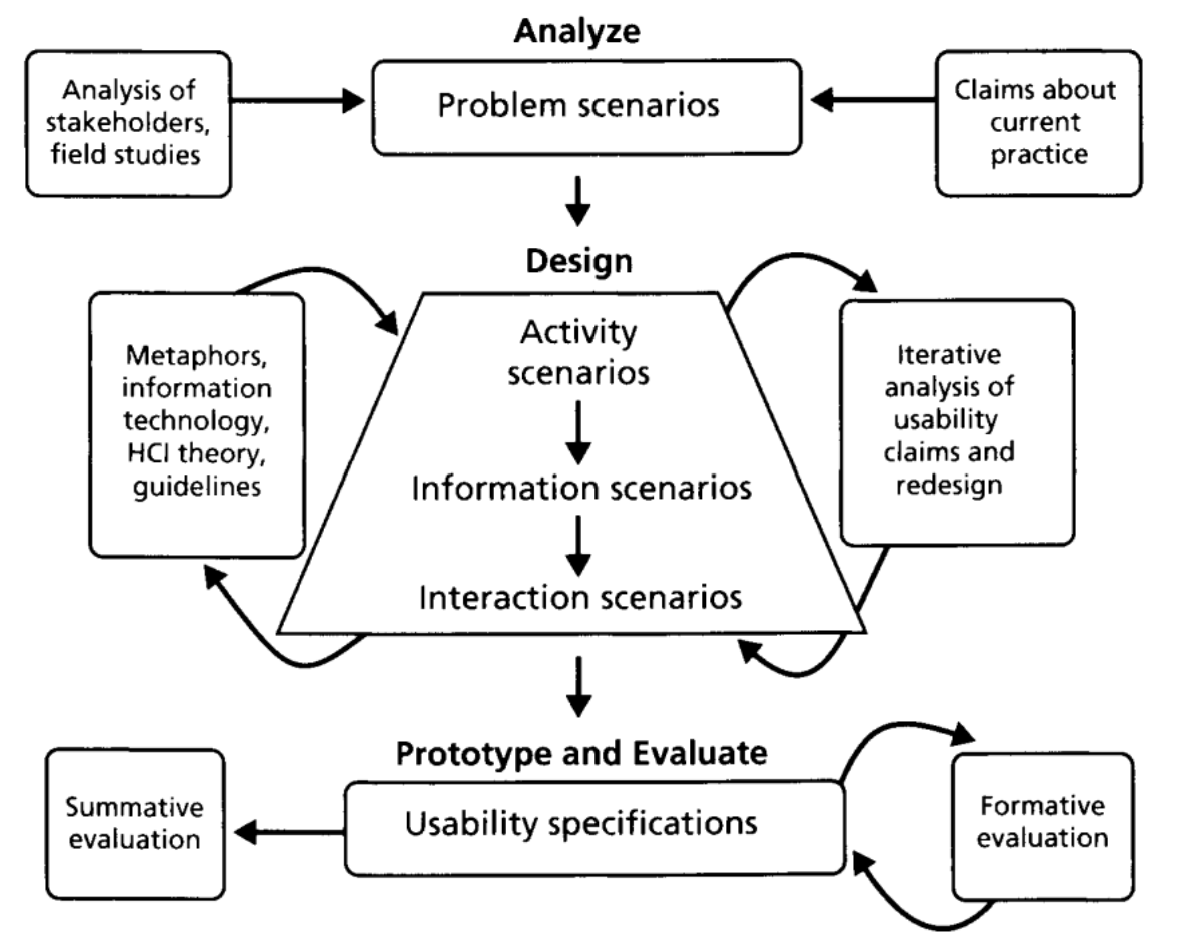
\includegraphics{./tex2pdf.-c803d322dfea80aa/e706dd62fa4a06e8ad5c31ed0d657fd3a87224be.png}
\caption{Szenario Based-Design aus
{[}\protect\hyperlink{ref-sbd}{1}{]}}\label{fig:sbd}
}
\end{figure}

\hypertarget{sec:context}{%
\section{Kontextanalyse}\label{sec:context}}

Die Kontextanalyse hat zum Ziel zu bestimmen in welchem Zusammenhang
StuMaTo verwendet wird. Dabei sollen die Hauptnutzer identifiziert
werden. Zudem soll analysiert werden, wie sie das aktuelle StuMaTo
verwenden und welche Erwartungen, Erfahrungen und Probleme sie bei der
Benutzung gemacht haben.

\hypertarget{auswahl-der-methodik}{%
\subsection{Auswahl der Methodik}\label{auswahl-der-methodik}}

Für die Kontextanalyse kommen zunächst drei Methoden in Frage:
Fragebogen, Interview und Fokusgruppe. Methoden wie Beobachtungen,
Dokumentenanalyse oder Nutzungstagebücher konnten im vorhinein
ausgeschlossen werden, da Dokumente nicht existieren und
Nutzungstagebücher als zu aufwendig eingestuft werden. Gegen
Beobachtungen spricht, dass sich die Probanden durch die
Corona-Situation im Homeoffice und somit ohne nicht in ihrer gewohnten
Umgebung befinden. So wurde sich für diese Arbeit für die Analyse über
Interviews entschieden. Dabei wird zunächst der Studentenbetreuer in der
Firma PPI AG, in der StuMaTo zum Einsatz kommt, befragt. Er wird
gewählt, da dieser die längste Erfahrung mit der Verwaltung der
Studenten und den besten Überblick über andere Nutzer und Stakeholder
hat. Daraus sollen weitere Stakeholder identifiziert werden. Im
Anschluss daran werden drei Studenten und ein Mitarbeiter, der schonmal
Studenten betreut hat befragt. Somit werden die Sichtweisen aller im
vorhinein identifizierten Nutzergruppen eingeholt.\\
Die Methode Interview wurde gewählt, da sie den Vorteil hat, dass man
mit ihnen die kritischen Ereignisse während der Nutzung des
Softwaresystems aufdeckt werden können. So können die individuellen
Fehler und Hindernisse, die die Nutzer bei der Benutzung des Programmes
erfährt am besten aufgedeckt werden. Zudem bieten sie die Möglichkeit,
dass individuell auf den Befragten eingegangen werden kann und somit die
Probleme unmittelbarer und detaillierter aufgedeckt werden können und
auch neue Aspekte aufgedeckt werden können. Der Nachteil der
Subjektivität der Interviews wird aus der Studentensicht, die in dieser
Arbeit im Vordergrund steht, dadurch abgemildert, dass mehrere Studenten
befragt werden. Somit kann bestimmt werden, ob gewisse Probleme nur
Einzelmeinungen sind oder ob diese mehrere Studenten betreffen. Bei den
beiden anderen Nutzergruppen Mitarbeiter und Studentenbetreuer wird
jeweils nur ein Representant befragt. Dabei muss in der Analyse dieser
Interviews beachtet werden, dass diese Ergebnisse durch eine gewisse
Subjektivität der befragten verzehrt sein könnten. Der Nachteil der
Aufwändigkeit von Interviews wird für diese Arbeit in Kauf genommen. Es
wurde sich gegen eine Fokusgruppe entschieden, da sich bei dieser
Methodik die Teilnehmer gegenseitig beeinflussen können. So wird die
Stimme von sehr meinungsstarken Teilnehmern überrepräsentiert, während
die Probleme weniger meinungsstarker Personen nicht aufgedeckt werden.
Hier kann folglich ein verzerrtes Meinungsbild entstehen. Gegen die
Methodik eines Fragebogens spricht, da standartisierte Fragen nicht
immer passend sind. Hierbei werden nicht so viele Aspekte und Probleme
aufdeckt wie bei einem Interview.

\hypertarget{auswahl-der-interviewfragen}{%
\subsection{Auswahl der
Interviewfragen}\label{auswahl-der-interviewfragen}}

Die Interviewfragen wurden an die verschiedenen Nutzergruppen Student,
Mitarbeiter und Betreuer angepasst. Die meisten Fragen bleiben jedoch
für die unterschiedlichen Nutzergruppen gleich. Insgesamt werden 17
Basisfragen gestellt. Dabei sollen zwei Sachverhalte klären. Erstens der
Firmenkontext und der allgemeine Umgang mit dem Dualen Studium und
zweitens die Verwendung von StuMaTo im Unternehmen. Die Fragen im
Bereich Firmenkontext sollen folgendes klären:

\begin{itemize}
\tightlist
\item
  Wer sind die Stakeholder der Studentenverwaltung
\item
  Wie im Unternehmen kommuniziert wird
\item
  Welche Rolle der Student in den Projekten einnimmt
\item
  Welche Aufgaben neben der Betreuung von Studenten übernommen werden
\item
  Wie das Vermitteln der Aufgaben aktuell abläuft
\item
  Welche Aufgaben für Studenten vorgesehen sind und wie die Betreuung
  ablaufen soll
\item
  Aktueller Einsatz von Softwaretools im Prozess der
  Studentenvermittlung
\end{itemize}

Die Fragen Bereich StuMaTo im Unternehmen sollen zeigen:

\begin{itemize}
\tightlist
\item
  Wie StuMaTo aktuell verwendet wird
\item
  Identifizierte Probleme von StuMaTo
\item
  Verbesserungsvorschläge für StuMaTo
\end{itemize}

\hypertarget{ergebnisse-der-kontextanalyse}{%
\subsection{Ergebnisse der
Kontextanalyse}\label{ergebnisse-der-kontextanalyse}}

H := Hans-Dirk M := Moritz S := Sandra T := Tim F := Finja

\hypertarget{stakeholder-der-studentenverwaltung}{%
\subsubsection{Stakeholder der
Studentenverwaltung}\label{stakeholder-der-studentenverwaltung}}

\hypertarget{ablauf-des-dualen-studiums}{%
\subsubsection{Ablauf des Dualen
Studiums}\label{ablauf-des-dualen-studiums}}

Das Duale Studium an der Nordakademie ist in Blöcken organisiert. Dabei
sind die Blöcke der Theoriephase zehn Wochen lang. Neun Wochen davon
sind Präsenzunterricht und in der letzten Woche werden Prüfungen
geschrieben. In der Praxisphase müssen für die Nordakademie noch
Transfersleistungen geschrieben. Dieses sind kurze wissenschaftliche
Arbeiten im Umfang von etwa zehn Seiten, in denen der Student darlegt,
wie er die Theorie aus dem Studium in der Praxis angewendet hat. Für die
Bearbeitung der Transferleistungen wird den Studenten der PPI AG eine
Bearbeitungszeit in der Arbeitszeit von einer Woche eingeräumt. Die
Theoriephasen können auch unterschiedlich ausfallen. So gibt es für die
Studenten die Möglichkeit, ein Semester im Ausland zu verbringen. Ein
anderes Semester mussten die Studenten aufgrund des Coronavirus von
zuhause aus abhalten.

Nach sieben Semestern Studium und 3,5 Jahren Regelstudienzeit ist das
Duale Studium in der Regel beendet, sofern alle Prüfungen absolviert und
bestanden worden sind. Den Abschluss des Studiums stellt dabei die
Bachelorarbeit dar. Für diese sind die Studenten in der PPI AG auch
komplett freigestellt. (M)

\hypertarget{kommunikation-im-unternehmen}{%
\subsubsection{Kommunikation im
Unternehmen}\label{kommunikation-im-unternehmen}}

Das Betriebsklima in der PPI AG wird insgesamt als sehr angenehm
bezeichnet(S, T, M, F). Dabei ist das Verhältnis zu den Kollegen
konstruktiv und es gibt ein gutes Verhältnis zwischen den Kollegen,
welches sich in einigen Fällen über die Arbeit hinaus erstreckt (T). Es
soll wohl auch vereinzelt persönliche Probleme zwischen einzelnen
Kollegen geben, jedoch ist keiner der Befragten persönlich betroffen
(H). Es konnten auch Unterschiede zwischen verschiedenen Standorten und
Abteilungen festgestellt werden, jedoch wird sich insgesamt an einer
einheitlichen Leitkultur orientiert (M). Zu dieser Leitkultur gehört
unter anderem die ``Du''-Philosophie. In der PPI AG duzen sich
ausnahmslos alle Mitarbeiter untereinander. Zudem gibt es die
Open-Door-Politik, die besagt, dass alle Bürotüren immer offen stehen
sollen und somit direkter Kontakt gefördert werden soll. Somit soll vor
allem die Schwelle zwischen den Mitarbeitern und Vorgesetzten
herabgesetzt werden. (H) Obwohl die Hierachie in der PPI AG möglichst
flach gehalten werden soll, gibt es vier Hierachieebenen: Vorstand,
Bereichsleitung, Abteilungs/Teamleitung und die Mitarbeiter. Diese
Hierarchie ist im Tagesgeschäft aber gar nicht so spürbar (H, T).

\hypertarget{rolle-des-studenten-im-projekt}{%
\subsubsection{Rolle des Studenten im
Projekt}\label{rolle-des-studenten-im-projekt}}

Der Student soll in einem Projekt zunächst Aufgben bearbeiten. Diese
Aufgaben erhält der Student von einem Aufgabenbetreuer. Dabei gibt es
für jeden Studenten genau einen Aufgabenbetreuer, der die Verantwortung
für diesen eine Praxisphase lang übernimmt. Zudem hat der Studenten
verschiedene weitere Ansprechpartner in seinem Projekt. Der
Aufgabenbetreuer ist dabei aber der Hauptansprechpartner und übernimmt
die Einarbeitung. Zudem liefert der Aufgabenbetreuer am Ende eines
Praxiseinsatzes Feedback an den Studentenbetreuer (S). Dabei wird die
Kommmuniktion mit dem Aufgabenbetreuer vorwiegend als positiv bezeichnet
(T). Jedoch sind einige Betreuer manchmal schlecht erreichbar (S,T) oder
es fehlt ihnen an Kompetenz (S). Im Verlauf des Studium nimmt die
Relevanz des Aufgabenbetreuers ab, da die Studenten dann
eigenverantwortlicher arbeiten (T). Im Tagesgeschäft wird der Student
als normaler Mitarbeiter betrachtet, jedoch wird ihm mehr Zeit in der
Bearbeitung der Aufgaben eingeräumt. Dabei wird berücksichtigt, dass der
Student die benötigten Fähigkeiten noch erlernen muss (F). Die meisten
Studenten sind mit der Auswahl der Aufgaben zufrieden und bezeichnen
diese als passend zu ihrem Wissensstand (T, M). Vereinzelt werden die
Studenten als kostengünstige Arbeitskräfte gesehen, was sich auf die
Aufgabenqualität auswirkt (T, F). Zudem sind einige Aufgaben auch nicht
ideal geeignet, da sie zu schnell lösbar waren oder zu schwierig waren
(M).

\hypertarget{aufgaben-neben-der-studentenbetreuung}{%
\subsubsection{Aufgaben neben der
Studentenbetreuung}\label{aufgaben-neben-der-studentenbetreuung}}

Softwaretestmanagement, momentan in großem Kundenprojekt. Kundeneinsatz
ist zurzeit Remote. Ich habe einen Studenten Hauptamtlich betreut, 3
aushilfsweise. Testenwicklung/ Automatisierung Durchführung, Aufgaben
verteilen. Eigentlicher Betreuer hatte Urlaub/Krankheit. (F)

Die Studenten kommen in regelmäßigen Abständen aus der Uni. TFL/Urlaub
muss dazwischen genommen werden. Studenten brauchen dazwischen passende
Aufgaben (F)

\hypertarget{vermittlung-der-aufgaben}{%
\subsubsection{Vermittlung der
Aufgaben}\label{vermittlung-der-aufgaben}}

Da das Studium in Blöcken von abwechselnd Theorie- und Praxisphase
organisiert ist (S), werden die Aufgaben Ende der Theoriephase verteilt,
sodass der Student am Anfang der Praxisphase weiß, in welchem Projekt er
arbeitet (?). Dabei werden die Aufgaben zumeist vom Studentenbetreuer
zugeteilt (S). Der Student darf Wünsche für seine nächste Praxisphase
äußern, jedoch können diese nicht immer erfüllt werden (H). Es besteht
die Möglichkeit sich seinen nächsten Praxiseinsatz auch selber zu
vermitteln, dies kommt jedoch eher selten vor (S). Bei der Zuteilung der
Aufgaben müssen verschiedene Faktoren beachtet werden. Die Aufgabe muss
zum Ausblidungsstand des Studenten passen (F) und zudem soll auf die
Breite in der Ausbildung geachtet werden und den Wünschen des Studenten
entsprechen (H). Des Weiteren muss der Standort der Aufgabe passend sein
(H). Die Aufgaben müssen vom Studentenbetreuer meist aktiv gesucht
werden. Nur selten kommen die Projekte auf den Studentenbetreuer zu,
dass sie einen Studenten brauchen. Dies ist jedoch von Abteilung zu
Abteilung unterschiedlich. In einigen Abteilungen ist es bekannter, dass
es Duale Studenten gibt, in anderen ist es weniger bekannt (H). Der
Erstkontakt für die Vermittlung der Aufgabe wird zwischen dem Studenten
und dem Aufgabenbetreuer hergestellt. Danach wird der Student vom
Studentenbetreuer über seine neue Aufgabe in Kenntnis gesetzt. Danach
meldet sich der Student selbstständig beim Aufgabenbetreuer (H). Für die
Vermittlung der Aufgabe wird von den Studenten der direkte Kontakt zum
Studentenbetreuer gewählt (T). Den Studenten ist es bewusst, dass die
Vermittlung auch über StuMaTo möglich ist, jedoch wird es dafür nicht
verwendet (T, M).

\hypertarget{aufgaben-fuxfcr-studenten}{%
\subsubsection{Aufgaben für Studenten}\label{aufgaben-fuxfcr-studenten}}

Die Studenten unterstützen die Teams und Abteilungen zunächst in ihrer
täglichen Arbeit (S,T). Neben der Unterstützung im Tagesgeseschäft
bekommen Studenten Forschungsaufgaben, in denen neue Technologien und
Ansätze evaluiert und getestet werden (T). Die Aufgaben kommen vor allem
aus den Feldern Softwareentwicklung, Softwaretest und Softwarekonzeption
(F). Zudem übernehmen Studenten auch in Studentenprojekten
Führungsaufgaben und werden im Consulting beim Kunden eingesetzt (M). In
der Ausbildung wird versucht eine möglichst große Breite an Aufgaben für
die Studenten sicherzustellen (H). Dabei werden die Wünsche der
Studenten bei der Aufgabewahl möglichst versucht mit einzubeziehen,
jedoch kann nicht jeder Wunsch erfüllt werden (H). Des Weiteren werden
bei der Auswahl der Aufgaben die Kenntnisse der Studenten
berücksichtigt, jedoch werden auch Aufgaben an Studenten verteilt, für
die die notwendigen Fähigkeiten noch nicht vorhanden sind. Diese sollen
während des Praxiseinsatzes entwicklet werden (F).

\hypertarget{einsatz-von-software-in-studentenverwaltung}{%
\subsubsection{Einsatz von Software in
Studentenverwaltung}\label{einsatz-von-software-in-studentenverwaltung}}

Für die Vermittlung der Studentenaufgaben werden vor allem über Mail,
Chatprogramme und Telefon abgewickelt (M,T,F,H). Die Benutzung des
Mailprogrammes stößt vereinzeilt auf Unmut (T). Dabei wird vor allem die
langsame Kommunikation kritisiert (S). Zudem sorgt die Verwendung von
mehreren firmeninternen Chatprogrammen für Verwirrung (S, F). StuMaTo
wird für die Vermittlung von Aufgaben kaum verwendet (T, F, M). Dabei
stiftet es Verwirrung, dass es aktuell zwei Versionen von StuMaTo gibt
(T). Zudem sind die Daten in StuMaTo nicht alle aktuell (M). StuMaTo
wird von den Studenten vor allem dazu genutzt, um ihr Profil zu pflegen,
um den Mitarbeitern zu demonstrieren, was sie für Aufgaben in der Firma
bearbeitet haben und welche Fähigkkeiten sie dabei erlernt haben. Dabei
ist es den Studenten jedoch unklar, ob sich diese Profile überhaupt
Mitarbeiter in der Firma ansehen. Auf Betreuerseitige wird für das
Zuordnen der Studenten zu den Projekten ein Confluence-Space verwendet.
Eine Übersicht, wann die Studenten verfügbar sind, liefert eine
Exceltabelle. Die Abschlussprotokolle werden mit Word erstellt und per
Mail an die Studenten verschickt (H).

\hypertarget{aktuelle-verwendung-stumato}{%
\subsubsection{Aktuelle Verwendung
StuMaTo}\label{aktuelle-verwendung-stumato}}

StuMaTo wird vor allem zum Pflegen des eigenen Profils verwendet. Dies
dient vor allem zur Representation vor anderen Mitarbietern in der Firma
(S). Dabei werden vor allem die Skills, die die Studenten über die
Einsätze hin erlangt haben, in die Profile mit aufgenommen (M). Zudem
werden die Profile anderer Mitstudenten angesehen (S, M). Dabei werden
sich gerne auch die Transferleistungen von höheren Jahrgängen angesehen
(M). Im neuen StuMaTo können einzelne Klausuren nicht mehr als bestanden
angegeben werden (M). Auch durch die Aufgaben werden gelegentlich
angesehen (T,S), jedoch ist die Aufgabensuche häufig nicht erfolgreich,
da zu wenige im System verfügbar sind (T).Einzelne Mitarbeiter nutzen
StuMaTo, um sich einen Überblick über die Studenten zu verschaffen (F).
Jedoch kennen nicht alle Mitarbeiter StuMaTo oder finden die
Informationen darin nicht verlässlich (M). Dabei sind vor allem diese an
aktuellem Semester und Skills der Studenten interessiert (F). Auf der
Studentenbetreuerseite wird StuMaTo als Sammeltopf für Aufgaben
verwendet (H). Zudem wird über StuMaTo nachverfolgt, welcher Student
welche Aufgabe übernommen hat (H). Für die Nachverfolgung des
Studienstandes wird StuMaTo eher weniger verwendet (H). StuMaTo wird von
den Studenten etwa alle 2 Monate einmal benutzt oder einmal pro Semester
(M,S,T). Bei einigen Studenten hat die Nutzung von StuMaTo über die Zeit
abgenommen und sie benutzen es kaum noch (T). Durchschnittlich wird
StuMaTo von einem Studenten dabei 10 bis 15 Minuten lang benutzt (M,T).
Auch von Mitarbeiterseite werden nur maximal alle zwei Monate
Informationen von StuMaTo abgerufen (F). Die Studentenbetreuer verwenden
StuMaTo hingegen häufiger. Am häufigsten wird es zum Quartalswechsel
benutzt, da dann die Planungsphase für die Praxisphasen der Studenten
beginnt. Dabei wird StuMaTo immer mal für eine bis fünf Minuten benutzt,
ist aber über einen längeren Zeitraum geöffnet (H).

\hypertarget{probleme-in-stumato}{%
\subsubsection{Probleme in StuMaTo}\label{probleme-in-stumato}}

Das häufigstgenannte Problem von StuMaTo ist, dass es keine relevanten
Informationen enthält (T,S). Dabei sind vor allem keine Aufgaben für
Studenten in StuMaTo zu finden (S). Zudem soll es kaum Mitarbeiter
geben, die sich die gepflegten Profile von StuMaTo ansehen (T). Die
Mitarbeiter stellen keine Aufgaben in StuMatO ein, da sie kein Budget
für Studenten oder einfach keine passende Aufgaben für sie haben (F).
Die Studentenbetreuer vermissen in StuMaTo eine Übersicht über die
Verfügbarkeit aller Studenten. Zudem ist es in StuMaTo nicht möglich
Zuteilungen in StuMaTo zu machen, die noch nicht final sind (H).

\hypertarget{ideen-fuxfcr-stumato}{%
\subsubsection{Ideen für StuMaTo}\label{ideen-fuxfcr-stumato}}

Für StuMaTo gibt es verschiedene weitere Ideen. Am häufigsten wurde
genannt, dass die sogenannten Mitarbeitermaster-Profile der
PPI-Mitarbeiter aus den StuMaTo-Profilen generiert werden können. Diese
enthalten ähnliche Informationen wie das StuMaTo-Profil und somit ist
eine unnötige Doppelpflege der Daten notwendig (S, M). Zudem wird sich
eine Rubrik mit allgemeinen Informationen für die Studenten gewünscht
(S). Ein Student wünscht sich StuMaTo als zentrales Tool für die
Studenten zu nutzen und andere Tools wie HR und Controllingsysteme
anzubinden, sodass Urlaubstage aus StuMaTo heraus beantragt werden
können und die Arbeitszeiten eingetragen werden können (M). Dafür wäre
auch eine Kalendarfunktion notwendig (M). Des Weiteren gibt es den
Wunsch, dass die Wünsche der Studenten für die nächste Praxisphase über
StuMaTo eingetragen werden können (H). Zudem könnten die
Studentenabschlussprotokolle über StuMaTo bereitgestellt werden(H).

\hypertarget{reflexion-des-methodeneinsatzes}{%
\subsection{Reflexion des
Methodeneinsatzes}\label{reflexion-des-methodeneinsatzes}}

Insgesamt ist der Einsatz von Interviews für die Analyse des
Nutzungskontext positiv zu bewerten. Es sind lebendige Gespräche
entstanden und durch einige Nachfragen konnten viele Informationen über
den Nutzungskontext von StuMaTo gesammelt werden. Zudem konnten einige
Probleme mit StuMaTo identifiziert werden. Negativ bei der Durchführung
der Interviews ist anzumerken, dass eine explizite Nachfrage zu den
Stakeholdern der Studenten im Unternehmen gefehlt hat. Diese Kategorie
musste aus den anderen Fragen hergeleitet werden. Dies hat zwar halbwegs
funktioniert, jedoch wäre die explizite Frage danach schön gewesen.

\newpage

\hypertarget{sec:heur-anal}{%
\section{Heuristische Analyse}\label{sec:heur-anal}}

\hypertarget{methodik}{%
\subsection{Methodik}\label{methodik}}

Diese Arbeit verwendet eine heuristische Analyse als
Expertenreview-Verfahren um formale Abweichungen von Erfahrungswerten
der Usability festzustellen.

Dies wirkt einerseits ergänzend zu den späteren Nutzerverfahren, welche
tatsächliche Probleme unvoreingenommener Nutzer hervorheben sollen und
andererseits dient es dazu, potentielle Problemfelder zu identifizieren,
welche der Direktion ebenjener Nutzerverfahren dienen können.

Dabei wird im Erfahrungsrahmen der Experten Bezug auf die Artefakte und
Erkenntnisse der Kontextanalyse genommen, um aus dem Kontext der
Anwendung ein erstes Verständnis für Eigenarten, aber auch besondere
Anforderungen von StuMaTo zu erlangen.

\hypertarget{ziele}{%
\subsubsection{Ziele}\label{ziele}}

Der Zweck der heuristischen Analyse ist eine Vertiefung des
Verständnisses für problematische Zustände in der Anwendung.

Daraus ergeben sich hier zwei hauptsächliche Ziele:

\begin{enumerate}
\def\labelenumi{\arabic{enumi}.}
\tightlist
\item
  Die Identifikation von eindeutig nutzerunfreundlichen Elementen zur
  Verwendung in der Gestaltungsphase. Diese sollten klar nutzerfeindlich
  und von lokalisierter Natur sein, sodass daraus entspringende
  Gestaltungsvorschläge unbestreitbar sinnvoll sind und keine
  übergreifenden Prozesse verändern.
\item
  Die Identifikation von Problemfeldern, welche einer genaueren
  Untersuchung bedürfen und somit eine Richtlinie für die Direktion von
  Nutzertests oder weiteren Analysen darstellen. Diese können, durch
  eine Rücksprache mit Stakeholdern und durch weitere Untersuchung
  entweder zu Problemelementen nach Punkt 1 überführt werden, oder zu
  überregionalen Änderungen am Design des Systems führen.
\end{enumerate}

Mögliche Zielartefakte sind demnach Auflistungen dieser.

\hypertarget{art-der-untersuchung}{%
\subsubsection{Art der Untersuchung}\label{art-der-untersuchung}}

Die vorliegende Untersuchung konzentriert sich auf eine heuristische
Analyse unter Zuhilfenahme der Heuristiken nach Nielsen und Shneiderman.

Dies deckt sich vor allem mit dem Ziel, formale Kriterien durch
Expertenwissen nachzuprüfen. Es ist hierdurch möglich, mit gering
gehaltenem Zeitaufwand eine Basis für folgende Untersuchungen durch
Nutzerverfahren zu schaffen, sodass diese Nutzerverfahren nicht
ausschließlich auf der Grundlage der Kontextanalyse geplant werden. Die
enge Verbindung mit den Nutzerverfahren erlaubt es, mithilfe dieser
zusätzlich Fehleinschätzungen während der heuristischen Analyse
aufzudecken.

Das Verfahren der heuristischen Evaluation erlaubt des Weiteren eine
Abdeckung von formalen Kriterien mit begrenztem Expertenwissen und das
sowohl in der Form einer summativen, als auch einer formativen Analyse.

Alternative Expertenverfahren wären zum Beispiel das
Walkthrough-Verfahren und das DaTech-Prüfverfahren. Diese wurden jedoch
unter Bevorzugung der heuristischen Evaluation nicht gewählt.

\textbf{Gegen die Verwendung des Walkthrough-Verfahren sprachen die
folgenden Punkte:}

\begin{itemize}
\item
  Zwei der Autoren hatten bereits eine starke Vertrautheit mit dem
  System, welches eine große Stärke dieses Verfahrens, die Ermittlung
  der explorativen Erlernbarkeit, unterminiert hätten.
\item
  Die Verwendung dieses Verfahrens mithilfe von Nutzern wurde nicht in
  Erwägung gezogen, da dies einen deutlichen logistischen Aufwand für
  einen geringen Mehrwert darstellt, da fokussierte Nutzertests in einem
  Usability-Labor bereits vorgesehen waren.
\item
  Dieses Verfahren einen geringen Fokus auf formale Usability-Prinzipien
  legt. Diese Prinzipien können jedoch für bestimmte Problemklassen eine
  präzisere Begründung für Usability-Probleme liefern, als eine
  subjektive Nutzer-Einschätzung. Die Berücksichtigung der
  Einschätzungen von Nutzern ist jedoch bereits durch die Nutzertests
  geplant und eine ausgeglichene Einschätzung von mehreren Seiten ist
  uns wichtig.
\end{itemize}

\textbf{Gegen die Verwendung des DaTech-Prüfverfahrens sprachen die
folgenden Punkte:}

\begin{itemize}
\item
  Unter der Nutzung des DaTech-Prüfverfahrens ist die Unterscheidung
  zwischen einer schadhaften Abweichung und einer vorteilhaften
  alternativen Gestaltung sehr wichtig. Diese erfordert jedoch eine
  Erfahrung der durchführenden Experten, die wir nicht für uns
  beanspruchen können.
\item
  Eine Zertifizierung der Anwendung ist weder Ziel noch besonders
  hilfreich.
\item
  Grundlegende Prinzipien des Handbuchs sind ebenfalls in den
  Heuristiken der heuristischen Evaluation vorhanden.
\item
  Zum Verständnis des komplexen Prüfhandbuches wäre eine deutlich
  längere Einarbeitung notwendig, welche nicht in einer sinnvollen
  Relation zum Nutzen des Einsatzes in dieser Arbeit stünde, zumal der
  Nutzen, den dieses Verfahren gesondert und im Vergleich zu anderen
  Verfahren zusätzlich bringt, unklar ist.
\end{itemize}

Aus demselben Grund, welcher auch gegen die Verwendung eines
nutzerunterstützten Walkthroughs vorgebracht wurde, wurde sich gegen die
Anwendung einer kooperativen heuristischen Evaluation entschieden.

Stattdessen soll eine heuristische Evaluation aller drei Autoren,
unabhängig voneinander, die großen Probleme der klassischen
heuristischen Evaluation --- ihre geringe Reliabilität und Objektivität
-- einschränken und durch den anschließenden Vergleich aus den
Problemlisten eine gemeinsame, gewichtete Problemliste synthetisieren.

\hypertarget{sec:heuristic:plan}{%
\subsubsection{Ablaufplan}\label{sec:heuristic:plan}}

Diese parallele heuristische Analyse befolgt diesen Ablauf:

\begin{enumerate}
\def\labelenumi{\arabic{enumi}.}
\tightlist
\item
  Kriteriensynthese (in Abschnitt~\ref{sec:heuristic:method:criteria}
  genauer beschrieben)
\item
  Unabhängige Prüfung inkl. Notieren der Probleme
\item
  Erstellung einer gemeinsamen Gesamtliste
\item
  Unabhängige Gewichtung der Probleme der Gesamtliste
\item
  Gewichtung und Probleme diskutieren und zusammenfassen
\item
  Klare und lokalisierte Probleme erfassen und gewichten
\item
  Aus breiteren Trends innerhalb der Probleme Problemfelder erfassen
\item
  Daraus problematische Prozesse und Zustände zum weiteren Test durch
  Nutzer identifizieren
\item
  Im Nachgang zu den Nutzertests Nutzerergebnisse mit Expertenbewertung
  vergleichen
\end{enumerate}

Die Vorbedingung dieses Ablaufes ist die vorangegangene Kontextanalyse.

Punkt 1 bis 5 des dargestellten Ablaufes formen eine klassische
heuristische Analyse dar, welche besonders darauf gerichtet ist,
Beeinflussungen zwischen den Evaluatoren zu vermeiden, indem stets erst
am letzten möglichen Zeitpunkt ein Vergleich der Ergebnisse stattfindet.
So werden zur Vereinheitlichung der Analyse und zur Sicherstellung
auswertbarer Ergebnisse zwar dieselben Kriterien verwendet, die
Bewertung der Anwendung anhand dieser erfolgt jedoch parallel. Nach der
Zusammenführung der gefundenen Probleme erfolgt auch die Gewichtung
dieser wieder parallel.

Punkt 6 bist 8 sind an das Format der Zielstellung gerichtet. Diese
ermöglichen eine sinnvolle Verarbeitung innerhalb des vorgestellen
Analyserahmens.

Punkt 9 dient der Rückkopplung an die Bewertung und kann dazu dienen,
die in Punkt 8 erstellten Problemfelder zu bewerten und Fehler in der
Bestimmung von Problemen in Punkt 6 zu erkennen. Letzteres ist besonders
wichtig, um in der späteren Gestaltungsphase nicht fehlgeleitete, sich
negativ auswirkende Änderungen vorzunehmen. Ersteres hingegen ist die
Grundlage für größere Veränderungen in der Gestaltungsphase.

\hypertarget{sec:heuristic:method:criteria}{%
\subsubsection{Bestimmung der
Analysekriterien}\label{sec:heuristic:method:criteria}}

Die Heuristiken, welche zur Bewertung in dieser Phase der Analyse
verwendet werden, werden durch eine Verbindung der Kriterien nach
Nielsen und der Kriterien nach Shneiderman festgelegt. Diese sind
publiziert und anerkannt und haben dadurch eine kanonische Beschreibung.
Die Verbindung beider Kriterienmengen dient dabei der Vergrößerung des
Bewertungsspektrums und der Verringerung der Abhängigkeit zu einer
Person, die diese publiziert hat.

Diese Kriterien werden zunächst von uns definiert, sehr ähnliche
miteinander verbunden und redundante Kriterien werden eliminiert.
Anschließend erfolgt eine Darstellung aller Kriterien in ihrem finalen
Zustand.

Die Synthese der Kriterien erfolgt gemeinschaftlich, um allen eine
Mitsprache zu erteilen und dennoch einen einheitlichen Konsens zu
erreichen. Eine noch größere Unabhängigkeit der Evaluationen durch die
Erstellung eigener Kriterien je Evaluator wurde vermieden, da diese die
subjektiven Ansichten des Evaluators nicht nur in die Bewertung des Ist-
sondern auch die Festlegung des Sollzustandes einbezogen hätte. Dies
könnte entgegen zu den Zielen des parallelen Konzeptes eine Erhöhung der
Subjektivität zur Folge haben und könnte ebenfalls durch
Meinungsverschiedenheiten zwischen den Evaluatoren zu einem späteren
Zeitpunkt die Auswertung erschweren.

Die im Folgenden verwendeten Kriterien aus
{[}\protect\hyperlink{ref-heur:shneiderman}{2}{]} und
{[}\protect\hyperlink{ref-heur:nielsen}{3}{]} sind im Anhang respektive
unter Abschnitt~\ref{sec:heuristiken-shneiderman} und
Abschnitt~\ref{sec:heuristiken-nielsen} beschrieben.

Alle hier verwendeten Kriterien werden jedoch zugunsten des Leseflusses
ins Deutsche übersetzt und teilweise dabei leicht verändert. Des
Weiteren erhalten Sie eine originale Beschreibung nach dem Verständnis
der heuristischen Evaluatoren, welches durch die Konsultation der eben
genannten Beschreibungen gebildet wurde. Diese erneute Beschreibung und
Bezeichnung sollen Missverständnisse zwischen Lesern und Evaluatoren
vermeiden. Sollte bei der Verwendung der existierenden Kriterien ein
abweichendes Verständnis der Kriterien bei Leser und Evaluator
herrschen, würde dies die Aussagekraft der Analyse für den Leser
mindern.

In der Interpretation der Probleme wird jedoch ausschließlich die
hiesige Definition zu Rate gezogen. Geschieht hierbei eine Verwechslung
oder ein Missverständnis von Kriterien nach Nielsen und Shneiderman, ist
der Vergleich zu diesen zwar schwierig, die Schlussfolgerung der
Entscheidungen dieser Analyse leidet aber nicht.

\hypertarget{analysekriterien}{%
\subsubsection{Analysekriterien}\label{analysekriterien}}

Von den Kriterien nach Nielsen werden folgende Kriterien übernommen:

\begin{itemize}
\item
  ``Aesthetic and Minimalist Design'' als ``Relevanz der
  Kommunikation'', da dieses Kriterium sich besonders auf die Vermeidung
  überflüssiger Informationen und weniger auf die eher subjektive
  Beschreibung der Ästhetik bezieht
\item
  ``Help users recognize, diagnose, and recover from errors'' als
  ``Konstruktive Fehlerbehandlung'', da der Fokus darauf liegt, dem
  Nutzer konkret bei der Behandlung eines Fehlers zu unterstützen
\item
  ``Help and Documentation'' nach
  {[}\protect\hyperlink{ref-heur:brauux2fsarodnick}{4}{]} als ``Hilfe
  und Dokumentation''
\item
  ``Match between system and the real world'' als ``Realitätsnahe
  Semantik und Vokabular'', da die Bedeutung des Kriteriums sich
  besonders auf realitätsnahe Metaphorik konzentriert und weniger auf
  den Zustand der Welt und des Systems.
\end{itemize}

Von den Kriterien nach Shneiderman werden folgende Kriterien übernommen:

\begin{itemize}
\tightlist
\item
  ``Design dialogs to yield closure'' als ``Abgeschlossene Aktionen''
\item
  ``Keep users in control'' nach
  {[}\protect\hyperlink{ref-heur:dahm}{5}{]} als ``Benutzerbestimmte
  Eingaben''
\end{itemize}

Darüber hinaus wird eine Reihe von Kriterien von Shneiderman und Nielsen
aufgrund auftretender Redundanz oder thematischer Ähnlichkeit
kombiniert:

\begin{itemize}
\item
  ``Visibility of system status'' und ``Offer informative feedback.''
  berühren ähnliche Themenkomplexe. Ersteres Kriterium beinhaltet dabei
  über das letztere hinaus auch die Sichtbarkeit länger anhaltenden
  Zustandes, während letzteres sich vor allem auf Zustände als Reaktion
  auf Aktionen bezieht. Diese beiden wurden darum als ``Sichtbarer
  Systemstatus und Statusmeldungen'' zusammengefasst.
\item
  ``User control and freedom'' und ``Permit easy reversal of actions''
  als ``Reversibiltät und Abbruchmöglichkeiten'', da ersteres Kriterium
  das letztere in seiner Beschreibung enthält, aber besonders auch die
  Möglichkeit des Abbruchs zu jeder Zeit hervorhebt.
\item
  ``Consistency and standards'' und ``Strive for consistency.'' als
  ``Konsistenz und Standardtreue'', da sie sich sehr ähneln. Im Detail
  fokussiert sich ersteres eher auf die Konsistenz zu anderen
  Anwendungen und letzteres auf die interne Konsistenz, für den Nutzer
  stellt dies jedoch ein nahezu identisches Problem dar.
\item
  ``Error prevention'' und ``Prevent errors.'' sind als identische
  Kriterien in ``Fehlerprävention'' zusammengefasst.
\item
  ``Recognition rather than recall'' und ``Reduce short-term memory
  load.'' sind ebenfalls in ihrer Intention identisch und wurden nach
  {[}\protect\hyperlink{ref-heur:brauux2fsarodnick}{4}{]} als ``Erkennen
  vor Erinnern'' kombiniert
\item
  ``Flexibility and efficiency of use'' und ``Seek universal
  usability.'', da ersteres in letzterem Kriterium enthalten ist. Dies
  ist als ``Universelle Benutzbarkeit und Anpassbarkeit'' bezeichnet.
\end{itemize}

Das Ergebnis dieses Verfahrens ist in \cref{tbl:mergecriteria} und
\cref{tbl:criteria} aufgeführt.

\begin{longtable}[]{@{}lcr@{}}
\caption{Herleitung der Kriterien der Heuristischen Evaluation
\label{tbl:mergecriteria}}\tabularnewline
\toprule
\begin{minipage}[b]{0.30\columnwidth}\raggedright
Nielsen\strut
\end{minipage} & \begin{minipage}[b]{0.31\columnwidth}\centering
Extrahiertes Kriterium\strut
\end{minipage} & \begin{minipage}[b]{0.30\columnwidth}\raggedleft
Shneiderman\strut
\end{minipage}\tabularnewline
\midrule
\endfirsthead
\toprule
\begin{minipage}[b]{0.30\columnwidth}\raggedright
Nielsen\strut
\end{minipage} & \begin{minipage}[b]{0.31\columnwidth}\centering
Extrahiertes Kriterium\strut
\end{minipage} & \begin{minipage}[b]{0.30\columnwidth}\raggedleft
Shneiderman\strut
\end{minipage}\tabularnewline
\midrule
\endhead
\begin{minipage}[t]{0.30\columnwidth}\raggedright
Match between system and the real world\strut
\end{minipage} & \begin{minipage}[t]{0.31\columnwidth}\centering
Realitätsnahe Semantik und Vokabular\strut
\end{minipage} & \begin{minipage}[t]{0.30\columnwidth}\raggedleft
\strut
\end{minipage}\tabularnewline
\begin{minipage}[t]{0.30\columnwidth}\raggedright
Aesthetic and minimalist design\strut
\end{minipage} & \begin{minipage}[t]{0.31\columnwidth}\centering
Relevanz der Kommunikation\strut
\end{minipage} & \begin{minipage}[t]{0.30\columnwidth}\raggedleft
\strut
\end{minipage}\tabularnewline
\begin{minipage}[t]{0.30\columnwidth}\raggedright
Help users recognize, diagnose, and recover from errors\strut
\end{minipage} & \begin{minipage}[t]{0.31\columnwidth}\centering
Konstruktive Fehlerbehandlung\strut
\end{minipage} & \begin{minipage}[t]{0.30\columnwidth}\raggedleft
\strut
\end{minipage}\tabularnewline
\begin{minipage}[t]{0.30\columnwidth}\raggedright
Help and documentation\strut
\end{minipage} & \begin{minipage}[t]{0.31\columnwidth}\centering
Hilfe und Dokumentation\strut
\end{minipage} & \begin{minipage}[t]{0.30\columnwidth}\raggedleft
\strut
\end{minipage}\tabularnewline
\begin{minipage}[t]{0.30\columnwidth}\raggedright
\strut
\end{minipage} & \begin{minipage}[t]{0.31\columnwidth}\centering
\strut
\end{minipage} & \begin{minipage}[t]{0.30\columnwidth}\raggedleft
\strut
\end{minipage}\tabularnewline
\begin{minipage}[t]{0.30\columnwidth}\raggedright
\strut
\end{minipage} & \begin{minipage}[t]{0.31\columnwidth}\centering
Abgeschlossene Aktionen\strut
\end{minipage} & \begin{minipage}[t]{0.30\columnwidth}\raggedleft
Design dialogs to yield closure.\strut
\end{minipage}\tabularnewline
\begin{minipage}[t]{0.30\columnwidth}\raggedright
\strut
\end{minipage} & \begin{minipage}[t]{0.31\columnwidth}\centering
Benutzerbestimmte Eingaben\strut
\end{minipage} & \begin{minipage}[t]{0.30\columnwidth}\raggedleft
Keep users in control.\strut
\end{minipage}\tabularnewline
\begin{minipage}[t]{0.30\columnwidth}\raggedright
\strut
\end{minipage} & \begin{minipage}[t]{0.31\columnwidth}\centering
\strut
\end{minipage} & \begin{minipage}[t]{0.30\columnwidth}\raggedleft
\strut
\end{minipage}\tabularnewline
\begin{minipage}[t]{0.30\columnwidth}\raggedright
User control and freedom\strut
\end{minipage} & \begin{minipage}[t]{0.31\columnwidth}\centering
Reversibilität und Abbruchmöglichkeit\strut
\end{minipage} & \begin{minipage}[t]{0.30\columnwidth}\raggedleft
Permit easy reversal of actions.\strut
\end{minipage}\tabularnewline
\begin{minipage}[t]{0.30\columnwidth}\raggedright
Visibility of system status\strut
\end{minipage} & \begin{minipage}[t]{0.31\columnwidth}\centering
Sichtbarer Systemstatus und Statusmeldungen\strut
\end{minipage} & \begin{minipage}[t]{0.30\columnwidth}\raggedleft
Offer informative feedback.\strut
\end{minipage}\tabularnewline
\begin{minipage}[t]{0.30\columnwidth}\raggedright
Consistency and standards\strut
\end{minipage} & \begin{minipage}[t]{0.31\columnwidth}\centering
Konsistenz und Standardtreue\strut
\end{minipage} & \begin{minipage}[t]{0.30\columnwidth}\raggedleft
Strive for consistency.\strut
\end{minipage}\tabularnewline
\begin{minipage}[t]{0.30\columnwidth}\raggedright
Error prevention\strut
\end{minipage} & \begin{minipage}[t]{0.31\columnwidth}\centering
Fehlerprävention\strut
\end{minipage} & \begin{minipage}[t]{0.30\columnwidth}\raggedleft
Prevent errors.\strut
\end{minipage}\tabularnewline
\begin{minipage}[t]{0.30\columnwidth}\raggedright
Recognition rather than recall\strut
\end{minipage} & \begin{minipage}[t]{0.31\columnwidth}\centering
Erkennen vor Erinnern\strut
\end{minipage} & \begin{minipage}[t]{0.30\columnwidth}\raggedleft
Reduce short-term memory load.\strut
\end{minipage}\tabularnewline
\begin{minipage}[t]{0.30\columnwidth}\raggedright
Flexibility and efficiency of use\strut
\end{minipage} & \begin{minipage}[t]{0.31\columnwidth}\centering
Universelle Benutzbarkeit und Anpassbarkeit\strut
\end{minipage} & \begin{minipage}[t]{0.30\columnwidth}\raggedleft
Seek universal usability.\strut
\end{minipage}\tabularnewline
\bottomrule
\end{longtable}

Da in der Kontextanalyse beanstandet wurde, dass das System schlecht
gepflegt und nicht aktuell ist, wird außerdem das Kriterium der
``Aktualität und Pflege'' gesondert betrachtet. Dies ist ein Problem,
welches die Usability des Systems einschränkt, ohne jedoch zwingend eine
klassische Heuristik zu sein. Der Fakt, dass Inhalte veraltet sind, ist
in sich kein Designfehler, der behoben werden kann, kann sehr wohl
jedoch ein Symptom zugrundeliegender Probleme sein. Darum wurde dieses
Kriterium dennoch geschaffen, um diese Nutzeraussagen nachzuvollziehen
und detaillierter zu verstehen. Hierzu wurden durch \texttt{Hendrik} und
\texttt{Til} Analysen im Produktivsystem vorgenommen, da sie als
Mitarbeiter von \texttt{ppi} auf dieses Zugriff haben.

Aus dem Verständnis dieser Kriterien entsprechend ihrer Beschreibung in
Anhang \ref{sec:heuristik-beschreibungen} werden die folgenden
Beschreibungen synthetisiert:

\begin{longtable}[]{@{}lrl@{}}
\caption{Verwendete Kriterien der Heuristischen Evaluation
\label{tbl:criteria}}\tabularnewline
\toprule
\begin{minipage}[b]{0.09\columnwidth}\raggedright
Bezeichner\strut
\end{minipage} & \begin{minipage}[b]{0.25\columnwidth}\raggedleft
Kriterium\strut
\end{minipage} & \begin{minipage}[b]{0.58\columnwidth}\raggedright
Beschreibung\strut
\end{minipage}\tabularnewline
\midrule
\endfirsthead
\toprule
\begin{minipage}[b]{0.09\columnwidth}\raggedright
Bezeichner\strut
\end{minipage} & \begin{minipage}[b]{0.25\columnwidth}\raggedleft
Kriterium\strut
\end{minipage} & \begin{minipage}[b]{0.58\columnwidth}\raggedright
Beschreibung\strut
\end{minipage}\tabularnewline
\midrule
\endhead
\begin{minipage}[t]{0.09\columnwidth}\raggedright
ADAPT\strut
\end{minipage} & \begin{minipage}[t]{0.25\columnwidth}\raggedleft
Universelle Benutzbarkeit \& Anpassbarkeit\strut
\end{minipage} & \begin{minipage}[t]{0.58\columnwidth}\raggedright
Die Anwendung kann von Anwendern unterschiedlichster mit verschiedenen
Eigenschaften, Fähigkeitsstufen und Erfahrungen verwendet werden. Sowohl
Anfänger, als auch Experten werden vom System adäquat unterstützt, ohne
die jeweils andere Gruppe zu beeinträchtigen. Die Anwendung ist dazu auf
die Bedürfnisse von Nutzern anpassbar.\strut
\end{minipage}\tabularnewline
\begin{minipage}[t]{0.09\columnwidth}\raggedright
CLOSURE\strut
\end{minipage} & \begin{minipage}[t]{0.25\columnwidth}\raggedleft
Abgeschlossene Aktionen\strut
\end{minipage} & \begin{minipage}[t]{0.58\columnwidth}\raggedright
Aktionen sind in sich klar abgeschlossen und es ist offensichtlich, wenn
ein Arbeitsabschnitt beendet ist -- idealerweise bereits vor dem
Abschluss. Ein Nutzer bekommt Feedback bei Abschluss einer
Operation.\strut
\end{minipage}\tabularnewline
\begin{minipage}[t]{0.09\columnwidth}\raggedright
CONSIST\strut
\end{minipage} & \begin{minipage}[t]{0.25\columnwidth}\raggedleft
Konsistenz und Standardtreue\strut
\end{minipage} & \begin{minipage}[t]{0.58\columnwidth}\raggedright
Die Anwendung zeigt für ähnliche Situationen ein gleichartiges Verhalten
und ist demnach wieder erkennbar. Sie hält sich an bekannte Standards in
anderen Systemen, um auch im Bezug zu diesen Wiedererkennbarkeit zu
ermöglichen und erlernbar zu sein.\strut
\end{minipage}\tabularnewline
\begin{minipage}[t]{0.09\columnwidth}\raggedright
CONTROL\strut
\end{minipage} & \begin{minipage}[t]{0.25\columnwidth}\raggedleft
Benutzerbestimmte Eingaben\strut
\end{minipage} & \begin{minipage}[t]{0.58\columnwidth}\raggedright
Die Handlungen im System werden durch den Nutzer bestimmt, er beherrscht
die Interaktion mit dem System. Das System weicht nicht von den
grundlegenden Erwartungen an die Konsequenzen einer Nutzerhandlung hab
und zwingt den Nutzer auch nicht, Handlungen oder Eingaben unnötig zu
wiederholen.\strut
\end{minipage}\tabularnewline
\begin{minipage}[t]{0.09\columnwidth}\raggedright
ERR-HANDLE\strut
\end{minipage} & \begin{minipage}[t]{0.25\columnwidth}\raggedleft
Konstruktive Fehlerbehandlung\strut
\end{minipage} & \begin{minipage}[t]{0.58\columnwidth}\raggedright
Treten Fehler auf, ermöglicht das System dem User mithilfe
verständlicher diagnostischer Hinweise zu reagieren. Diese Hinweise sind
menschenlesbar und bieten wertvolle, konstruktive Hinweise auf
potentielle Fehlerursachen und zu Behebungsmöglichkeiten.\strut
\end{minipage}\tabularnewline
\begin{minipage}[t]{0.09\columnwidth}\raggedright
ERR-PREV\strut
\end{minipage} & \begin{minipage}[t]{0.25\columnwidth}\raggedleft
Fehlerprävention\strut
\end{minipage} & \begin{minipage}[t]{0.58\columnwidth}\raggedright
Der Nutzer wird vom System daran gehindert, destruktive Handlungen --
vor allem unabsichtlich -- auszuführen oder das System in Fehlzustände
zu leiten. Das System ist des Weiteren klar und verständlich, um auch
Verwechslungen und daraus folgende semantische Fehler zu vermeiden.
Unsinnige Eingaben werden nicht zugelassen.\strut
\end{minipage}\tabularnewline
\begin{minipage}[t]{0.09\columnwidth}\raggedright
HELP\strut
\end{minipage} & \begin{minipage}[t]{0.25\columnwidth}\raggedleft
Hilfe und Dokumentation\strut
\end{minipage} & \begin{minipage}[t]{0.58\columnwidth}\raggedright
Es existiert eine Möglichkeit auf Hilfestellungen und
Verhaltensdokumentation des Systems zuzugreifen, falls es nötig
ist.\strut
\end{minipage}\tabularnewline
\begin{minipage}[t]{0.09\columnwidth}\raggedright
REAL\strut
\end{minipage} & \begin{minipage}[t]{0.25\columnwidth}\raggedleft
Realitätsnahe Semantik und Vokabular\strut
\end{minipage} & \begin{minipage}[t]{0.58\columnwidth}\raggedright
Das System verwendet Begriffe und Metaphern aus der realen Welt, mit
denen eine intuitive Verbindung hergestellt werden kann. So erscheint
das System für den Nutzer durch seine Erfahrung mit der Welt logisch und
sinnvoll.\strut
\end{minipage}\tabularnewline
\begin{minipage}[t]{0.09\columnwidth}\raggedright
RECOG\strut
\end{minipage} & \begin{minipage}[t]{0.25\columnwidth}\raggedleft
Erkennen vor Erinnern\strut
\end{minipage} & \begin{minipage}[t]{0.58\columnwidth}\raggedright
Das Kurzzeitgedächtnis des Nutzers wird geschont, indem ein intuitives
Verständnis ermöglicht wird und indem Daten nicht über mehrere Ansichten
hinweg gemerkt werden müssen. Dringend notwendige Informationen können
stets aus der aktuellen Ansicht erlangt werden.\strut
\end{minipage}\tabularnewline
\begin{minipage}[t]{0.09\columnwidth}\raggedright
RELEV\strut
\end{minipage} & \begin{minipage}[t]{0.25\columnwidth}\raggedleft
Relevanz der Kommunikation\strut
\end{minipage} & \begin{minipage}[t]{0.58\columnwidth}\raggedright
Das System beschränkt sich auf die Kommunikation der notwendigen
Informationen. Überschüssige Kommunikation, welche lediglich die
Sichtbarkeit wichtiger Informationen verschlechtert, werden
vermieden.\strut
\end{minipage}\tabularnewline
\begin{minipage}[t]{0.09\columnwidth}\raggedright
STATUS\strut
\end{minipage} & \begin{minipage}[t]{0.25\columnwidth}\raggedleft
Sichtbarer Systemstatus und Statusmeldungen\strut
\end{minipage} & \begin{minipage}[t]{0.58\columnwidth}\raggedright
Relevante interne Zustände des Systems werden dem Nutzer mitgeteilt,
z.B. spezielle Modi in denen er sich befindet, Ladezeiten,
Fehlerzustände, oder der Speicherzustand der aktuell betrachteten Daten.
Besonders wichtig sind hier auch Statusmeldungen als Reaktion auf
Aktionen des Nutzers.\strut
\end{minipage}\tabularnewline
\begin{minipage}[t]{0.09\columnwidth}\raggedright
UNDO\strut
\end{minipage} & \begin{minipage}[t]{0.25\columnwidth}\raggedleft
Reversibilität und Abbruchmöglichkeit\strut
\end{minipage} & \begin{minipage}[t]{0.58\columnwidth}\raggedright
Der Nutzer behält die Kontroller über den Kontrollfluss, er kann
Aktionen abbrechen, sie rückgängig machen und rückgängig gemachte
Aktionen wiederholen. So wird dem Nutzer die Angst vor den Konsequenzen
ungewollter Aktionen genommen.\strut
\end{minipage}\tabularnewline
\begin{minipage}[t]{0.09\columnwidth}\raggedright
UPTODATE\strut
\end{minipage} & \begin{minipage}[t]{0.25\columnwidth}\raggedleft
Aktualität und Pflege\strut
\end{minipage} & \begin{minipage}[t]{0.58\columnwidth}\raggedright
Das System ist gut gepflegt und verwendbar, es existieren notwendige
Datengrundlagen für eine bedeutsame und hilfreiche Interaktion zwischen
Nutzer und System. Das System unterstützt die Interaktion zur
Sicherstellung eines gepflegten Systems.\strut
\end{minipage}\tabularnewline
\bottomrule
\end{longtable}

\hypertarget{weitere-analyse-parameter}{%
\subsubsection{Weitere
Analyse-Parameter}\label{weitere-analyse-parameter}}

Die Funde aus der Bewertung der Anwendung nach den beschriebenen
Heuristiken werden mit ihrem Fundort dokumentiert und gewichtet. Eine
Zuordnung zu mehreren Heuristiken ist möglich, in der nachfolgenden
Auswertung wird ein Problem für Auswertungen bezüglich der Kriterien
dann je einmal unter jeder zugeordneten Heuristik aufgeführt, da ein
Verstoß gegen mehrere Heuristiken damit auch mehrfach gewürdigt werden
sollte. In Auswertungen, die sich nicht spezifisch auf bestimmte
Kriterien beziehen, wird ein Problem jedoch nicht mehrfach gezählt, um
die Gesamtanzahl nicht zu verfälschen. Zur Dokumentation des Fundortes
werden die katalogisierten Ansichten und Dialoge aus Anhang
\ref{sec:appendix:screens} verwendet. Ist ein Problem als Problem der
gesamten Anwendung und nicht eines Dialogs im Besonderen zu verstehen,
so wird kein Fundort zugeordnet.

Die Gewichtung von Problemen, dargestellt in
\cref{tbl:weighting-definition}, ist in 4 Stufen aufgeteilt. Zu beachten
ist hierbei die Bewertungsstufe 0. Diese wurde aufgenommen, da in der
vorgestellten Methodik Evaluatoren auch eine Bewertung der Schwere von
Problemen, die sie nicht angemerkt haben, vornehmen. So kann eine
Uneinigkeit ob der gefundenen Probleme auch in der Auswertung noch
dargestellt und nachvollzogen werden. Die ebenfalls unorthodox
erscheinende Bewertungsstufe 1 signalisiert die Notwendigkeit, die
Gültigkeit eines Problems vermehrt durch Nutzertests abzusichern,
besonders wenn vermutet wird, dass damit nur potentiell bestimmte
Nutzergruppen betroffen sind. Dies bedeutet allerdings nicht, dass
ernsthafte Probleme, die ``nur'' eine gut verstandene, aber vielleicht
kleine Nutzergruppe betreffen, hiermit bewertet werden sollen. So wären
fehlende ``Accessibility''-Features, welche nur eine Gruppe körperlich
eingeschränkter Menschen betreffen, keineswegs pauschal in die
Gewichtung 1 einzuordnen und damit geringer zu bewerten als kosmetische
Probleme. Vielmehr steht die Unklarheit, ob Anforderungen, die eine
gegebene Situation zum Problem machen würden, überhaupt gegeben sind.

\begin{longtable}[]{@{}ll@{}}
\caption{Definition der genutzten Gewichtungskategorien
\label{tbl:weighting-definition}}\tabularnewline
\toprule
Gewichtung & Bedeutung\tabularnewline
\midrule
\endfirsthead
\toprule
Gewichtung & Bedeutung\tabularnewline
\midrule
\endhead
0 & Kein Usability-Problem\tabularnewline
1 & Könnte je nach Nutzer potentiell ein geringes Problem
darstellen\tabularnewline
2 & Kosmetisches Problem mit Einfluss auf das
Nutzungserlebnis\tabularnewline
3 & Problem mit Einfluss auf den Erfolg einer Interaktion\tabularnewline
\bottomrule
\end{longtable}

Da mehrere Evaluatoren im Ablauf der erklärten Methodik eine Gewichtung
abgeben, bevor diese in einer Gewichtung zusammengefasst werden, wird
mit der folgenden Metrik zusätzlich ein Sinn für die Eindeutigkeit der
Gewichtung unter den Evaluatoren geschaffen:

Die Berechnung der Abweichung der Schwere eines Problems ist wie folgt
und drückt damit die Summe der Differenzen zwischen den einzelnen
Bewertungen aus.

\[Sei~g(x),~x\geq1~die~Schwere~nach~Evaluator~Nr.~x. Sei~n~die~Anzahl~der~Evaluatoren.\]
\[Abweichung~\Delta= \sum_{i=1}^{n}{\sum_{j=i+1}^{n}{|g(i)-g(j)|}}\]

Eine höhere Abweichung ist demnach mit einer höheren ``Kontroverse''
zwischen den Bewertern ob der Schwere des Problems zu verstehen. Eine
geringere Abweichung hingegen spricht für einen Konsens.

\clearpage

\hypertarget{ergebnisse}{%
\subsection{Ergebnisse}\label{ergebnisse}}

Der Ablauf nach Abschnitt \ref{sec:heuristic:plan} ist im Anhang
\ref{sec:heuristik-rohergebnisse} gewissentlich dokumentiert. Die
gemeinsame Problemliste ohne Gewichtung, welche zur Durchführung der
Gewichtung verwendet wurde, ist nicht aufgeführt, da diese redundant zur
finalen Ergebnisliste in \cref{tbl:heur:final} ist. Stattdessen werden
die einzelnen Gewichtungen anhand der Problembezeichner in der
\cref{tbl:heur:weighted} aufgeführt.

Aus Gründen der Übersichtlichkeit wird an dieser Stelle jedoch nicht mit
diesen Rohdaten gearbeitet, sondern lediglich mit aggregierten oder
besonders interessanten Teildaten. In der Betrachtung der folgenden
Daten ist zusätzlich zu beachten, dass einige der angemerkten
Usability-Probleme vermutlich auch als reine Implementierungsfehler
gesehen werden können. Sie wurden hier aber in keinster Weise
ausgeschlossen. Das liegt darin begründet, dass eine Unterscheidung von
schlechtem Design und schlechter Implementierung mangels
Aussagekräftiger Systemspezifikation schwierig und potentiell
willkürlich wäre, worunter die Qualität der Ergebnisse und der Methodik
sinken würde. Darüber hinaus schränken diese Probleme, ob
Implementationsfehler oder Designfehler, eine Einschränkung der User
Experience dar und sollten erwähnt werden. Die folgenden Kapitel der
Arbeit sind jedoch nicht auf die Betrachtung solcher Probleme, die als
in dieser Weise uneindeutig erschienen, ausgerichtet. Dies ist möglich,
da eine Betrachtung all der gefunden Usability-Probleme im Detail den
Rahmen dieser Arbeit ohnehin übersteigen würde.

\hypertarget{quantitative-gesamtkennzahlen}{%
\subsubsection{Quantitative
Gesamtkennzahlen}\label{quantitative-gesamtkennzahlen}}

Mit der bloßen Anzahl \(N\) der Problemfunde und deren Gewichtungen
\(G\), sowie der Abweichungen \(\Delta\) kann ein grober Überblick über
die Datenmenge verschafft werden:

Bei der Betrachtung der Rohmenge der Problemfunde ist \(N=72\), wobei
sowohl der Durchschnitt, als auch der Median von \(G\) über alle
Evaluatoren 2 ist. Dies ist nicht weiter verwunderlich, da aufgrund der
festgelegten, diskreten Werte keine besonderen ``Ausreißer'' einen
signifikanten Unterschied zwischen diesen erklären könnten. Diese Werte
sind unter alle Evaluatoren des Weiteren sehr ähnlich, alle erreichten
denselben Median und sehr ähnliche Durchschnitte (zwischen 1,93
\textbar{} 1,96 \textbar{} 2,11). Das arithmetische Mittel über die
finalen Gewichtungen erreich einen leichten Anstieg auf 2,05. Der hier
wirkende Effekt ist vermutlich, dass erst bei der Diskussion der Schwere
der Probleme untereinander ein vollständiges Verständnis für diese
eingetreten ist, wo sie vorher noch unterschätzt wurden.

Zur Betrachtung der der Daten nach Kategorien wurde als zweite
Datengrundlage jeder Datensatz, dem mehrere Kategorien zugeordnet waren,
dupliziert, um diese mehrfachen Datensatz in der Untersuchung der
Kategorien verwenden zu können. Für eine Betrachtung von einzigartigen
Kategorienmengen waren diese Mehrfachzuordnungen zu selten. In der
einzigartigen Kombination einer zugeordneten Kategorie und eines
Problems ergibt sich \(N'=80\).

In Abbildung~\ref{fig:rel-weights} ist die relative Häufigkeit der
einzelnen Gewichtungskategorien ersichtlich.

\begin{figure}
\hypertarget{fig:rel-weights}{%
\centering
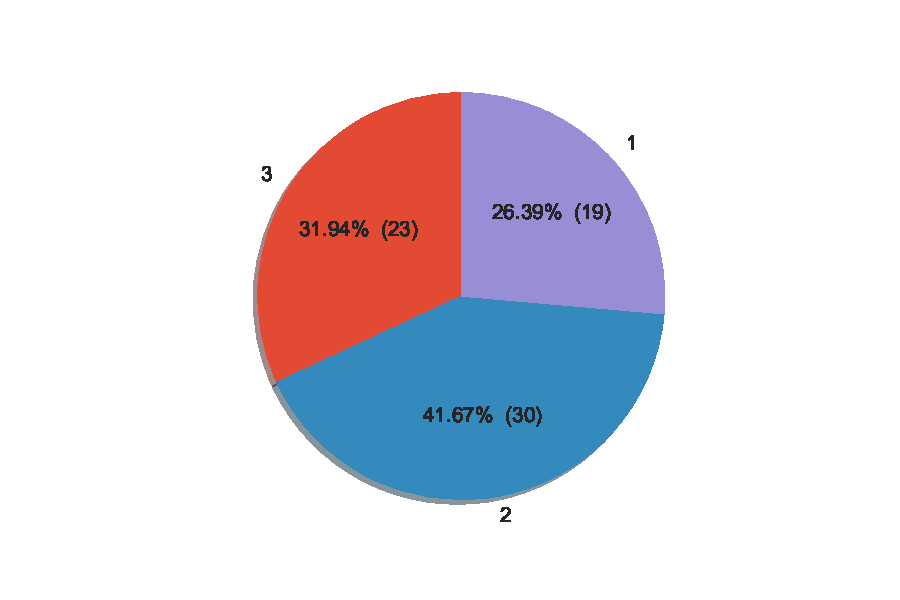
\includegraphics{./tex2pdf.-c803d322dfea80aa/388ffccc4f22fb151ed851faca741ed1f470f666.pdf}
\caption{Relative Gewichtungshäufigkeit}\label{fig:rel-weights}
}
\end{figure}

Die Kategorie \(0\) wurde in der finalen Ergebnisliste effektiv
eliminiert, da diese aussagt, dass hier kein Problem vorliegt. Diese
wurde zwar in den einzelnen Gewichtungen der Evaluatoren insgesamt 8 mal
gewählt, jedoch kam es stets zu einer Einigung, welche die finale
Gewichtung auf einen anderen Wert festgelegt hatte. Dabei wurde häufig
die finale Gewichtung \(1\) gewählt, da die Uneinigkeit darüber, ob ein
Zustand überhaupt ein Problem ist, dafür spricht, dass dieses
entsprechend der Definition der Gewichtung \(1\) nutzergruppenabhängig
sein könnte.

Die anderen Kategorien sind weitesgehend ausgeglichen, auch wenn die
Gewichtung \(2\) am häufigsten auftritt. Dennoch spricht der Anteil von
30\%, welcher auf die Gewichtung \(3\) entfällt dafür, dass die
Anwendung einige ernste Usability-Probleme hat.

\hypertarget{quantitativer-vergleich-der-problemkategorien}{%
\subsubsection{Quantitativer Vergleich der
Problemkategorien}\label{quantitativer-vergleich-der-problemkategorien}}

Ein quantitativer Vergleich der einzelnen Problemkategorien ist in
Abbildung~\ref{fig:weight-per-category} und
Abbildung~\ref{fig:delta-per-category} vorgenommen. Hier können zum
einen die Häufigkeit, mit der Gewichtungen im finalen Ergebnis
aufgetaucht sind, pro Kategorie nachverfolgt werden und gleichzeitig der
Konsens zwischen den Evaluatoren bezüglich einer Kategorie betrachtet
werden.

In der Häufigkeit der Problemgewichtungen sticht die Kategorie CONTROL
mit einem besonders hohen Anteil von schweren Problemen heraus. Eben
diese wird jedoch auch mit einem vergleichsweise hohen
durchschnittlichen Abweichungswert heraus. Scheinbar scheinen hier also
potentiell schwere Probleme aufzutreten, die jedoch nicht besonders klar
verstanden sind. Das Kriterium CONSIST ist ebenfalls ein sehr
umstrittenes Kriterium, welches zudem die größte absolute
Problemhäufigkeit aufweist, wobei diese Probleme jedoch überwiegend
kosmetischer Art oder sogar nutzergruppenabhängig sind. Noch
umstrittener, wenn auch leicht weniger häufig sind die Probleme der
Kategorie RELEV.

Im Gegensatz hierzu fällt das Kriterium ERR-PREV auf: Trotz dessen, dass
es eine hohe Zahl an Problemen aufweist, besteht hier eine weitaus
geringere Abweichung zwischen den Evaluatoren. Es erscheint dadurch
klar, dass die Anwendung einiges Verbesserungspotential in der
Fehlerprävention aufzuweisen hat. Die quantitativ unscheinbar wirkenden
Kategorien CLOSURE, ERR-HANDLE und UNDO sind in völliger Einstimmigkeit
bewertet worden. Hier treten des Weiteren vermehrt Probleme der
Gewichtung \(3\) auf.

\newpage

\begin{figure}[t]
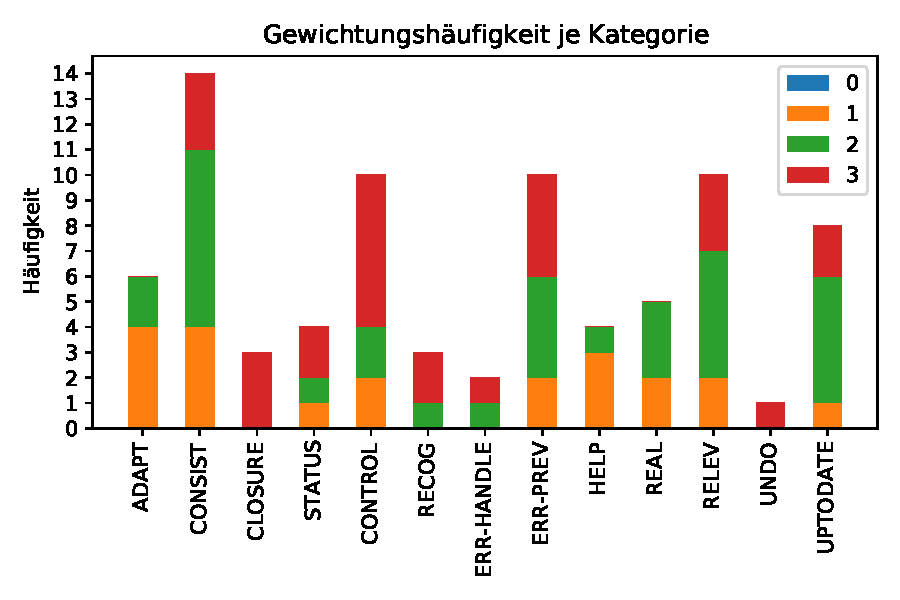
\includegraphics{src/images/stacked-bar.pdf}
\caption{Gewichtungshäufigkeit je Kategorie}
\label{fig:weight-per-category}
\end{figure}
\begin{figure}[b ]
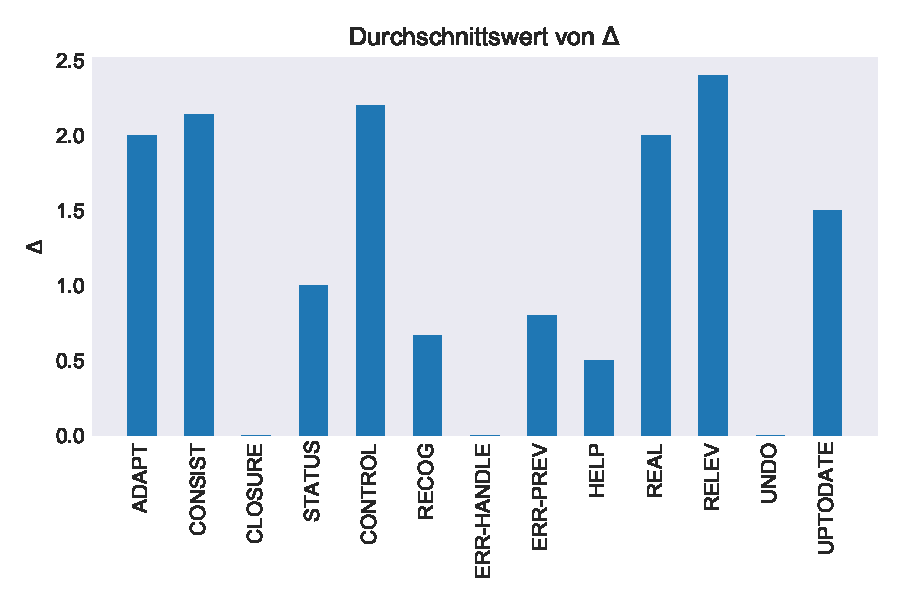
\includegraphics{src/images/bar-dev.pdf}
\caption{Durchschnittsabweichung je Kategorie}
\label{fig:delta-per-category}
\end{figure}

\clearpage

Da besonders ERR-HANDLE und UNDO besonders eng mit ERR-PREV verwandt
sind, scheint generell ein größeres Problempotential in der Peripherie
von Fehlern zu bestehen. Der Umstand, dass die Kategorie UNDO lediglich
ein Problem aufweist, wird hier von der Beschreibung dieses Problems,
welches sich auf die gesamte Anwendung bezieht, überwogen: ``Keine
Möglichkeit, Änderungen rückgängig zu machen oder auch nur
nachzuverfolgen''. Das durch die Kontextanalyse mit aufgenommene
Kriterium UPTODATE hat durchaus eine überdurchschnittliche Menge an
Problemen, meist kosmetischer Natur, mit großer Varianz hervorgerufen.
Es sollte demnach in den Nutzertests weiterverfolgt werden, um mögliche
Gründe für die schlechte Pflege des Systems herauszuarbeiten.

Entsprechend dieser Analyse der Aggregatsdaten erscheint es sinnvoll,
besonders den Umgang mit Fehlern in der Anwendung in den folgenden
Nutzertests zu untersuchen. Eine Möglichkeit zur Nachverfolgung und zur
Wiederherstellung von Systemzuständen sollte in der Designphase
zumindest in Erwägung gezogen werden, besonders wenn Gebiete mit
besonders hohen Fehlerquoten identifiziert werden können. Das
Themengebiet Fehlerbehandlung kann damit ganzheitlich als Problemfeld
entsprechend Ziel Nr. 2 der Heuristischen Evaluation betrachtet werden.
Besonders kritisch sollte auch das Kriterium CONTROL betrachtet werden.
Dieses ist in seiner Definition und in der Sicherheit der Probleme
weniger klar, was eine Nachverfolgung und Verifikation in Nutzertests
jedoch aufgrund der Signifikanz der potentiellen Probleme sehr
interessant macht. Auch dieses Kriterium ist demnach so ein Problemfeld.

Diese Aggregation zeigt jedoch keine Kriterien, welche besonders für ein
Extraktion von klaren, lokalisierten und kosmetischen Problemen nach
Ziel Nr. 1 geeignet wären - zum Einen, da Problemkriterien ohnehin eine
relativ breite Klassifikation wären, welche für konkrete, lokale
Probleme eher weit gefasst wäre, und zum Anderen, da die Kriterien mit
einer großen Menge von kosmetischen Problemen (Gewichtung \(2\)) auch
eine hohe Abweichung zwischen den Evaluatoren aufweisen. Demnach ist es
nicht ohne Weiteres möglich, diese als eindeutig nutzerunfreundlich
herauszustellen.

\hypertarget{betrachtung-von-einstimmig-gewichteten-probleme}{%
\subsubsection{Betrachtung von einstimmig gewichteten
Probleme}\label{betrachtung-von-einstimmig-gewichteten-probleme}}

Aufgrund der Beschränkungen dieser Arbeit, können nicht alle Probleme in
gleicher Art analysiert und für die weitere Betrachtung verwendet
werden. Sehr wohl können jedoch bestimmte Probleme genauer betrachtet
werden. Im vorangehenden Abschnitt wurden bereits einige Kriterien
genannt, welche eine besonders geringe Abweichung zwischen den
Evaluatoren vorwiesen. Hier wird auf diese Aggregation nach Kriterien
verzichtet und es werden als Auszug der Gesamtdaten stattdessen Probleme
betrachtet, welche einstimmig mit der Gewichtung \(3\) oder \(2\)
versehen wurden.

In \cref{tbl:critical-problems} und \cref{tbl:cosmetical-problems} sind
deshalb jene Probleme, welche respektive eine einstimmige Gewichtung von
\(3\) oder \(2\) erhalten haben, aufgelistet.

\begin{longtable}[]{@{}cccc@{}}
\caption{Kritische Probleme (einstimmig)
\label{tbl:critical-problems}}\tabularnewline
\toprule
\begin{minipage}[b]{0.11\columnwidth}\centering
Bezeichner\strut
\end{minipage} & \begin{minipage}[b]{0.13\columnwidth}\centering
Kriterium\strut
\end{minipage} & \begin{minipage}[b]{0.33\columnwidth}\centering
Beschreibung\strut
\end{minipage} & \begin{minipage}[b]{0.32\columnwidth}\centering
Fundorte\strut
\end{minipage}\tabularnewline
\midrule
\endfirsthead
\toprule
\begin{minipage}[b]{0.11\columnwidth}\centering
Bezeichner\strut
\end{minipage} & \begin{minipage}[b]{0.13\columnwidth}\centering
Kriterium\strut
\end{minipage} & \begin{minipage}[b]{0.33\columnwidth}\centering
Beschreibung\strut
\end{minipage} & \begin{minipage}[b]{0.32\columnwidth}\centering
Fundorte\strut
\end{minipage}\tabularnewline
\midrule
\endhead
\begin{minipage}[t]{0.11\columnwidth}\centering
ENDLESS-PROFILE\strut
\end{minipage} & \begin{minipage}[t]{0.13\columnwidth}\centering
CLOSURE\strut
\end{minipage} & \begin{minipage}[t]{0.33\columnwidth}\centering
Bei Bearbeitung des Studentenprofils ist der Abschluss von Aufgaben
nicht klar, es kann ewig ohne klare Abfolge editiert werden.\strut
\end{minipage} & \begin{minipage}[t]{0.32\columnwidth}\centering
STUDENT.UNI, STUDENT.WORK\strut
\end{minipage}\tabularnewline
\begin{minipage}[t]{0.11\columnwidth}\centering
CP-FEEDBACK\strut
\end{minipage} & \begin{minipage}[t]{0.13\columnwidth}\centering
CLOSURE\strut
\end{minipage} & \begin{minipage}[t]{0.33\columnwidth}\centering
Das Speichern von Credit Points gibt wenig Feedback bei der Bestätigung
der Eingabe. Insgesamt ist es schwer ersichtlich, dass man die Eingabe
noch manuell abschließen muss, der Prozess ist nicht atomar.\strut
\end{minipage} & \begin{minipage}[t]{0.32\columnwidth}\centering
STUDENT.UNI\strut
\end{minipage}\tabularnewline
\begin{minipage}[t]{0.11\columnwidth}\centering
SKILLS-SAVED\strut
\end{minipage} & \begin{minipage}[t]{0.13\columnwidth}\centering
CLOSURE, STATUS\strut
\end{minipage} & \begin{minipage}[t]{0.33\columnwidth}\centering
Das Verändern der Kenntnisse ruft keine Speicheroperation hervor und
durch eine Speicheroperation wird keine Rückmeldung hervorgerufen, die
die Aktion für den Nutzer abschließt\strut
\end{minipage} & \begin{minipage}[t]{0.32\columnwidth}\centering
STUDENT.WORK\strut
\end{minipage}\tabularnewline
\begin{minipage}[t]{0.11\columnwidth}\centering
TFL-EDIT\strut
\end{minipage} & \begin{minipage}[t]{0.13\columnwidth}\centering
CONTROL\strut
\end{minipage} & \begin{minipage}[t]{0.33\columnwidth}\centering
Eingetragene TFLs können nicht editiert, sondern nur neu angelegt
werden.\strut
\end{minipage} & \begin{minipage}[t]{0.32\columnwidth}\centering
STUDENT.UNI\strut
\end{minipage}\tabularnewline
\begin{minipage}[t]{0.11\columnwidth}\centering
TASK-FOR-CALENDAR\strut
\end{minipage} & \begin{minipage}[t]{0.13\columnwidth}\centering
CONTROL, RECOG\strut
\end{minipage} & \begin{minipage}[t]{0.33\columnwidth}\centering
Beim Anlegen eines neuen Kalendereintrags sind Aufgaben schwer
auffindbar und können nicht neu angelegt werden. Der Nutzer muss sich
den Namen der Aufgabe gemerkt haben.\strut
\end{minipage} & \begin{minipage}[t]{0.32\columnwidth}\centering
STUDENT.WORK.NEW-ENTRY\strut
\end{minipage}\tabularnewline
\begin{minipage}[t]{0.11\columnwidth}\centering
NO-ERROR-TFL-UPLOAD\strut
\end{minipage} & \begin{minipage}[t]{0.13\columnwidth}\centering
ERR-HANDLE\strut
\end{minipage} & \begin{minipage}[t]{0.33\columnwidth}\centering
Bei einem provozierten Fehler wurde kontinuierlich gespeichert, ein
Abbrechen war nicht möglich oder keine Fehlermeldung wurde angezeigt.
(Hochladen von Dateien)\strut
\end{minipage} & \begin{minipage}[t]{0.32\columnwidth}\centering
STUDENT.UNI.NEW-TFL\strut
\end{minipage}\tabularnewline
\begin{minipage}[t]{0.11\columnwidth}\centering
DIRTY-PROFILE-LEAVE\strut
\end{minipage} & \begin{minipage}[t]{0.13\columnwidth}\centering
ERR-PREV\strut
\end{minipage} & \begin{minipage}[t]{0.33\columnwidth}\centering
Bei editierten Credit Points oder Kenntnissen im Profil keine Nachfrage
beim Verlassen der Seite\strut
\end{minipage} & \begin{minipage}[t]{0.32\columnwidth}\centering
STUDENT.WORK\strut
\end{minipage}\tabularnewline
\begin{minipage}[t]{0.11\columnwidth}\centering
CANCEL-TASK-EDIT\strut
\end{minipage} & \begin{minipage}[t]{0.13\columnwidth}\centering
ERR-PREV\strut
\end{minipage} & \begin{minipage}[t]{0.33\columnwidth}\centering
Kein Nachfragen wenn geänderte Aufgabe nicht gespeichert und dann
abgebrochen oder die Seite verlassen wird\strut
\end{minipage} & \begin{minipage}[t]{0.32\columnwidth}\centering
TASK.EDIT\strut
\end{minipage}\tabularnewline
\begin{minipage}[t]{0.11\columnwidth}\centering
ADD-SKILL-WITH-DIRTY\strut
\end{minipage} & \begin{minipage}[t]{0.13\columnwidth}\centering
ERR-PREV\strut
\end{minipage} & \begin{minipage}[t]{0.33\columnwidth}\centering
Wenn man eine Kenntnis verändert, nicht speichert und dann eine neue
Kenntnis hinzufügt dann werden die Änderungen an der ersten Kenntnis
verworfen.\strut
\end{minipage} & \begin{minipage}[t]{0.32\columnwidth}\centering
STUDENT.WORK\strut
\end{minipage}\tabularnewline
\begin{minipage}[t]{0.11\columnwidth}\centering
UNSEEN-DIRTY\strut
\end{minipage} & \begin{minipage}[t]{0.13\columnwidth}\centering
RECOG, STATUS, ERR-PREV\strut
\end{minipage} & \begin{minipage}[t]{0.33\columnwidth}\centering
Nicht abzusehen ob eine editierte Aufgabe,CP,Kenntnisse bereits
gespeichert oder noch ``dirty'' ist.\strut
\end{minipage} & \begin{minipage}[t]{0.32\columnwidth}\centering
STUDENT.*\strut
\end{minipage}\tabularnewline
\begin{minipage}[t]{0.11\columnwidth}\centering
UNDO\strut
\end{minipage} & \begin{minipage}[t]{0.13\columnwidth}\centering
UNDO\strut
\end{minipage} & \begin{minipage}[t]{0.33\columnwidth}\centering
Keine Möglichkeit, Änderungen rückgängig zu machen oder auch nur
nachzuverfolgen\strut
\end{minipage} & \begin{minipage}[t]{0.32\columnwidth}\centering
*\strut
\end{minipage}\tabularnewline
\begin{minipage}[t]{0.11\columnwidth}\centering
NO-TASKS\strut
\end{minipage} & \begin{minipage}[t]{0.13\columnwidth}\centering
UPTODATE\strut
\end{minipage} & \begin{minipage}[t]{0.33\columnwidth}\centering
Keine Aufgaben sind im Startbereich zu sehen\strut
\end{minipage} & \begin{minipage}[t]{0.32\columnwidth}\centering
TASK.ALL\strut
\end{minipage}\tabularnewline
\begin{minipage}[t]{0.11\columnwidth}\centering
PROFILES\strut
\end{minipage} & \begin{minipage}[t]{0.13\columnwidth}\centering
UPTODATE\strut
\end{minipage} & \begin{minipage}[t]{0.33\columnwidth}\centering
Profile sind wenig gepflegt und nicht aktuell.\strut
\end{minipage} & \begin{minipage}[t]{0.32\columnwidth}\centering
STUDENT.*\strut
\end{minipage}\tabularnewline
\bottomrule
\end{longtable}

Bei diesen kritischen Problemen fällt besonders die Häufigkeit der
Fundorte STUDENT.*, also aller Unterseiten der Seite ``Studenten'',
insbesondere die Tabs der Studentenprofile, auf. Diese scheinen von
kritischen Problemen geplagt zu sein. Die Probleme könnten hierbei
vermehrt auch Veränderungen am Prozess, in dem sie auftreten, erfordern,
oder aber nicht nur lokal relevant sind. So erscheint es wahrscheinlich,
dass die Möglichkeit, Änderungen nachzuverfolgen und Zustände
wiederherzustellen (Problem UNDO) einen aufwändigeren Design-Prozess
erfordern könnte. Auch die Probleme TASK-FOR-CALENDAR, CP-FEEDBACK oder
ENDLESS-PROFILE könnten einen solchen Aufwand erfordern. Andere, wie
UNSEEN-DIRTY, CANCEL-TASK-EDIT, DIRTY-PROFILE-LEAVE,
ADD-SKILL-WITH-DIRTY erfordern mehr Arbeit der Kategorie
Implementierung, als Design.

\begin{longtable}[]{@{}cccc@{}}
\caption{Kosmetische Probleme (einstimmig)
\label{tbl:cosmetical-problems}}\tabularnewline
\toprule
\begin{minipage}[b]{0.11\columnwidth}\centering
Bezeichner\strut
\end{minipage} & \begin{minipage}[b]{0.13\columnwidth}\centering
Kriterium\strut
\end{minipage} & \begin{minipage}[b]{0.33\columnwidth}\centering
Beschreibung\strut
\end{minipage} & \begin{minipage}[b]{0.32\columnwidth}\centering
Fundorte\strut
\end{minipage}\tabularnewline
\midrule
\endfirsthead
\toprule
\begin{minipage}[b]{0.11\columnwidth}\centering
Bezeichner\strut
\end{minipage} & \begin{minipage}[b]{0.13\columnwidth}\centering
Kriterium\strut
\end{minipage} & \begin{minipage}[b]{0.33\columnwidth}\centering
Beschreibung\strut
\end{minipage} & \begin{minipage}[b]{0.32\columnwidth}\centering
Fundorte\strut
\end{minipage}\tabularnewline
\midrule
\endhead
\begin{minipage}[t]{0.11\columnwidth}\centering
DARK\strut
\end{minipage} & \begin{minipage}[t]{0.13\columnwidth}\centering
ADAPT, CONSIST\strut
\end{minipage} & \begin{minipage}[t]{0.33\columnwidth}\centering
Schlechte Kontraste im Darkmode.\strut
\end{minipage} & \begin{minipage}[t]{0.32\columnwidth}\centering
MANAGE, TASK.*, FAQ, STUDENT.WORK, Lade-Indikatoren,Tabs,\strut
\end{minipage}\tabularnewline
\begin{minipage}[t]{0.11\columnwidth}\centering
SEARCH-LAYOUT\strut
\end{minipage} & \begin{minipage}[t]{0.13\columnwidth}\centering
CONSIST\strut
\end{minipage} & \begin{minipage}[t]{0.33\columnwidth}\centering
Layout von Suchergebnissen ist nicht einheitlich.\strut
\end{minipage} & \begin{minipage}[t]{0.32\columnwidth}\centering
SEARCH\strut
\end{minipage}\tabularnewline
\begin{minipage}[t]{0.11\columnwidth}\centering
NEW-SKILL-REENTRY\strut
\end{minipage} & \begin{minipage}[t]{0.13\columnwidth}\centering
CONTROL\strut
\end{minipage} & \begin{minipage}[t]{0.33\columnwidth}\centering
Suchergebnis wird beim erstellen eines neuen Skills nicht
übernommen.\strut
\end{minipage} & \begin{minipage}[t]{0.32\columnwidth}\centering
TASK.EDIT, STUDENT.WORK\strut
\end{minipage}\tabularnewline
\begin{minipage}[t]{0.11\columnwidth}\centering
WHICH-REQUIRED\strut
\end{minipage} & \begin{minipage}[t]{0.13\columnwidth}\centering
ERR-HANDLE\strut
\end{minipage} & \begin{minipage}[t]{0.33\columnwidth}\centering
Wenn benötigte Felder in der Aufgabenerstellung ausgelassen werden, so
zeigt die Fehlermeldung nicht direkt, welche Felder noch gefüllt werden
müssen, sondern nur, dass Eingaben fehlen.\strut
\end{minipage} & \begin{minipage}[t]{0.32\columnwidth}\centering
TASK.EDIT\strut
\end{minipage}\tabularnewline
\begin{minipage}[t]{0.11\columnwidth}\centering
SKILLS-VALIDATION\strut
\end{minipage} & \begin{minipage}[t]{0.13\columnwidth}\centering
ERR-PREV\strut
\end{minipage} & \begin{minipage}[t]{0.33\columnwidth}\centering
Bei der Erstellung neuer Skills wird keine Validierung
vorgenommen.\strut
\end{minipage} & \begin{minipage}[t]{0.32\columnwidth}\centering
MANAGE.SKILLS\strut
\end{minipage}\tabularnewline
\begin{minipage}[t]{0.11\columnwidth}\centering
REQUIRED\strut
\end{minipage} & \begin{minipage}[t]{0.13\columnwidth}\centering
ERR-PREV\strut
\end{minipage} & \begin{minipage}[t]{0.33\columnwidth}\centering
Benötigte Felder in der Aufgabenerstellung werden nicht vorher
gekennzeichnet.\strut
\end{minipage} & \begin{minipage}[t]{0.32\columnwidth}\centering
TASK.EDIT\strut
\end{minipage}\tabularnewline
\begin{minipage}[t]{0.11\columnwidth}\centering
HOVER\strut
\end{minipage} & \begin{minipage}[t]{0.13\columnwidth}\centering
HELP\strut
\end{minipage} & \begin{minipage}[t]{0.33\columnwidth}\centering
Es fehlen des Öfteren Hover-Texte\strut
\end{minipage} & \begin{minipage}[t]{0.32\columnwidth}\centering
*, bspw. TASK.* für Icon-Buttons\strut
\end{minipage}\tabularnewline
\begin{minipage}[t]{0.11\columnwidth}\centering
DASH-REDUNDANT\strut
\end{minipage} & \begin{minipage}[t]{0.13\columnwidth}\centering
RELEV\strut
\end{minipage} & \begin{minipage}[t]{0.33\columnwidth}\centering
Dashboardbuttons führen immer zum selben, wenn man nicht eingeloggt ist.
Die nicht funktionalen Buttons sind nicht notwendig.\strut
\end{minipage} & \begin{minipage}[t]{0.32\columnwidth}\centering
DASH1\strut
\end{minipage}\tabularnewline
\begin{minipage}[t]{0.11\columnwidth}\centering
EMPTY-TIMELINE\strut
\end{minipage} & \begin{minipage}[t]{0.13\columnwidth}\centering
RELEV\strut
\end{minipage} & \begin{minipage}[t]{0.33\columnwidth}\centering
Leere Timeline, leere Kenntnisse etc. werden angezeigt, ohne Mehrwert zu
erbringen.\strut
\end{minipage} & \begin{minipage}[t]{0.32\columnwidth}\centering
STUDENT.UNI\strut
\end{minipage}\tabularnewline
\begin{minipage}[t]{0.11\columnwidth}\centering
EXPIRED-TASKS\strut
\end{minipage} & \begin{minipage}[t]{0.13\columnwidth}\centering
UPTODATE, ERR-PREV\strut
\end{minipage} & \begin{minipage}[t]{0.33\columnwidth}\centering
Zeitlich abgelaufene Aufgaben wurden als verfügbar angezeigt, auch wenn
sie dezent als abgelaufen gekennzeichnet waren.\strut
\end{minipage} & \begin{minipage}[t]{0.32\columnwidth}\centering
TASK.*\strut
\end{minipage}\tabularnewline
\bottomrule
\end{longtable}

All diese Probleme können sehr simpel und ohne die Veränderung von
bestehenden Prozessen bearbeitet werden und stellen eine Liste von
Problemen entsprechend Ziel Nr. 1 dar.

\hypertarget{fazit}{%
\subsubsection{Fazit}\label{fazit}}

Obgleich der Umfang der in der heuristischen Evaluation gefunden
Probleme sehr groß war, konnte hier eine Teilmenge dieser als
unmittelbar interessant für die weitere Betrachtung in der Arbeit
charakterisiert werden.

Für die weitere Untersuchung in den Nutzertests haben sich hier der
Umgang mit Fehlern nach den Heuristiken ERR-PREV, ERR-HANDLE und UNDO
aufgrund ihrer problematischen und wenig umstrittenen Natur
herauskristallisiert. Dabei sollte aufmerksam auch auf Probleme
entsprechend der Heuristiken RELEV und CONTROL geachtet werden, welche
noch problematischer, aber auch umstrittener waren. Auch wurden in
\cref{tbl:critical-problems} besonders kritische Probleme aufgeführt,
welche sich zu großen Teilen in den Studentenprofilen wiederfinden.
Diese Profile sollten deshalb der Kern der Nutzertests sein und der
Design-Bestrebungen sein.

Für eine Implementierung von positiv wirkenden Veränderungen ohne grobe
Änderungen am Design wurde besonders \cref{tbl:cosmetical-problems}
herausgearbeitet.

\hypertarget{reflexion-der-methodik}{%
\subsection{Reflexion der Methodik}\label{reflexion-der-methodik}}

Die anwendete Methodik hat anhand dieser Anwendung zu einer Fülle an
Ergebnissen geführt und war so durchaus erfolgreich und es konnten
entsprechend der definierten Ziele sowohl Problemfelder für eine weitere
Untersuchung in den Nutzertests, als auch eine Menge an eher trivialen
Problemen, welche direkt Designveränderungen oder
Implementierungsänderungen dienen könnten. Ebenfalls hat sich die
geringe Pflege des Produktivsystems bestätigt, die es nun zu untersuchen
gilt.

Ein großes Problem dieser Methodik ist der erhöhte Aufwand, welche durch
die Aggregation des Textmaterials in Probleme, welche keine Redundanz
aufweisen, entsteht. Auch die Diskussion der gesammelten Problemfunde
erhöhte diesen. Eine gemeinsame Bewertung hätten diesen Aufwand
womöglich direkt in der Analyse verringert, doch vermutlich auch eine
weniger Unvoreingenommene und individuelle Bewertung hervorgerufen.
Deshalb wurde die präsentierte Methodik gewählt.

Des Weiteren kam es zu Missverständnissen bezüglich der Bedeutung der
Heuristiken, weshalb diese erneut geklärt und Teile der Analyse
wiederholt werden mussten um eine Vergleichbarkeit zu ermöglichen.
Hierin ist eine Schwäche der heuristischen Analyse, besonders mit
mehreren Evaluatoren, zu sehen. Auch kann trotz der Maßnahmen zur
Reduktion des Einflusses der subjektiven Ansichten der Evaluatoren keine
Garantie für die Objektivität der Problemfunde gegeben werden. Hierbei
ist eine Schwäche und Stärke zugleich, dass zwei der Evaluatoren bereits
breite Vorkenntnisse durch ihre Mitarbeit in der Entwicklung der
Anwendung hatten. Dadurch können sie sich als Experten bereits tiefer in
die Anforderungen der Anwendung hineinversetzen, allerdings besteht auch
das Risiko, dass sie durch ihre enge Involvierung mit dem Projekt
bereits blind gegenüber einem Teil der existierenden Probleme geworden
sind und es ihnen schwieriger fällt, sich in einen neuen Nutzer
hineinzuversetzen. Dies ist jedoch in diesem Verfahren weniger drastisch
als es z.B. in Walkthrough-Verfahren wäre.

Ein weiteres Problem der Methodik ist der verstärkte Einsatz der
Quantifizierung der Problemfunde in der Auswertung. Diese ist sehr
hilfreich im Umgang mit der beachtlichen Problemmenge, aber auch
problematisch, da die genutzten Metriken in ihrer Bestimmung auf
mehreren subjektiven Einschätzungen fußten und des Weiteren in ihrer Art
nicht unbedingt vergleichbar sind, zumal die Fundorte nur begrenzt Teil
der Auswertung und kein Teil der Gewichtung eines Problems waren.
Besonders offensichtlich wurde dies in der Betrachtung des Kriteriums
UNDO, welches lediglich mit einem Problem beschrieben wurde, aber
dennoch ein sehr wichtiges Problem darstellen kann. Hier wurde
dementsprechende auf den qualitativen Unterschied aufmerksam gemacht.

Auch die Definition der Gewichtungen selbst ist schwierig und kann
aufgrund von Uneindeutigkeiten zu Missverständnissen führen. Sie waren
hier auf die Ziele der Analyse zugeschnitten, aber die Unterscheidung
von ``eindeutig nutzerunfreundliche Elemente'' von zu untersuchenden
Problemfeldern ist nicht unproblematisch.

Weiterhin können in diesem begrenzten Rahmen nicht alle Ergebnisse
weiterverarbeitet werden - dies spricht allerdings gleichzeitig für die
Menge an gefundenen Problemen. Für eine detailliertere, tiefere Analyse
des gesamten Problembestandes, wäre jedoch nicht die Wahl einer anderen
Methode, sondern vielmehr die Wahl eines kleineren Teilgebiets der
Anwendung notwendig gewesen. Hier erfolgt stattdessen zur Demonstration
der Methodik eine Einschränkung auf Teilgebiete der Problematik.

\hypertarget{sec:lab}{%
\section{Nutzertests}\label{sec:lab}}

\hypertarget{auswahl-der-methodik-1}{%
\subsection{Auswahl der Methodik}\label{auswahl-der-methodik-1}}

Es soll nach der heuristischen Analyse noch ein Usability-Test
durchgeführt werden. In einem Usabilitytest wird die Interaktion
zwischen realen Nutzern mit dem Programm aufgedeckt. Somit können die
Schwächen des Systems noch detailierter erkannt werden. Da es sich um
reale Nutzer des Programms handelt, zeichnen sich die Usabilitytests
durch eine große Realitätsnähe aus. Für diesen Usablity Test wurde sich
für einen Thinking Aloud Ansatz entschieden. Dabei spricht ein Nutzer
aus, was er gerade tut und denkt. Für diesen Ansatz wurde sich
entschieden, da er weitere Aufschlüsse über den Gefühlszustand und die
Meinung des Nutzers über das Programm hervorruft. Von einer Messung der
Zeit in den Usabilitytests wurde abgesehen, da alle Nutzer in den
Interviews angaben, dass sie ohne Zeitdruck mit StuMaTo arbeiten. Zudem
werden die Messzeiten durch das Thinking Aloud verzerrt, da Nutzer
länger brauchen, wenn sie ihre Gedanken formulieren. Somit ist die Zeit
kein relevanter Faktor für die Analyse. Während der Usabilityanalyse
werden mehrere Aspekte aufgezeichnet. So werden die Augen des Probanden
getrackt, sodass analysiert werden kann, wo er gerade hinsieht. Zudem
kann der FaceReader die Stimmung des Nutzers aufzeichnen. Diese beiden
Informationen sind wichtig, um zu erkennen welche auf der Seite
dargestellten Informationen relevant sind und wie sich das Stimmungsbild
des Nutzers bei der Benutzung des Programmes verhält. Nach dem
Usablility-Test wird noch ein Interview mit dem Probanden geführt.
Hierbei soll die persönliche Meinung des Probanden zur gesamten
Interaktion mit dem Programm herausgefunden werden. Bisher hat der
Proband in dem Thinking Aloud seine Meinung zu einzelnen Aspekten
geteilt, jedoch noch keinen ganzheitlichen Blick gegeben. Zudem soll in
dem Interview geprüft werden, wie die Laborsituation den Probanden
beeinflusst hat. So würden sich einige Personen unter Beobachtung und
wissend, dass es sich nicht um reale Daten handelt andere Aktionen
ausführen, als wenn es sich um die reale Situation handeln würde. Zudem
sollen die Probanden nach ihrem Gesamteindruck und
Verbesserungspotentialen befragt werden. Die Punkte, die dabei genannt
werden, sind besonders relevant, da es die Punkte sind, die den Nutzer
so beschäftigt haben, dass sie im Gedächtnis bleiben. Bei der Auswahl
der Probanden wird darauf geachtet, dass alle möglichen Erfahrungslevel
abgebildet werden können. Insgesamt sollen vier Probanden den
Usabilitytest absolvieren. Ein Proband nutzt StuMaTo schon über sein
ganzes Studium hinweg und hat sogar an der Entwicklung mitgearbeitet. Er
kann als Experte für das Programm eingeschätzt werden. Der zweite
Proband hat etwa ein Jahr Erfahrung mit der Nutzung von StuMaTo und ist
somit als durchschnittlicher Nutzer einzuschätzen. Die letzten beiden
Probanden haben gar keine Erfahrungen mit dem Programm. Hiermit werden
Studenten simuliert, der erst neu in die Firma kommen.

\hypertarget{aufgaben-im-usabilitytest}{%
\subsection{Aufgaben im Usabilitytest}\label{aufgaben-im-usabilitytest}}

Den Probanden werden folgende sechs Aufgaben gestellt:

\begin{enumerate}
\def\labelenumi{\arabic{enumi}.}
\tightlist
\item
  Logge dich ein und sieh dich um!
\item
  Siehe dir dein Profil an und ergänze fehlende Inhalte!
\item
  Du hast Praxisphase vom 5.10 zum 28.11 in Hamburg. Suche dir für
  diesen Zeitraum eine Aufgabe!
\item
  Du hast diese Aufgabe nun abgeschlossen, trage sie in dein Profil ein!
\item
  In dieser Praxisphase hast du eine Transferleistung geschreiben. Diese
  hast du mittlerweile bestanden. Trage dies in dein Profil ein!
\item
  In der nächsten Praxisphase möchtest du ein Marketingprojekt für
  StuMaTo machen, finde über StuMaTo einen Mitstudenten mit dem du
  dieses Projekt durchführen kannst!
\end{enumerate}

\hypertarget{auswahl-der-fragen}{%
\subsubsection{Auswahl der Fragen}\label{auswahl-der-fragen}}

Bei der großen Fülle an heuristischen Problemen, die gefunden wurden,
müssen die Aufgaben eingegrenzt werden, da nicht auf alle heuristischen
Probleme eingegangen werden kann. Die erste Einschränkung ist, dass nur
Funktionalitäten im Usabilitytest aufgenommen werden sollen, die
Studenten betreffen. Somit fallen alle Funktionalitäten, die nur für
Betreuer zugänglich sind, wie Studenten-, Kenntnis- und
Hochschulverwaltung raus. Der Schwerpunkt soll dann auf den Abläufen
liegen, die von den Studenten verwendet werden und diese bei denen sie
Probleme identifiziert haben. Die Daten werden dabei aus den Interviews
gezogen. Dort nannten die Studenten bei der aktuellen Nutzung das
Pflegen des eigenen Profils und das Ansehen von anderen Profilen. Das
Pflegen des Profils wird in Aufgabe 2 behandelt, sowie in Aufgabe 4 und
5. Das Ansehen anderer Profile kann in Aufgabe 1 geschehen und in
Aufgabe 6. Auch das Finden von Aufgaben wurde als Use-Case von StuMaTo
genannt, jedoch wird es nicht sehr häufig genutzt. Um zu analysieren,
welche Probleme es dabei entstehen, gibt es Aufgabe drei. Dabei wurde
der Datenbestand der Aufgaben bewusst sehr klein gehalten, sowie es in
den Interviews auch gennant worden ist. Zudem wurde in den Interviews
genannt, dass StuMaTo eher selten, etwa alle zwei Monate einmal, benutzt
wird. In Aufgabe 1 soll dabei herausgefunden, welche Informationen sich
ein Nutzer rein intuitiv ohne feste Aufgabe ansieht. Insgesamt wurde bei
den Aufgaben darauf geachtet, dass möglichst viele Dialoge durchlaufen
werden, um so in allen Dialogen Fehler aufzudecken.

Im folgenden sollen die möglichen Lösungen und Erwartungen an diese
Aufgaben formuliert werden.

\hypertarget{einloggen-und-umsehen}{%
\subsubsection{Einloggen und Umsehen}\label{einloggen-und-umsehen}}

Für den Login werden dem Probanden jeweils Benutzername und Password
vorgegeben. Nachdem der Login erfolgreich ist, werden der Proband mit
einem Registrierungsdialog konfrontiert. In diesem müssen sie ihre
Hochschule, ihren Studiengang, aktuelles Semester, Eintrittsjahr und
ihren Studentenbetreuer angeben. Wenn dies abgeschlossen wird der
Proband auf sein noch leeres Profil weitergeleitet.

Der Proband kann sich im Folgenden sein eigenes leeres Profil ansehen,
sich die Übersicht aller Studenten und Alumni ansehen und sich in deren
Profile genauer ansehen. Dabei kann er auf Informationen stoßen, welche
Praxiseinsätze diese in der Vergangenheit in der Firma absolviert haben
und welche Skills sie haben. Zudem können allgemeine Informationen der
Mitstudenten wie aktuelles Semester, Studiengang und Hochschule
herausgefunden werden. Darüber hinaus können Transferleistungen der
Mitstudenten gefunden werden und deren Studienfortschritt angeguckt
werden.

Der Proband kann sich zudem die Aufgaben ansehen. Dazu muss er in die
Aufgabenübersicht wechseln. In der Aufgabenübersicht gibt es vier
Reiter: ``Einzelaufgaben'', ``Daueraufgaben'', ``Meine Aufgaben'' und
``Alle Aufgaben''. Hier kann sich der Proband alle Reiter durchsehen.
Dabei kann er sich die Aufgaben näher ansehen und Informationen über die
genaue Beschreibung, den Anssprechpartner, Zeitraum und Ort der Aufgabe
ansehen.

Ein weiteres Element mit dem der Nutzer interagieren kann ist die
globale Suche. Hier kann nach Studenten, Aufgaben und Wissenschaftlichen
Arbeiten gesucht und entsprechend gefiltert werden.

\hypertarget{profil-ansehen-und-erguxe4nzen}{%
\subsubsection{Profil ansehen und
ergänzen}\label{profil-ansehen-und-erguxe4nzen}}

Das Profil des Probanden ist auf drei Wege zu erreichen, durch Klick auf
den Reiter mein Profil oder durch Klick auf sein eigenes Profil in der
Studentenübersicht. Der dritte Weg ist sich selbst im Suchfeld zu suchen
und somit auf das Profil zu gelangen. In der Theorie gibt es noch einen
vierten Weg, wenn sich der Proband in der vorherigen Aufgabe nicht
umgesehen hat, ist dieser nach der Registrierung standardmäßig in seinem
Profil.

Das Studentenprofil ist in zwei Teile aufgeteilt: Uni und Praxis. Im
Abschnitt Uni kann der Proband die Angaben zu seinem Studium ändern.
Dies sollte nicht notwendig sein, da er diese Angaben bereits in seinem
Registrierungsdialog gemacht hat. Zudem kann der Proband seine aktuell
erlangten Credit Points angeben. Die Credit Points sind in drei
Kategorien eingeteilt: Klausuren, Hausarbeiten und Seminare. Des
Weiteren kann der Proband eine Wissenschaftliche Arbeit hochladen, wenn
er bereits eine geschrieben hat.

Im Abschnitt Praxis kann der Student seine Skills angeben. Dabei kann er
Skills aus der Skilldatenbank übernehmen oder einen eigenen Skill
erstellen. Bei den Skills kann er sich auf einen von sechs Skillstufen
festlegen. Die Skillstufen sind Neuling, Anfänger, Medium,
Fortgeschritten, Profi und Meister. In der Verfügbarkeitsübersicht
können sich die vergangenen Praxiseinsätze, Theoriephasen und Urlaube
eingesehen werden. Bei den Einsätzen können vergangene und künftige
Praxiseinsätze eingetragen und mit einer Kurzbeschreibung versehen
werden. Einsätze die dort eingetragen werden, werden automatisch in der
Verfügbarkeitsübersicht übernommen.

\hypertarget{aufgabe-fuxfcr-praxisphase-finden}{%
\subsubsection{Aufgabe für Praxisphase
finden}\label{aufgabe-fuxfcr-praxisphase-finden}}

Aufgaben für die nächste Praxisphase findet der Proband in der
Aufgabenübersicht. In der Aufgabenübersicht sind insgesamt sechs
Aufgaben verteilt, zwei davon in der Kategorie Daueraufgaben und vier in
der Kategorie Einzelaufgaben. Unter diesen sechs Aufgaben sind zwei
invalide, eine findet nicht in dem Zeitraum statt, der für diese Aufgabe
genannt worden ist und die andere ist an einem falschen Standort. Der
Proband soll sich nun durch diese Aufgaben durchklicken, sich einlesen
und dann eine Aufgabe wählen, die er interessant findet oder die zu
seinen Skills passt.

Wenn der Proband sich für eine Aufgabe entschieden hat kann er mit einem
Klick auf den Button ``Interesse'' sich für diese Aufgabe bewerben. Im
Hintergrund wird dann eine Mail an den Aufgabenbetreuer gesendet. Eine
andere Möglichkeit wäre es sich außerhalb von StuMaTo bei dem
Aufgabenbetreuer zu melden und sich für diese Aufgabe zu bewerben. Dies
müsste der Proband dann mündlich dem Versuchsbetreuer mitteilen.

\hypertarget{abgeschlossene-aufgabe-in-profil-eintragen}{%
\subsubsection{Abgeschlossene Aufgabe in Profil
eintragen}\label{abgeschlossene-aufgabe-in-profil-eintragen}}

Bei dieser Aufgabe muss der Proband in sein eigenes Profil zurückkehren.
Hier kann er in der Kategorie Einsätze die Aufgabe eintragen. Hier
müssen der Titel, Beginn und Ende der Aufgabe eingetragen werden.
Optional kann eine Kurzbeschreibung zur Aufgabe hinzugefügt werden. Der
eingetragene Titel muss dabei der Originaltitel der Aufgabe sein.

\hypertarget{transferleistung-in-profil-eintragen}{%
\subsubsection{Transferleistung in Profil
eintragen}\label{transferleistung-in-profil-eintragen}}

Bei dieser Aufgabe muss der Proband drei Unteraufgaben erledigen.

Erstens muss die Transferleistung im Profil unter Wissenschaftliche
Arbeiten hinzufügen. Dabei muss er eine Datei hochladen, die dem
Probanden im Downloads-Ordner des Rechners zur Verfügung gestellt wird.
Bei dem Upload muss eine Kategorie angegeben werden. Hier muss der
Proband die Kategorie Transferleistung/Praxisbericht wählen. Zudem
müssen ein Erstellungsdatum und ein Titel der Transferleistung
eingegeben werden. Optional kann auch eine Kurzbeschreibung des Themas
hinzugefügt werden. Zweitens muss die Credit Point Ansicht aktualisiert
werden. Eine bestandene Transferleistung gibt fünf CreditPoints. Diese
müssen zu der Ansicht hinzugefügt werden.

Drittens muss die Zeit eingetragen werden, in der die Transferleistung
bearbeitet worden ist. Dazu muss zunächst eine neue Aufgabe erstellt
werden, die den Status abgeschlossen hat. Dies ist notwendig, da sich
sonst andere auf diese Aufgabe bewerben könnten, was nicht gewünscht
ist. Die Aufgabe für die Transferleistung kann in der Aufgabenübersicht
erstellt werden. Danach kann die Aufgabe in im Profil unter der
Kategorie Einsätze analog zur vorherigen Aufgabe hinzugefügt werden. Ein
entsprechender Hinweis zu diesem Workflow befindet sich im FAQ.

\hypertarget{mitstudenten-fuxfcr-neues-projekt-finden}{%
\subsubsection{Mitstudenten für neues Projekt
finden}\label{mitstudenten-fuxfcr-neues-projekt-finden}}

Beim Finden eines Studenten gibt es zwei Varianten vorzugehen.

Variante eins ist es sich einen Mitstudenten auszusuchen und mit diesem
außerhalb der Anwendung Kontakt aufzunehmen. Der Studenten können dabei
in der Studentenübersicht oder über die Suche gefunden werden.
Interessant bei der Auswahl der Studenten ist es, dass diese in dem
Zeitraum der Aufgabe verfügbar sind und das diese über die geforderten
Fähigkeiten verfügen. Nach Skills kann auch in der Suchfunktion gesucht
werden. Variante zwei ist es eine neue Aufgabe in StuMaTo zu erstellen
und zu warten bis sich ein Mitstudent darauf bewirbt. Bei der Erstellung
der Aufgabe muss sich zunächst zwischen Daueraufgabe und Einzelaufgabe
entschieden werden. Hierbei handelt es sich um eine Einzelaufgabe, da
diese einen einmaligen Charakter und einen festen zeitlichen Rahmen, den
Rest der Praxispahse, hat. Bei der Erstellung der Aufgabe muss sich der
Proband als Ansprechpartner auswählen. Zudem müssen Titel und
Beschreibung hinzugefügt werden. Des Weiteren muss ein zeitlicher Rahmen
für die Aufgabe festgelegt werden. Dabei müssen ein Start- und Enddatum
angegeben werden und eine Aufwandsschätzung in Personentagen angegeben
werden. Auch ein Standort muss für die Aufgabe hinzugefügt werden.
Dieser ist in diesem Fall Hamburg. Bei den eingesetzten Skills ist es
zudem sinnvoll, dass hier ein Skill Marketing hinzugefügt wird. Dieser
ist noch nicht in der Datenbank, somit muss dieser noch zur Datenbank
hinzugefügt werden. Bei der Möglichen Vorangegangenen Aufgaben kann die
Aufgabe StuMaTo-Entwicklung angegeben werden. Wenn die Aufgabe erstellt
ist, ist auch die letzte Aufgabe für den Probanden und somit der
Usabilitytest beendet.

\hypertarget{ergebnisse-des-usabilitytest}{%
\subsection{Ergebnisse des
Usabilitytest}\label{ergebnisse-des-usabilitytest}}

Im Folgenden werden die Erkenntnisse aus dem Usabilitytest näher
erläutert. Es haben sich zwei Kategorien von Resultaten ergeben. Zuerst
werden Probleme, die bei der Nutzung von einzelnen UI Komponenten
aufgetreten sind, genauer beleuchtet. Diese wurden nach Aufgabenstellung
gruppiert. Anschließend werden übergreifende Probleme betrachtet, die in
verschiedenen Masken aufgetreten sind wo Komponenten wiederverwendet
wurden. Dann wird ein Fokus auf die Workflows innerhalb der Anwendung
gelegt mit denen die Probanden besondere Schwierigkeiten hatten. Die
Probanden werden in den folgenden Unterabschnitten mit Proband 1 bis
Proband 4 (abgekürzt mit P1 - P4) identifiziert.

\hypertarget{probleme-mit-ui-komponenten}{%
\subsubsection{Probleme mit UI
Komponenten}\label{probleme-mit-ui-komponenten}}

\textbf{Einloggen:} Bei der Anmeldung sind keinerlei Schwierigkeiten
aufgetreten.

\textbf{Wizard:} Nach der Anmeldung wurde ein Wizard angezeigt um das
Studentenprofil zu initialisieren. Hier sind mehrere Probleme
aufgetreten. P1 versuchte den Studiengang einzutragen, bevor eine
Hochschule ausgewählt wurde. Dies ist aktuell nicht möglich, da
Studiengänge logisch mit einer Hochschule verknüpft sind. Des Weiteren
gab es Schwierigkeiten bei der Benutzung des Zahlen-Feld für das
Semester. Hier haben P1 und P2 versucht in das Feld zu klicken und die
vorhandene Zahl zu ersetzen, was nicht möglich ist. Diese Problematik
tritt in späteren Aufgaben wieder auf. Proband 4 hat versucht den
Betreuer als Freitext einzugeben. Das Feld ist jedoch ein nicht
optionales Suchfeld bei dem ein Wert aus den Ergebnissen ausgewählt
werden muss. Dies führte zu einer unverständlichen Fehlermeldung. Im
weiteren Verlauf hat dies Schwierigkeiten verursacht\footnote{Da das
  Profil nicht initialisiert war und der Proband über die Navigation den
  Wizard verlassen hat, befand sich die Anwendung in einem
  inkonsistenten Zustand} und der Versuchsbetreuer musste eingreifen.

\textbf{Umschauen:} Diese Aufgabe hat nur geringe Probleme verursacht.
P1 und P2 haben relevante Texte (Dashboard \& FAQ) nur überflogen obwohl
diese im späteren Verlauf relevant waren. Die Verfügbarkeitsdarstellung
im Profil hat bei P1 für zusätzliche Verwirrung gesorgt, da unklar war
was dieser darstellt und wie man damit interagieren kann. Außerdem ist
P3 darauf gestoßen, dass der Zurück-Knopf in einer Daueraufgabe nicht zu
dem Tab der Daueraufgaben zurück führt\footnote{Tatsächlich ist es nur
  eine Weiterleitung zur Einzelaufgaben-Liste, was in späteren Aufgaben
  weitere Probleme verursacht}.

\textbf{Profil pflegen:} Die Verfügbarkeitsdarstellung, welche P1 in der
vorigen Aufgabe bereits entdeckt hat wurde hier von den restlichen
Probanden mit einer ähnlichen Reaktion bemerkt. Bei den Credit-Points
gab es Schwierigkeiten mit der Eingabe von Zahlen wie bereits aus dem
Wizard bekannt. P4 hat den Speichern-Knopf bei den Credit-Points
übersehen und die Seite ohne zu speichern verlassen. Außerdem sprachen
P1 und P2 Verwirrung über die Kategorie ``Hausarbeiten'' aus und waren
sich unsicher was darunter fällt. Bei den Studiums-Einstellungen hat P4
versucht den modalen Dialog per Klick außerhalb des Overlays zu
schließen, was nicht möglich ist. P2 war bei den wissenschaftlichen
Arbeiten unklar was mit Erstellungsdatum gemeint ist, da die meisten
Arbeiten über einen Zeitraum erstellt und anschließend bewertet werden.
Bei den Kenntnissen gab es mehrere Schwierigkeiten. P1 hat einen Begriff
eingetippt und Enter gedrückt bevor die Suchergebnisse geladen haben.
Dies führt dazu, dass das Textfeld geleert aber keine Kenntnis
eingetragen wurde. Probanden 1 bis 3 haben außerdem kritisiert, dass es
keinen Status-Indikator beim Laden von Suchergebnissen oder hinzufügen
von Ergebnissen gibt. Alle vier Probanden haben vergessen die Kenntnisse
zu speichern nachdem sie hinzugefügt wurden\footnote{Hier ist zusätzlich
  eine Inkonsistenz aufgefallen: Wird eine Kenntnis hinzugefügt so
  speichert die Anwendung dies. Dabei werden allerdings sämtliche zuvor
  getätigten ungesicherten Änderungen verworfen. Ändert man den
  Kenntnisstand so muss hingegen explizit gespeichert werden.} und das
obwohl P1 die Speichern-Schaltfläche mehrfach angeschaut hat. Außerdem
haben Probanden 1 und 2 angemerkt, dass es sie verwirrt das die
Kenntnisstände nicht von 0\% bis 100\% sondern von 10\% bis 90\% gehen.
Proband 2 hat versucht eine neue Kenntnis zu erstellen. Dabei war das
Format der notwendigen URL unklar, die Fehlermeldung hat jedoch
ausreichend Hilfestellung gegeben. Kommen wir nun zu den Einsätzen. Hier
wurde das Textfeld für die Aufgabe von den Probanden 1, 2 und 4 als
Freitext wahrgenommen. Nachdem die Fehlermeldung auf diesen Trugschluss
hingewiesen hat wurde von den drei Probanden angemerkt, dass ihnen die
Datenquelle für die Suche unklar ist. Proband 2 hat durch das visuelle
Feedback von dem Eingabefeld erwartet, dass mehrere Aufgaben ausgewählt
werden können. Weitere Schwierigkeiten hatten die Probanden mit den
Eingabefeldern für den Zeitraum des Einsatz. P2 und P4 war unklar, dass
der Zeitraum aus der Aufgabe automatisch übernommen wird. Da diese
Probanden das Datum vor der Aufgabe eingetragen haben wurden ihre Daten
überschrieben. Außerdem sind Probleme mit der Validierung dieser Felder
aufgetreten. Die Felder waren durch die Aufgabe auf ein Datum in der
Vergangenheit initialisiert worden. Probanden 2 und 4 haben daraufhin
das Startdatum angepasst, welches dann nach dem Enddatum lag. Die
Anwendung hat daraufhin eine Fehlermeldung ausgegeben und den Wert
zurückgesetzt. Dieses Zurücksetzen wurde von beiden Probanden nicht
bemerkt.

\textbf{Aufgabe aussuchen:} Probanden 1 und 3 haben als Lösungsansatz
die Suche verwendet und als Suchbegriff den Standort genutzt. Dabei hat
Proband 1 angemerkt, dass die Zugehörigkeit von den Checkboxen zu den
Labels bei den Filtern unklar war. Außerdem wurde angemerkt, dass der
Status (P1) und das Datum der Aufgabe (P3) nicht in den Suchergebnissen
sichtbar ist. Nachdem über die Ergebnisse zu einer Aufgabe navigiert
wurde war unklar, wie man zurückkehren kann. Proband 1 hat versucht die
Suche erneut durchzuführen, hatte allerdings aufgrund eines fehlenden
Buttons im Suchfeld Schwierigkeiten. Proband 3 hat die
Zurück-Schaltfläche in der Aufgabe benutzt, welche wie bereits zuvor
erwähnt nicht zu der vorigen Seite navigiert. In der Detailansicht von
Aufgaben hat Proband 3 nicht wahrgenommen, dass die angegeben Zeitpunkte
der ``früheste Beginn'' bzw. das ``späteste Ende'' sind. Entsprechend
hat dieser Proband keine passende Aufgabe gefunden. Proband 4 war
unklar, ob die aufgelisteten Kenntnisse eine Voraussetzung oder während
der Aufgabe zu erwerben sind\footnote{P1 hat ähnliches Feedback zu einem
  späteren Zeitpunkt gegeben}.

\textbf{Aufgabe in Profil eintragen:} Das zuvor entdeckte Problem mit
den Eingabefeldern für die Zeiträume führte hier bei P1 und P4 erneut zu
Schwierigkeiten. Die Übernahme des Zeitraums von der Aufgabe wurde von
keinem Probanden bemerkt und hat am Ende zu falschen Daten im Profil
geführt. Dies führte dazu, dass es bei P1 und P4 eine Überschneidung mit
den zuvor eingepflegten Daten gab. Dabei war zunächst unklar, wie diese
Situation gelöst werden konnte. Nach einigem probieren und technischen
Problemen seitens der Anwendung\footnote{Beim Bearbeiten bestehender
  Einsätze treten gelegentlich Fehler auf} konnte diese Situation jedoch
gelöst werden.

\textbf{TFL in Profil eintragen:} Die bereits mehrfach genannten
Zahlen-Felder haben bei P1 zu Schwierigkeiten geführt als die
Credit-Points eingetragen wurden. Probanden 2 und 3 haben die
Credit-Points gar nicht aktualisiert. Keiner der Probanden hat die
Transferleistung in der Verfügbarkeitsübersicht eingepflegt.

\textbf{TFL in Verfügbarkeit eintragen:} Hier war zunächst unklar wie
eine TFL als Einsatz eingetragen werden kann, da die Datengrundlage für
das Aufgabe-Feld P1, P2 und P4 unklar war. Nachdem dieses Problem durch
Hilfestellung des Interviewer umgangen wurde traten die bereits
bekannten Probleme mit der Überschneidung bei P2 und P4 auf. Dies wurde
umgangen, indem die TFL an ein ``falsches'' Datum verschoben wurde. Dazu
in Abschnitt {[}TODO REF WORKFLOW SECTION{]} mehr. Die Eingabe des
Zeitraums hat erneut bei P3 und P4 zu den bekannten Problemen geführt.

\textbf{Idee für Praxisphase eintragen:} Proband 1 hat den
Hinzufügen-Knopf in der Aufgabenübersicht als abhängig von dem
ausgewählten Tab wahrgenommen (was nicht der Fall ist) und sich
gewundert, dass eine erneute Abfrage stattfand. Bei der Eingabe der PT
haben P1 und P4 erneut Probleme mit dem Zahlen-Feld gehabt. P1 hatte
zusätzlich das bekannte Problem mit der Validierung des Zeitraums. Das
Eingabefeld für die vorangegangene Aufgabe wurde von P1 und P4 als
Freitext wahrgenommen und von P2 ignoriert. P4 hat zusätzlich den
Aufwand und Ansprechpartner ignoriert worauf durch eine Fehlermeldung
hingewiesen wurde, welche hilfreich war.

Zusammenfassend waren Nutzereingaben das Hauptproblem. Zahlen-Felder
haben bei jedem Teilnehmer zu Schwierigkeiten geführt, Textfelder mit
Suchfunktionen wurden als Freitext-Felder wahrgenommen und
Zeitraum-Felder haben zu unbemerkt inkorrekten Daten geführt. Des
Weiteren wurde häufig nicht gespeichert obwohl dies stellenweise
notwendig ist.

\hypertarget{probleme-mit-workflows}{%
\subsubsection{Probleme mit Workflows}\label{probleme-mit-workflows}}

Die gestellten Aufgaben haben einige kritische Workflows in der
Anwendung geprüft. Bei diesen sind mehrere Probleme aufgefallen, die im
Folgenden näher beleuchtet werden.

\textbf{Einsatz eintragen:} Der erste Ansatz von den Probanden bestand
daraus auf das Profil zu navigieren. Dort wurde dann von allen die
Verfügbarkeitsübersicht angeschaut, welche sich jedoch nicht direkt
modifizieren lässt. Teilnehmer haben explizit erwähnt, dass ihnen unklar
ist was diese Komponente darstellt und wie sie sich anpassen lässt.
Anschließend sind alle Probanden zu der Liste von Einsätzen weiter unten
navigiert. Dort traten weitere Hürden auf. Es war zunächst unklar was
als Datengrundlage für das Aufgaben-Feld fungiert. Nach einigem
probieren wurde den Probanden klar, dass eine bestehende Aufgabe
verlinkt werden muss. Dort ist der Ablauf jedoch relativ kompliziert, da
Aufgaben nur per Titel gesucht und nicht direkt aus der Aufgabenliste in
das Profil übernommen werden können. Außerdem gab es einige Probleme mit
den Eingabefeldern, welche das Eintragen der Daten erschwert haben.
Diese sind in dem vorigen Abschnitt aufgelistet.

\textbf{TFL eintragen:} Der Prozess eine Transferleistung in das System
einzutragen gestaltete sich sehr schwierig für die Probanden. Zu
allererst muss die Arbeit in dem eigenen Profil unter wissenschaftliche
Arbeiten hochgeladen werden. Anschließend müssen die Credit-Points
aktualisiert werden. Damit steht die TFL allerdings noch nicht in der
Verfügbarkeitsübersicht. Um dies zu erreichen muss eine neue Aufgabe
erstellt werden, die den Titel der TFL trägt und bereits den Zustand
abgeschlossen hat. Dann kann ein Einsatz in dem Profil erstellt werden
bei dem erneut der Zeitraum eingetragen und dann die Aufgabe
referenziert werden muss. Dabei muss allerdings beachtet werden, dass
dieser Eintrag sich nicht mit dem vermutlich im gleichen Zeitraum
zutreffenden Einsatz der Praxisphase überschneidet. Dieser gesamte
Prozess ist dabei nicht nur außerordentlich komplex und
schwierig\footnote{Keiner der Teilnehmer hat diesen von alleine
  durchlaufen und auch auf Nachfrage hat nur P3 diesen abschlossen,
  jedoch die Credit-Points vergessen} sondern erzeugt auch eine stark
redundante Datenhaltung. Im abschließenden Interview wurde der Prozess
des Eintragen der Transferleitung häufig kritisiert. Er wurde von drei
Probanden als zu komplex beschrieben. Dabei wurde sich gewünscht, dass
sich Transferleistungen und Praxiseinsätze überschneiden können sollten.
Zudem sollen sich auch Theoriephasen und die Bearbeitung einer
Transferleistung überschneiden können (P3). Im Usabilitytest sind die
Probanden an einer Inputvalidierung gescheitert, die das Eintragen einer
Aufgabe verhindert, wenn sich diese mit einer anderen Aufgabe überlappt.
Dies hatte zur Folge, dass drei Probanden invalide Daten für die
Bearbeitung der Transferleistung angaben. Zudem wurde der im FAQ
beschriebene Prozess eine Transferleistung als abgeschlossene Aufgabe zu
behandeln kritisiert, da nicht alle Attribute einer Aufgabe auf eine
Transferleistung anzuwenden sind.

\textbf{Student suchen:} Der Workflow um den es sich hier befasst sich
damit einen Studenten für eine Zusammenarbeit an einer Aufgabe zu
finden. Um dieses Problem zu lösen gab es drei verschiedene Ansätze:
Zuerst haben P2 und P4 die geforderten Kenntnisse in die Suchfunktion
eingegeben. Da diese jedoch nur die Kenntnisse in Aufgaben durchsucht
und nicht in Studenten sind hierbei keine relevanten Ergebnisse
geliefert worden. Der zweite Ansatz umfasste eine manuelle Suche nach
passenden Studenten. Dies wurde ebenfalls von P2 und P4 durchgeführt.
Dabei stellte sich relativ schnell heraus, dass es keine einfache
Möglichkeit gibt die relevanten Informationen auf einen Blick zu
erlangen. Stattdessen musste mit vielen Klicks das Profil von jedem
Studenten durchgeschaut werden. Dabei war teilweise unklar ob ein
gegebener Student in dem geforderten Zeitraum überhaupt verfügbar sein
wird (P4). Das Panel ``Allgemeine Informationen'' in dem Profil wurde
dabei nie betrachtet. Der letzte Ansatz, welcher schlussendlich von
allen Teilnehmern durchgeführt wurde, ist das Erstellen einer Aufgabe.
Auch hier gab es einige Probleme wie z.B. übersehene und nicht optionale
Eingabefelder (Ansprechpartner bei P2 und P4, Aufwand bei P4),
Textfelder mit unklarer Suchfunktion (P1, P4) oder bekannte Probleme mit
Datums- und Zahlen-Feldern. Außerdem stellte sich über verbales Feedback
heraus, dass für fremde/neue Anwender (P4) das Konzept von Aufgaben und
der Zuweisung von Studenten unklar ist. Hier wurde versucht ein Student,
welcher zuvor durch manuelle Suche gefunden wurde, explizit einer
Aufgabe zuzuordnen. In der Nachbetrachtung wurde an diesem Prozess
kritisiert, dass es zu aufwändig ist, Studenten zu suchen. Dies hätte zu
viele Klicks auf die einzelnen Studentenprofile erfordert (P2). Dabei
wurde sich gewünscht, dass sich die Studenten sortieren und filtern
lassen (P1,P4).

\hypertarget{gesamteindruck-und-herausstechende-probleme}{%
\subsubsection{Gesamteindruck und herausstechende
Probleme}\label{gesamteindruck-und-herausstechende-probleme}}

In der Nachbetrachtung des Usabilitytests sind die Probanden nach ihrem
Gesamteindruck und nach den gröbsten Problemen befragt worden. Diese
Daten sind sehr relevant, da die Punkte, die dort genannt werden, die
höchste Priorität für den Nutzer haben. Insgesamt wurde StuMaTo als
übersichtlich (P2,P1) und gut bedienbar (P2) beschrieben. Als
Hauptprobleme wurden die beiden Workflows des Eintragens der
Transferleistung(P2, P4) und das Finden von Studenten betrachtet (P2).
Zudem wurde sich mehr Feedback bei dem Bewerben um eine Aufgabe
gewünscht (P2), sowie dass über den Umfang einer Aufgabe verhandelt
werden kann und somit die Aufgabe kleinteiliger eingeteilt werden können
(P4).

\hypertarget{reflexion-der-methodik-1}{%
\subsubsection{Reflexion der Methodik}\label{reflexion-der-methodik-1}}

Bezüglich der gewählten Methodik hat sich der Eye Tracker als besonders
zielführend herausgestellt. Die Bildschirmaufzeichnungen haben~eine
signifikante Hilfe bei der Auswertung dargestellt und die Eye-Tracking
Daten, welche im Video eingebettet waren, waren gelegentlich hilfreich.
Die Heatmap Funktion der Software stellte sich jedoch als unbrauchbar
für unsere Zwecke heraus, da bei dem Test ein externer Browser genutzt
wurde. Dadurch waren keine Marker in den Daten vorhanden, welche
Navigation zwischen Seiten identifizieren und es konnte nicht für
Scrolling kompensiert werden. Außerdem stellte sich heraus, dass der
Export der Daten teils signifikant länger als die Aufzeichnung dauerte.
Zusätzlich hat sich ein Teilnehmer sehr viel vor dem Bildschirm bewegt
und entsprechend wiesen die Daten dort starke Lücken auf. In Zukunft
sollte explizit darauf hingewiesen werden, dass der Nutzer still sitzen
soll.

Die nächste eingesetzte Methodik war der Face Reader. Während der
Aufzeichnungen sind mehrfach technische Probleme aufgetreten\footnote{Die
  Anwendung ist beim Speichern abgestürzt und hat die Projektdatei dabei
  beschädigt. Außerdem ist die Verbindung zur Webcam mehrfach
  unterbrochen worden (bis zu dem Punkt wo ein vollständiger Kalt-Start
  des Rechners und eine Neuinstallation der Treiber notwendig war)},
welche einen Großteil der Daten unbrauchbar machten. Die verbleibenden
Daten stellten sich ebenfalls als mäßig nützlich heraus. Dies liegt
vermutlich an der sehr rudimentären Kalibrierung zu Beginn (um präzisere
Daten zu erhalten müsste jeder Teilnehmer einzeln explizit über einen
längeren Zeitraum kalibriert werden). Auch hier trat das Problem mit den
starken Bewegungen von einem Teilnehmer auf, was dazu führte, dass die
Software das Gesicht nicht richtig erkannt hat. Die Daten wurden
schlussendlich nicht in die Analyse-Ergebnisse mit eingebunden.

Die externen Videoaufzeichnungen durch die vorhandenen Kameras im Raum
wurden ebenfalls verworfen, da auf den Videos keine signifikanten
Informationen vorhanden waren. Gestik und Mimik waren entweder nicht
vorhanden oder nicht erkennbar bzw. haben keinen nennenswerten
Rückschluss auf die Nutzbarkeit der Anwendung gegeben.

Zusätzlich zu den Audioaufzeichnungen durch die externen Kameras wurde
eine sekundäre Audioaufzeichnung durchgeführt. Dies stellte sich als
sehr nützlich heraus, da die Qualität signifikant besser war und auch
unterschwellige Geräusche wie z.B. ein Säufzen des Nutzers hörbar
gemacht hat. Diese Aufzeichnungen wurden mit den Videos des Eye Tracker
zusammengefasst und dann ausgewertet. Dabei wurden die Notizen des
Interviewers referenziert. Die zusätzliche Audio-Spur ermöglichte es
eine direkte Verbindung von den Notizen zu dem Bildschirminhalt
herzustellen.

\begin{itemize}
\tightlist
\item
  Interviews

  \begin{itemize}
  \tightlist
  \item
    TODO Hendrik
  \end{itemize}
\end{itemize}

\hypertarget{ergebnisse-der-analysephase}{%
\section{Ergebnisse der
Analysephase}\label{ergebnisse-der-analysephase}}

In den voranstehenden Abschnitten wurde eine Vielzahl an Problemen,
Unzulänglichkeiten oder Verbesserungswünschen vorgestellt. Im Folgenden
wird ein Teil davon, der als besonders wichtig empfunden und von den
Nutzern ausgedrückt wurde, im Sinne des Scenario Based Development in
der Form einer Persona und zwei Problemszenarien kanalisiert. Für die
Entscheidungen, welche diesem Überblick zugrunde liegen und demnach die
folgende Designphase bestimmen, wurden bereits teilweise Begründungen in
den passenden Abschnitten dargelegt. Hier ist diese Grundlage jedoch
noch einmal zusammengefasst:

Eine Beschränkung auf eine einzige Persona eines Studenten deckt sich
mit der zuvor getroffenen Entscheidung, bereits ab der Nutzertests diese
in den Mittelpunkt der Arbeit zu stellen, da sie den Kern von StuMaTo --
einem \textbf{Studenten}-Management-Tool darstellen.

Der Fokus auf die von den Nutzern ausgedrückten Probleme ist
mannigfaltig begründbar: Zunächst lassen sich hier die realsten Probleme
finden, welche am wenigsten von Besonderheiten der Autoren beeinflusst
sind. Dies ist auch im Geiste des ``Szenario-based development'',
welches mit dem Fokus auf Szenarien das Narrativ des Nutzererlebnis
hochstellt. Darüber hinaus sind diese Probleme jene, welche im Labortest
nachgewiesen und aus vorher bestehenden Vermutungen verifiziert wurden.
Die Ergebnisse der Heuristischen Analyse und der Kontextanalyse sind
bereits in diese Ergebnisse eingeflossen und können durch diese hier in
den Szenarios kulminieren. Als dritter und letzten Hauptgrund fungiert
die Art der beschriebenen Probleme. In der weiterführenden Untersuchung
soll ein verbessertes Design solche Probleme angehen, welche den
Arbeitsprozess und dessen Unterstützung durch StuMaTo beeinträchtigen.
In der heuristischen Analyse wurden aufgrund der Natur ebendieser jedoch
vor allem Verstöße lokalisierter Natur gefunden, denen zu einem gewissen
Anteil hauptsächlich eine unsaubere Implementierung zugrunde zu liegen
scheint. Ein wesentlicher Anteil der Ergebnisse der Nutzertests und der
Nachbesprechung dieser haben allerdings Unzufriedenheiten mit den
implementierten Aktionssequenzen aufgeworfen.

Des Weiteren übersteigt die Quantität der Ergebnisse den Umfang dessen,
der in dem gegebenen Rahmen als angemessen für ein detailliertes Design
erscheint. Darum sind die maßgeblichen Problemszenarios auf zwei
wichtige Prozesse für einen Studenten, und die Probleme die diese
negativ beeinflussen können, reduziert. Die dabei durchlaufenen Aktionen
wurden in den Nutzertests beobachtet, wodurch sie mit einer gewissen
Sicherheit als Szenario dargestellt werden können.

\hypertarget{persona}{%
\subsection{Persona}\label{persona}}

Simon ist 19 Jahre alt. Er hat direkt nach seinem Abitur ein Duales
Studium der Wirtschaftsinformatik an der Nordakademie angefangen. Sein
Partnerunternehmen ist die PPI AG. Simon befindet sich zurzeit im 2.
Semester. Simon wohnt in Tornesch und engagiert sich dort auch neben
Arbeit und Studium im örtlichen Schwimmverein. Er hat sogar die Webseite
des Schwimmvereins gestaltet und hat somit erste Erfahrungen im Bereich
der Softwareentwicklung gemacht. Zudem hat er ein gutes generelles
Verständnis von Computern und hilft Freunden und Verwandten wann immer
diese Probleme mit ihren Computern haben. Damit hat er auch bei seinem
Vorstellungsgespräch bei der PPI AG Eindruck gemacht.

Die Arbeit bei der PPI AG gefällt Simon sehr gut. In seiner ersten
Praxisphase durfte er im Softwaretest des Teams arbeiten, welches sich
um die Wartung und Weiterentwicklung von Bankrechnern kümmert. Besonders
gefallen hat ihm dabei, dass er selbstständig in diesem Projekt arbeiten
durfte, viele neue Eindrücke von professioneller Softwareentwicklung
sammeln durfte und dass die Kollegen ihn gleich in das Team integriert
haben. Zudem erlebt Simon einen großen Zusammenhalt unter den Studenten
in der Firma. Mit einigen hat er sogar schon engere Freundschaften
gebildet. Auch mit seinem Studentenbetreuer versteht er sich gut. Mit
ihm kann Simon vertrauensvoll reden und stellt ihm viele fragen. Auch
bei Problemen kann Simon auf seinen Studentenbetreuer immer zu gehen.

Das Studium an der Nordakademie gefällt Simon ganz gut. Vor allem die
Vorlesungen Technische Grundlagen und Einführung in die Programmierung
mit seiner neuen Lieblingsprogrammiersprache Racket gefallen ihm sehr
gut. Probleme hingegen hat Simon mit der Vorlesung wissenschaftliches
Arbeiten. Dieses Thema hat er noch nicht vollständig durchdrungen. Zudem
ist Simon verunsichert, da er im Exposé für die Abschließende Hausarbeit
in diesem Modul durchgefallen ist. Nichtsdestotrotz genießt Simon die
Zeit an der Uni und hat auch unter seinen Kommilitonen mittlerweile
Freunde gefunden.

\hypertarget{ist-szenario-anfang-praxisphase}{%
\subsection{Ist-Szenario Anfang
Praxisphase}\label{ist-szenario-anfang-praxisphase}}

Simon wird gerade mit seinem zweiten Semester fertig. Nun der steht der
Wechsel zu seiner nächsten Praxisphase an. Simon ist zurzeit etwas durch
den Wind, da er in der nächsten Woche auch noch die zwei Klausuren,
Datenbanksysteme und Algorithmen \& Datenstrukturen schreiben muss und
zudem noch ein Dominospiel für das Modul Objektorientierte
Programmierung programmieren soll. Zudem muss er sich also noch um
seinen nächsten Praxiseinsatz kümmern.

Zuerst öffnet Simon StuMaTo, um sich darüber eine Aufgabe auszusuchen.
Nachdem er sich angemeldet hat, landet Simon in der Aufgabenübersicht.
Dort sieht er drei Aufgaben. Simon klickt die Aufgabe mit dem Titel
``Docker ist (nicht mehr ganz so) neu, cool und spannend!'' an. Dabei
geht ihm ein kleines Lächeln über das Gesicht, da er diese Praxisphase
das erste Mal programmieren wollte und diese Aufgabe danach klingt. Als
erstes schaut Simon bei der Aufgabe, bis wann diese abgeschlossen sein
soll. Dabei fällt ihm auf, dass das späteste Enddatum mehr als ein
halbes Jahr in der Vergangenheit liegt. Leicht enttäuscht und etwas mehr
genervt klickt Simon auf den Zurück-Button, um in die Aufgabenübersicht
zurück zu gelangen. Simon sieht sich die zweite Aufgabe an, diese findet
er nicht so interessant. Er klickt trotzdem auf die Aufgabe. Der Titel
dieser Aufgabe lautet ``Schülerpraktikum - Ausarbeitung Anleitungen''.
Auch hier sieht sich Simon zuerst die Zeiten an, in denen die Aufgabe
stattfinden soll. Diese passen soweit. Der Aufwand der Aufgabe ist mit
10PT angegeben. Als Simon das sieht flucht er leise, da diese Aufgabe
ihn nur 2 Wochen und nicht eine ganze Praxisphase beschäftigen würde.
Ohne sich die weitere Beschreibung durchzulesen, geht Simon zurück in
die Aufgabenübersicht. Bei der dritten Aufgabe liest sich Simon nur den
Titel durch. An dieser Aufgabe ist er aber nicht interessiert und
wechselt auf den Reiter Daueraufgaben. Dort sieht er die Aufgabe
``Unterstützung des Zahlungsverkehrteams''. Das Bild des
Ansprechpartners kommt Simon bekannt vor. Dabei merkt er, dass dieser
Kollege gar nicht mehr in der Firma arbeitet. Enttäuscht schließt Simon
den Browser-Tab mit StuMaTo. Er öffnet sein Mailprogramm und schreibt
seinem Studentenbetreuer, dass er eine neue Aufgabe für die nächste
Praxisphase braucht und dass er über StuMaTo keine passende Aufgabe
finden konnte.

\hypertarget{ist-szenario-ende-praxisphase}{%
\subsubsection{Ist-Szenario Ende
Praxisphase}\label{ist-szenario-ende-praxisphase}}

Simon hat nun seine zweite Praxisphase beendet. In seinem
Abschlussgespräch mit seinem Studentenbetreuer wurde er gebeten sein
StuMaTo-Profil zu pflegen und dort seinen gerade absolvierten Einsatz
einzutragen. Simon öffnet StuMaTo loggt sich ein und drückt auf den
Reiter Mein Profil und darauf hin in den Reiter Praxis. Zuerst drückt er
auf den Kalenderbalken, um so seinen Einsatz irgendwie dort hinein zu
bekommen. Nachdem nichts passiert, ist Simon leicht verwundert. Er
scrollt auf der Seite nach unten und drückt das Plus im Feld Einsätze.
Im sich öffnenden Dialog möchte Simon die Daten seines Einsatzes
eingeben. Den genauen Namen seiner Aufgabe hat er vergessen und so
findet er diese in dem Auswahldialog nicht. Er probiert noch zwei
weitere mögliche Schreibweisen seiner Aufgabe heraus, ohne Erfolg. Simon
flucht leise, schließt den Dialog und die Aufgabenübersicht über den
Reiter Aufgaben. Zum Glück findet er seine Aufgabe in dem System sofort.
Er wechselt zurück in sein Profil und öffnet erneut den Dialog zum
Erstellen seines Praxiseinsatzes. Nun kann er auch seine Aufgabe finden.
Er gibt das grobe Start- und Enddatum in die entsprechenden Felder ein.
Bei dem Dialog Kurzbeschreibung überlegt Simon kurz, aber lässt es leer.
Als Simon auf speichern drückt, bekommt er eine Fehlermeldung, dass sich
sich der Einsatz mit einem anderen Einsatz überschneidet. Sichtlich
immer genervter trägt Simon ein anderes Datum als Start und als Enddatum
ein. Er hat Erfolg damit, nun lässt sich der Datensatz speichern.

\hypertarget{aktivituxe4tsdesign}{%
\section{Aktivitätsdesign}\label{aktivituxe4tsdesign}}

\hypertarget{aktivituxe4tsszenario-anfang-praxisphase}{%
\subsection{Aktivitätsszenario Anfang
Praxisphase}\label{aktivituxe4tsszenario-anfang-praxisphase}}

Simon kommt aus der Theoriephase zurück zu seinem Unternehmen. Er ist
leicht gestresst, da er zwei Klausuren und eine Hausarbeit noch
schreiben muss und parallel dazu eine Aufgabe für die kommende
Praxisphase suchen muss. Nach seinem letzten Entwicklungseinsatz hatte
Simon angegeben, dass er einen Einsatz in der Softwareentwicklung
absolvieren möchte. Automatisch werden Simon von seinem Agenten zwei
Aufgaben vorgeschlagen, die genau in diesen Themenbereich
Softwareentwicklung fallen. Zudem sind die Aufgaben so gefiltert worden,
dass beide aktuell sind und an dem Standort von Simon stattfinden. Simon
ist super glücklich, dass er die Informationen sofort erhält, ohne dass
er sich erst durch verschiedne Menüs durchklicken musste. Bei beiden
Aufgaben bewirbt er sich über das System und bekommt die Rückmeldung,
dass eine Mail an Studenten und Aufgabenbetreuer Versand worden ist.
Eine gute Woche später ruft Simon StuMaTo erneut auf. Zuerst sieht Simon
die Nachricht, dass er für einen der Praxiseinsätze angenommen wurde.
Dabei wurde die Aufgabe automatisch in sein Profil hinzugefügt. Simon
freut sich, dass er die Aufgabe bekommen hat und nichts weiter mehr in
StuMaTo dafür machen muss. Sein Agent fragt Simon zudem noch, ob er
weitere Informationen zu seinen letzten Theoriephasen hinzufügen möchte.
Simon folgt aus Neugierde diesem Vorschlag. Er kann nun auch einfach
seine Noten und CreditPoints aus den abgelaufenen Modulen dort
einpflegen, sowie neue Fähigkeiten, die er im Studium erlernt hat dort
hinterlegen. Da fällt Simon die Note ein, die er gestern für seine
Klausur erhalten hat. Die 2,0 aus der Datenbankenklausur trägt Simon so
natürlich gern ein. Zudem fügt er die neue Fähigkeit SQL in sein Profil
hinzu. Auch wenn Simon zunächst gar nicht vor hatte diese Daten in
seinem Profil zu pflegen, wurde er auf einfache Weise dazu gebracht, es
doch zu tun.

\hypertarget{aktivituxe4tsszenario-ende-praxisphase}{%
\subsection{Aktivitätsszenario Ende
Praxisphase}\label{aktivituxe4tsszenario-ende-praxisphase}}

Am Ende seiner Praxisphase öffnet Simon StuMaTo. Simon wird durch seinen
neuen Agenten durch durch die Anwendung geführt. Dieser schlägt ihm
sofort vor, dass er doch seinen Praxiseinsatz dokumentieren solle. Simon
mag die neue Funktion, da er so schneller die Daten für seinen
Praxiseinsatz erfassen kann und der Prozess weniger Teilschritte
enthält. In dem Prozess des Eintragen des Praxiseinsatzes wird Simon
zudem gefragt, ob er nicht eine Transferleistung geschrieben hat oder ob
er neue Fähigkeiten in der Zeit erlernt hat. ``Cool!'', stößt Simon aus.
In der vergangenen Version von StuMaTo musste er sich noch durch viele
einzelne Menüs durchklicken, um Transferleistungen und Fähigkeiten in
sein Profil einzutragen und jetzt geht alles so schnell und einfach.
Zudem kann Simon gar nicht mehr vergessen, dass er neue Fähigkeiten
während seines Praxiseinsatzes erlernt hat, da sein Agent StuMaTo ihn
direkt daran erinnert. Dabei werden Simon sogar die Fähigkeiten
vorgeschlagen, die er bei seiner letzten Herausforderung verwendet hat.
Simon ist sehr zufrieden mit dem neuen System, da es schlauer ist als er
erwartet hat. Nun versucht Simon seine Transferleistung in das System
einzutragen. Nun ist es sogar möglich, dass die Bearbeitung der
Transferlestung parallel zu seinem Praxiseinsatz läuft. Auch das
Hochladen seines PDF-Dokuments mit der Transferleistung verläuft nun
reibungsfrei. Ohne dass Simon irgenwelche Komplikationen hatte, konnte
Simon alle seine Daten in StuMaTo eintragen und das nur mit dem
ausfüllen eines Formulars. Nach nichtmal zwei Minuten kann Simon StuMaTo
zufrieden schließen.

\begin{itemize}
\tightlist
\item
  Dashboard was dazu anhält, Daten einzutragen

  \begin{itemize}
  \tightlist
  \item
    Hi Simon, du bist von deiner letzten Mission Semester drei
    zurückgekehrt. Möchtest du uns nicht von deinen Errungenschaften
    erzählen?
  \item
    Eine neue Mission liegt vor dir, möchtest du dich nicht auf eine
    Herausforderung bewerben?
  \end{itemize}
\item
  Anlegen eines Semesters -\textgreater{} Mit Klausuren und Ergebnissen

  \begin{itemize}
  \tightlist
  \item
    Kürzere Beschreibung der Einsatzzeiten in Phasen
  \item
    Hinzufügen der Errungenschaft Klausur bestanden, Skill erlernt
  \end{itemize}
\item
  Hinzufügen eines Praxiseinsatzes

  \begin{itemize}
  \tightlist
  \item
    TFL Als Errungenschaft hinzufügbar
  \item
    Neue Skills sind als Resultat von Praxiseinsatz hinzufügbar
  \item
    Mehrere Aufgaben sind hinzufügbar
  \end{itemize}
\end{itemize}

\hypertarget{informationsdesign}{%
\subsection{Informationsdesign}\label{informationsdesign}}

\hypertarget{informationsszenario-anfang-praxisphase}{%
\subsubsection{Informationsszenario Anfang
Praxisphase}\label{informationsszenario-anfang-praxisphase}}

Simon öffnet StuMaTo. Er gelangt auf das neu gestaltete Dashboard. Dort
sieht er die Nachrichten seines Agenten. ``Jetzt habe ich sogar einen
eigenen Agenten!'', freut sich Simon. Der Agent hat Simon zwei
Nachrichten hinterlassen. Simon liest sich die erste Nachricht durch, in
der sein Agent Simon zwei Aufgaben vorgeschlagen hat, die er in seiner
nächsten Praxisphase bearbeiten kann. Er betätigt das Element Ansicht
und wird in die Aufgabenübersicht weitergeleitet. In der Aufgaben
übersicht sind nun die beiden Aufgaben, die vom Agenten vorgeschlagen
worden sind von den anderen Aufgaben abgesetzt. Simon findet das sehr
viel übersichtlicher. Die beiden Aufgaben passen nun auch zu seinen
Interessen und in den Zeitraum seiner Praxisphase. Nun bewirbt sich
Simon auf die Aufgabe, in dem er auf den Interesse bekunden klickt. An
diesem Prozess hat sich nichts geändert. In dem Dialog Interesse
bekunden kann Simon jetzt den Text zum Interesse bekunden sogar
bearbeiten. Simon mag dieses neue Feature, da er davor nicht wusste, was
überhaupt im Hintergrund passiert, wenn er diesen Button in der alten
Verion gedrückt hat. Entspannt kann Simon StuMaTo wieder schließen. Eine
gute Woche später öffnet Simon sein Profil erneut. Im Dashboard fällt
ihm sofort die neue Aufgabe seines Agenten auf, die ihm sagt, dass er
eine der Aufgaben bekommen hat, auf die er sich beworben hat und das
diese in sein Profil hinzugefügt worden ist. Er klickt auf das Element
Ansicht der Nachricht und gelangt in einen neu gestalteten Dialog für
seine aktuell laufende Praxisphase. Dieser Dialog ist in zwei Abschnitte
eingeteilt, Herausforderungen und Errungenschaften. Unter
Herausforderungen wird die Aufgabe angezeigt, auf die sich Simon
beworben hat. Neben dem Aufgabentitel sieht nur noch die Elemente
Ansicht und Löschen. Die Felder Datum und Kurzbeschreibung fehlen jetzt
komplett. Simon findet die neue Übersicht etwas aufgeräumter und
übersichtlicher. Darunter hat er die Möglichkeit eine neue
Herausforderung hinzuzufügen. Simon klickt auf das Ansichtselement und
landet in einer Ansicht der Aufgabe, die ihm mehr Informationen wie
Betreuer der Arbeit und Aufwand anzeigt.

\pagebreak
\pagenumbering{roman}
\setcounter{page}{4}

\section*{Literaturverzeichnis}
\addcontentsline{toc}{section}{Literaturverzeichnis}

\hypertarget{refs}{}
\leavevmode\hypertarget{ref-sbd}{}%
{[}1{]} M. B. Rosson und J. M. Carroll, \emph{Usability engineering:
Scenario-based development of human-computer interaction}. San
Francisco, CA, USA: Morgan Kaufmann Publishers Inc., 2001.

\leavevmode\hypertarget{ref-heur:shneiderman}{}%
{[}2{]} B. Shneiderman, C. Plaisant, M. Cohen, S. Jacobs, N. Elmqvist,
und N. Diakopoulos, \emph{Designing the user interface: Strategies for
effective human-computer interaction}. Pearson, 2016.

\leavevmode\hypertarget{ref-heur:nielsen}{}%
{[}3{]} J. Nielsen, „Ten usability heuristics``.
http://www.nngroup.com/articles/ten-usability-heuristics/, 2005.

\leavevmode\hypertarget{ref-heur:brauux2fsarodnick}{}%
{[}4{]} F. Sarodnick und H. Brau, „Methoden der usability evaluation:
Wissenschaftliche grundlagen und praktische anwendung.``, \emph{Bern:
Verlag Hans Huber}, 2011.

\leavevmode\hypertarget{ref-heur:dahm}{}%
{[}5{]} M. Dahm, \emph{Grundlagen der mensch-computer-interaktion}.
Pearson Studium München, 2006.

\pagebreak
\appendix
\section*{Appendix}
\addcontentsline{toc}{section}{Appendix}
\renewcommand{\thesubsection}{\Alph{subsection}}

\hypertarget{interviewfragen}{%
\subsection{Interviewfragen}\label{interviewfragen}}

\hypertarget{firmenkontext-und-umgang-mit-dem-dualen-studium-im-unternehmen}{%
\subsubsection{Firmenkontext und Umgang mit dem Dualen Studium im
Unternehmen}\label{firmenkontext-und-umgang-mit-dem-dualen-studium-im-unternehmen}}

\begin{enumerate}
\def\labelenumi{\arabic{enumi}.}
\item
  Welche Aufgaben übernimmst du im Unternehmen?
\item
  Wie ist das Betriebsklima in der Firma?
\item
  Wie läuft das Studium für einen Studenten hier ab?
\item
  Welche hierarchischen Strukturen existieren in der Firma und wie
  beeinflussen die Studenten?
\item
  Wie findet die Vermittlung zwischen Studenten und Abteilungen ab?
\item
  Wie werden Studenten in ihren Abteilungen betreut?
\item
  Welche Art von Aufgaben erhalten Studenten und wie erhalten sie diese?
\item
  Wo siehst du Verbesserungspotentiale innerhalb des Umgangs mit
  Studenten im Unternehmen?
\item
  Benutzt du Software-Tools zur Unterstützung dieser Prozesse? Wenn ja,
  welche Probleme hast mit diesen?
\end{enumerate}

\hypertarget{verwendung-von-stumato-im-unternehmen}{%
\subsubsection{Verwendung von StuMaTo im
Unternehmen}\label{verwendung-von-stumato-im-unternehmen}}

\begin{enumerate}
\def\labelenumi{\arabic{enumi}.}
\setcounter{enumi}{9}
\item
  Wofür verwendest du StuMaTo?
\item
  Wie häufig verwendest du StuMaTo?
\item
  Benutzt du StuMaTo gerne?
\item
  Wie intensiv benutzt du StuMaTo?
\item
  Erleichtert StuMaTo das Finden von Aufgaben/Studenten?
\item
  Beschreibe eine typische Interaktion zwischen dir und StuMaTo! Antwort
  1
\item
  Erleichtert StuMaTo das Finden von Aufgaben/Studenten? Antwort 1
\item
  Welche weiteren Prozesse könnten mit StuMaTo vereinfacht werden?
\end{enumerate}

\hypertarget{geduxe4chtnisprotokolle-der-interviews}{%
\subsection{Gedächtnisprotokolle der
Interviews}\label{geduxe4chtnisprotokolle-der-interviews}}

\hypertarget{interview-studentenbetreuer-b1}{%
\subsubsection{Interview Studentenbetreuer
(B1)}\label{interview-studentenbetreuer-b1}}

\begin{enumerate}
\def\labelenumi{\arabic{enumi}.}
\tightlist
\item
  Welche Aufgabe übernimmst du im Unternehmen?
\end{enumerate}

Ich bin ziemlich breit aufgestellt. Ich habe getestet, entwickelt, Teams
geleitet und war als Berater beim Kunden vor Ort. Zudem bin ich als
Studentenbetreuer aktiv. In dieser Rolle habe ich viel mit StuMaTo zu
tun. Es ist das wesentliche Tool zur Verwaltung von Infos rund um
Studis. Insgesamt umfasst das Betreuen der Studenten 30\% bis 40\% der
Arbeitszeit. Manchmal ist es ein schwierige Abwegung, was wichtiger ist,
meine Tagesgeschäftsaufgaben oder die Betreuung der Studenten. Die
Studi-Aufgaben sind meist nicht zeitkritisch, haben aber Deadlines. So
stellt die Studentenverwaltung immer mal Ablenkung dar.

\begin{enumerate}
\def\labelenumi{\arabic{enumi}.}
\setcounter{enumi}{1}
\tightlist
\item
  Wie ist das Betriebsklima in der Firma?
\end{enumerate}

Grundsätzlich ist das Betriebsklima gut. Es gibt zwar Leute oder Ecken
Projekte wo es besser oder schlechter läuft. Manchmal gibt es
persönliche Probleme mit einzelnen Personen, in meinem Umfeld war aber
immer alles sehr gut.

\begin{enumerate}
\def\labelenumi{\arabic{enumi}.}
\setcounter{enumi}{2}
\tightlist
\item
  Wie läuft das Studium für einen Studenten hier ab?
\end{enumerate}

Das Studium läuft quartalsweise ab. Dabei wechseln sich Praxiszeit im
Unternehmen und Theorie in der Hochschule ab Der Studentenbetreuer, also
ich, gestalte die Zeit der Studis im Unternehmen. Dabei bin ich bemüht
eine möglichst große Breite in der Ausbildung sicherzustellen.

\begin{enumerate}
\def\labelenumi{\arabic{enumi}.}
\setcounter{enumi}{3}
\tightlist
\item
  Welche hierarchischen Strukturen existieren in der Firma und wie
  beeinflussen sie die Studenten?
\end{enumerate}

Natürlich gibt es Hierachien in der Firma, es kann ja nicht jeder Leute
einstellen. Insgesamt gibt es vier Hierarchiestufen, Vorstand,
Bereichsleiter, Team/Abteilungsleiter und die Mitarbeiter. Im
Tagesgeschäft sollen diese Hierachien aber nicht sichtbar sein. Direkter
Kontakt sollte zwischen allen im Unternehmen möglich sein. Zudem duzen
sich alle im Unternehmen. Dies soll die Schwelle zu den Vorgesetzten
herabzusetzen. Zudem gibt es die Open-Door-Politik, die Besagt, dass
jeder zu jedem ins Büro kommen kann, um mit ihm zu reden. Auch die
Vorstandsbüros sind immer offen. Auch ich versuche immer offen für die
Anliegen meiner Studis zu sein. Der Kontakt zu ihnen soll
vertrauensgeprägt sein. Sie sollen mit Sorgen, Ängsten und Noten zum
Betreuer kommen ohne Angst zu haben. Aufgaben werden trotzdem verteilt
und Studis können zwar Wünsche äußern, aber es ist kein Wunschkonzert.

\begin{enumerate}
\def\labelenumi{\arabic{enumi}.}
\setcounter{enumi}{4}
\item
  Wie findet die Vermittlung zwischen Studenten und Abteilungen ab?
\item
  Wie werden Studenten in ihren Abteilungen betreut?
\item
  Welche Art von Aufgaben erhalten Studenten und wie erhalten sie diese?
\item
  Wo siehst du Verbesserungspotentiale innerhalb des Umgangs mit
  Studenten im Unternehmen?
\item
  Benutzt du Software-Tools zur Unterstützung dieser Prozesse? Wenn ja,
  welche Probleme hast mit diesen?
\item
  Wofür verwendest du StuMaTo?
\item
  Wie häufig verwendest du StuMaTo?
\item
  Benutzt du StuMaTo gerne?
\item
  Wie lange bist du auf StuMaTo, wen du es nutzt?
\item
  Erleichtert StuMaTo das Finden von Aufgaben?
\item
  Beschreibe eine typische Interaktion zwischen dir und StuMaTo!
\item
  Welche weiteren Prozesse könnten mit StuMaTo vereinfacht werden?
\item
  Hast du Zeitdruck, wenn du StuMaTo benutzt?
\end{enumerate}

\hypertarget{interview-student-1-s1---tim}{%
\subsubsection{Interview Student 1 (S1 -
Tim)}\label{interview-student-1-s1---tim}}

\begin{enumerate}
\def\labelenumi{\arabic{enumi}.}
\tightlist
\item
  Welche Aufgabe übernimmst du im Unternehmen?
\end{enumerate}

Ich bin Dualer Student. Dabei habe ich in der Softwareentwicklung und
-test gearbeitet. Dabei habe ich Softwareentwicklungsaufgaben aus dem
Tagesgeschäft ausgeführt sowie Forschungsaufgaben, in denen es darum
ging neue Techniken auszuprobieren.

\begin{enumerate}
\def\labelenumi{\arabic{enumi}.}
\setcounter{enumi}{1}
\tightlist
\item
  Wie ist das Betriebsklima in der Firma?
\end{enumerate}

Das Betreibsklima ist sehr gut. Die Kollegen sind sehr nett und es gibt
viele Veranstaltungen mit ihnen auf der Arbeit sowie außerhalb.

\begin{enumerate}
\def\labelenumi{\arabic{enumi}.}
\setcounter{enumi}{2}
\tightlist
\item
  Wie läuft das Studium für einen Studenten hier ab?
\end{enumerate}

Es gibt einen dauerhaften Wechsel zwischen Studium und Praxis. Dies ist
in Blöcken organisiert. Insgesamt ist dies gut organisiert. Es gibt für
die Aufgaben im Unternehmen immer einen speziellen Betreuer, der immer
ansprechbar ist. Positiv finde ich, dass es Freiraum bei der
Aufgabenwahl gibt.

\begin{enumerate}
\def\labelenumi{\arabic{enumi}.}
\setcounter{enumi}{3}
\tightlist
\item
  Welche hierarchischen Strukturen existieren in der Firma und wie
  beeinflussen sie die Studenten?
\end{enumerate}

Die Hierachie bei PPI ist flach, obwohl sie insgesamt vier Ebenenhat.
Als Student hat man aber wenig mit den Strukturen zu tun. Mit den
Aufgabenbetreuern hat man anfangs viel Kontakt und danach wird viel
eigenverantwortlich gearbeitet, was ich ganz gut finde.

\begin{enumerate}
\def\labelenumi{\arabic{enumi}.}
\setcounter{enumi}{4}
\tightlist
\item
  Wie findet die Vermittlung zwischen Studenten und Abteilungen ab?
\end{enumerate}

Über meinen Studentenbetreuer Hans-Dirk. Bei ihm hinterlege ich meine
Interessen und er sucht dann eine Aufgabe für mich.

\begin{enumerate}
\def\labelenumi{\arabic{enumi}.}
\setcounter{enumi}{5}
\tightlist
\item
  Wie werden Studenten in ihren Abteilungen betreut?
\end{enumerate}

Es gibt immer einen Aufgabenbetreuer bzw. Hauptansprechpartner, über den
vor allem die Kommunikation läuft. Der Ansprechpartner ist wenn benötigt
immer verfügbar gewesen. Eine Kleine Ausnahme gab es bei einer Aufgabe
unter einem Bereichsleiter.

\begin{enumerate}
\def\labelenumi{\arabic{enumi}.}
\setcounter{enumi}{6}
\tightlist
\item
  Welche Art von Aufgaben erhalten Studenten und wie erhalten sie diese?
\end{enumerate}

Aufgaben aus dem Tagesgeschäft und Forschungsaufgaben. Unter den
Forschungsaufgaben waren die Entwicklung eines neuen Reportings für
Jenkins sowie das Durchführen eines Penetrationtest. Im Tagesgeschäft
sind das Aufgaben aus Softwaretest und -entwicklung. Erhalten tue ich
meine Aufgaben über persönlichen Kontakt zu meinem Studentenbetreuer.
Eine Aufgabe habe ich aus StuMaTo bekommen, jedoch habe ich mich auf
diese nicht selber beworben.

\begin{enumerate}
\def\labelenumi{\arabic{enumi}.}
\setcounter{enumi}{7}
\tightlist
\item
  Wo siehst du Verbesserungspotentiale innerhalb des Umgangs mit
  Studenten im Unternehmen?
\end{enumerate}

Ja, die Betreuung zwar sehr gut. Jedoch werden die Studenten oftmals als
günstige oder kostenlose Arbeitskräfte gesehen, worunter die
Aufgabenqualität teilweise etwas leidet.

\begin{enumerate}
\def\labelenumi{\arabic{enumi}.}
\setcounter{enumi}{8}
\tightlist
\item
  Benutzt du Software-Tools zur Unterstützung dieser Prozesse? Wenn ja,
  welche Probleme hast mit diesen?
\end{enumerate}

Ich benutze am häufigsten unser nerviges Mailprogramm. Ich habe StuMaTo
benutzt um mein Profil zu pflegen. Seitdem es das neue StuMaTo gibt,
nutze ich dieses nicht mehr.

\begin{enumerate}
\def\labelenumi{\arabic{enumi}.}
\setcounter{enumi}{9}
\tightlist
\item
  Wofür verwendest du StuMaTo?
\end{enumerate}

Ich benutze es, um mein Profil zu pflegen, um einen guten Eindruck zu
machen. Die Aufgabensuche war bisher nicht erfolgreich.

\begin{enumerate}
\def\labelenumi{\arabic{enumi}.}
\setcounter{enumi}{10}
\tightlist
\item
  Wie häufig verwendest du StuMaTo?
\end{enumerate}

Einmal im Jahr, früher etwa einmal pro Praxisphase. Jetzt kaum noch.

\begin{enumerate}
\def\labelenumi{\arabic{enumi}.}
\setcounter{enumi}{11}
\tightlist
\item
  Benutzt du StuMaTo gerne?
\end{enumerate}

Nein, da darin keine relevanten Informationen verfügbar sind. Kaum
jemand sieht sich das an, was ich da mache.

\begin{enumerate}
\def\labelenumi{\arabic{enumi}.}
\setcounter{enumi}{12}
\tightlist
\item
  Wie lange bist du auf StuMaTo, wen du es nutzt?
\end{enumerate}

Ich brauche 10min bis 15min Profil aktualisieren. Dann nutze ich fünf
Minuten für Aufgabenrecherche. Danach bin ich aber meistens enttäuscht.

\begin{enumerate}
\def\labelenumi{\arabic{enumi}.}
\setcounter{enumi}{13}
\tightlist
\item
  Erleichtert StuMaTo das Finden von Aufgaben?
\end{enumerate}

Nein!

\begin{enumerate}
\def\labelenumi{\arabic{enumi}.}
\setcounter{enumi}{14}
\tightlist
\item
  Beschreibe eine typische Interaktion zwischen dir und StuMaTo!
\end{enumerate}

Nach einem Abschlussgespräch werde ich dazu aufgefordert mein Profil zu
aktualisieren. Dann pflege ich meinen Praxiseinsätze ein und mache
StuMaTo wieder zu. Bei einer neuen Praxisphase versuche ich eine Aufgabe
über StuMaTo suchen. Jedoch hat sich meistens seit letztem Versuch
nichts verändert und es gibt keine neuen Aufgaben im System.

\begin{enumerate}
\def\labelenumi{\arabic{enumi}.}
\setcounter{enumi}{15}
\tightlist
\item
  Welche weiteren Prozesse könnten mit StuMaTo vereinfacht werden?
\end{enumerate}

Selten. Eine Aufgabe wurde aus StuMaTo übernommen.

\begin{enumerate}
\def\labelenumi{\arabic{enumi}.}
\setcounter{enumi}{16}
\tightlist
\item
  Welche weiteren Prozesse könnten mit StuMaTo vereinfacht werden?
\end{enumerate}

Mehr Personen sollten Aufgaben in StuMaTo einstellen, dabei sollte die
Aufgabe gleich ins Profil übernommen werden. Zudem funktioniert das
Bereitstellen der TFLs darüber ganz gut.

\begin{enumerate}
\def\labelenumi{\arabic{enumi}.}
\setcounter{enumi}{17}
\tightlist
\item
  Hast du Zeitdruck, wenn du StuMaTo benutzt?
\end{enumerate}

Nein.

\hypertarget{interview-student-2-s2---sandra}{%
\subsubsection{Interview Student 2 (S2 -
Sandra)}\label{interview-student-2-s2---sandra}}

\begin{enumerate}
\def\labelenumi{\arabic{enumi}.}
\tightlist
\item
  Welche Aufgabe übernimmst du im Unternehmen?
\item
  Wie ist das Betriebsklima in der Firma?
\item
  Wie läuft das Studium für einen Studenten hier ab?
\item
  Welche hierarchischen Strukturen existieren in der Firma und wie
  beeinflussen sie die Studenten?
\item
  Wie findet die Vermittlung zwischen Studenten und Abteilungen ab?
\item
  Wie werden Studenten in ihren Abteilungen betreut?
\item
  Welche Art von Aufgaben erhalten Studenten und wie erhalten sie diese?
\item
  Wo siehst du Verbesserungspotentiale innerhalb des Umgangs mit
  Studenten im Unternehmen?
\item
  Benutzt du Software-Tools zur Unterstützung dieser Prozesse? Wenn ja,
  welche Probleme hast mit diesen?
\item
  Wofür verwendest du StuMaTo?
\item
  Wie häufig verwendest du StuMaTo?
\item
  Benutzt du StuMaTo gerne?
\item
  Wie lange bist du auf StuMaTo, wen du es nutzt?
\item
  Erleichtert StuMaTo das Finden von Aufgaben?
\item
  Beschreibe eine typische Interaktion zwischen dir und StuMaTo!
\item
  Welche weiteren Prozesse könnten mit StuMaTo vereinfacht werden?
\item
  Hast du Zeitdruck, wenn du StuMaTo benutzt?
\end{enumerate}

\hypertarget{interview-student-3-s3---moritz}{%
\subsubsection{Interview Student 3 (S3 -
Moritz)}\label{interview-student-3-s3---moritz}}

\begin{enumerate}
\def\labelenumi{\arabic{enumi}.}
\tightlist
\item
  Welche Aufgabe übernimmst du im Unternehmen?
\end{enumerate}

Ich bin ein Dualer Student. Dabei habe ich mehrere Funktionen. Ich habe
in der Softwareentwicklung sowie in der Beratung gearbeitet. Ich habe
zudem die Projektleitung in einem Studentenprojekt übernommen.

\begin{enumerate}
\def\labelenumi{\arabic{enumi}.}
\setcounter{enumi}{1}
\tightlist
\item
  Wie ist das Betriebsklima in der Firma?
\end{enumerate}

Das Klima ist überwiegend positiv und konstruktiv. Wir haben gute
Mitarbeiter,die sich proaktiv einbringen

\begin{enumerate}
\def\labelenumi{\arabic{enumi}.}
\setcounter{enumi}{2}
\tightlist
\item
  Wie läuft das Studium für einen Studenten hier ab
\end{enumerate}

Das Studium teilt sich in Semesterblöcke von zehn Wochen auf. Ein
Semester habe ich im Ausland verbracht, eines von zuhause aus. Im
Studium schreibe ich Hausarbeiten, Klausuren und gestalte Vorträge. Die
Transferleistungen werden manchmal in der Arbeitszeit geschrieben, aber
diese sind aj auch Synthese aus Arbeits und Studienleistung. Zudem
konnte ich die Koordination meiner Bachelorarbeit auch in Arbeitszeit
absolvieren.

\begin{enumerate}
\def\labelenumi{\arabic{enumi}.}
\setcounter{enumi}{3}
\tightlist
\item
  Welche hierarchischen Strukturen existieren in der Firma und wie
  beeinflussen sie die Studenten?
\end{enumerate}

In der Praxis spielen die Strukturen keine große Rolle für mich. Es gibt
zwar kleinere Unterschiede zwischen den einzelnen Abteilungen und
Standorten, jedoch halten sich alle an eine gewisse PPI-Leitkultur.

\begin{enumerate}
\def\labelenumi{\arabic{enumi}.}
\setcounter{enumi}{4}
\tightlist
\item
  Wie findet die Vermittlung zwischen Studenten und Abteilungen ab?
\end{enumerate}

Die Vermittlung läuft über den Betreuer des Studenten. Der Student kann
sich Aufgabe auch selber suchen, muss das dann aber mit dem Betreuer
absprechen. StuMaTo habe ich für das Finden von noch nicht wirklich
benutzt. Ich habe es zwar versucht, aber ich habe die Aufgabe nicht
bekommen, da die Aufgabe zu dem Zeitpunkt nicht aktuell war.

\begin{enumerate}
\def\labelenumi{\arabic{enumi}.}
\setcounter{enumi}{5}
\tightlist
\item
  Wie werden Studenten in ihren Abteilungen betreut?
\end{enumerate}

Die Qualität der Betreung ist sehr unterschiedlich. In einigen
Abteilungen wird versucht die Studenten nach Wissenstand einzubinden.
Dabei erhäkt der Student sehr spezifische Aufgaben. So ist es Ideal.
;Manchmal war es aber auch nicht wirklich klar, was der Student tun
soll. Manchmal sind Aufgaben nicht angemessen. Man ist entweder zu
schnell mit der Aufgabe fertig oder kann sie mit den aktuellen
Fähigkeiten nicht lösen.

\begin{enumerate}
\def\labelenumi{\arabic{enumi}.}
\setcounter{enumi}{6}
\tightlist
\item
  Welche Art von Aufgaben erhalten Studenten und wie erhalten sie diese?
\end{enumerate}

Eine Aufgabe war die Projektleitung eines Studentenprojekts. Des
Weiteren habe ich viele Entwicklungsaufgaben übernommen. Darunter waren
der Export von Cucumber-Dateien nach Testlink, die Entwicklung und
Einbindung eines Webservice-Client für automatisierte Tests, die
Entwicklung eines Workshopkonzepts, der die Grundlagen agiler Methoden
vermittelt sowie Marktforschung. Die Aufgaben habe ich durch meinen
Betreuer erhalten. Einige Aufgaben entstehen auch aus anderen Aufgaben
heraus, Eigeninitiative ist dabei gefragt.

\begin{enumerate}
\def\labelenumi{\arabic{enumi}.}
\setcounter{enumi}{7}
\tightlist
\item
  Wo siehst du Verbesserungspotentiale innerhalb des Umgangs mit
  Studenten im Unternehmen?
\end{enumerate}

Ja, definitiv. Studenten sollten mehr Feedback bekommen. Dafür sollte es
klare Ansprechpartner geben, sowie ein fester Rahmen für Nachfragen und
Feedback. In einigen Projekten hat das gut funktioniert. In einem
Projekt war die Betreuung sehr gut, da hatte ich kleine Aufgaben und
konnte häufig nachfragen. Daran sollten sich andere Projekte ein
Beispiel nehmen.

\begin{enumerate}
\def\labelenumi{\arabic{enumi}.}
\setcounter{enumi}{8}
\tightlist
\item
  Benutzt du Software-Tools zur Unterstützung dieser Prozesse? Wenn ja,
  welche Probleme hast mit diesen?
\end{enumerate}

Manchmal informiere ich mich im Intranet über Teams und Abteilungen.
Ansonsten mache ich vieles über den Studetenbetreuer, aber auch über
persönliche Kontakte. Aber StuMaTo verwende ich eher selten. Ansonsten
nutze ich natürlich Mailprogramm und Telefon.

\begin{enumerate}
\def\labelenumi{\arabic{enumi}.}
\setcounter{enumi}{9}
\tightlist
\item
  Wofür verwendest du StuMaTo?
\end{enumerate}

Ich habe StuMaTo als firmeneigenes XING verwendet. Man kann sein Skills
präsentieren und zeigen,was man in den Praxisphasen gemacht hat. Zudem
konnte man Klausurergebnisse für den Betreuer hochladen und seine TFLs
Verlinken. Seit dem neuen StuMaTo geht das mit dem Hochladen der
Klausurergebnissen leider nicht mehr. Ein weiteres Problem ist, dass
viele StuMaTo nicht kennen. Auch die Mitarbeiter, die es kennen sehen
die Informationen häufig nicht als verlässlich an, da sie häufig
schlecht gepflegt sind. Ich habe früher gerne die TFLs aus höheren
Jahrgängen gerne mal gelesen, um mir Inspiration für meine eigenen zu
holen.

\begin{enumerate}
\def\labelenumi{\arabic{enumi}.}
\setcounter{enumi}{10}
\tightlist
\item
  Wie häufig verwendest du StuMaTo?
\end{enumerate}

Etwa 5-6 mal im Jahr, so alle zwei Monate.

\begin{enumerate}
\def\labelenumi{\arabic{enumi}.}
\setcounter{enumi}{11}
\tightlist
\item
  Benutzt du StuMaTo gerne?
\end{enumerate}

Das alte StuMaTo benutzte ich gerne. Vor allem am Anfang ist es
interessant, was andere machen. Ich habe es als ``Firmeninternes
Soziales Netzwerk'' gesehen. Das neue StuMatTo wird noch nicht aktiv
genutzt.

\begin{enumerate}
\def\labelenumi{\arabic{enumi}.}
\setcounter{enumi}{12}
\tightlist
\item
  Wie lange bist du auf StuMaTo, wen du es nutzt?
\end{enumerate}

Circa 10 bis 15 Minuten

\begin{enumerate}
\def\labelenumi{\arabic{enumi}.}
\setcounter{enumi}{13}
\tightlist
\item
  Erleichtert StuMaTo das Finden von Aufgaben?
\end{enumerate}

Aus meiner Sicht nicht, da es beim dem Projekt, auf das ich mich in
StuMaTo beworben habe, nicht geklappt hat. StuMaTo wird nicht in den
Prozess der Aufgabenverteilung eingebunden. Potentiell kann es aber das
Finden erleichterm, wenn es mehr in der Firma kennen und Nutzen, auch
kleinere Aufgaben könnten vermittelt werden und auch andere
Geschäftsbereiche könnten kennengelernt werden.

\begin{enumerate}
\def\labelenumi{\arabic{enumi}.}
\setcounter{enumi}{14}
\tightlist
\item
  Beschreibe eine typische Interaktion zwischen dir und StuMaTo!
\end{enumerate}

Ich gehe auf StuMaTo. Dann öhne ich mein Profil, trage weiteren Skill
ein, verlasse Profil, scrolle Liste der Studenten runter, gucke mir bei
anderen Studenten an, was die so gemacht haben.

\begin{enumerate}
\def\labelenumi{\arabic{enumi}.}
\setcounter{enumi}{15}
\tightlist
\item
  Welche weiteren Prozesse könnten mit StuMaTo vereinfacht werden?
\end{enumerate}

Ich sehe StuMaTo potentiell als das Tool, was der Student jeden Tag
benutzen könnte. Dazu braucht es eine Anbindungen mit
Arbeitszeitbuchungssystem. Auch Urlaub sollte man über StuMaTo
beantragen können, um das es noch mehr in den Alltag zu integrieren.
Zudem wäre eine vernünftige Kalendarfunktion hilfreich.

\begin{enumerate}
\def\labelenumi{\arabic{enumi}.}
\setcounter{enumi}{16}
\tightlist
\item
  Hast du Zeitdruck, wenn du StuMaTo benutzt?
\end{enumerate}

Nein.

\hypertarget{interview-aufgabenbetreuer-m1}{%
\subsubsection{Interview Aufgabenbetreuer
(M1)}\label{interview-aufgabenbetreuer-m1}}

\begin{enumerate}
\def\labelenumi{\arabic{enumi}.}
\tightlist
\item
  Welche Aufgabe übernimmst du im Unternehmen
\end{enumerate}

Ich arbeite aktuell im Softwaretestmanagement in einem großen
Kundenprojekt. Der Kundeneinsatz ist zurzeit Remote. Zu meinen Aufgaben
zählt die Testenwicklung sowie die automatisierte Testdurchführung.
Zudem muss ich Testaufgaben an meine Kollegen verteilen. Ich habe bisher
einen Studenten hauptamtlich betreut und drei aushilfsweise. Als ich die
Studenten aushilfsweise betreut habe, hatte der eigentliche Betreuer
Urlaub oder war krank.

\begin{enumerate}
\def\labelenumi{\arabic{enumi}.}
\setcounter{enumi}{1}
\tightlist
\item
  Wie ist das Betriebsklima in der Firma
\end{enumerate}

Sehr angenehm.

\begin{enumerate}
\def\labelenumi{\arabic{enumi}.}
\setcounter{enumi}{2}
\tightlist
\item
  Wie läuft das Studium für einen Studenten hier ab
\end{enumerate}

Die Studenten kommen in regelmäßigen Abständen aus der Uni in das
Unternehmen zurück. Neben ihren Aufgaben müssen diese noch
Transferleistungen schreiben und Urlaub neben. Ansonsten brauchen die
Studenten passende Aufgaben.

\begin{enumerate}
\def\labelenumi{\arabic{enumi}.}
\setcounter{enumi}{3}
\tightlist
\item
  Welche hierarchischen Strukturen existieren in der Firma und wie
  beeinflussen sie die Studenten?
\end{enumerate}

Wir haben theoretisch eine flache Hierachie trotz 4 Ebenen. Die
Mitarbeiter teilen sich vor allem in Entwickler und Tester auf. Das
Verhältnis zwischen Student und Mitrbeiter würde ich als respektvoll
bezeichnen. Hauptsächlich soll der Student sich entwickln. Dabei muss er
die Aufgaben nicht in normaler Geschwindigkeit ausführen. Trotzdem ist
es wichtig, dass der Student die Aufgabe schafft. Man berechnet schon
die Zeit, die ein Student für eine Aufgabe brauchen soll. Dabei wird
darauf geachtet, dass ein Student Aufgaben bekommt, die seinen
Fähigkeiten entsprechen. Er kann aber auch neue Fähigkeiten wie bspw.
Java lernen, aber dabei bekommt er dann Betreuung.

\begin{enumerate}
\def\labelenumi{\arabic{enumi}.}
\setcounter{enumi}{4}
\tightlist
\item
  Wie findet die Vermittlung zwischen Studenten und Abteilungen ab?
\end{enumerate}

Die Vermittlung läuft vor allem über den Studentenbetreuer. Wenn Aufgabe
für Studenten geeignet ist, wird ihm Bescheid gegeben. Dabei gibt man
auch an auf welchem Skilllevel der Student sein soll.

\begin{enumerate}
\def\labelenumi{\arabic{enumi}.}
\setcounter{enumi}{5}
\tightlist
\item
  Wie werden Studenten in ihren Abteilungen betreut?
\end{enumerate}

Es gibt immer einen festen Betreuer, aber mehrere Ansprechpartner im
Team. Am ersten Tag wird die Aufgabe geklärt. Anhand des Kenntnisstandes
des Studenten wird die Einarbeitung abgestimmt.

\begin{enumerate}
\def\labelenumi{\arabic{enumi}.}
\setcounter{enumi}{6}
\tightlist
\item
  Welche Art von Aufgaben erhalten Studenten und wie erhalten sie diese?
\end{enumerate}

Die Aufgabe kommt zunächst vom Studentenbetreuer. Die Aufgaben sind
meistens aus den Bereichen Konzeption, Entwicklun oder Test. Dabei gibt
es besondere Studentenaufgaben. Wenn diese nicht abgeschlossen werden,
ist es nicht schlimm. Tagesgeschätsaufgaben müssen fertig werden, jedoch
wird dann mehr Zeit für den Studenten eingeplant. Manchmal werden auch
Studenten geschickt, die noch keine Ausreichende Skillstufe haben, dies
ist dann manchmal problematisch.

\begin{enumerate}
\def\labelenumi{\arabic{enumi}.}
\setcounter{enumi}{7}
\tightlist
\item
  Wo siehst du Verbesserungspotentiale innerhalb des Umgangs mit
  Studenten im Unternehmen?
\end{enumerate}

Manchmal werden die Skills der Studenten nicht ausreichend ernst
genommen, sie bekommen dann sehr einfache Aufgaben, aber das ist eher
die Ausnahme. Auch andersherum ist es der Fall, dass einige Studenten
Aufgaben nicht lösen können. Eine bessere Aufteilung nach den
Fähigkeiten der Studenten wäre schon ein große Verbesserung.

\begin{enumerate}
\def\labelenumi{\arabic{enumi}.}
\setcounter{enumi}{8}
\tightlist
\item
  Benutzt du Software-Tools zur Unterstützung dieser Prozesse? Wenn ja,
  welche Probleme hast mit diesen?
\end{enumerate}

Ich benutze vor allem das Mailprogramm und das Telefon. StuMaTo wird
leider nicht wirklich verwendet.

\begin{enumerate}
\def\labelenumi{\arabic{enumi}.}
\setcounter{enumi}{9}
\tightlist
\item
  Wofür verwendest du StuMaTo?
\end{enumerate}

Ich gucke nach Studenten und deren Kenntnissen und aktuellem Semester.
Aufgaben habe ich noch nicht eingestellt. Entweder gab es für mich kein
Budget für einen Studenten oder ich hatte keine passenden Aufgaben.

\begin{enumerate}
\def\labelenumi{\arabic{enumi}.}
\setcounter{enumi}{10}
\tightlist
\item
  Wie häufig verwendest du StuMaTo?
\end{enumerate}

Nicht so oft, vielleicht zweimal im Monat, nur um mal reinzugucken. Aber
insgesamt nutze ich StuMaTo nur sehr sehr unregelmäßig.

\begin{enumerate}
\def\labelenumi{\arabic{enumi}.}
\setcounter{enumi}{11}
\tightlist
\item
  Benutzt du StuMaTo gerne?
\end{enumerate}

Ja, es bietet einen netten Überblick über alle Studenten. Zudem ist es
schön Infos zu bekommen über andere Aufgaben.

\begin{enumerate}
\def\labelenumi{\arabic{enumi}.}
\setcounter{enumi}{12}
\tightlist
\item
  Wie lange bist du auf StuMaTo, wen du es nutzt?
\end{enumerate}

Ich nutze es meistens für fünf bis zehn Minuten.

\begin{enumerate}
\def\labelenumi{\arabic{enumi}.}
\setcounter{enumi}{13}
\tightlist
\item
  Erleichtert StuMaTo das Finden von Studenten?
\end{enumerate}

Schon, sonst weiß ich gar nicht wer hier studiert.

\begin{enumerate}
\def\labelenumi{\arabic{enumi}.}
\setcounter{enumi}{14}
\tightlist
\item
  Beschreibe eine typische Interaktion zwischen dir und StuMaTo!
\end{enumerate}

Ich melde mich an. Gucke mir dann das Profil von beliebigen Studenten
an. Das war es eigentlich auch.

\begin{enumerate}
\def\labelenumi{\arabic{enumi}.}
\setcounter{enumi}{15}
\tightlist
\item
  Welche weiteren Prozesse könnten mit StuMaTo vereinfacht werden?
\end{enumerate}

Die aktuellen Prozesse sind ganz gut umgesetzt. Man bekommt schnell
Infos über Studenten Urlaub, Einsätze, Kenntnisse.

\hypertarget{sec:appendix:screens}{%
\subsection{Anwendungsreferenz}\label{sec:appendix:screens}}

\hypertarget{sichten-und-dialoge-der-anwendung}{%
\subsubsection{Sichten und Dialoge der
Anwendung}\label{sichten-und-dialoge-der-anwendung}}

\begin{longtable}[]{@{}lll@{}}
\caption{Übersicht über Sichten der Anwendung
\label{tbl:screens}}\tabularnewline
\toprule
\begin{minipage}[b]{0.27\columnwidth}\raggedright
Bezeichner\strut
\end{minipage} & \begin{minipage}[b]{0.35\columnwidth}\raggedright
Beschreibung\strut
\end{minipage} & \begin{minipage}[b]{0.28\columnwidth}\raggedright
Übergang zu anderen Bildschirmen\strut
\end{minipage}\tabularnewline
\midrule
\endfirsthead
\toprule
\begin{minipage}[b]{0.27\columnwidth}\raggedright
Bezeichner\strut
\end{minipage} & \begin{minipage}[b]{0.35\columnwidth}\raggedright
Beschreibung\strut
\end{minipage} & \begin{minipage}[b]{0.28\columnwidth}\raggedright
Übergang zu anderen Bildschirmen\strut
\end{minipage}\tabularnewline
\midrule
\endhead
\begin{minipage}[t]{0.27\columnwidth}\raggedright
DASH1\strut
\end{minipage} & \begin{minipage}[t]{0.35\columnwidth}\raggedright
Dashboard, nicht eingeloggt\strut
\end{minipage} & \begin{minipage}[t]{0.28\columnwidth}\raggedright
LOGIN\strut
\end{minipage}\tabularnewline
\begin{minipage}[t]{0.27\columnwidth}\raggedright
DASH2\strut
\end{minipage} & \begin{minipage}[t]{0.35\columnwidth}\raggedright
Dashboard, eingeloggt\strut
\end{minipage} & \begin{minipage}[t]{0.28\columnwidth}\raggedright
TASK,STUDENT\strut
\end{minipage}\tabularnewline
\begin{minipage}[t]{0.27\columnwidth}\raggedright
LOGIN\strut
\end{minipage} & \begin{minipage}[t]{0.35\columnwidth}\raggedright
Login\strut
\end{minipage} & \begin{minipage}[t]{0.28\columnwidth}\raggedright
DASH2\strut
\end{minipage}\tabularnewline
\begin{minipage}[t]{0.27\columnwidth}\raggedright
TASK.SINGLE\strut
\end{minipage} & \begin{minipage}[t]{0.35\columnwidth}\raggedright
Aufgabenseite, Tab Einzelaufgaben\strut
\end{minipage} & \begin{minipage}[t]{0.28\columnwidth}\raggedright
TASK.*\strut
\end{minipage}\tabularnewline
\begin{minipage}[t]{0.27\columnwidth}\raggedright
TASK.PERM\strut
\end{minipage} & \begin{minipage}[t]{0.35\columnwidth}\raggedright
Aufgabenseite, Tab Daueraufgaben\strut
\end{minipage} & \begin{minipage}[t]{0.28\columnwidth}\raggedright
TASK.*\strut
\end{minipage}\tabularnewline
\begin{minipage}[t]{0.27\columnwidth}\raggedright
TASK.YOUR\strut
\end{minipage} & \begin{minipage}[t]{0.35\columnwidth}\raggedright
Aufgabenseite, Tab Deine Aufgaben\strut
\end{minipage} & \begin{minipage}[t]{0.28\columnwidth}\raggedright
TASK.*\strut
\end{minipage}\tabularnewline
\begin{minipage}[t]{0.27\columnwidth}\raggedright
TASK.ALL\strut
\end{minipage} & \begin{minipage}[t]{0.35\columnwidth}\raggedright
Aufgabenseite, Tab Alle Aufgaben\strut
\end{minipage} & \begin{minipage}[t]{0.28\columnwidth}\raggedright
TASK.*\strut
\end{minipage}\tabularnewline
\begin{minipage}[t]{0.27\columnwidth}\raggedright
TASK.NEW\strut
\end{minipage} & \begin{minipage}[t]{0.35\columnwidth}\raggedright
Dialog zum Erstellen einer neuen Aufgabe\strut
\end{minipage} & \begin{minipage}[t]{0.28\columnwidth}\raggedright
TASK.EDIT\strut
\end{minipage}\tabularnewline
\begin{minipage}[t]{0.27\columnwidth}\raggedright
TASK.VIEW\strut
\end{minipage} & \begin{minipage}[t]{0.35\columnwidth}\raggedright
Ansichtsdialog einer Aufgabe\strut
\end{minipage} & \begin{minipage}[t]{0.28\columnwidth}\raggedright
TASK.EDIT\strut
\end{minipage}\tabularnewline
\begin{minipage}[t]{0.27\columnwidth}\raggedright
TASK.EDIT\strut
\end{minipage} & \begin{minipage}[t]{0.35\columnwidth}\raggedright
Editierdialog einer Aufgabe\strut
\end{minipage} & \begin{minipage}[t]{0.28\columnwidth}\raggedright
TASK.SINGLE\strut
\end{minipage}\tabularnewline
\begin{minipage}[t]{0.27\columnwidth}\raggedright
STUDENT.LIST\strut
\end{minipage} & \begin{minipage}[t]{0.35\columnwidth}\raggedright
Auflistung aller Studenten\strut
\end{minipage} & \begin{minipage}[t]{0.28\columnwidth}\raggedright
STUDENT.UNI\strut
\end{minipage}\tabularnewline
\begin{minipage}[t]{0.27\columnwidth}\raggedright
STUDENT.UNI\strut
\end{minipage} & \begin{minipage}[t]{0.35\columnwidth}\raggedright
Studentenprofil, Tab Uni\strut
\end{minipage} & \begin{minipage}[t]{0.28\columnwidth}\raggedright
STUDENT.WORK, STUDENT.UNI.*\strut
\end{minipage}\tabularnewline
\begin{minipage}[t]{0.27\columnwidth}\raggedright
STUDENT.UNI.EDIT-STUDY\strut
\end{minipage} & \begin{minipage}[t]{0.35\columnwidth}\raggedright
Dialog zur Bearbeitung des eigenen Studienganges bzw.
-fortschritts\strut
\end{minipage} & \begin{minipage}[t]{0.28\columnwidth}\raggedright
STUDENT.UNI\strut
\end{minipage}\tabularnewline
\begin{minipage}[t]{0.27\columnwidth}\raggedright
STUDENT.UNI.NEW-TFL\strut
\end{minipage} & \begin{minipage}[t]{0.35\columnwidth}\raggedright
Dialog zur Anlage einer neuen Transferleistung\strut
\end{minipage} & \begin{minipage}[t]{0.28\columnwidth}\raggedright
STUDENT.UNI\strut
\end{minipage}\tabularnewline
\begin{minipage}[t]{0.27\columnwidth}\raggedright
STUDENT.WORK\strut
\end{minipage} & \begin{minipage}[t]{0.35\columnwidth}\raggedright
Studentenprofil, Tab Praxis\strut
\end{minipage} & \begin{minipage}[t]{0.28\columnwidth}\raggedright
STUDENT.WORK.*\strut
\end{minipage}\tabularnewline
\begin{minipage}[t]{0.27\columnwidth}\raggedright
STUDENT.WORK.NEW-ENTRY\strut
\end{minipage} & \begin{minipage}[t]{0.35\columnwidth}\raggedright
Dialog zur Anlage eines neuen Kalendereintrages.\strut
\end{minipage} & \begin{minipage}[t]{0.28\columnwidth}\raggedright
STUDENT.WORK\strut
\end{minipage}\tabularnewline
\begin{minipage}[t]{0.27\columnwidth}\raggedright
STUDENT.WORK.EDIT-ENTRY\strut
\end{minipage} & \begin{minipage}[t]{0.35\columnwidth}\raggedright
Dialog zur Bearbeitung eines Kalendereintrages.\strut
\end{minipage} & \begin{minipage}[t]{0.28\columnwidth}\raggedright
STUDENT.WORK\strut
\end{minipage}\tabularnewline
\begin{minipage}[t]{0.27\columnwidth}\raggedright
MANAGE.USER\strut
\end{minipage} & \begin{minipage}[t]{0.35\columnwidth}\raggedright
Verwaltungsbereich für die Nutzerverwaltung.\strut
\end{minipage} & \begin{minipage}[t]{0.28\columnwidth}\raggedright
MANAGE.*\strut
\end{minipage}\tabularnewline
\begin{minipage}[t]{0.27\columnwidth}\raggedright
MANAGE.SKILLS\strut
\end{minipage} & \begin{minipage}[t]{0.35\columnwidth}\raggedright
Verwaltungsbereich für die Kenntnisverwaltung.\strut
\end{minipage} & \begin{minipage}[t]{0.28\columnwidth}\raggedright
MANAGE.*\strut
\end{minipage}\tabularnewline
\begin{minipage}[t]{0.27\columnwidth}\raggedright
MANAGE.UNI\strut
\end{minipage} & \begin{minipage}[t]{0.35\columnwidth}\raggedright
Verwaltungsbereich für die Hochschulverwaltung.\strut
\end{minipage} & \begin{minipage}[t]{0.28\columnwidth}\raggedright
MANAGE.*\strut
\end{minipage}\tabularnewline
\begin{minipage}[t]{0.27\columnwidth}\raggedright
MANAGE.STUDENTS\strut
\end{minipage} & \begin{minipage}[t]{0.35\columnwidth}\raggedright
Verwaltungsbereich für die Studentenverwaltung.\strut
\end{minipage} & \begin{minipage}[t]{0.28\columnwidth}\raggedright
MANAGE.*\strut
\end{minipage}\tabularnewline
\begin{minipage}[t]{0.27\columnwidth}\raggedright
FAQ\strut
\end{minipage} & \begin{minipage}[t]{0.35\columnwidth}\raggedright
FAQ.\strut
\end{minipage} & \begin{minipage}[t]{0.28\columnwidth}\raggedright
-\strut
\end{minipage}\tabularnewline
\begin{minipage}[t]{0.27\columnwidth}\raggedright
SEARCH\strut
\end{minipage} & \begin{minipage}[t]{0.35\columnwidth}\raggedright
Suchfunktion\strut
\end{minipage} & \begin{minipage}[t]{0.28\columnwidth}\raggedright
-\strut
\end{minipage}\tabularnewline
\bottomrule
\end{longtable}

Über die Navigation ist in eingeloggtem Zustand stets der Übergang zu
DASH2,TASK.LIST,STUDENT.UNI, SEARCH und FAQ verfügbar. Bei einem Login
als Administrator außerdem der Übergang zu MANAGE, bei einem Login als
nicht Administrator auf die STUDENT.UNI Ansicht des eigenen Profils.

\hypertarget{bildschirmabzuxfcge}{%
\subsubsection{Bildschirmabzüge}\label{bildschirmabzuxfcge}}

Im folgenden sind zu den vorab katalogisierten Sichten Bildschirmabzüge
zu finden. Diese sind aus Darstellungsgründen skaliert, damit alle
Bildschirminhalte auf ein Bild passen. Dadurch sind sie \emph{nicht}
gleichwertig mit einer Nutzersicht. Die Navigationsleiste ist
einheitlich und kann als intuitive Referenz für das Ausmaß dieser
Skalierung dienen.

\begin{figure}
\centering

\includegraphics{./tex2pdf.-c803d322dfea80aa/fe0842637e9fead37869fdcec161ed1e5a86af1b.png}
\caption{Ansicht DASH1}
\end{figure}

\begin{figure}
\centering

\includegraphics{./tex2pdf.-c803d322dfea80aa/e6625bd35d85ef948eab18a123670b53a969f56c.png}
\caption{Ansicht DASH2}
\end{figure}

\begin{figure}
\centering
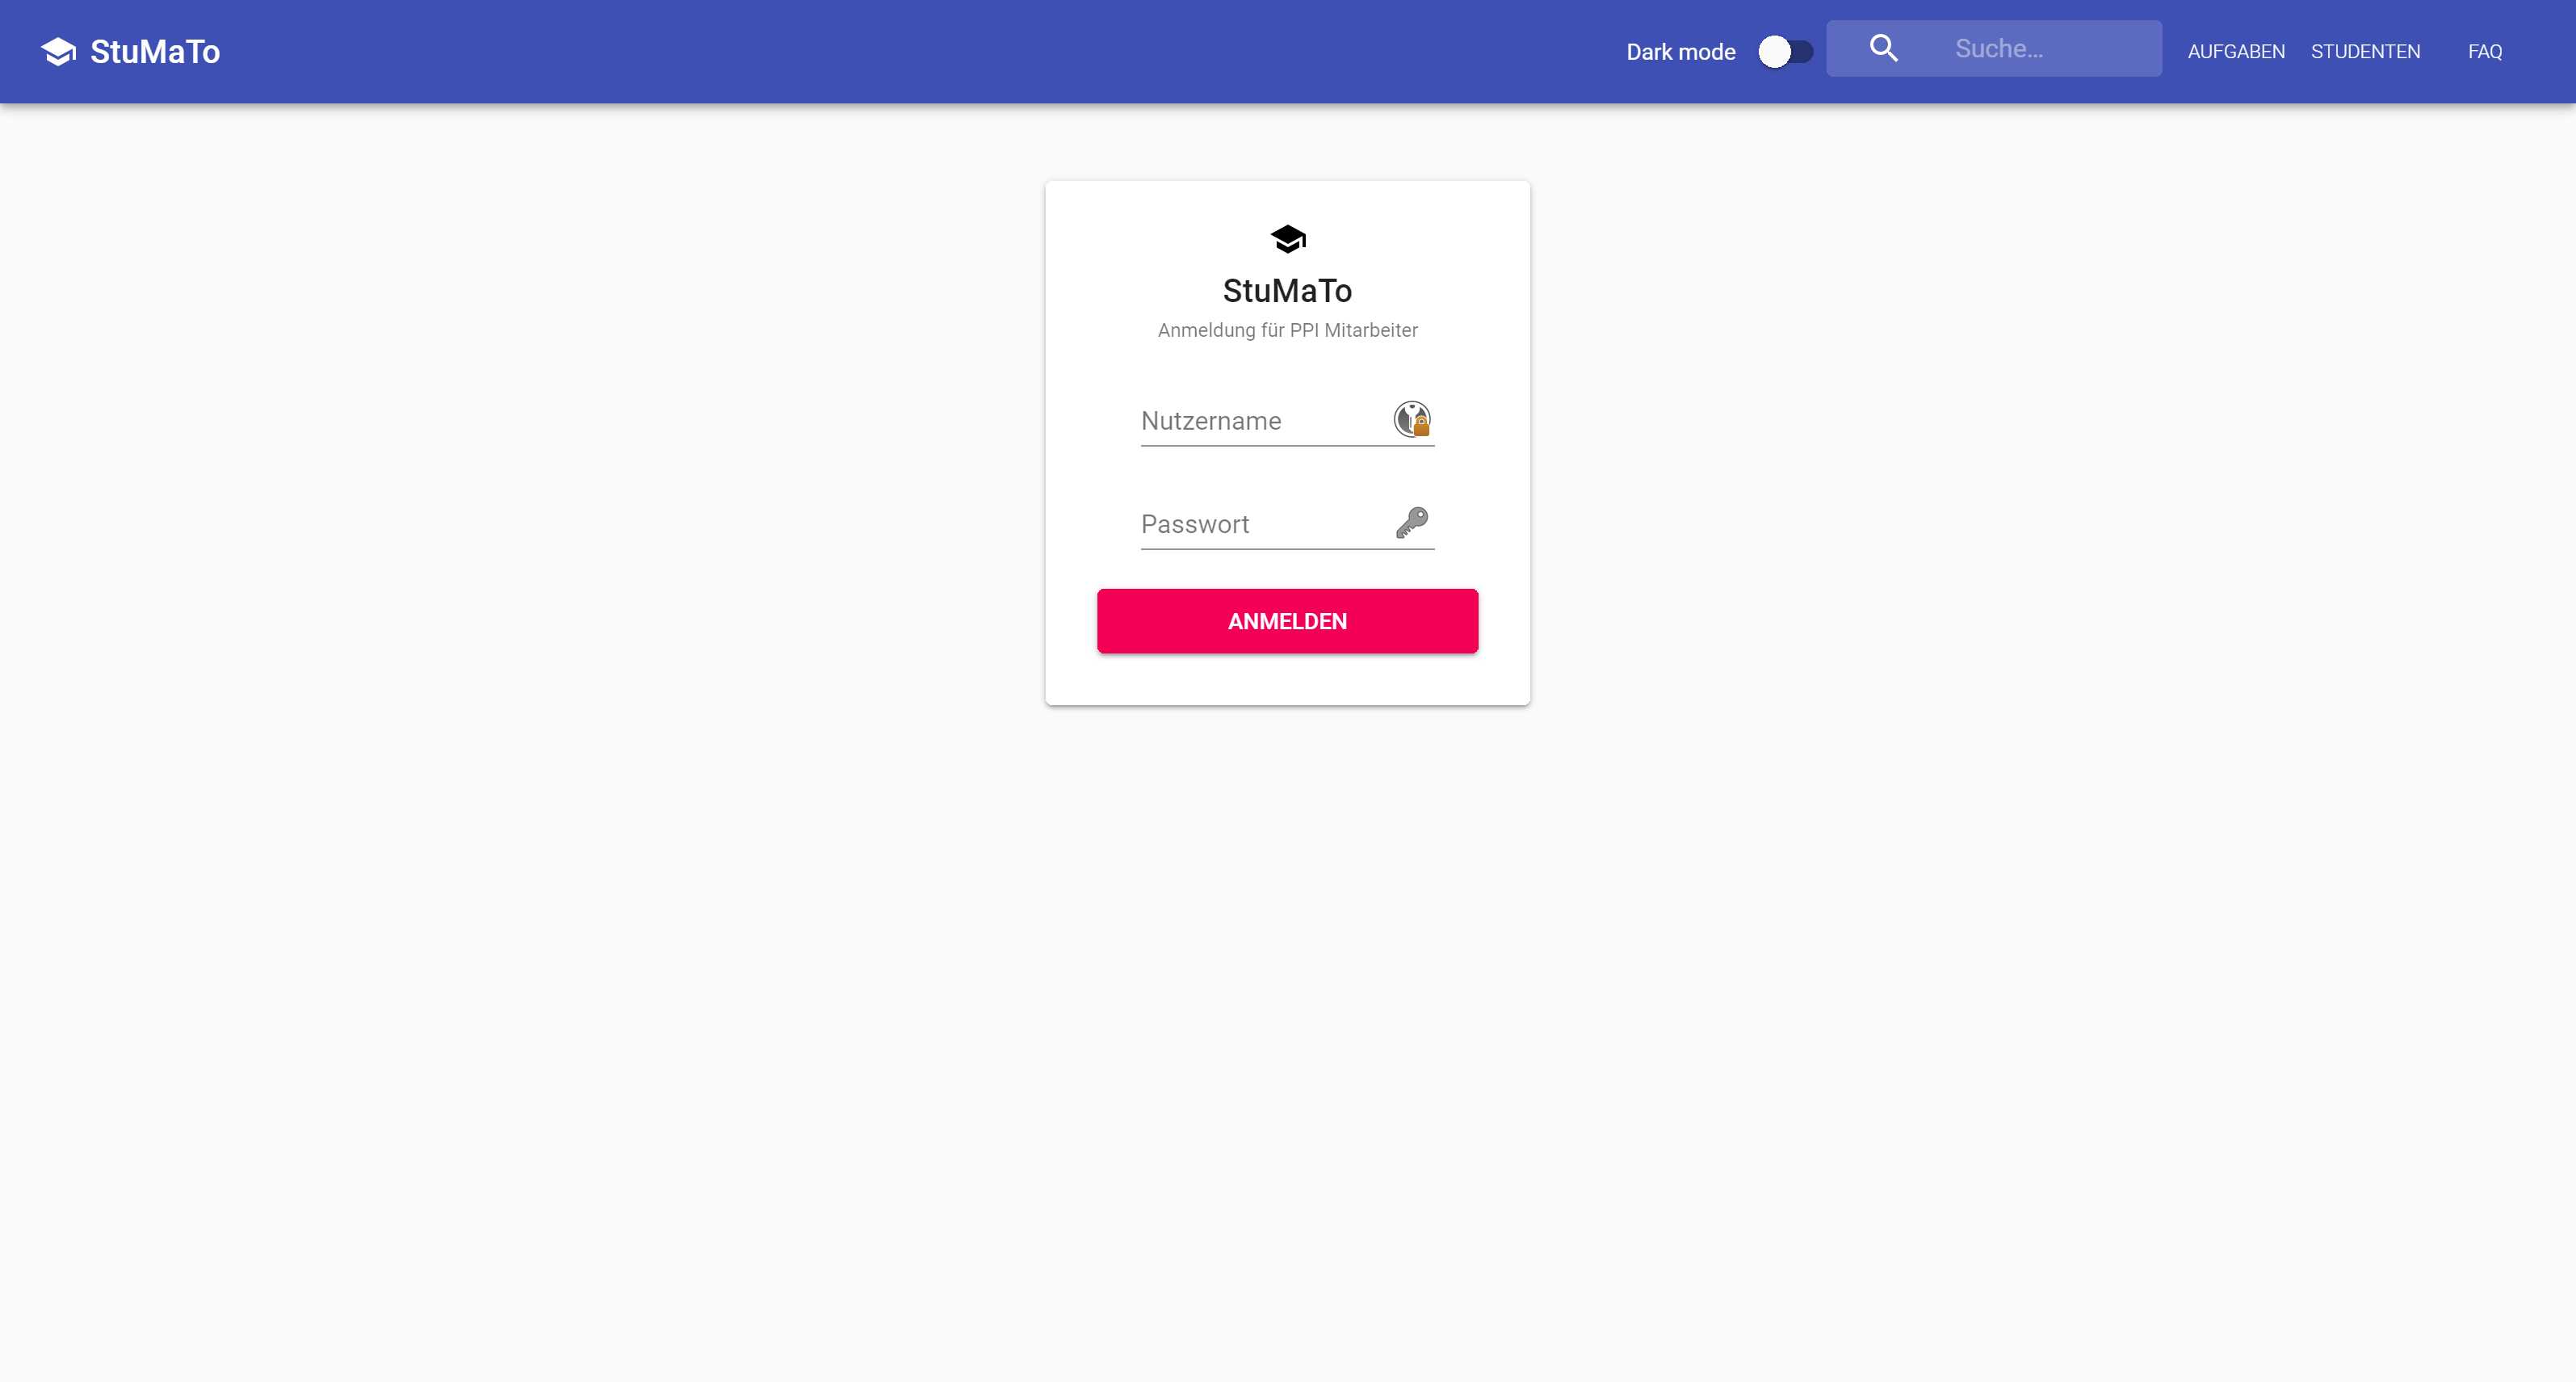
\includegraphics{./tex2pdf.-c803d322dfea80aa/9c5b8c473ccddcd0dab08da12cb1120c18a9138c.png}
\caption{Ansicht LOGIN}
\end{figure}

\begin{figure}
\centering
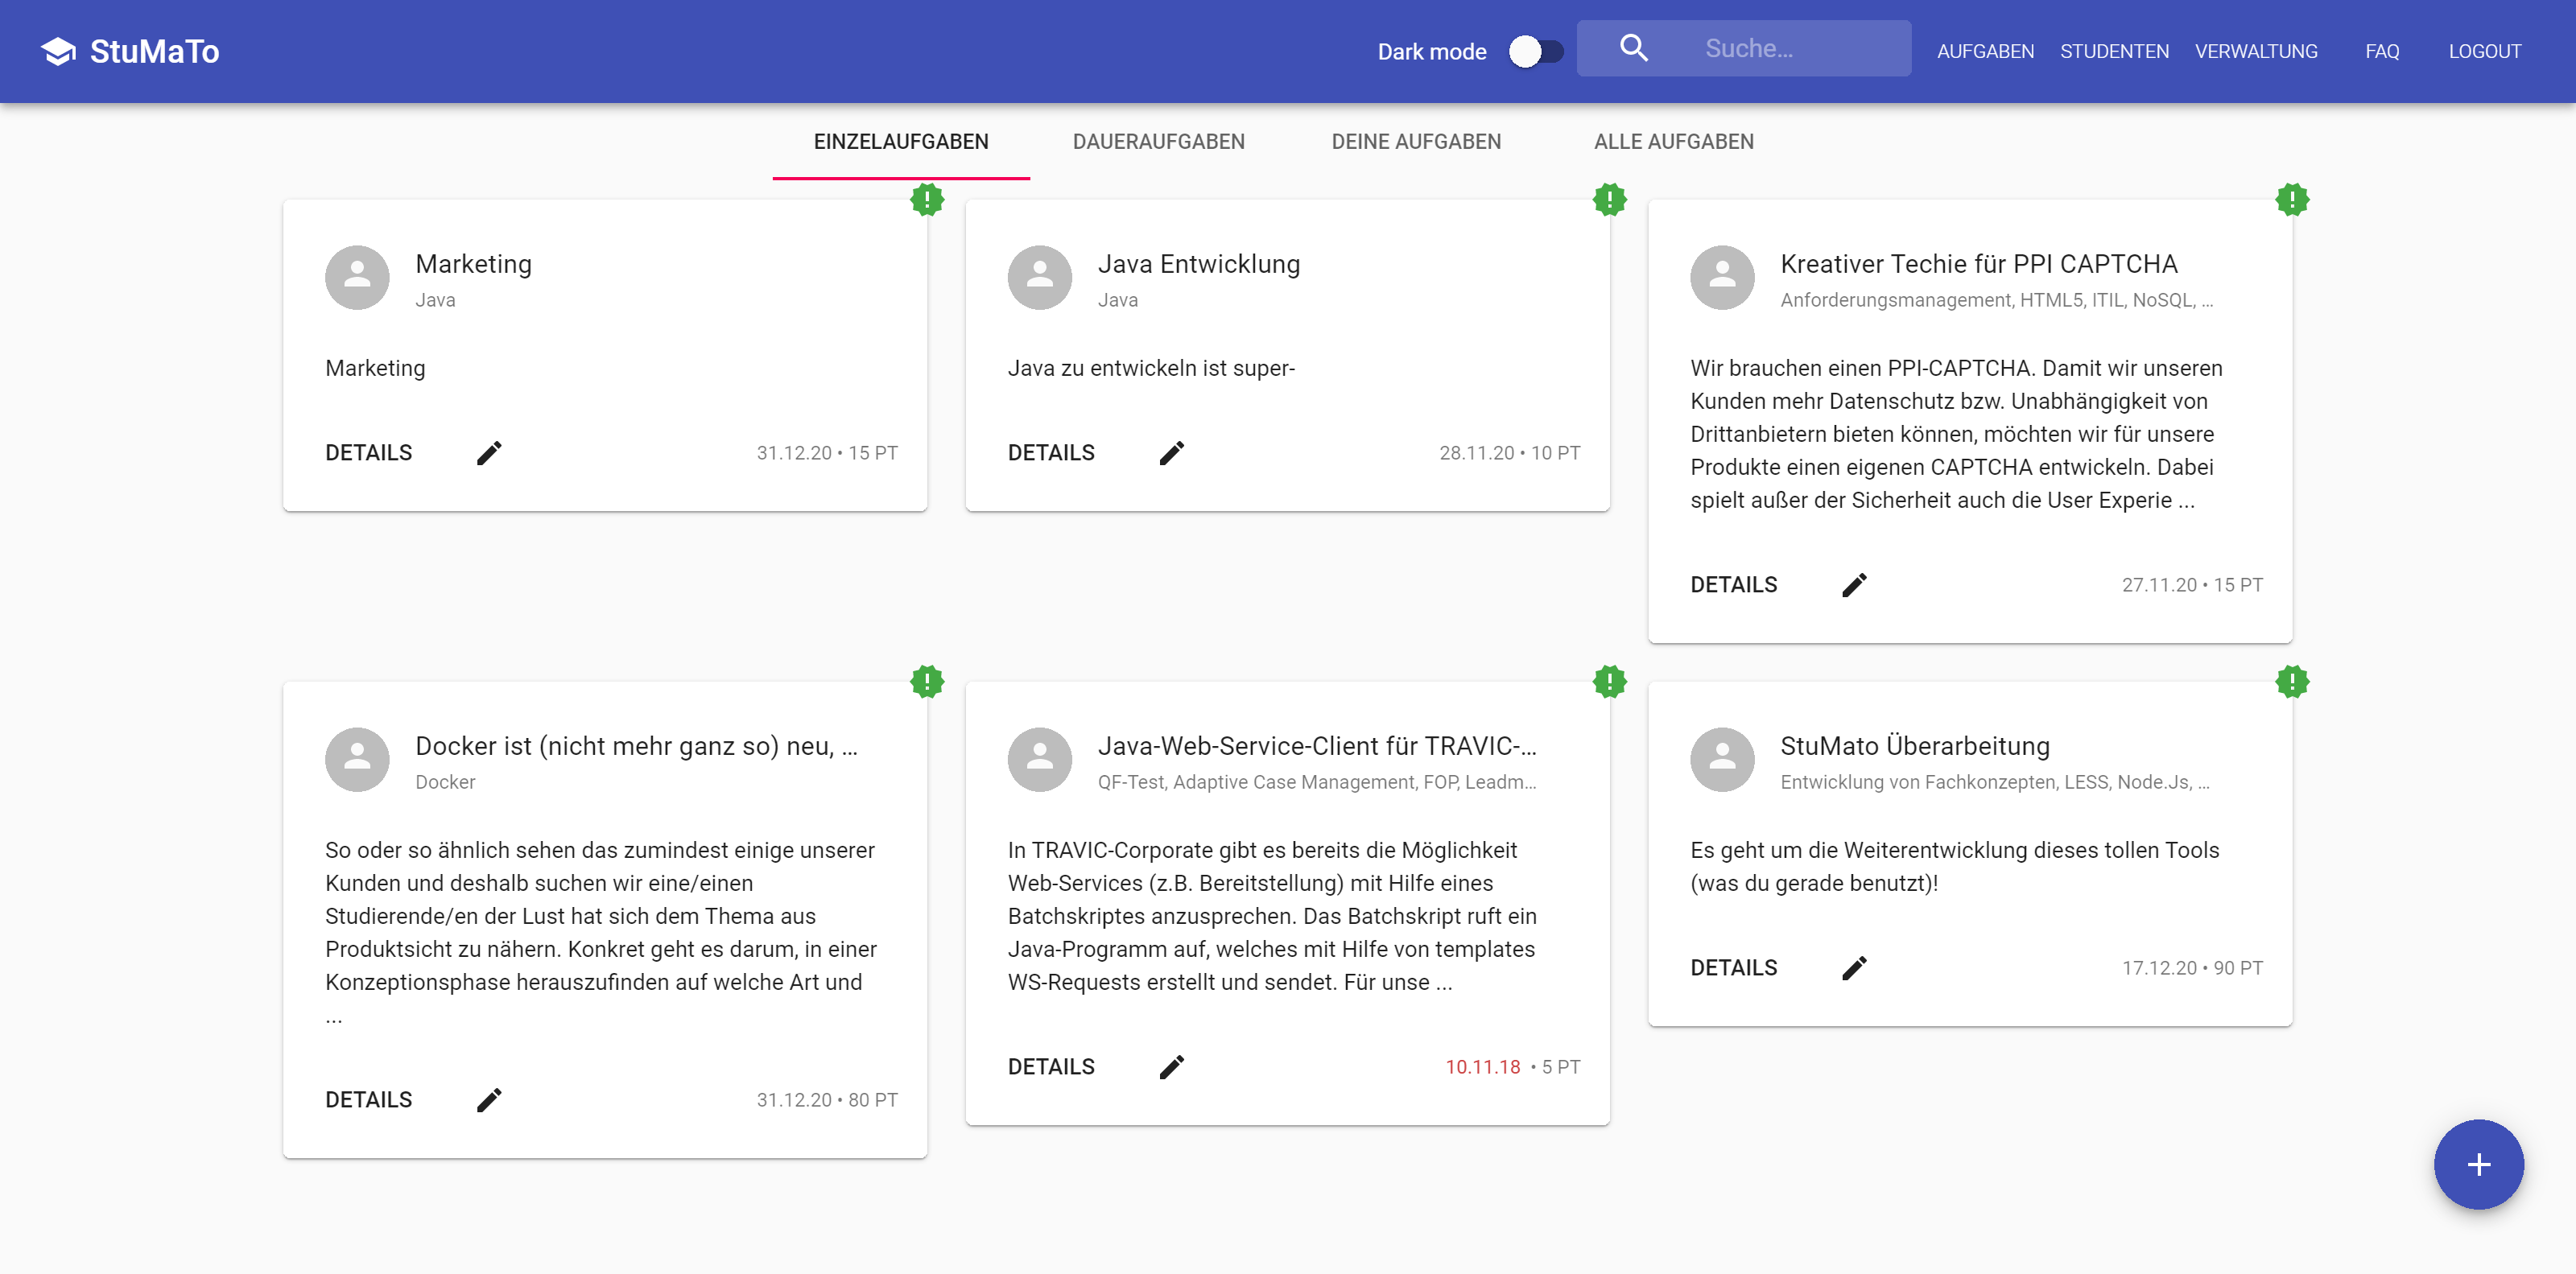
\includegraphics{./tex2pdf.-c803d322dfea80aa/f4cc5b5ab578b1b679cdbb7e8f0658dd5512d9e2.png}
\caption{Ansicht TASK.SINGLE}
\end{figure}

\begin{figure}
\centering
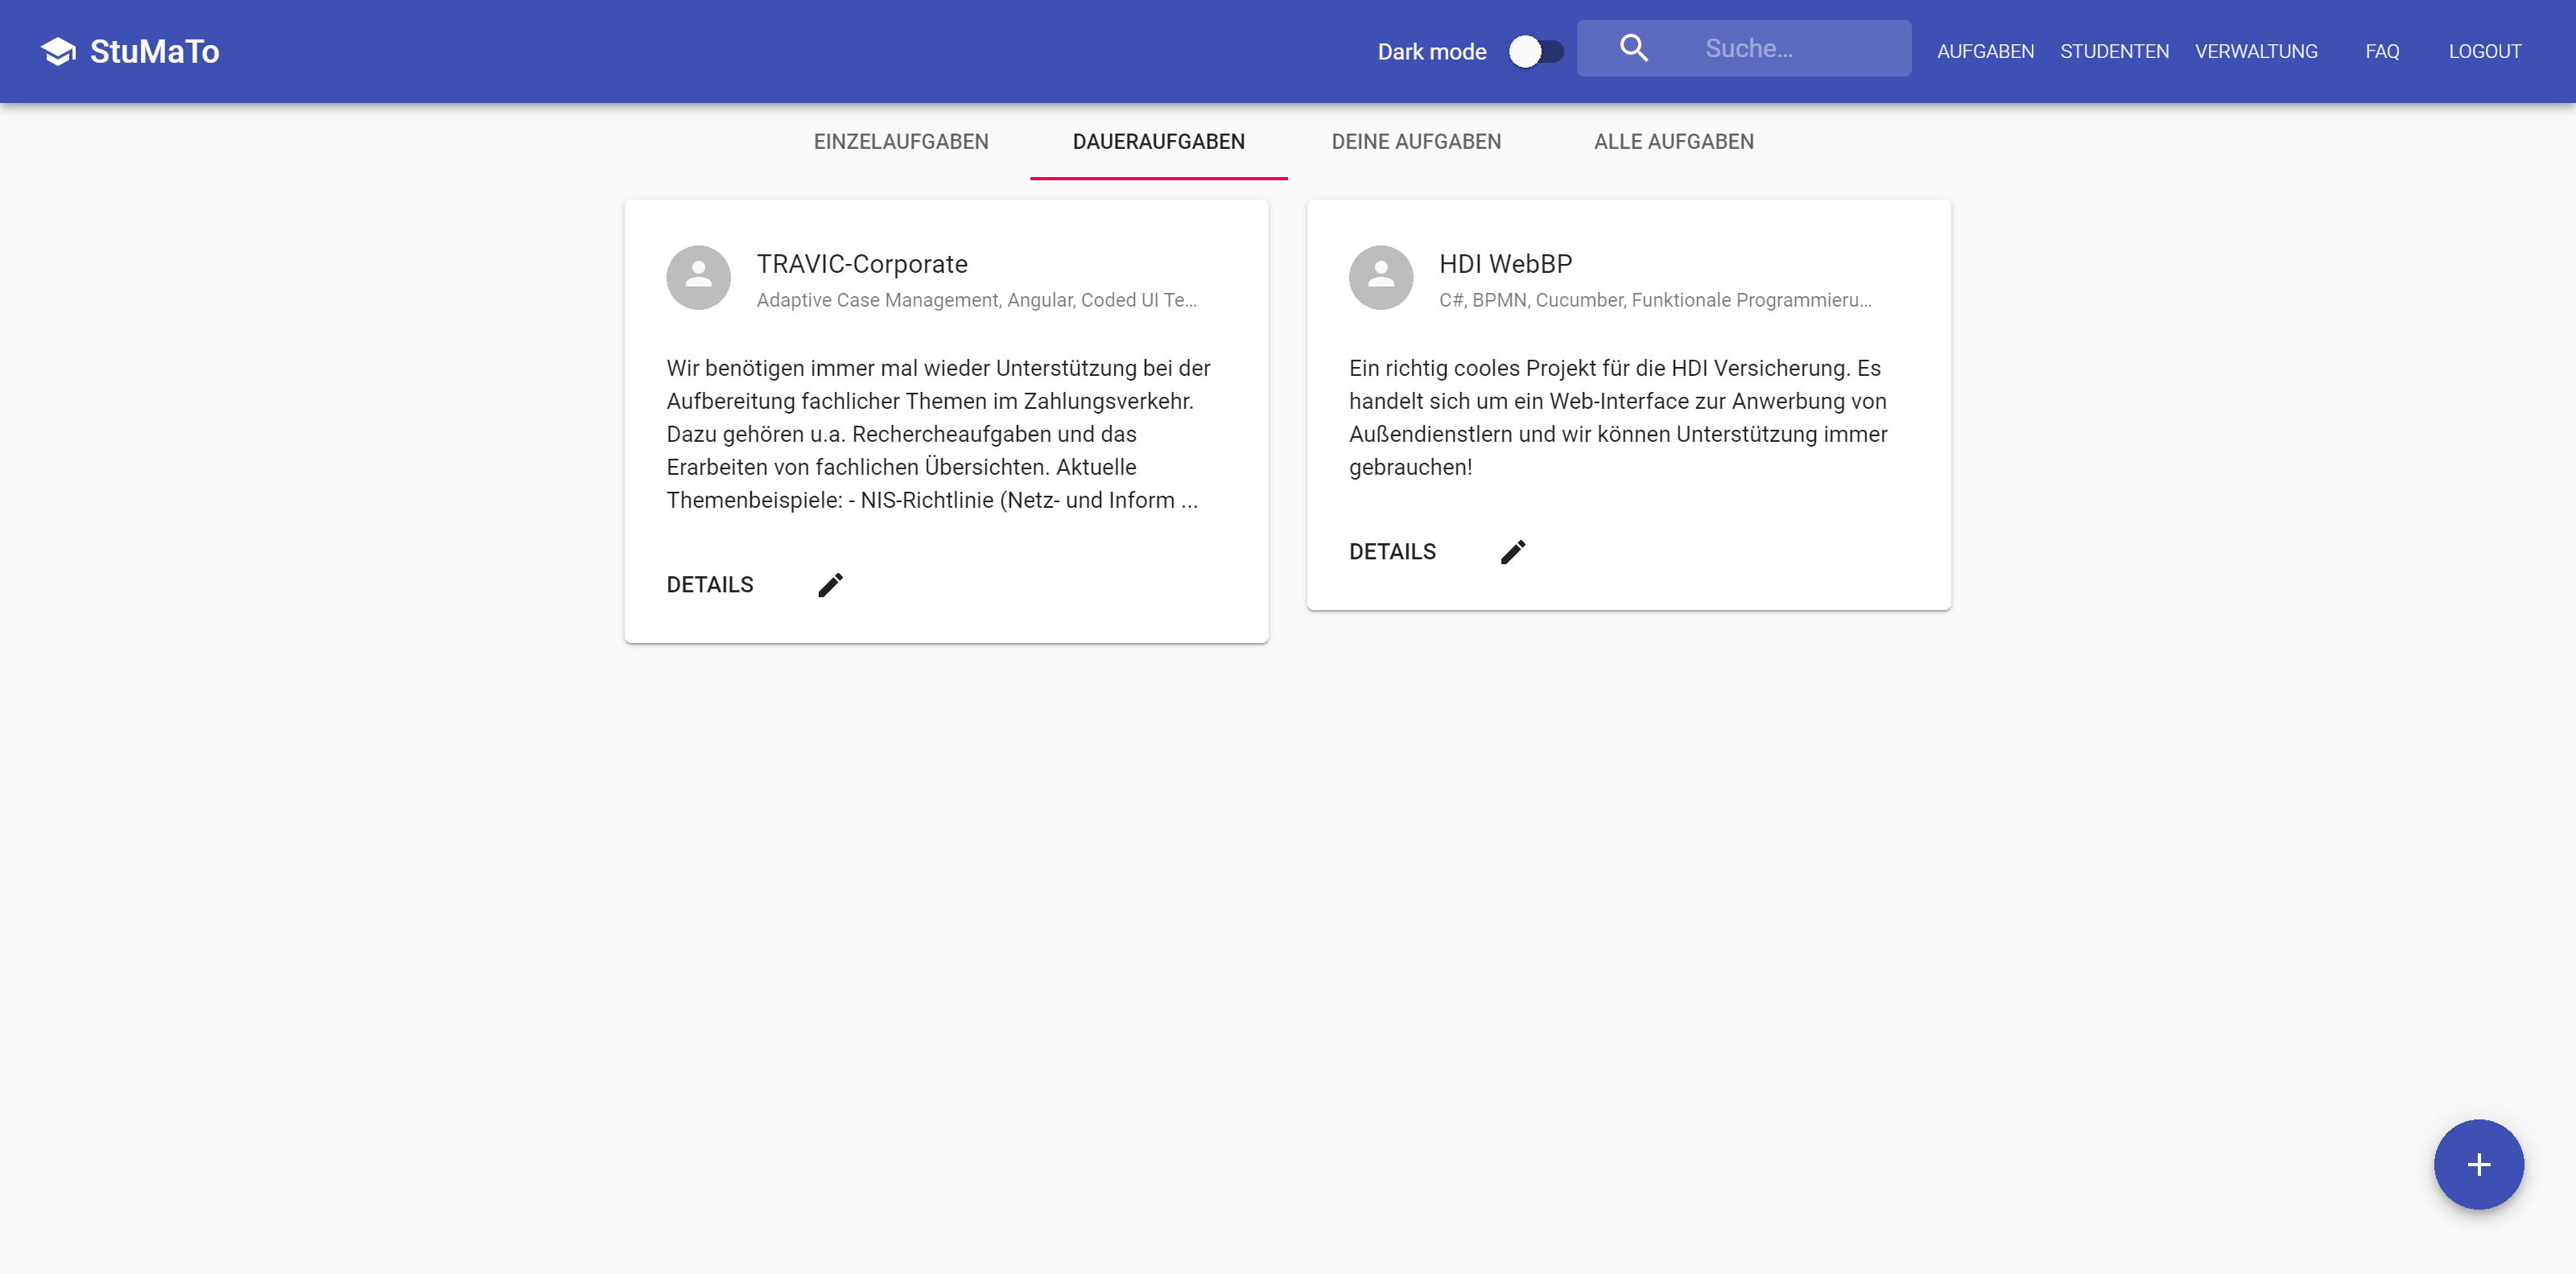
\includegraphics{./tex2pdf.-c803d322dfea80aa/d3c6a43d479a4c11a45a24bd6d652630f2dfa188.png}
\caption{Ansicht TASK.PERM}
\end{figure}

\begin{figure}
\centering
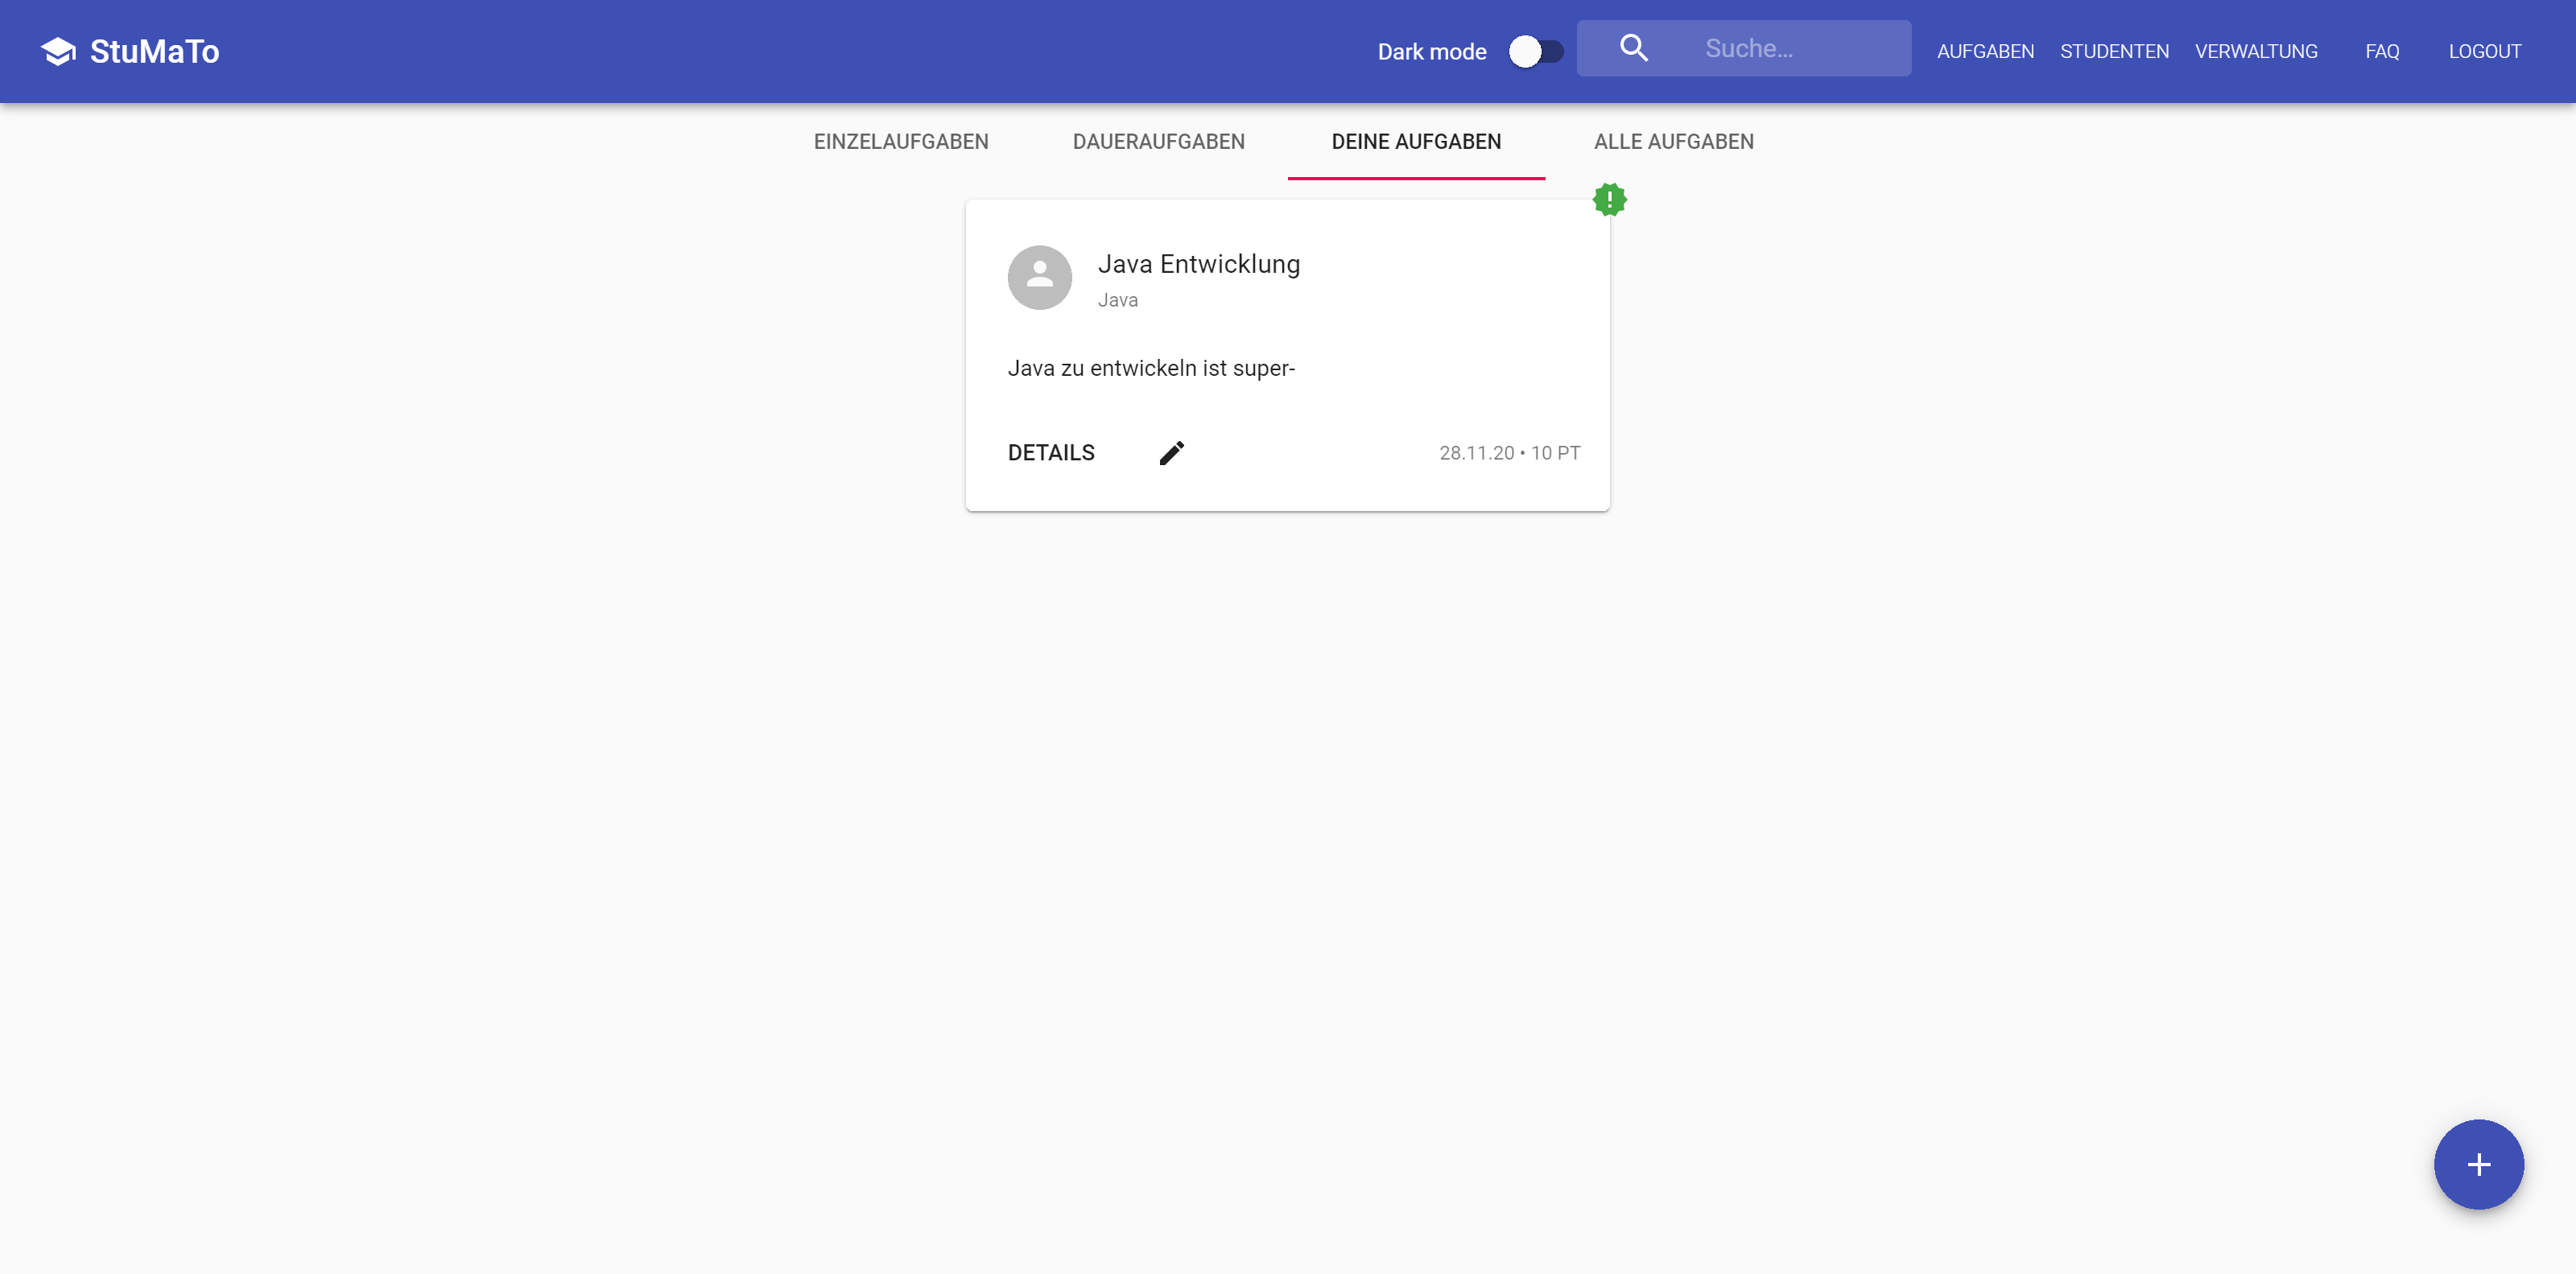
\includegraphics{./tex2pdf.-c803d322dfea80aa/108f3c537d8035b8bdc8a1058ba8f82610771530.png}
\caption{Ansicht TASK.YOUR}
\end{figure}

\begin{figure}
\centering
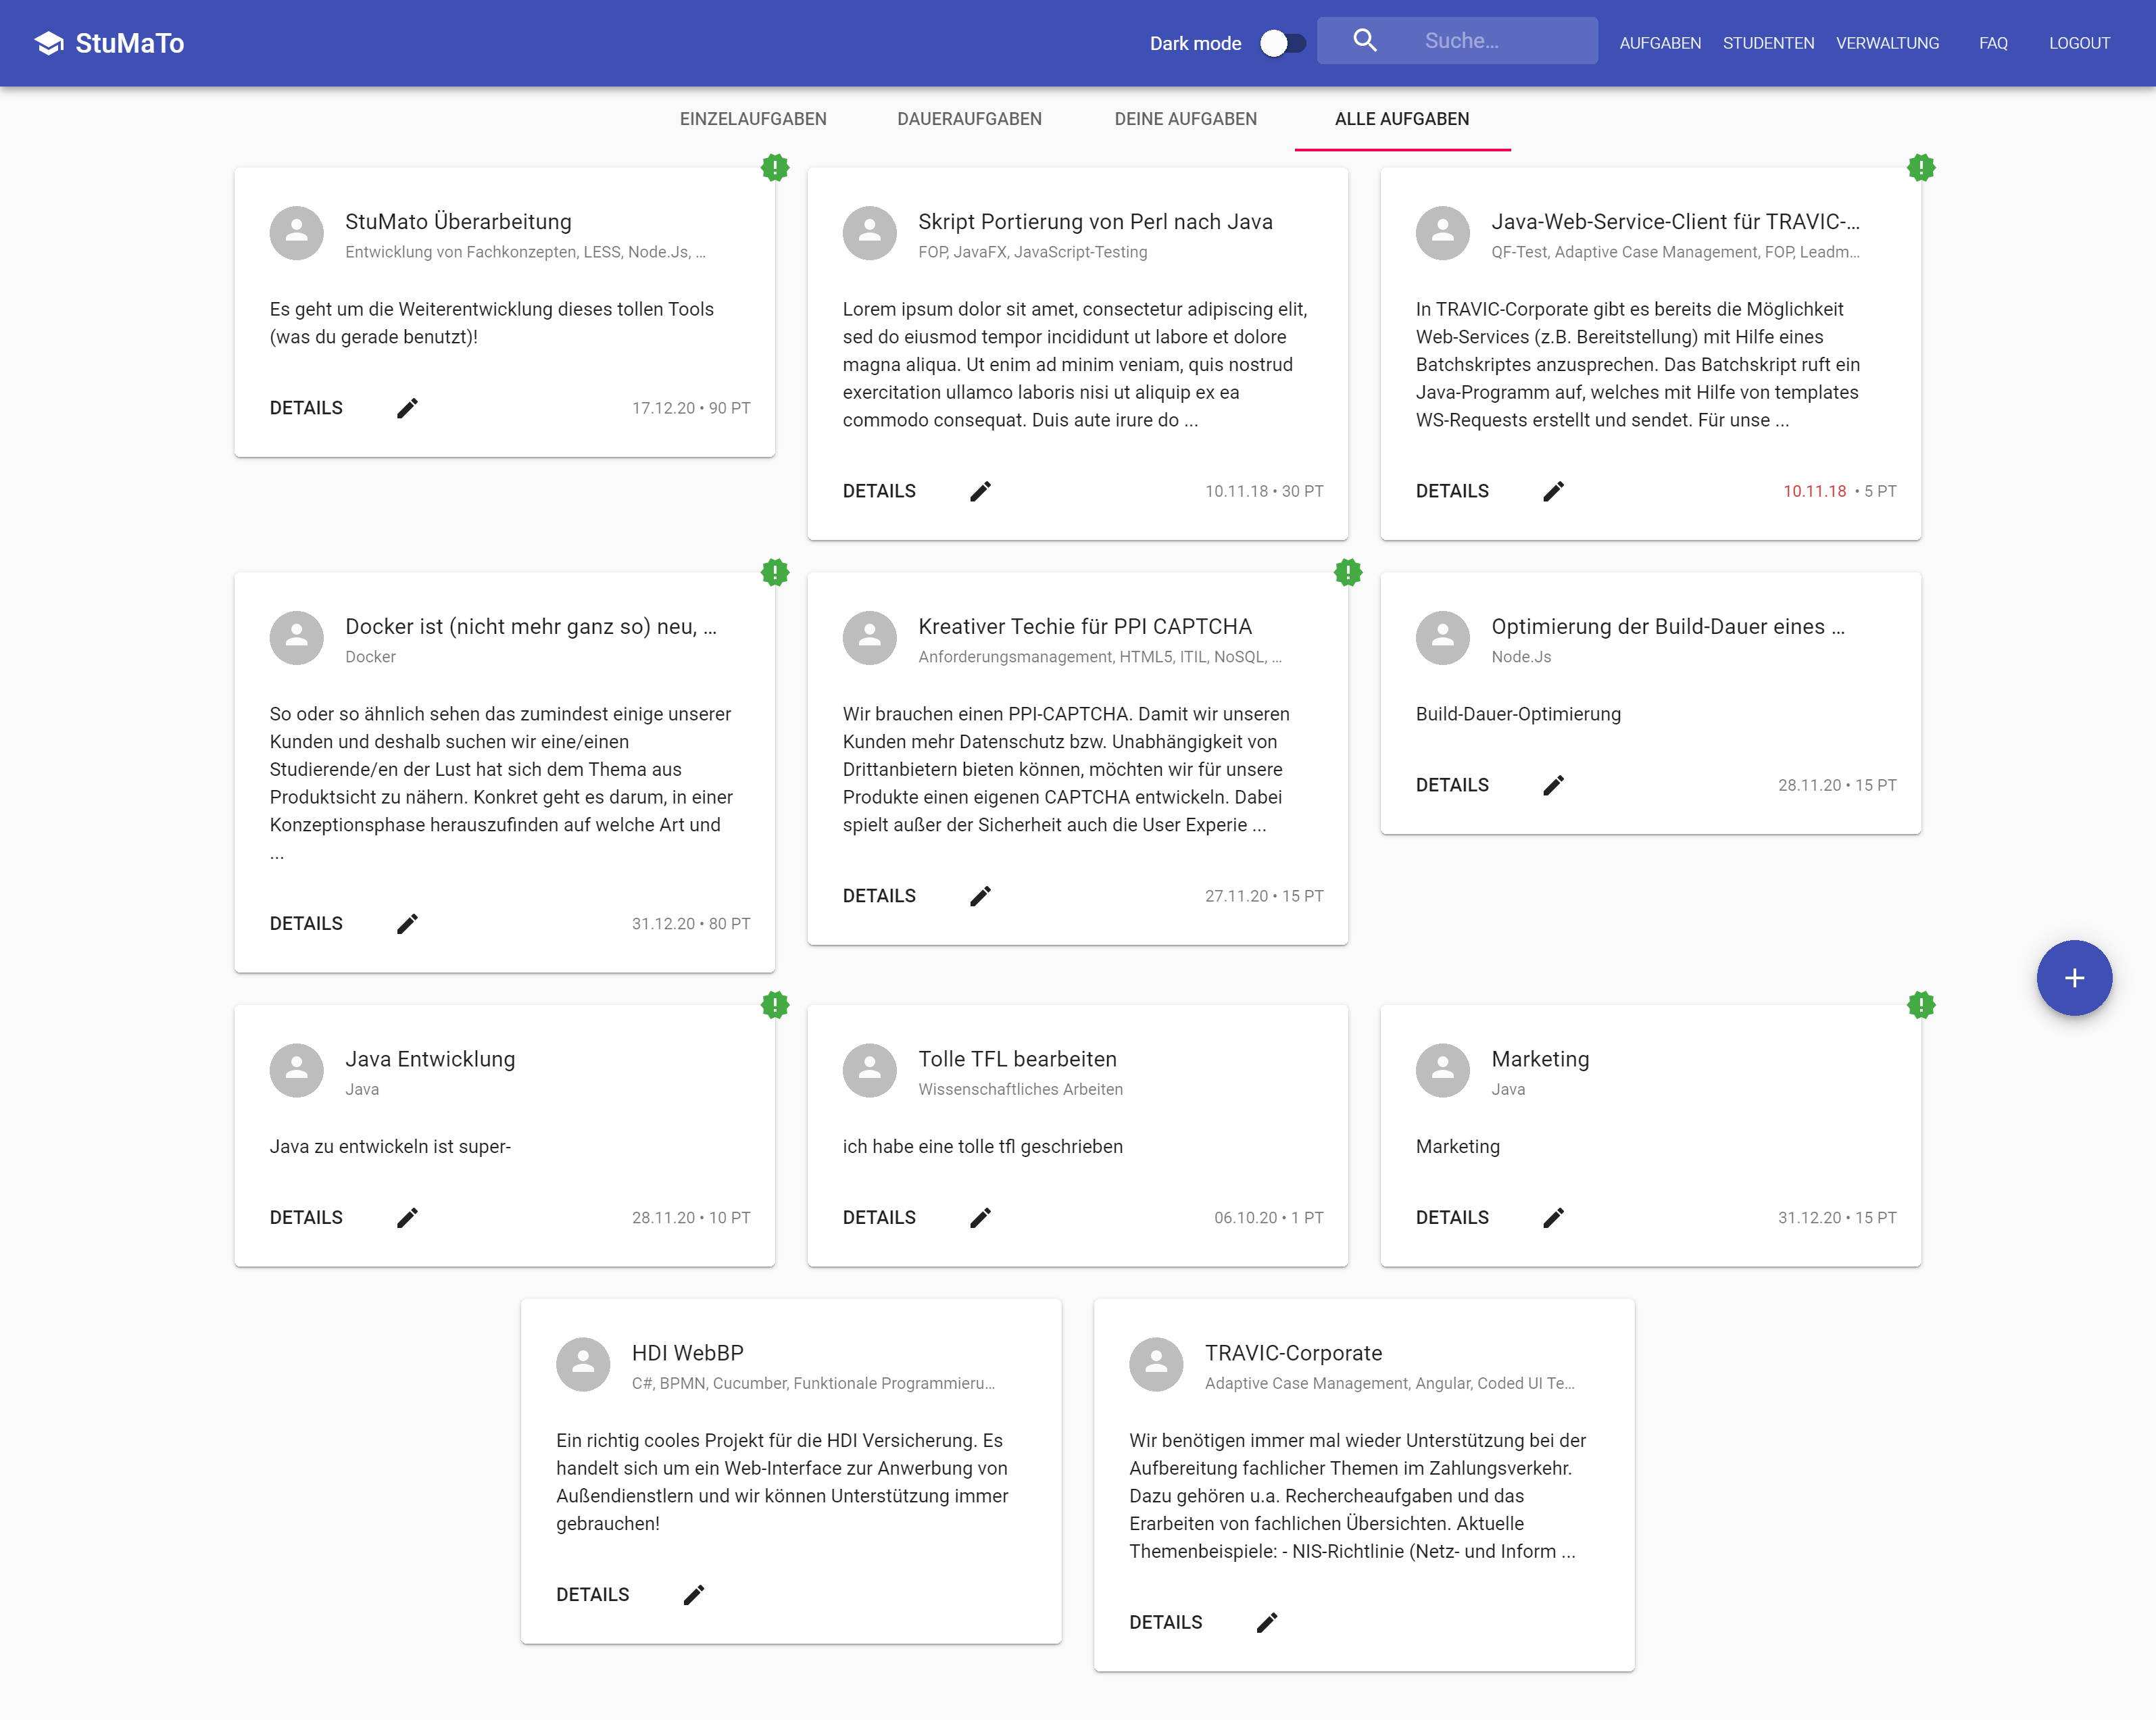
\includegraphics{./tex2pdf.-c803d322dfea80aa/da9ee686dc2d8ad97ac31e5253caf99016a4e3f5.png}
\caption{Ansicht TASK.ALL}
\end{figure}

\begin{figure}
\centering
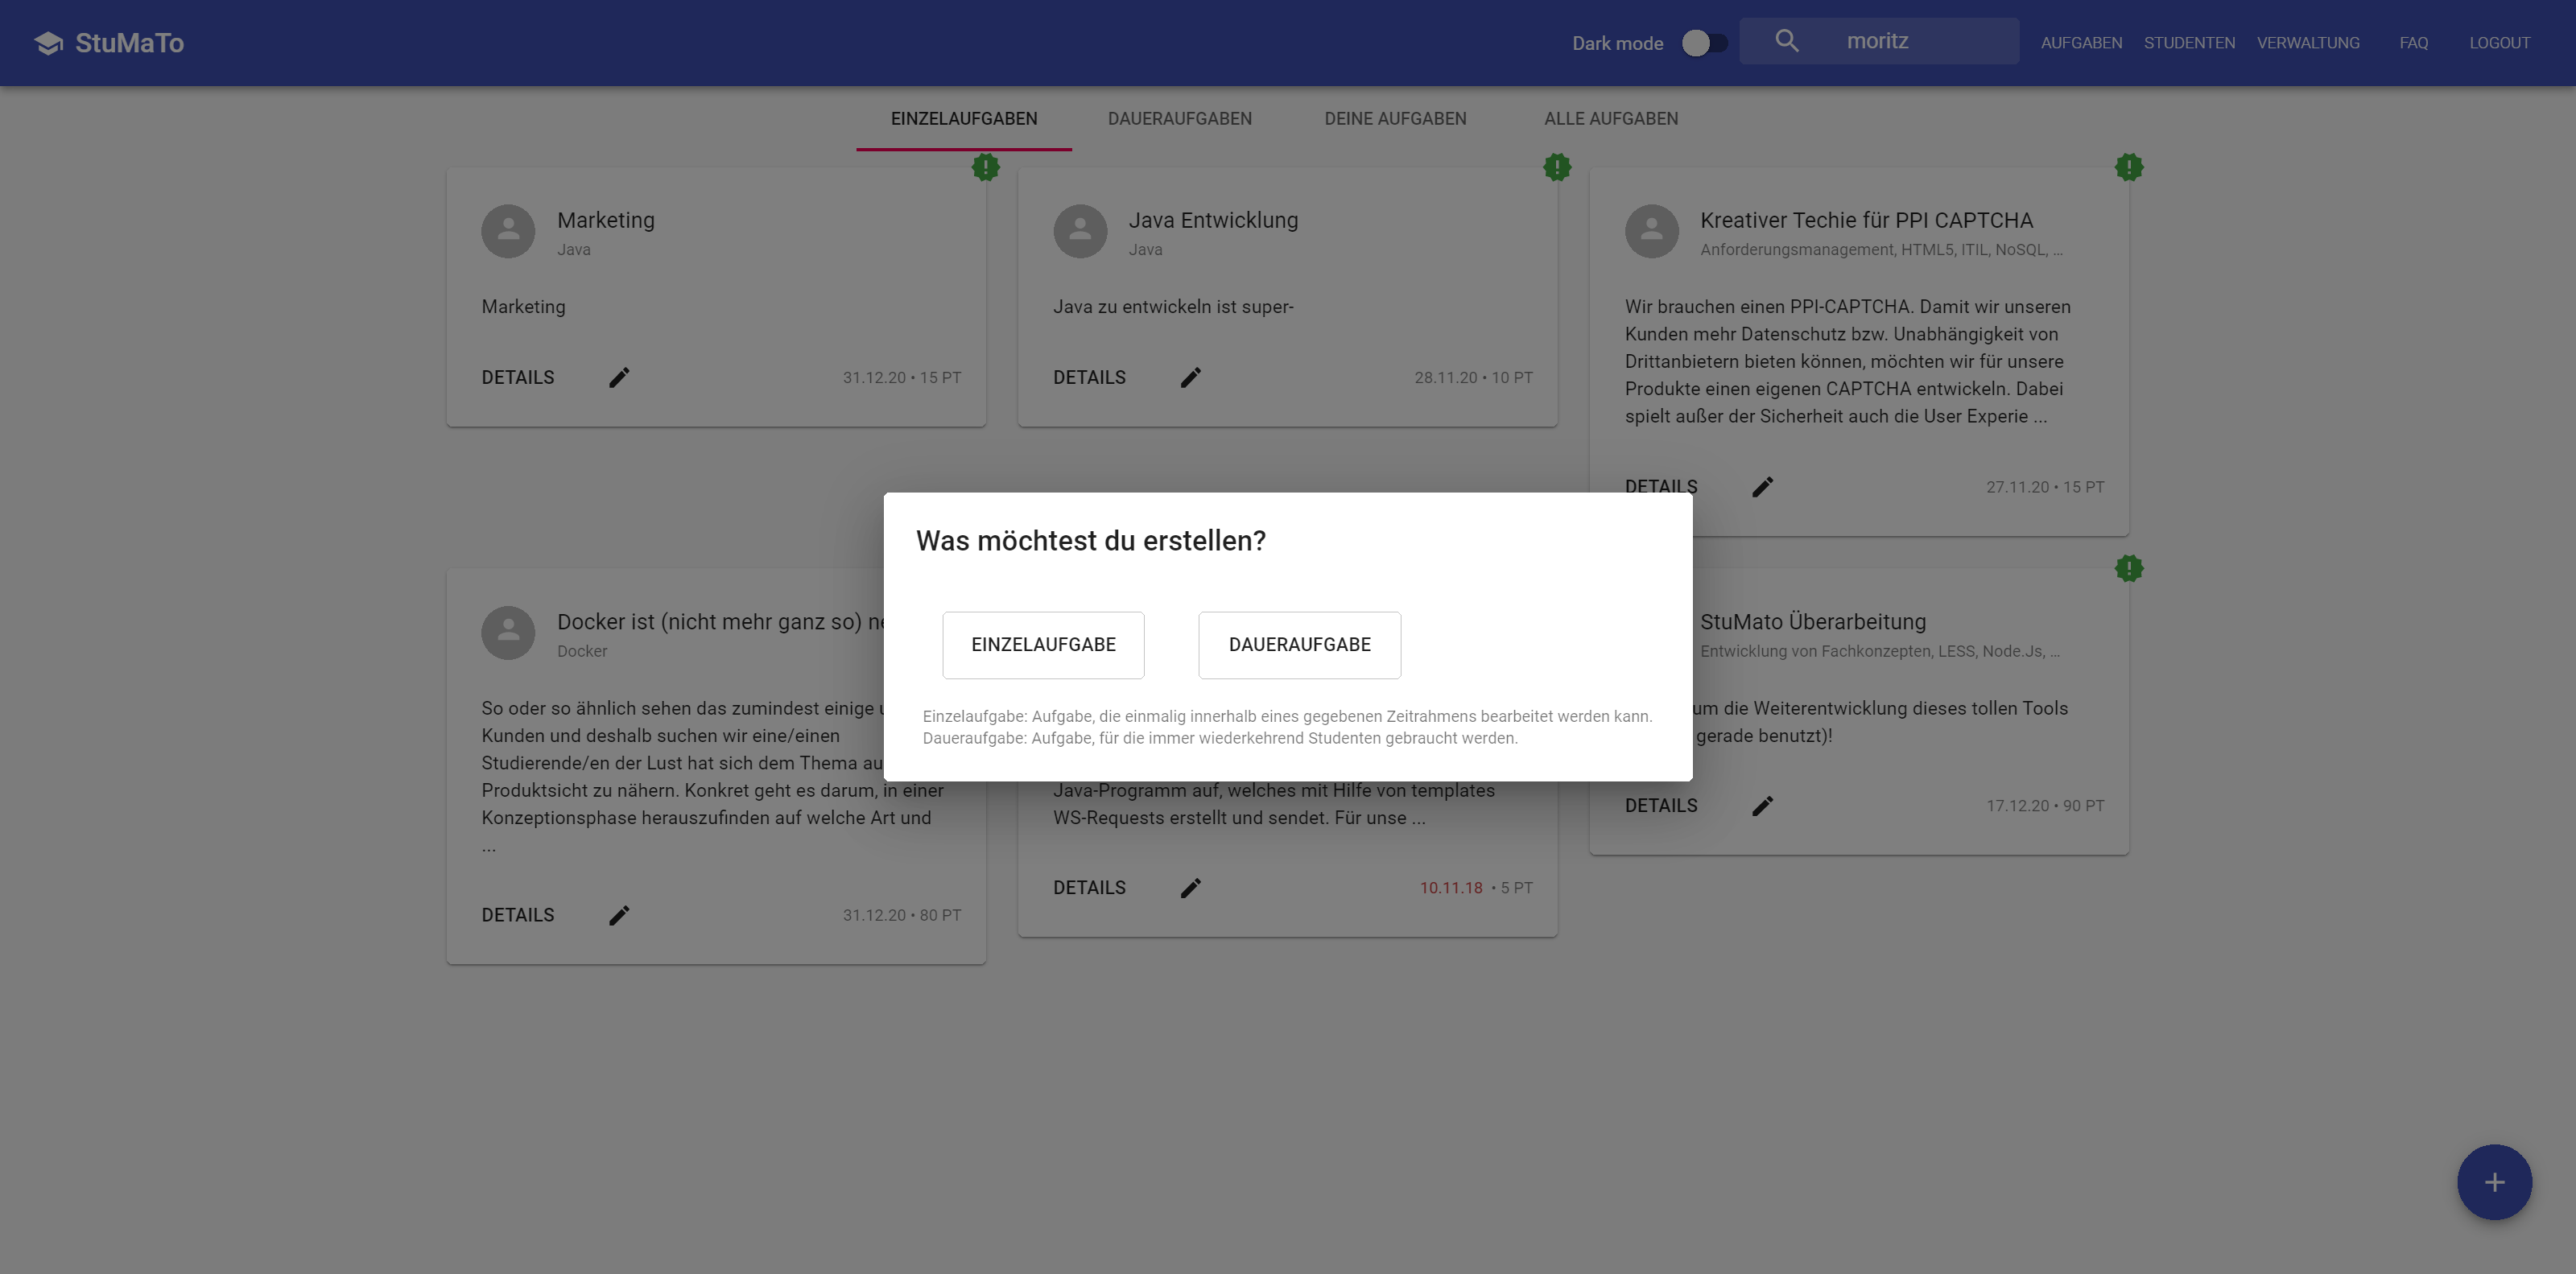
\includegraphics{./tex2pdf.-c803d322dfea80aa/303dcfe459fd3b8446fc3094f7aa678a2a72eef0.png}
\caption{Ansicht TASK.NEW}
\end{figure}

\begin{figure}
\centering
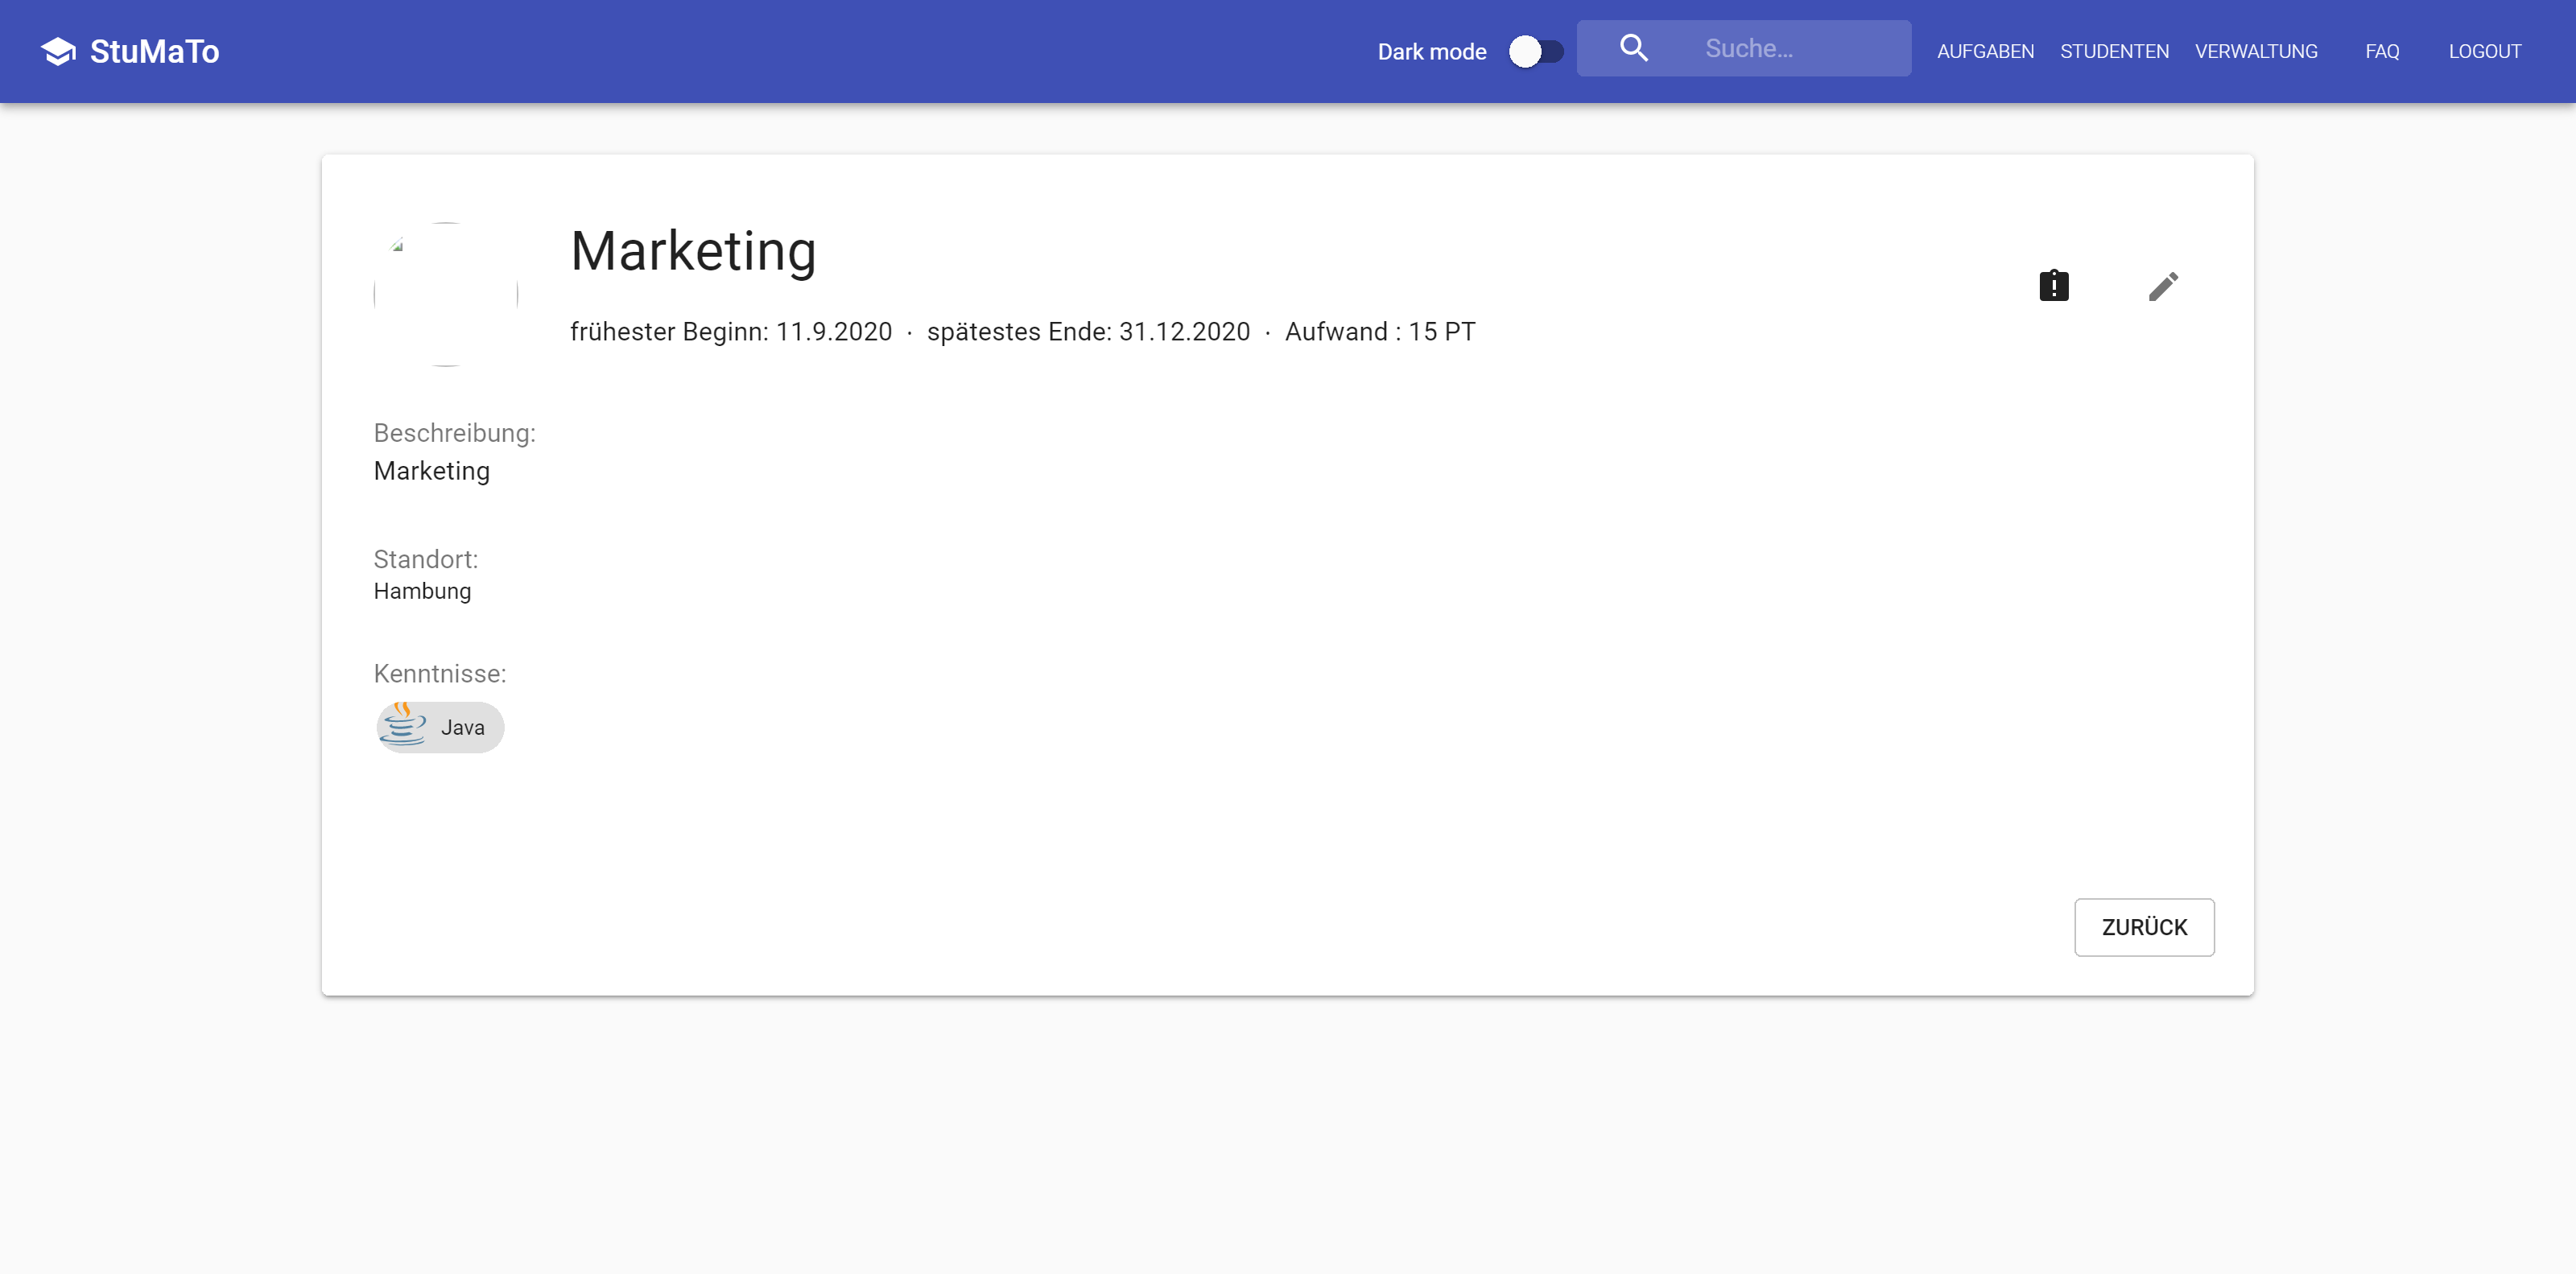
\includegraphics{./tex2pdf.-c803d322dfea80aa/7908951722dfee3f634678faf93fa21ee7f6c477.png}
\caption{Ansicht TASK.VIEW}
\end{figure}

\begin{figure}
\centering
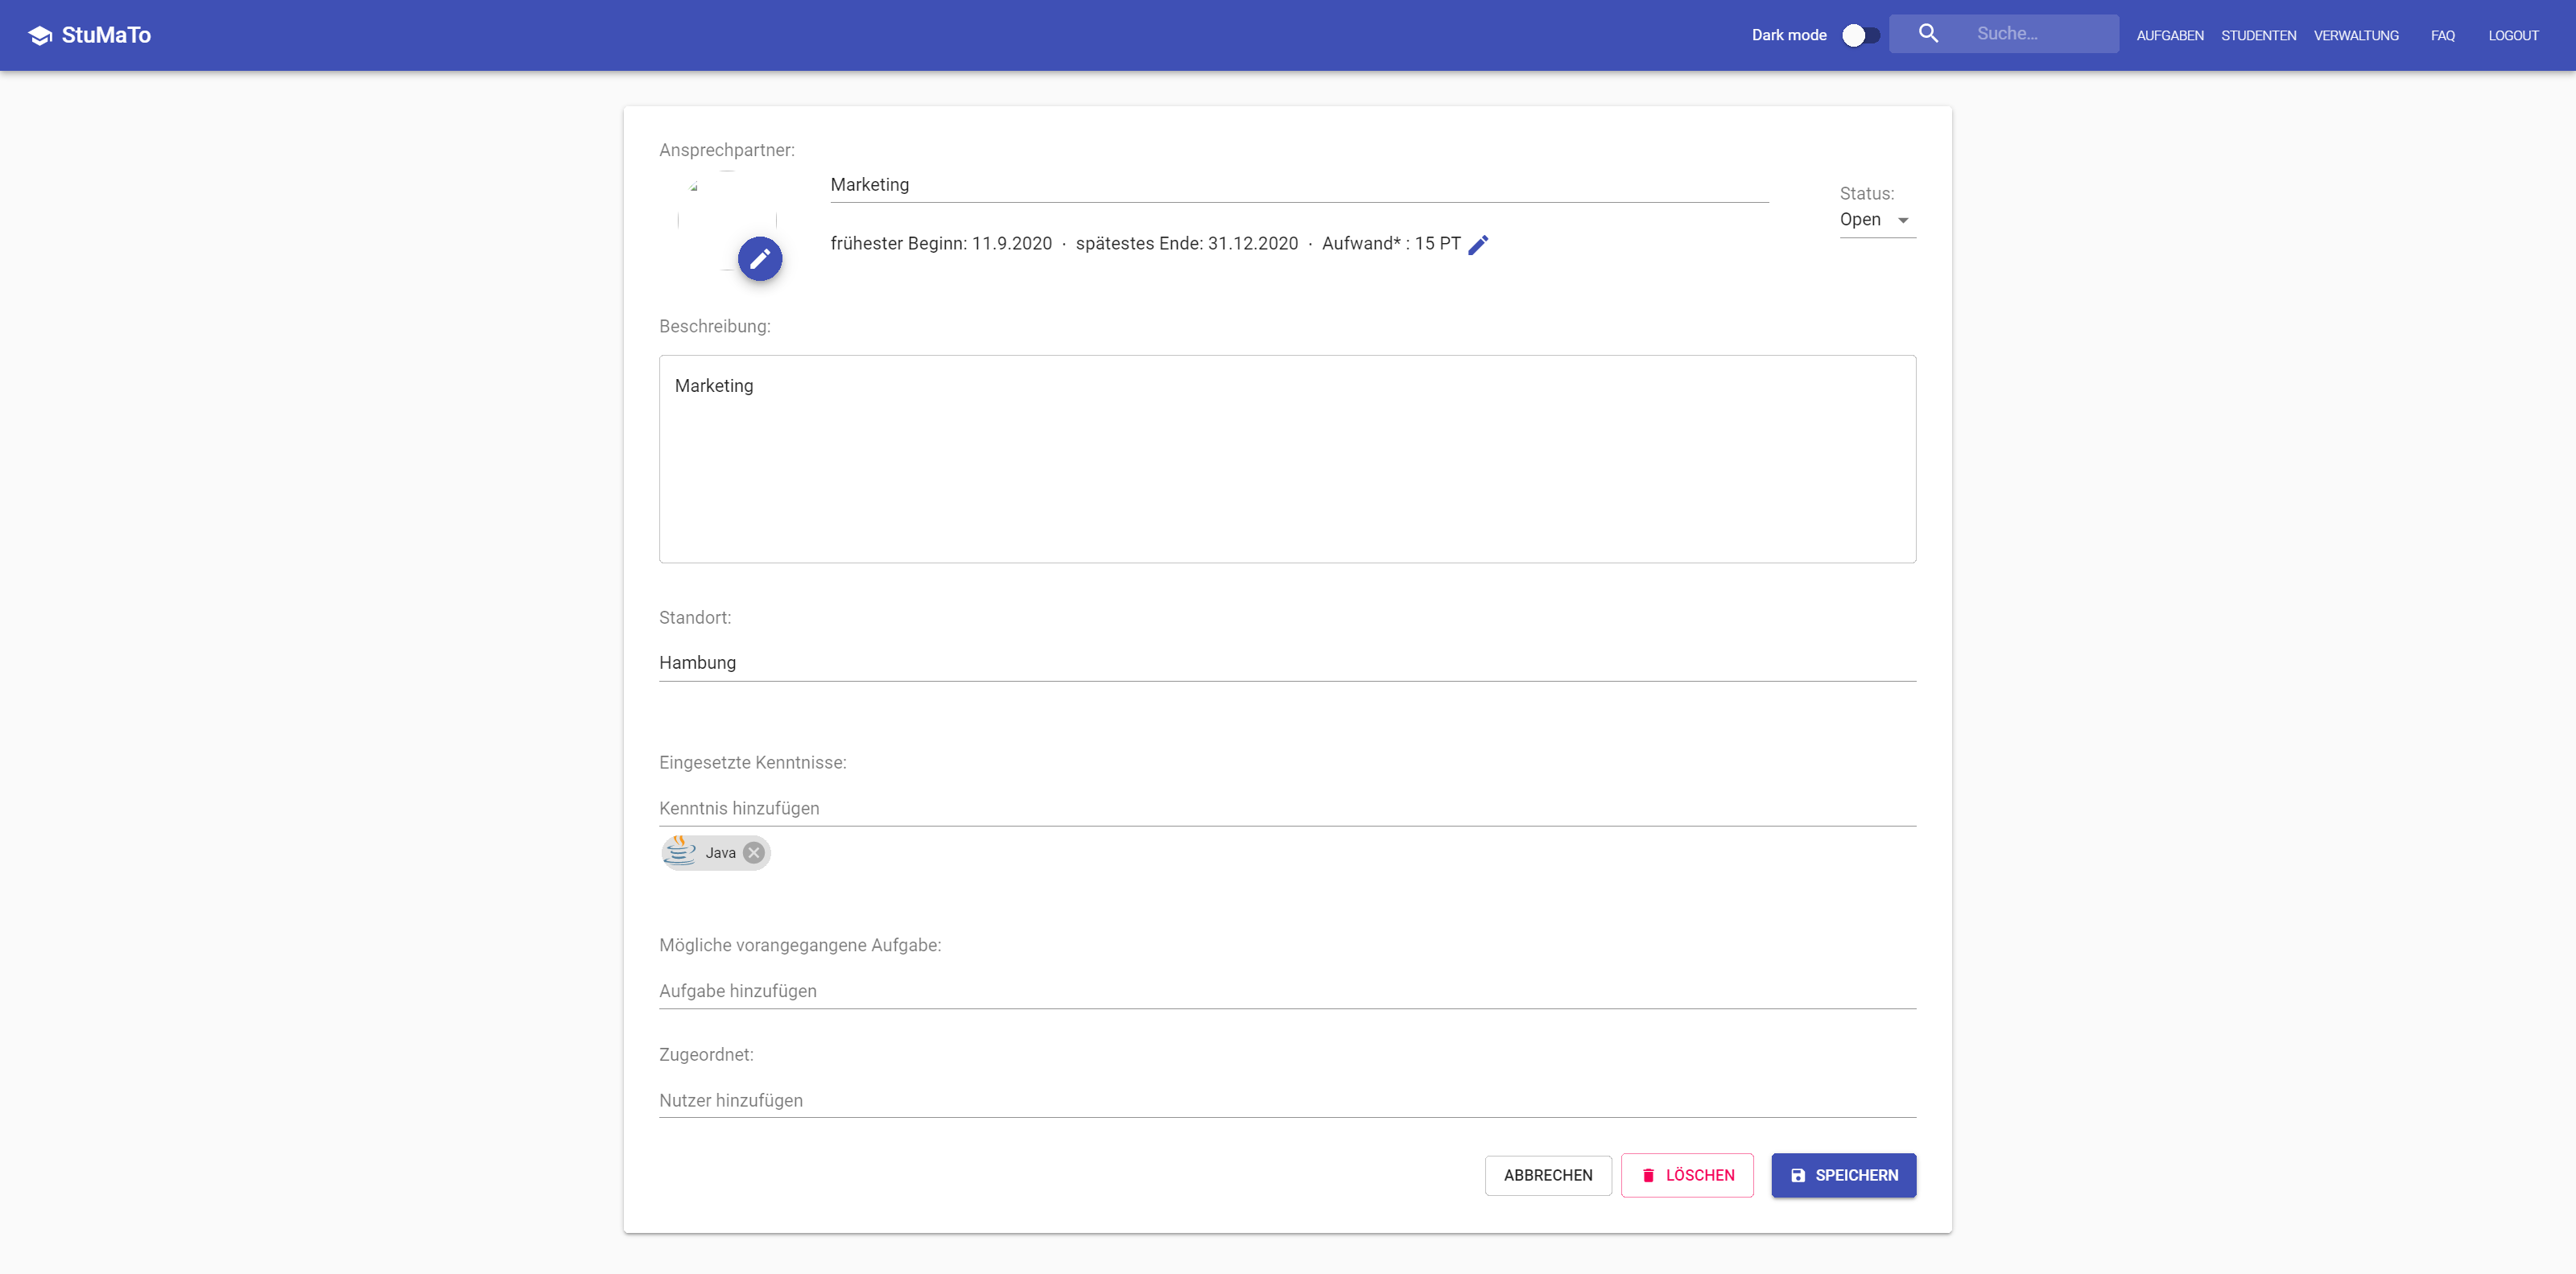
\includegraphics{./tex2pdf.-c803d322dfea80aa/1526445399f73b404890c7f4a0cca5189b06eb12.png}
\caption{Ansicht TASK.EDIT}
\end{figure}

\begin{figure}
\centering
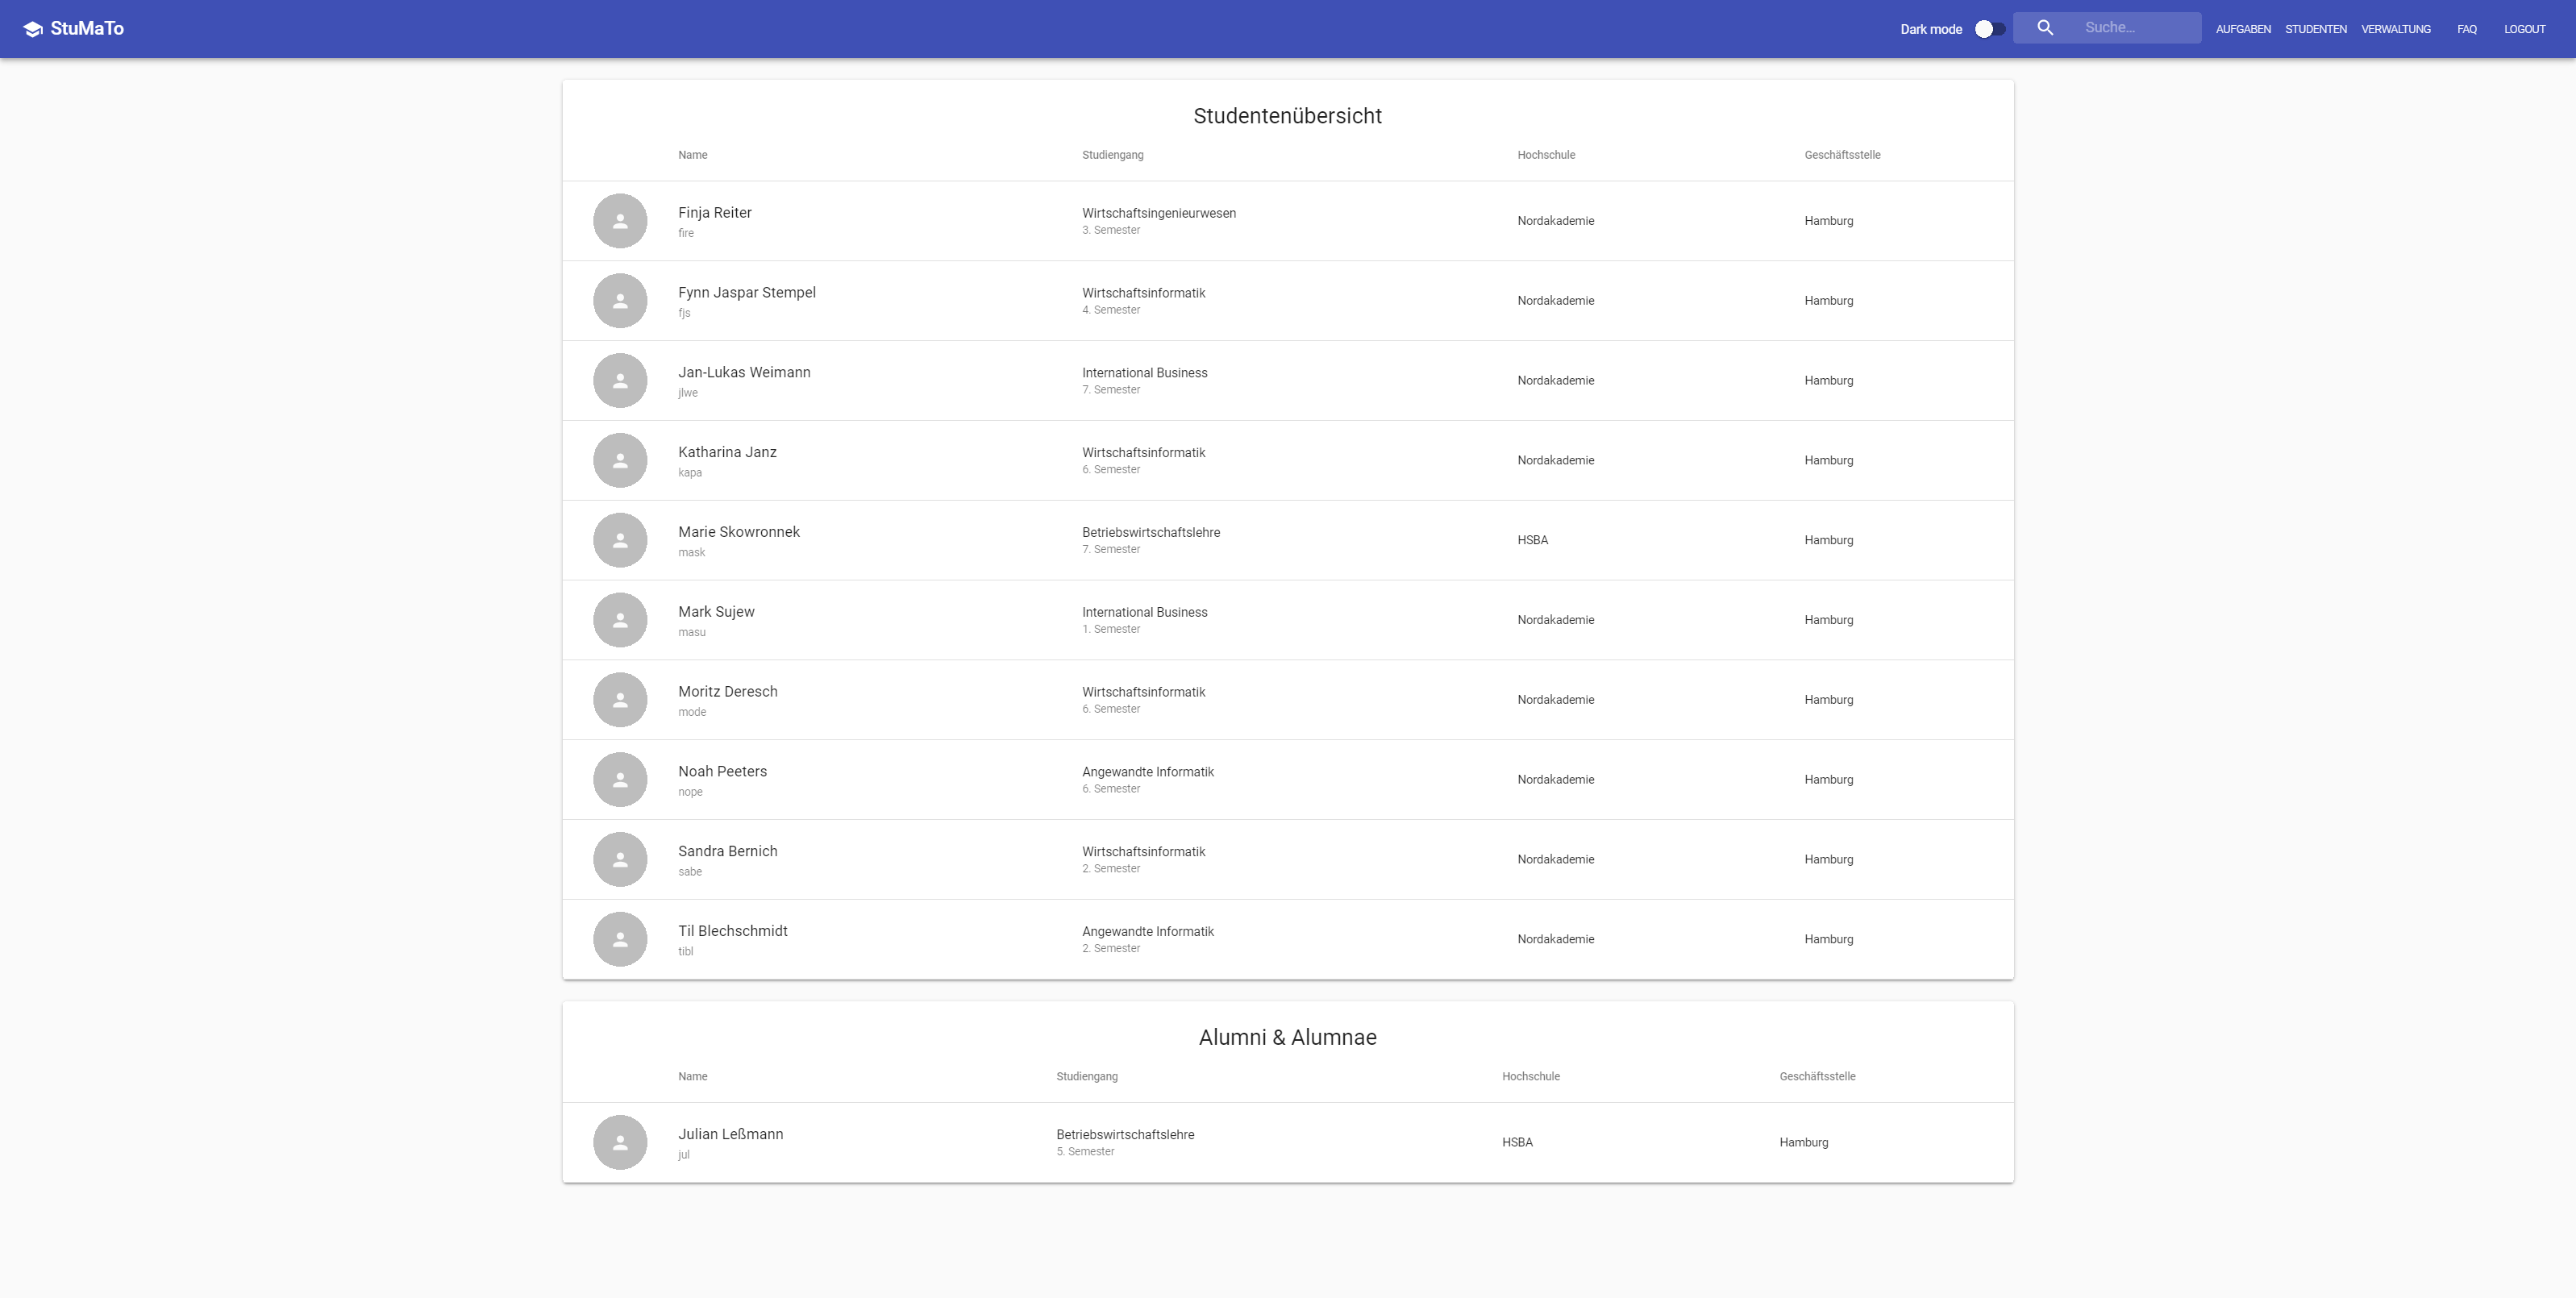
\includegraphics{./tex2pdf.-c803d322dfea80aa/14347ebd1a68ae90215eaa0204da9facc81485bd.png}
\caption{Ansicht STUDENT.LIST}
\end{figure}

\begin{figure}
\centering
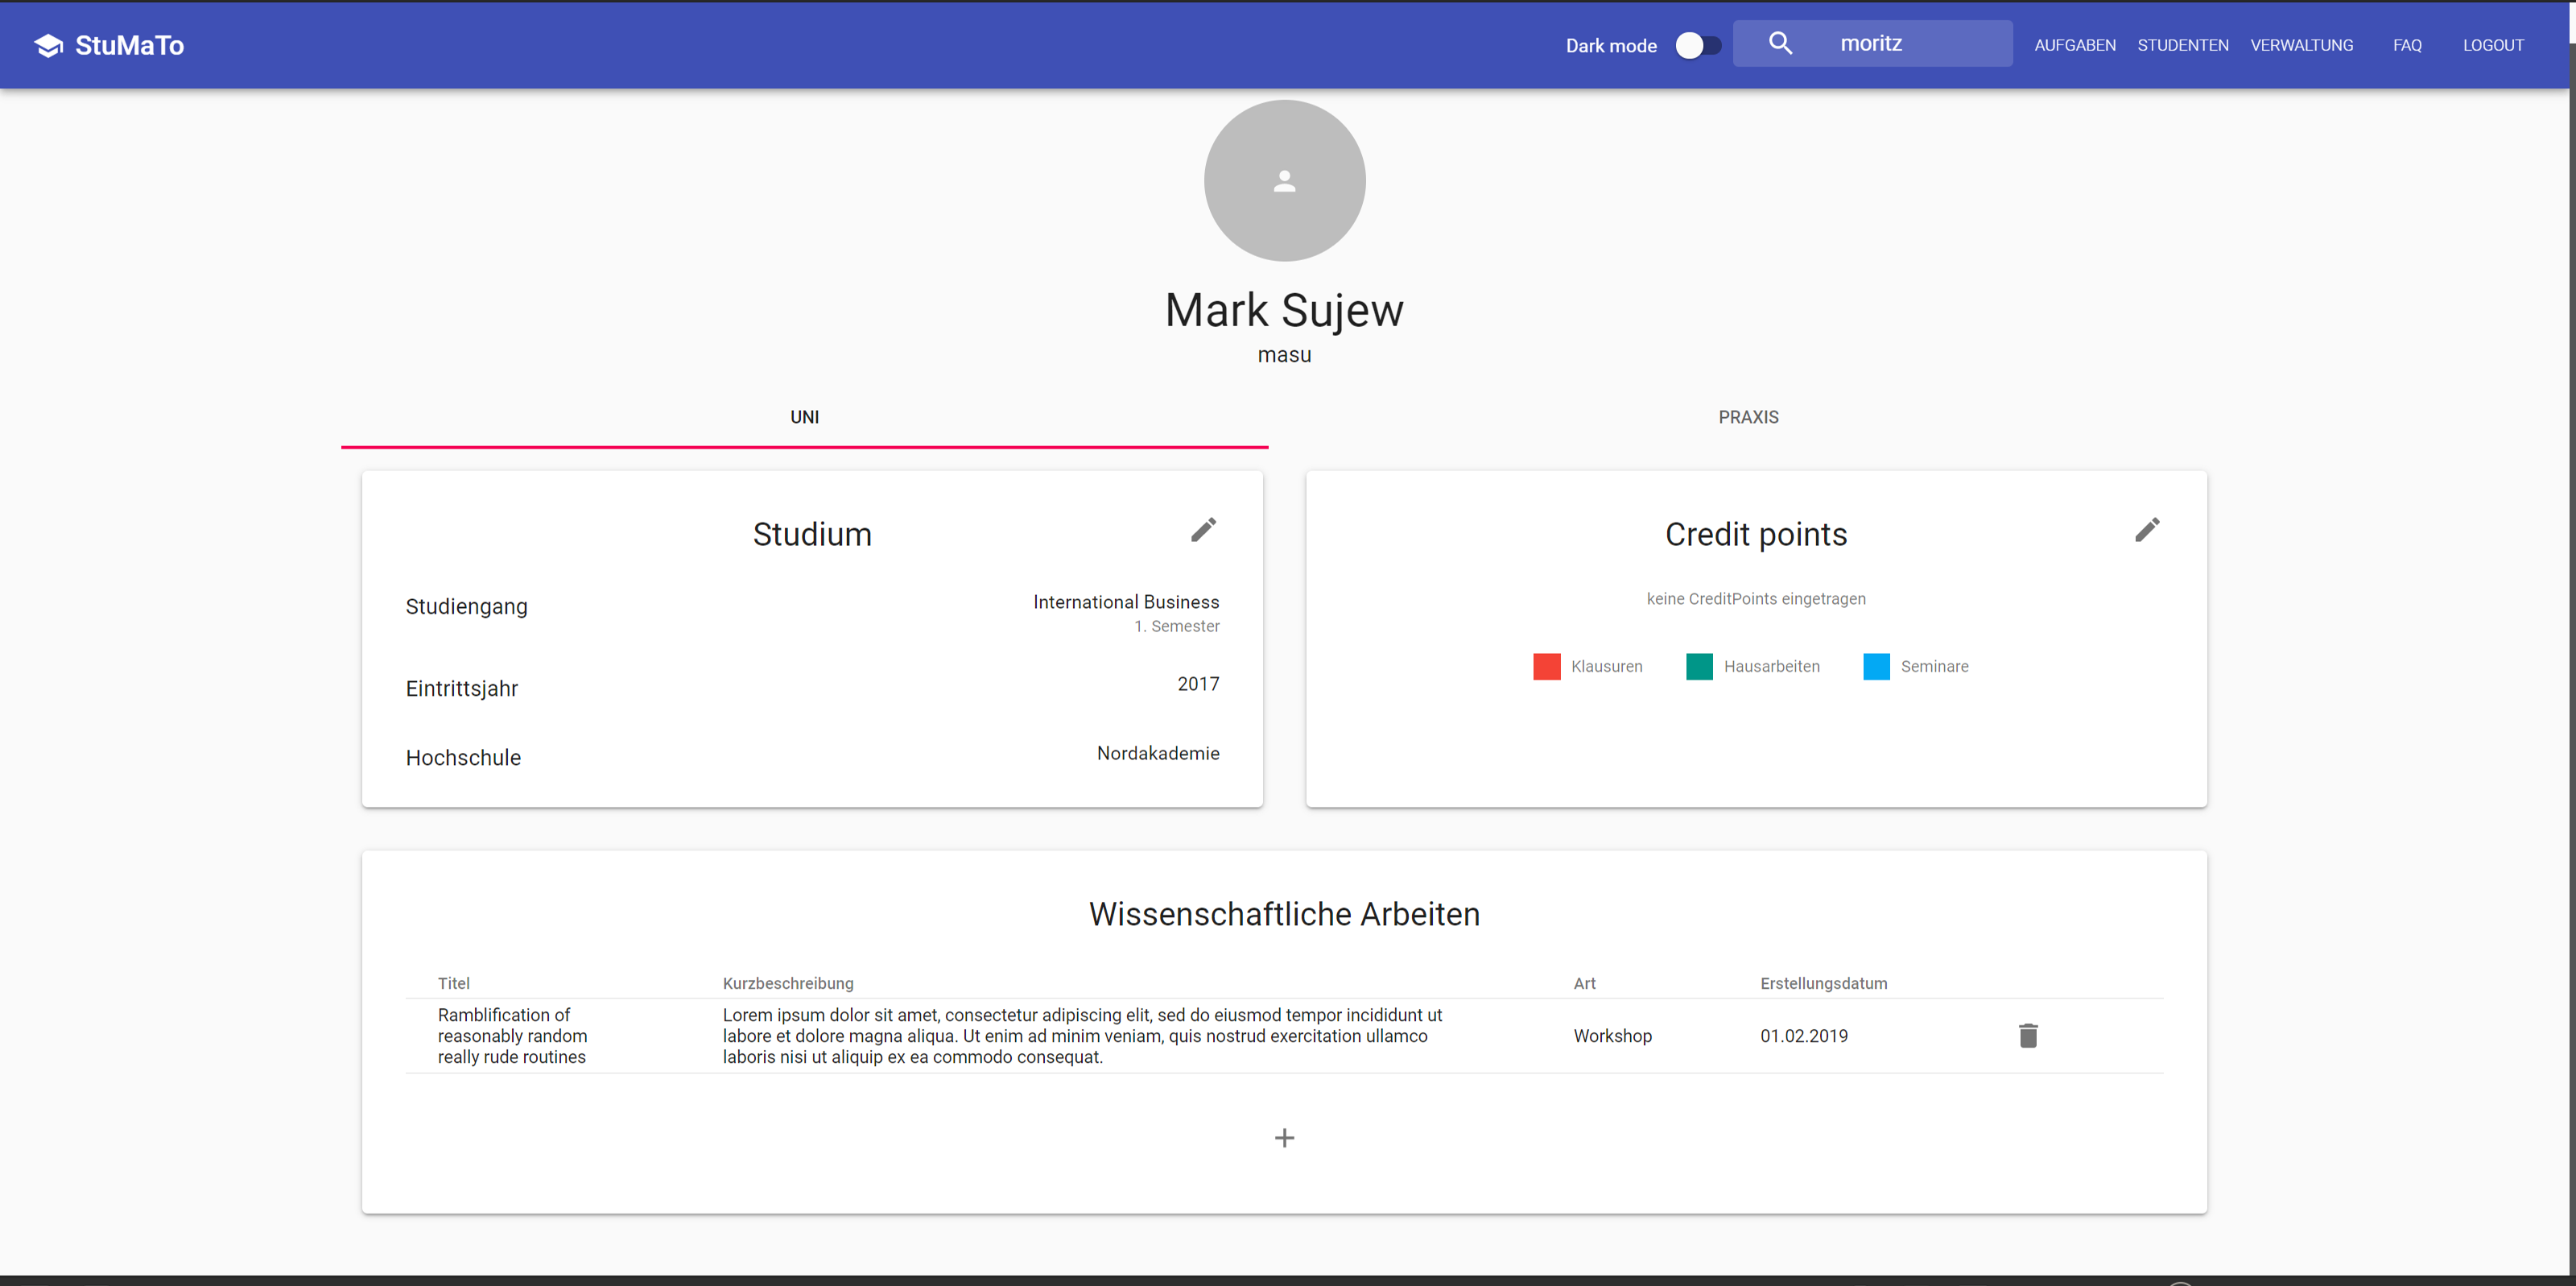
\includegraphics{./tex2pdf.-c803d322dfea80aa/7b7decc77183e1f8259e6c4265ee1b64e115eb3a.png}
\caption{Ansicht STUDENT.UNI}
\end{figure}

\begin{figure}
\centering
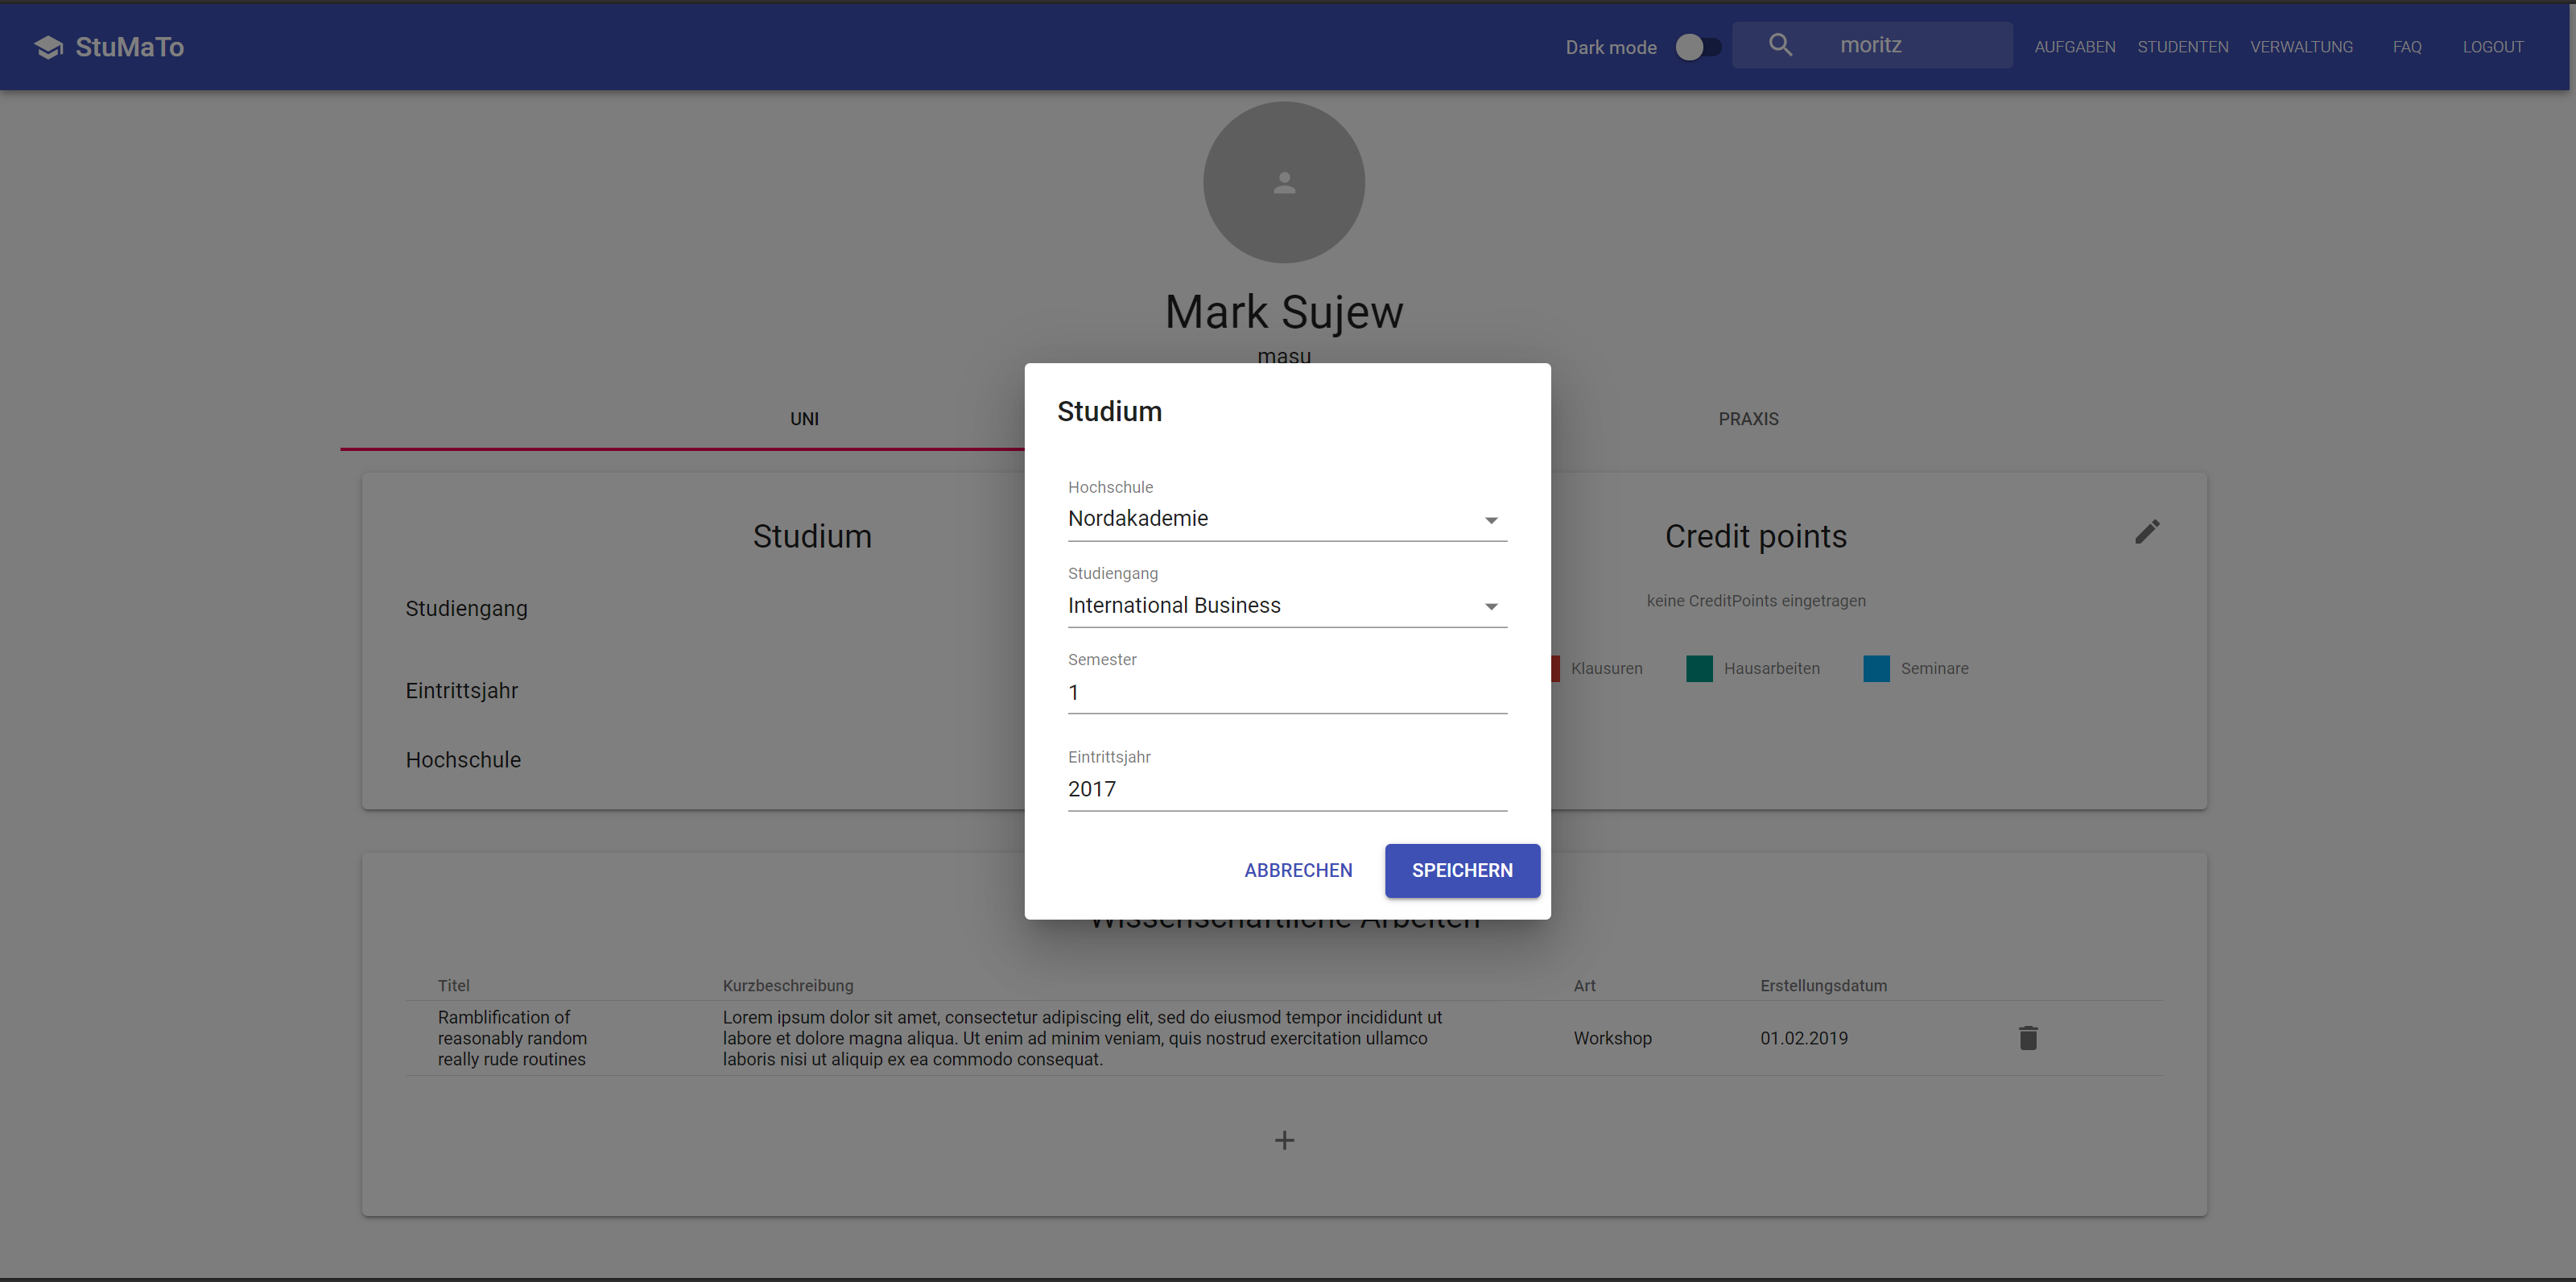
\includegraphics{./tex2pdf.-c803d322dfea80aa/592db6fdc0133bda72392ec386b61b235cfd34b2.png}
\caption{Ansicht STUDENT.UNI.EDIT-STUDY}
\end{figure}

\begin{figure}
\centering
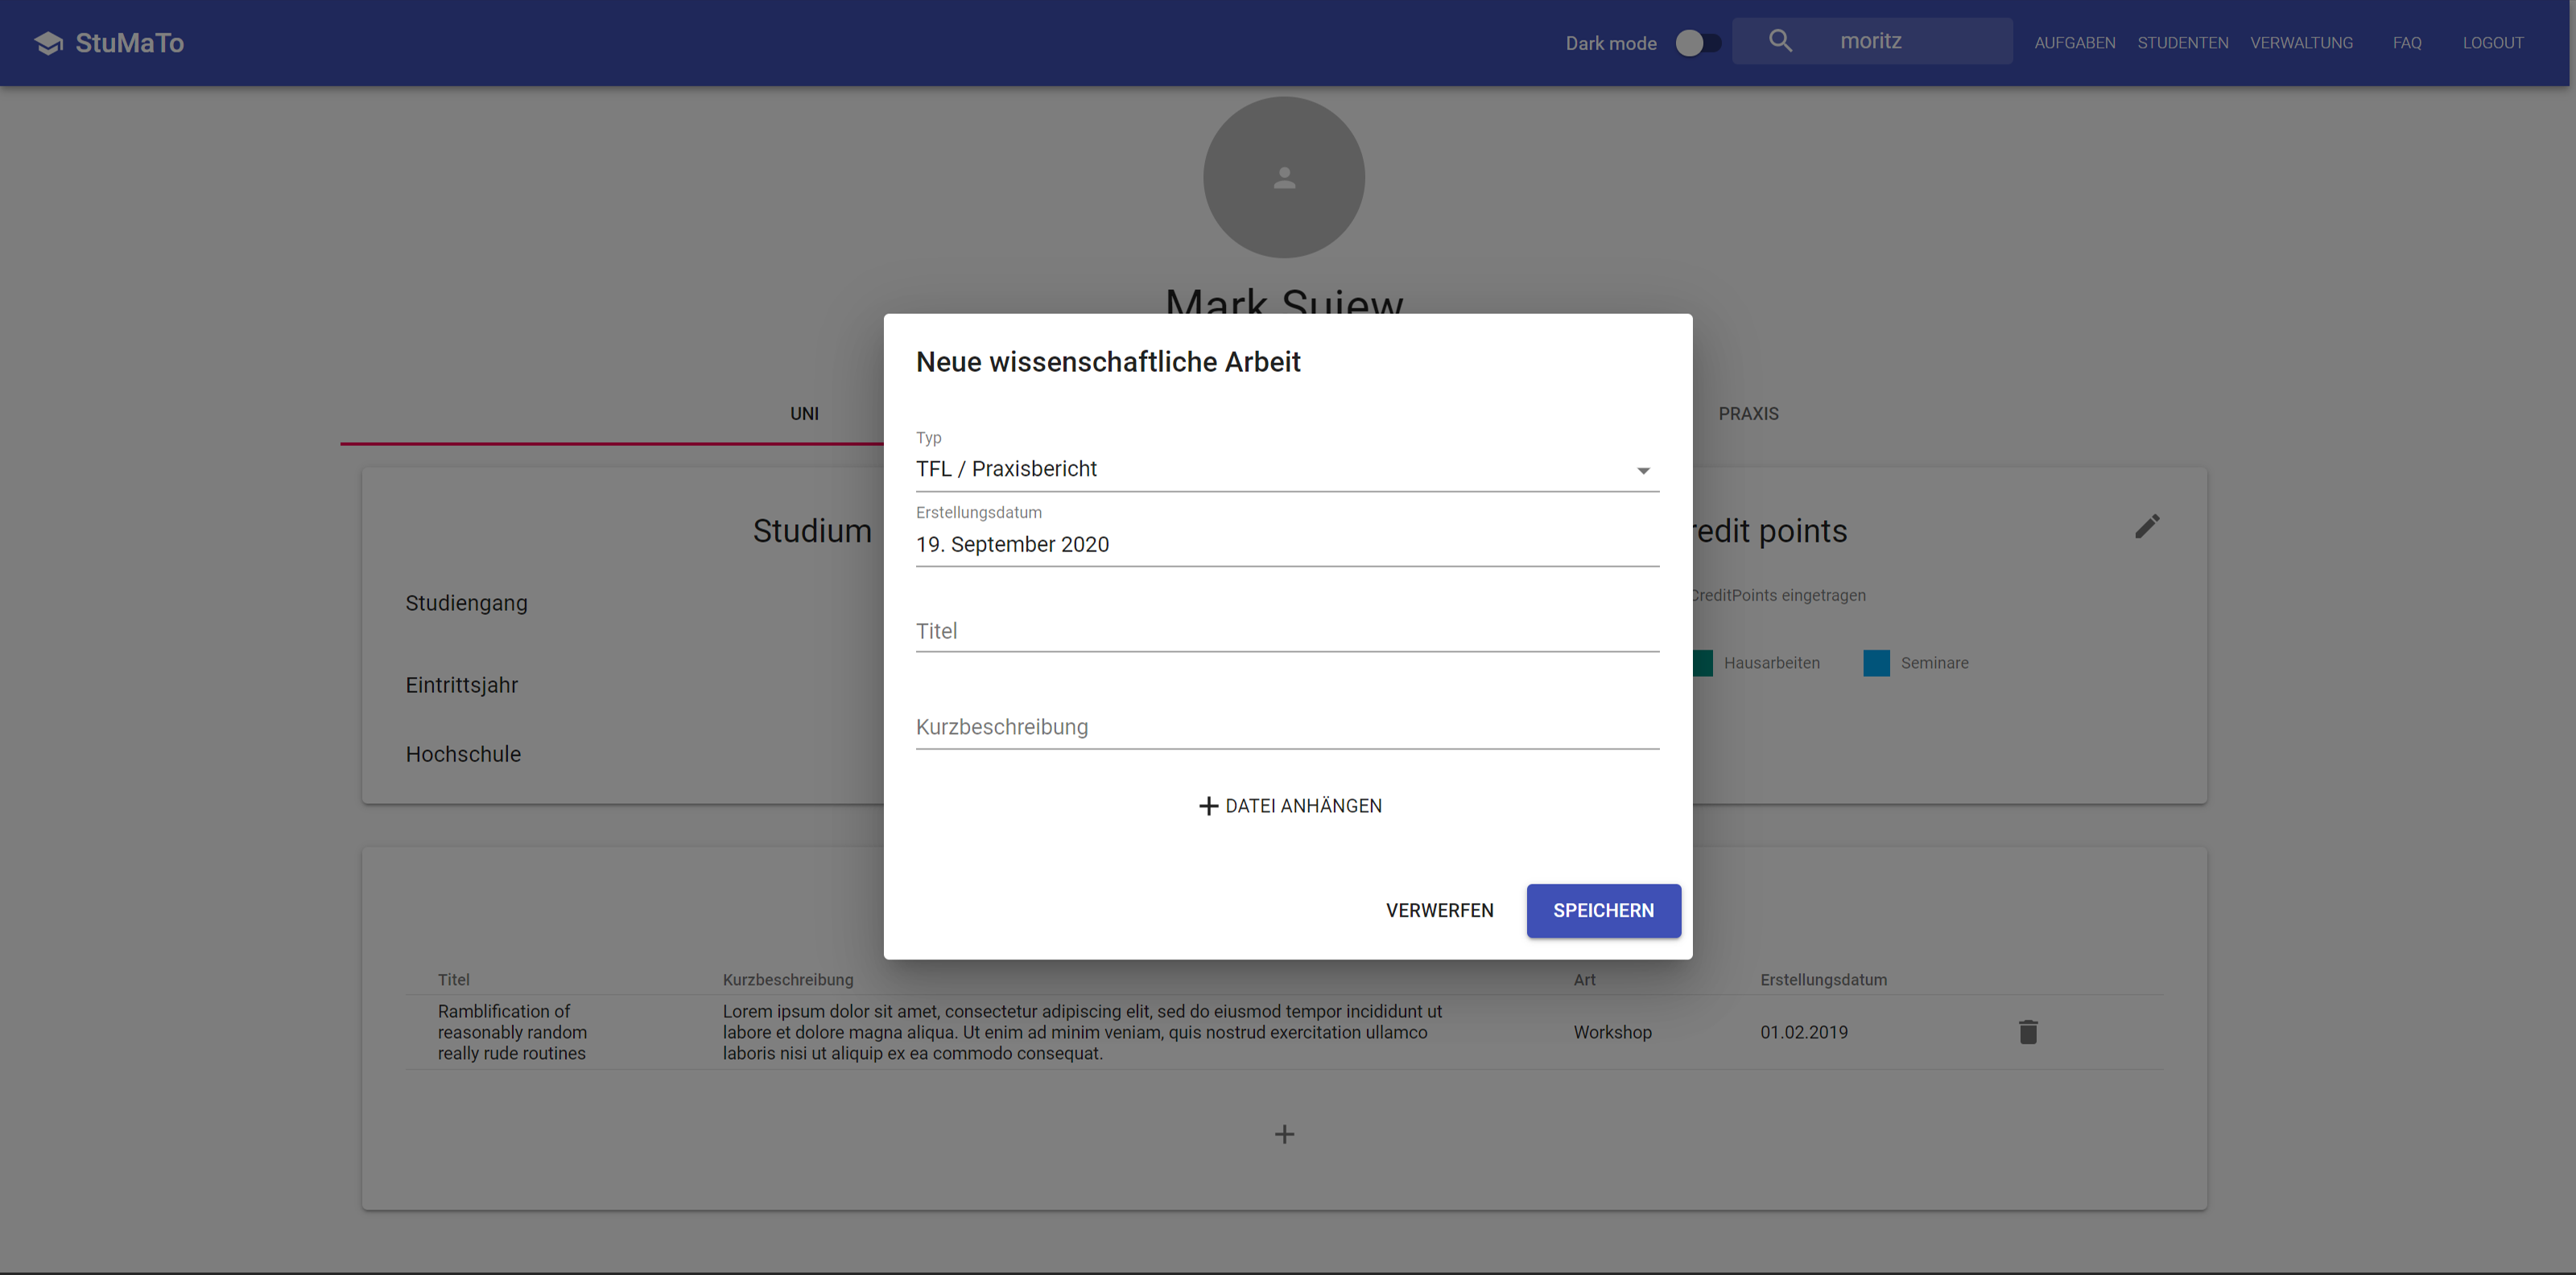
\includegraphics{./tex2pdf.-c803d322dfea80aa/c8129831c98a80007f8fd71f31b9f91dda318a5d.png}
\caption{Ansicht STUDENT.UNI.NEW-TFL}
\end{figure}

\begin{figure}
\centering
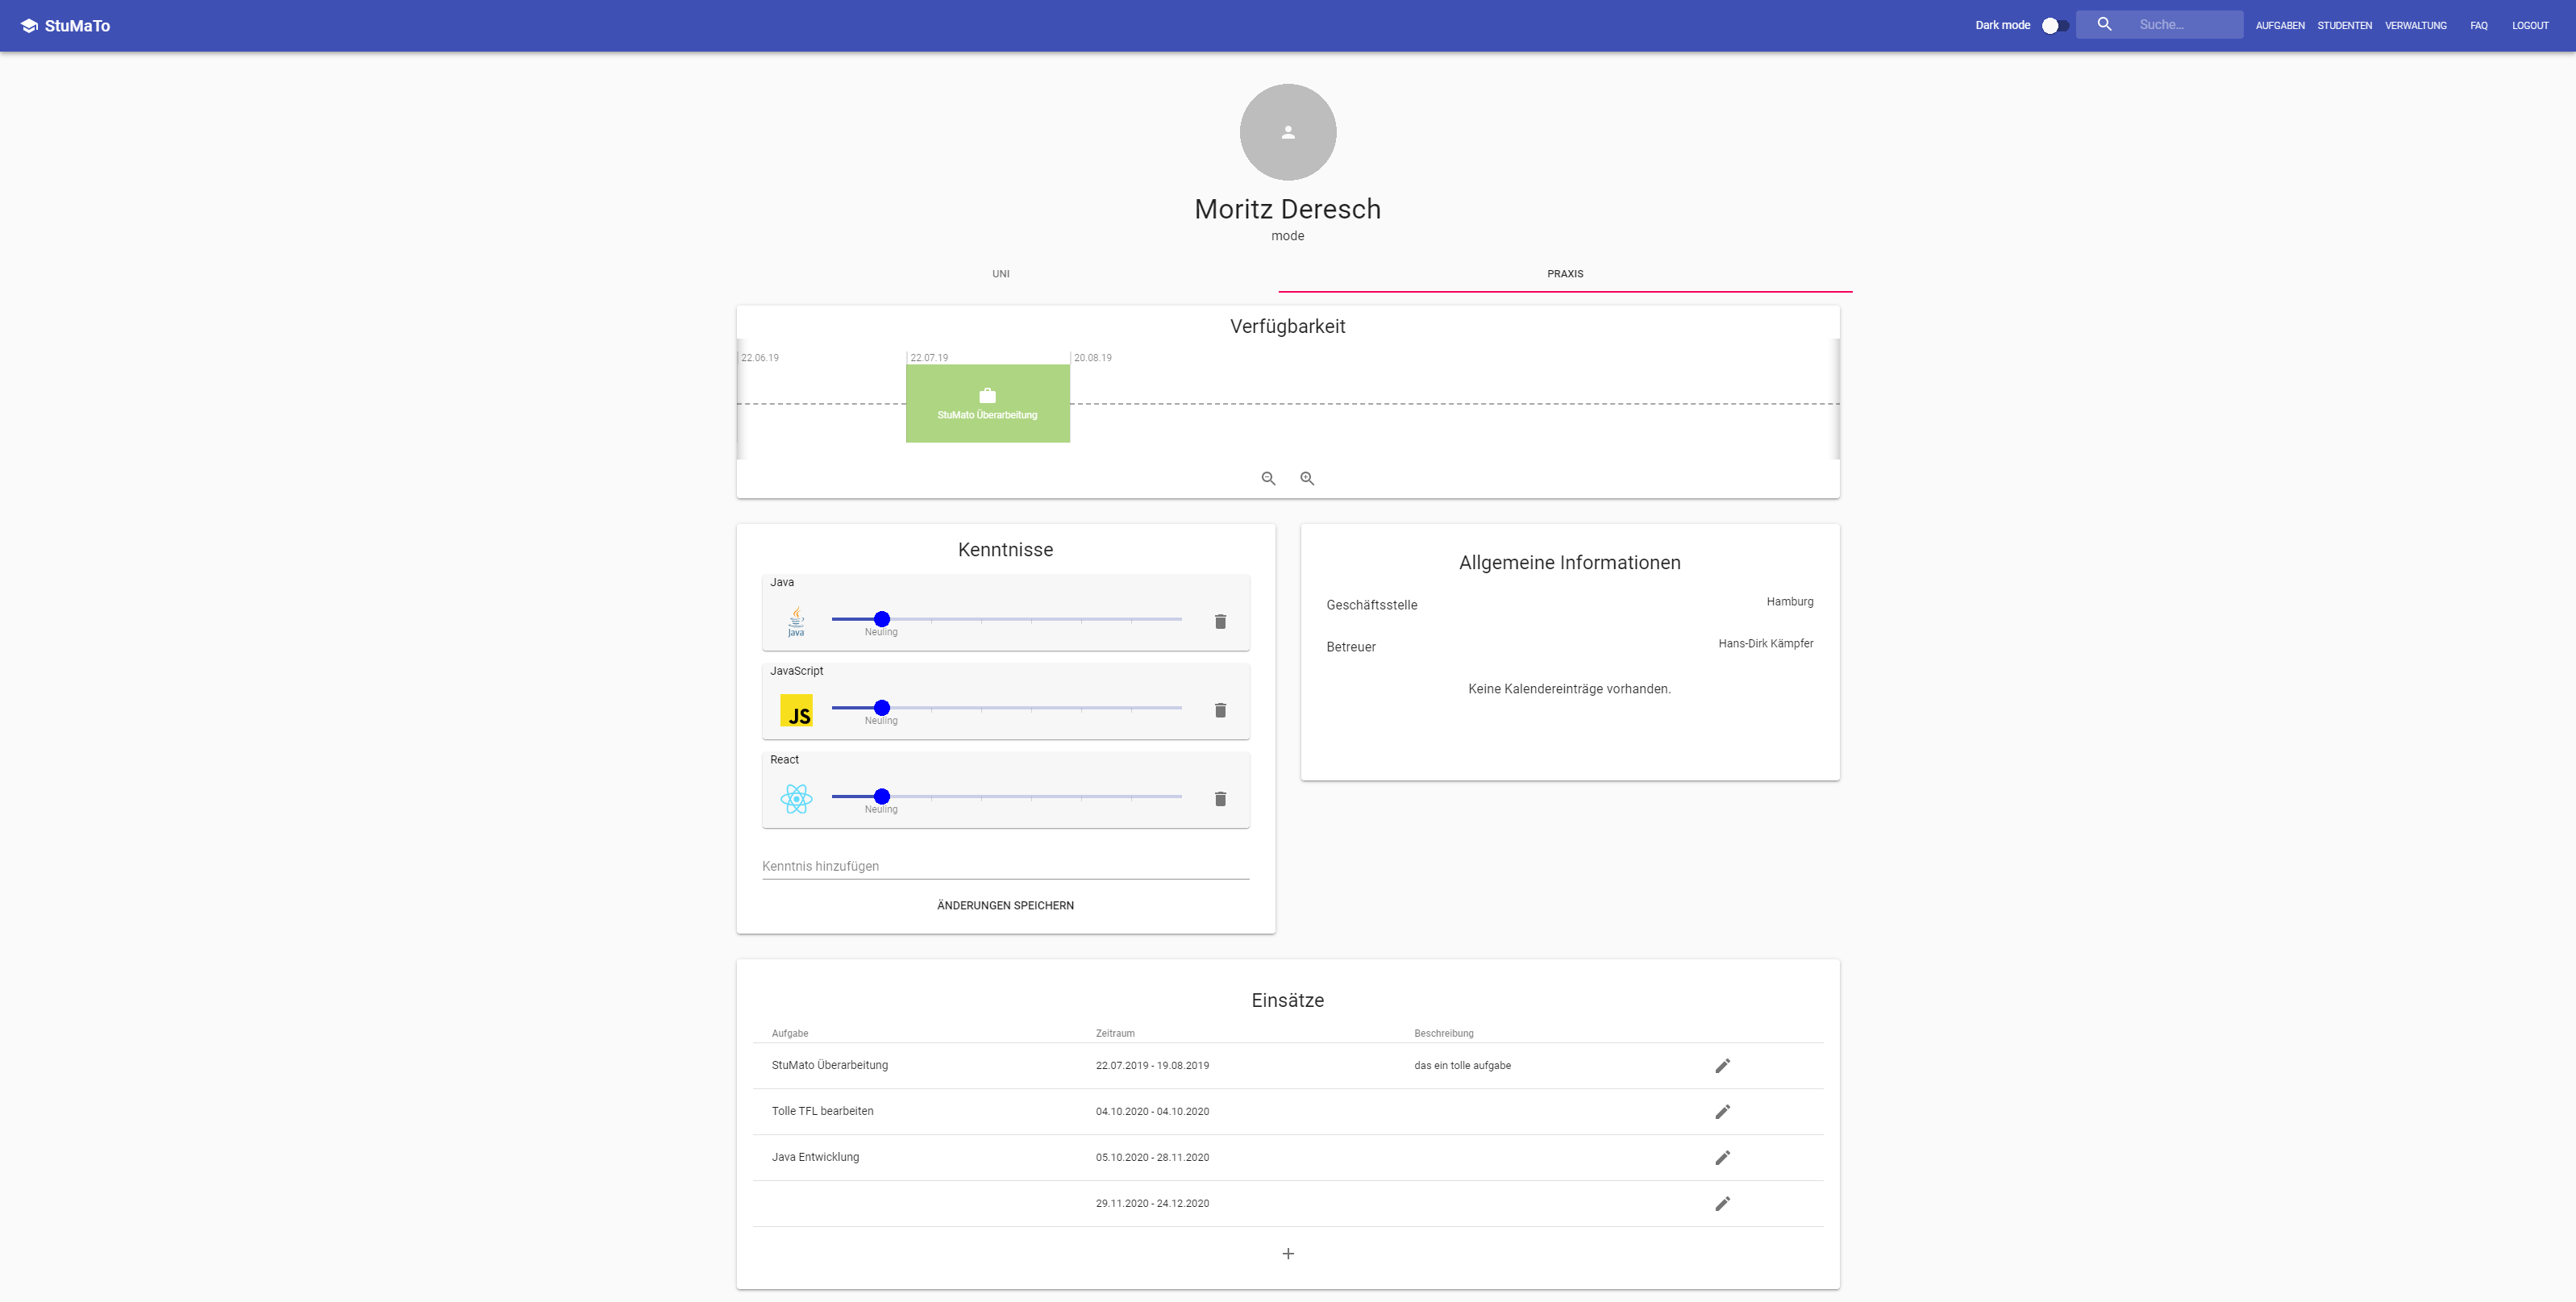
\includegraphics{./tex2pdf.-c803d322dfea80aa/3fcf93b7c7c70c0ec7ba98351dd035514a9bc92b.png}
\caption{Ansicht STUDENT.WORK}
\end{figure}

\begin{figure}
\centering
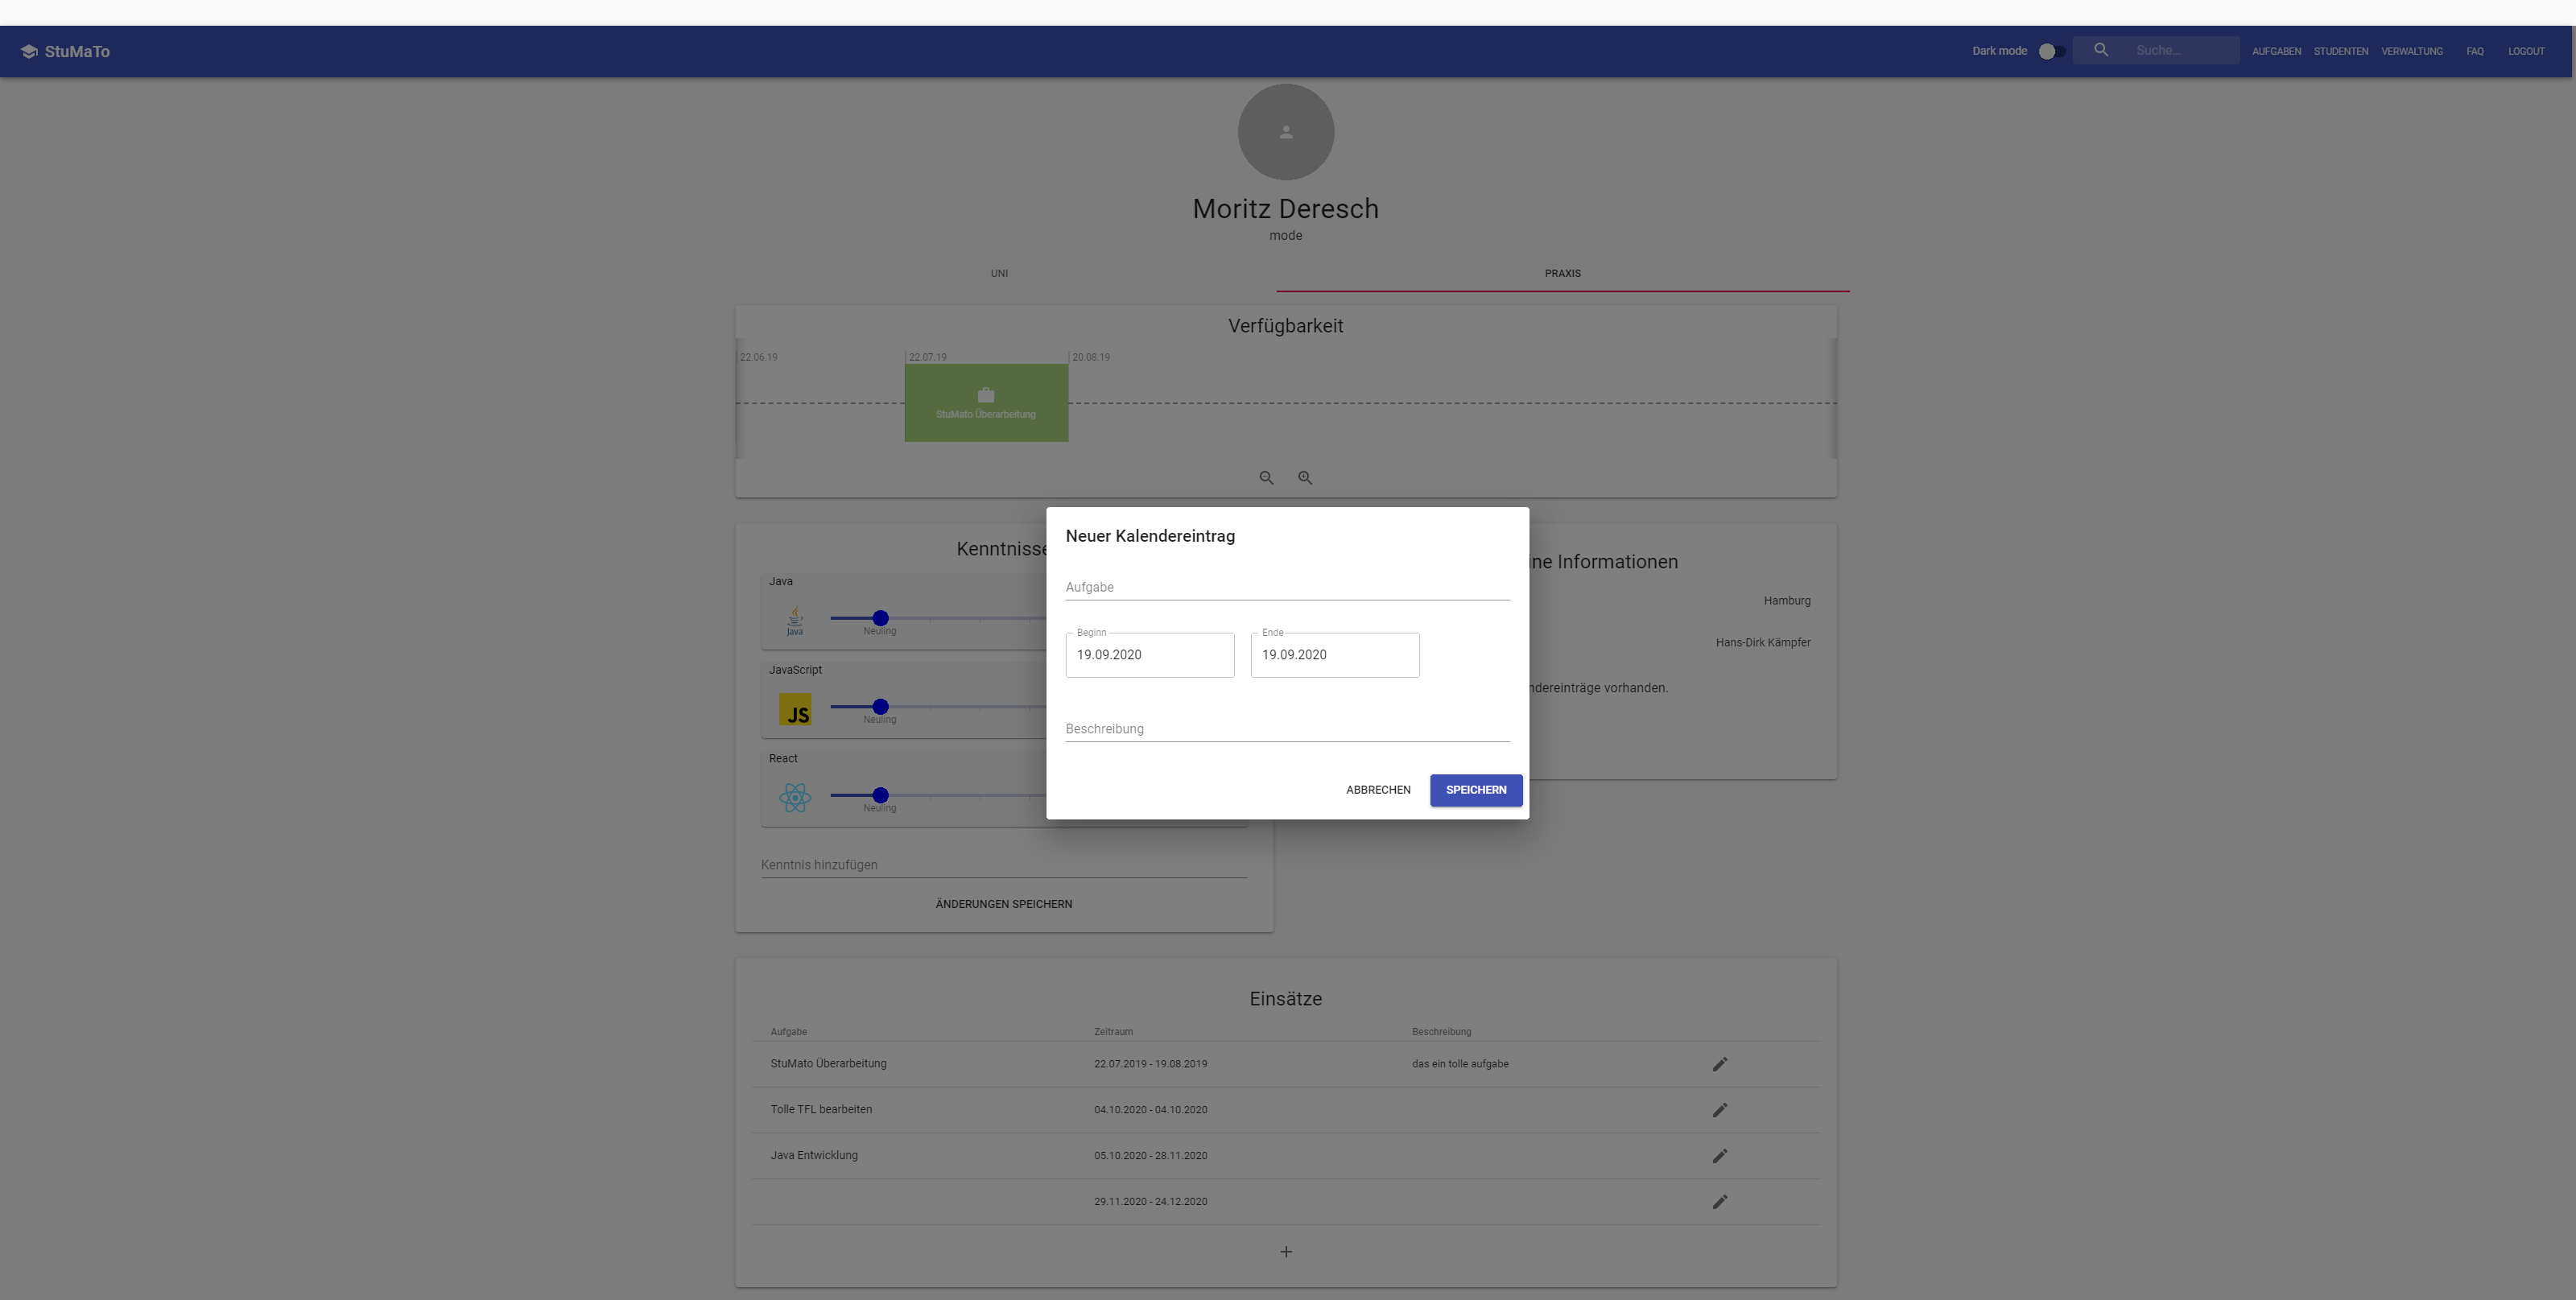
\includegraphics{./tex2pdf.-c803d322dfea80aa/e861a0f50de01e967b15da07f60cce10b9c4e729.png}
\caption{Ansicht STUDENT.WORK.NEW-ENTRY}
\end{figure}

\begin{figure}
\centering
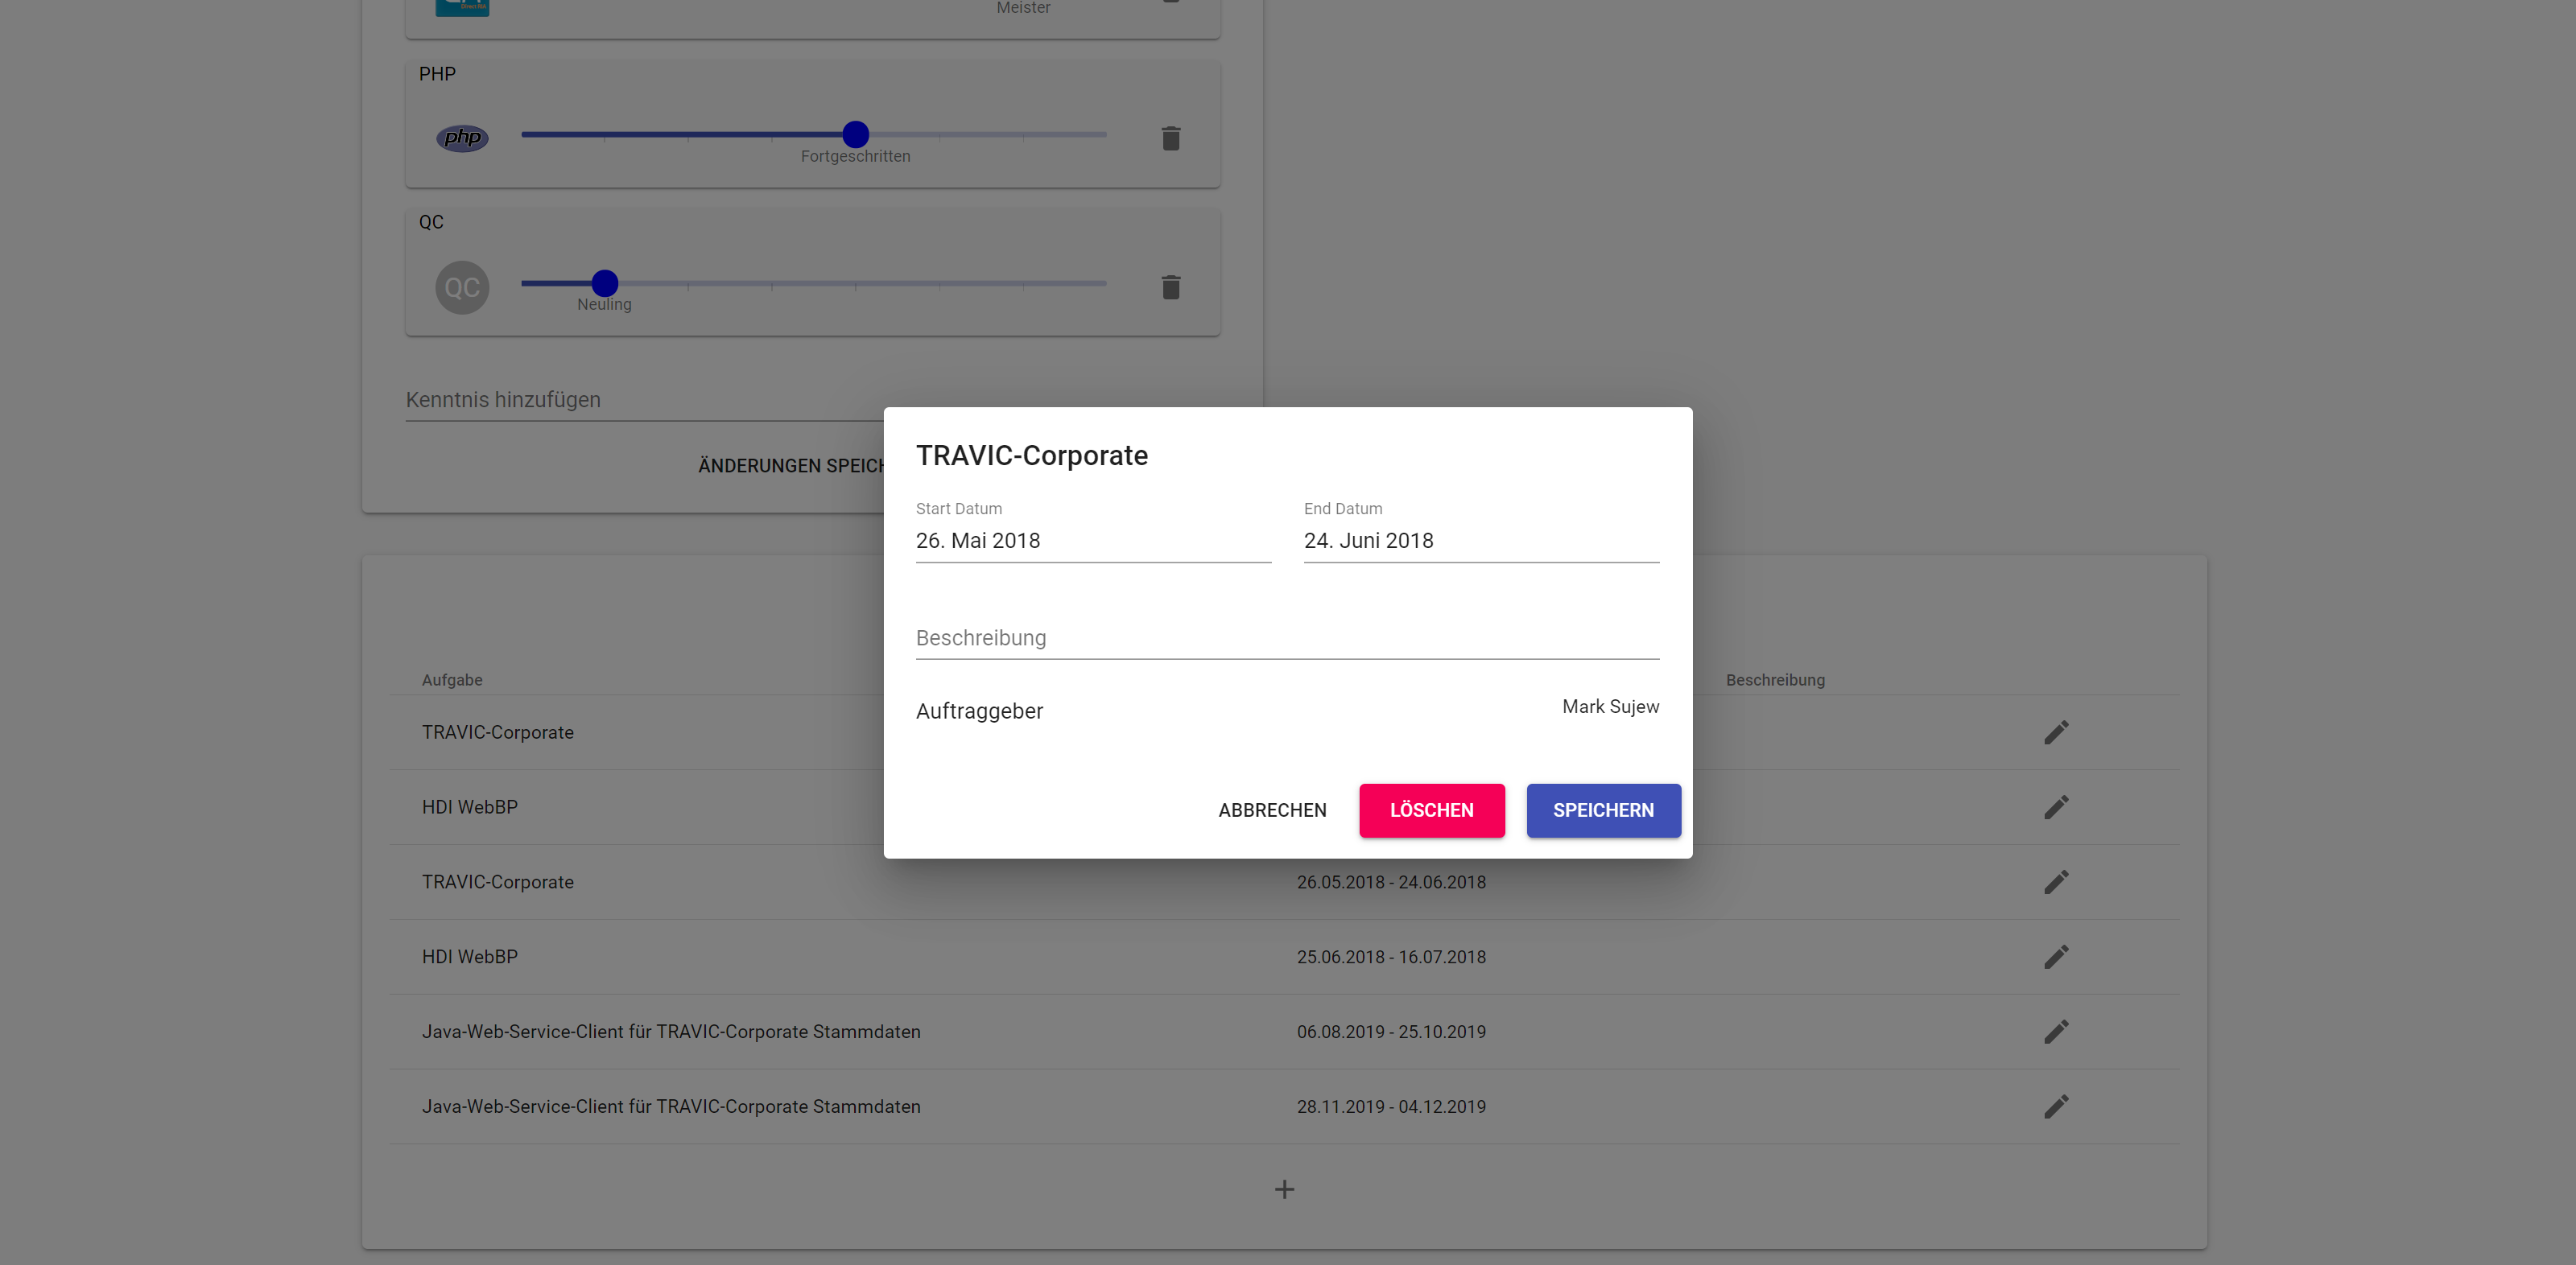
\includegraphics{./tex2pdf.-c803d322dfea80aa/4c63a93237317c668e20509da7541b02094f7800.png}
\caption{Ansicht STUDENT.WORK.EDIT-ENTRY}
\end{figure}

\begin{figure}
\centering
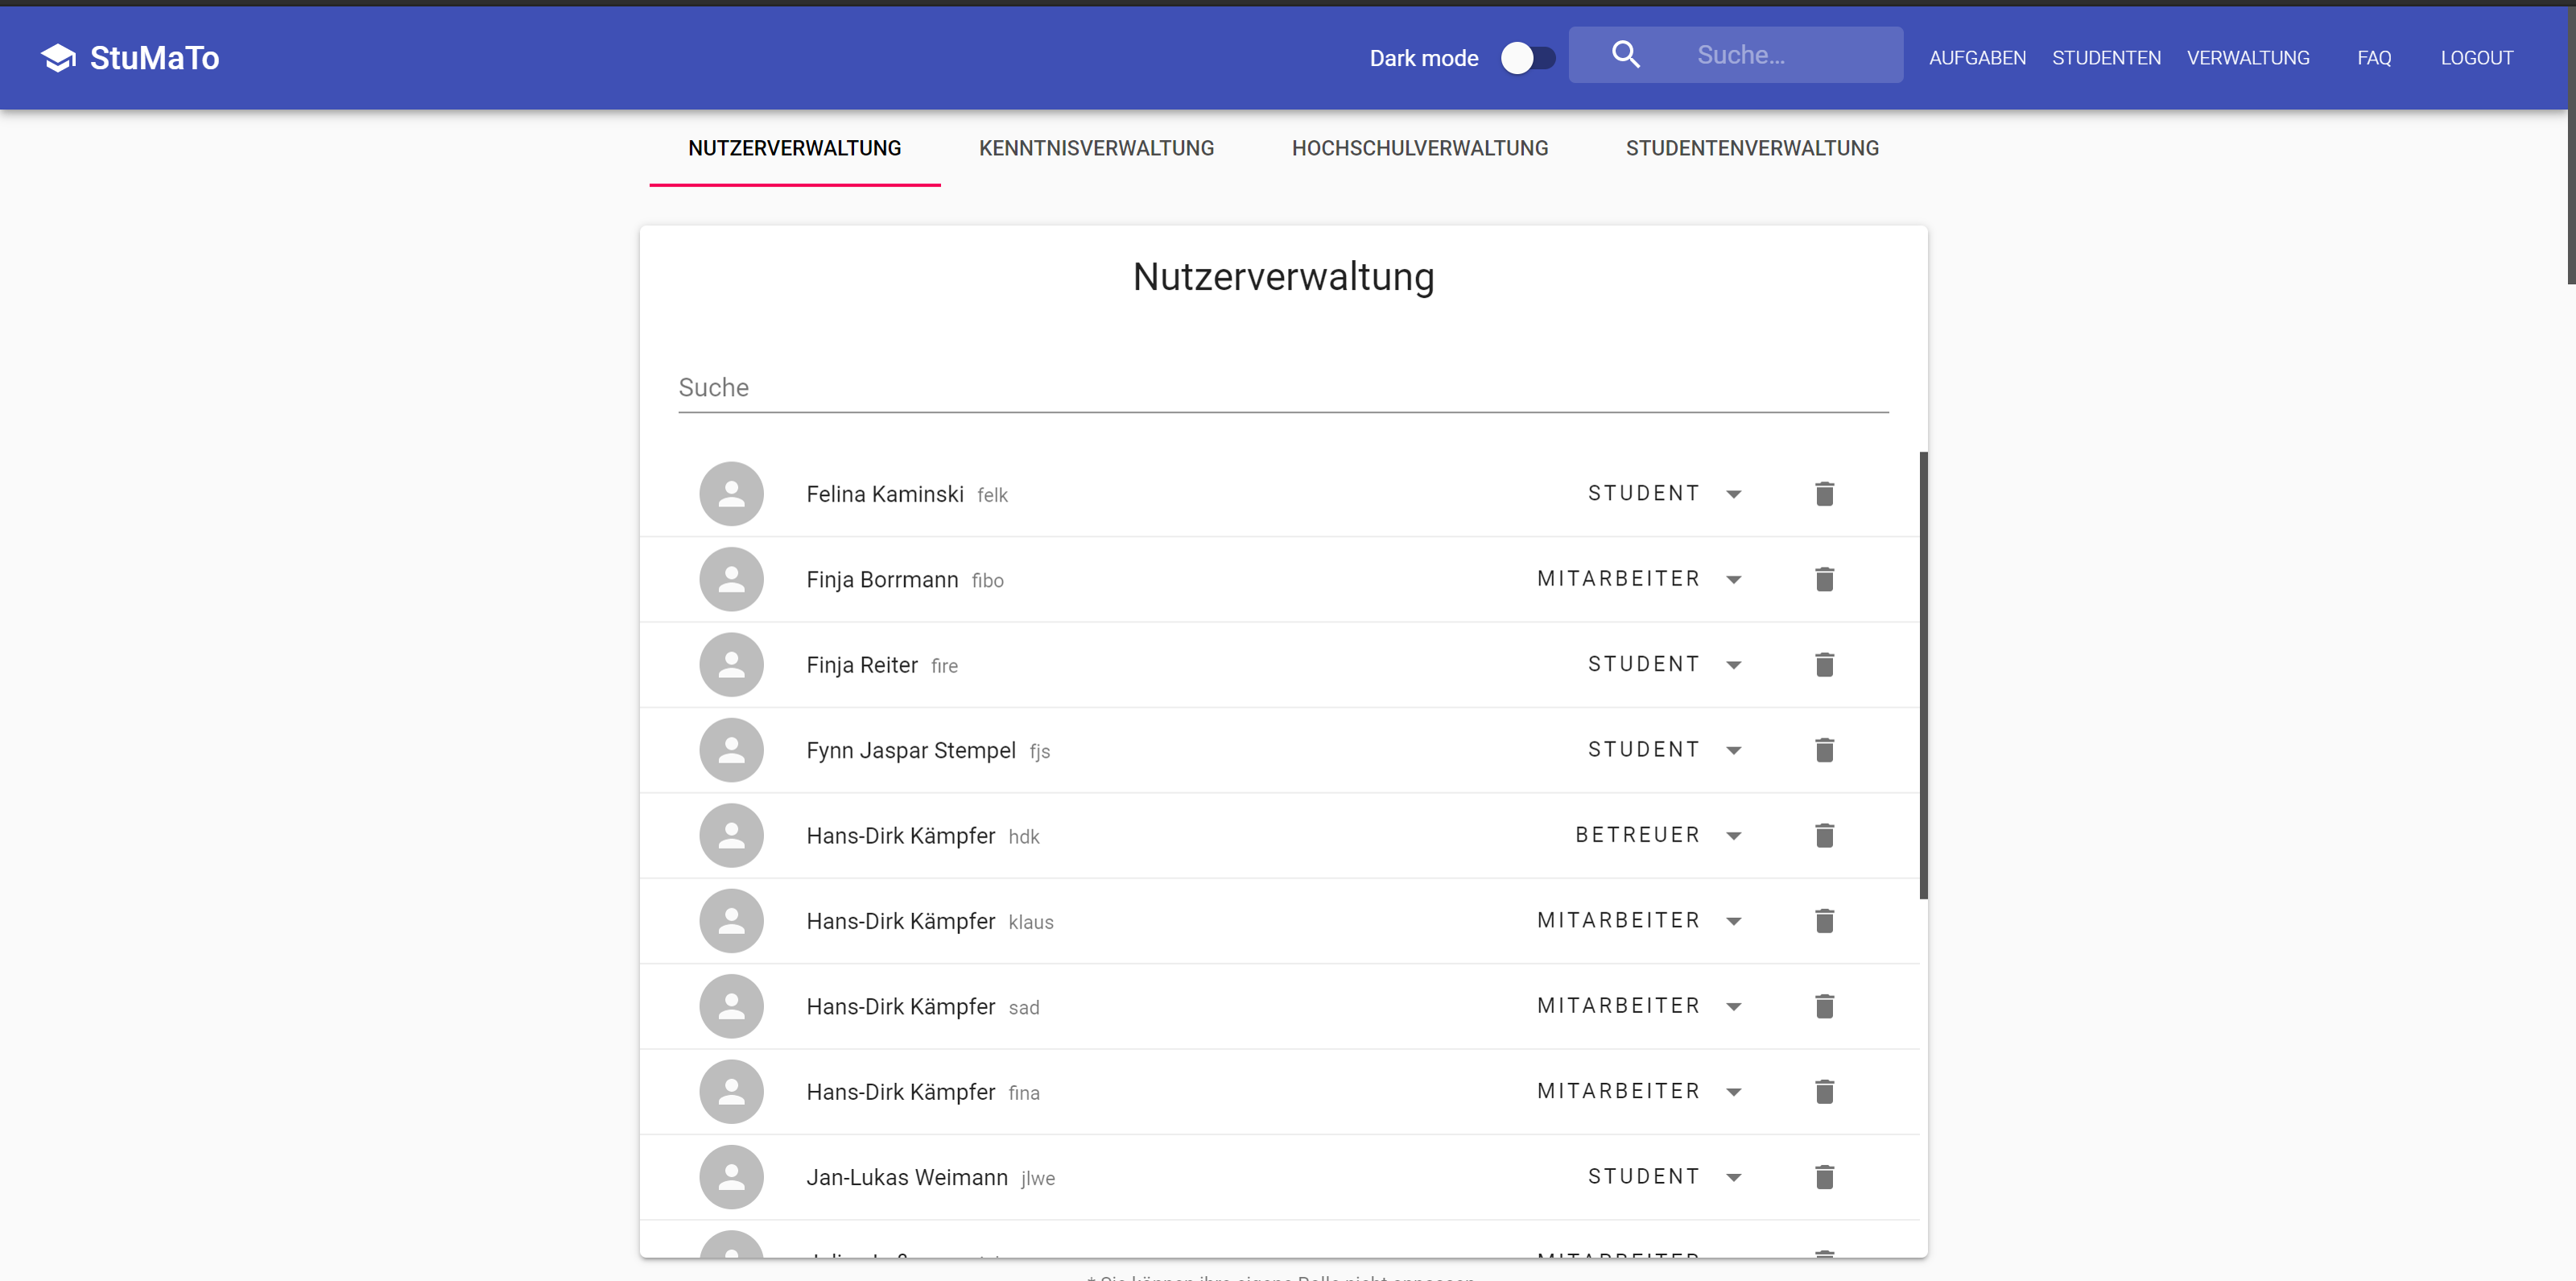
\includegraphics{./tex2pdf.-c803d322dfea80aa/a755eb96a92ad6d15e845ce1cce757327b2d571b.png}
\caption{Ansicht MANAGE.USER}
\end{figure}

\begin{figure}
\centering
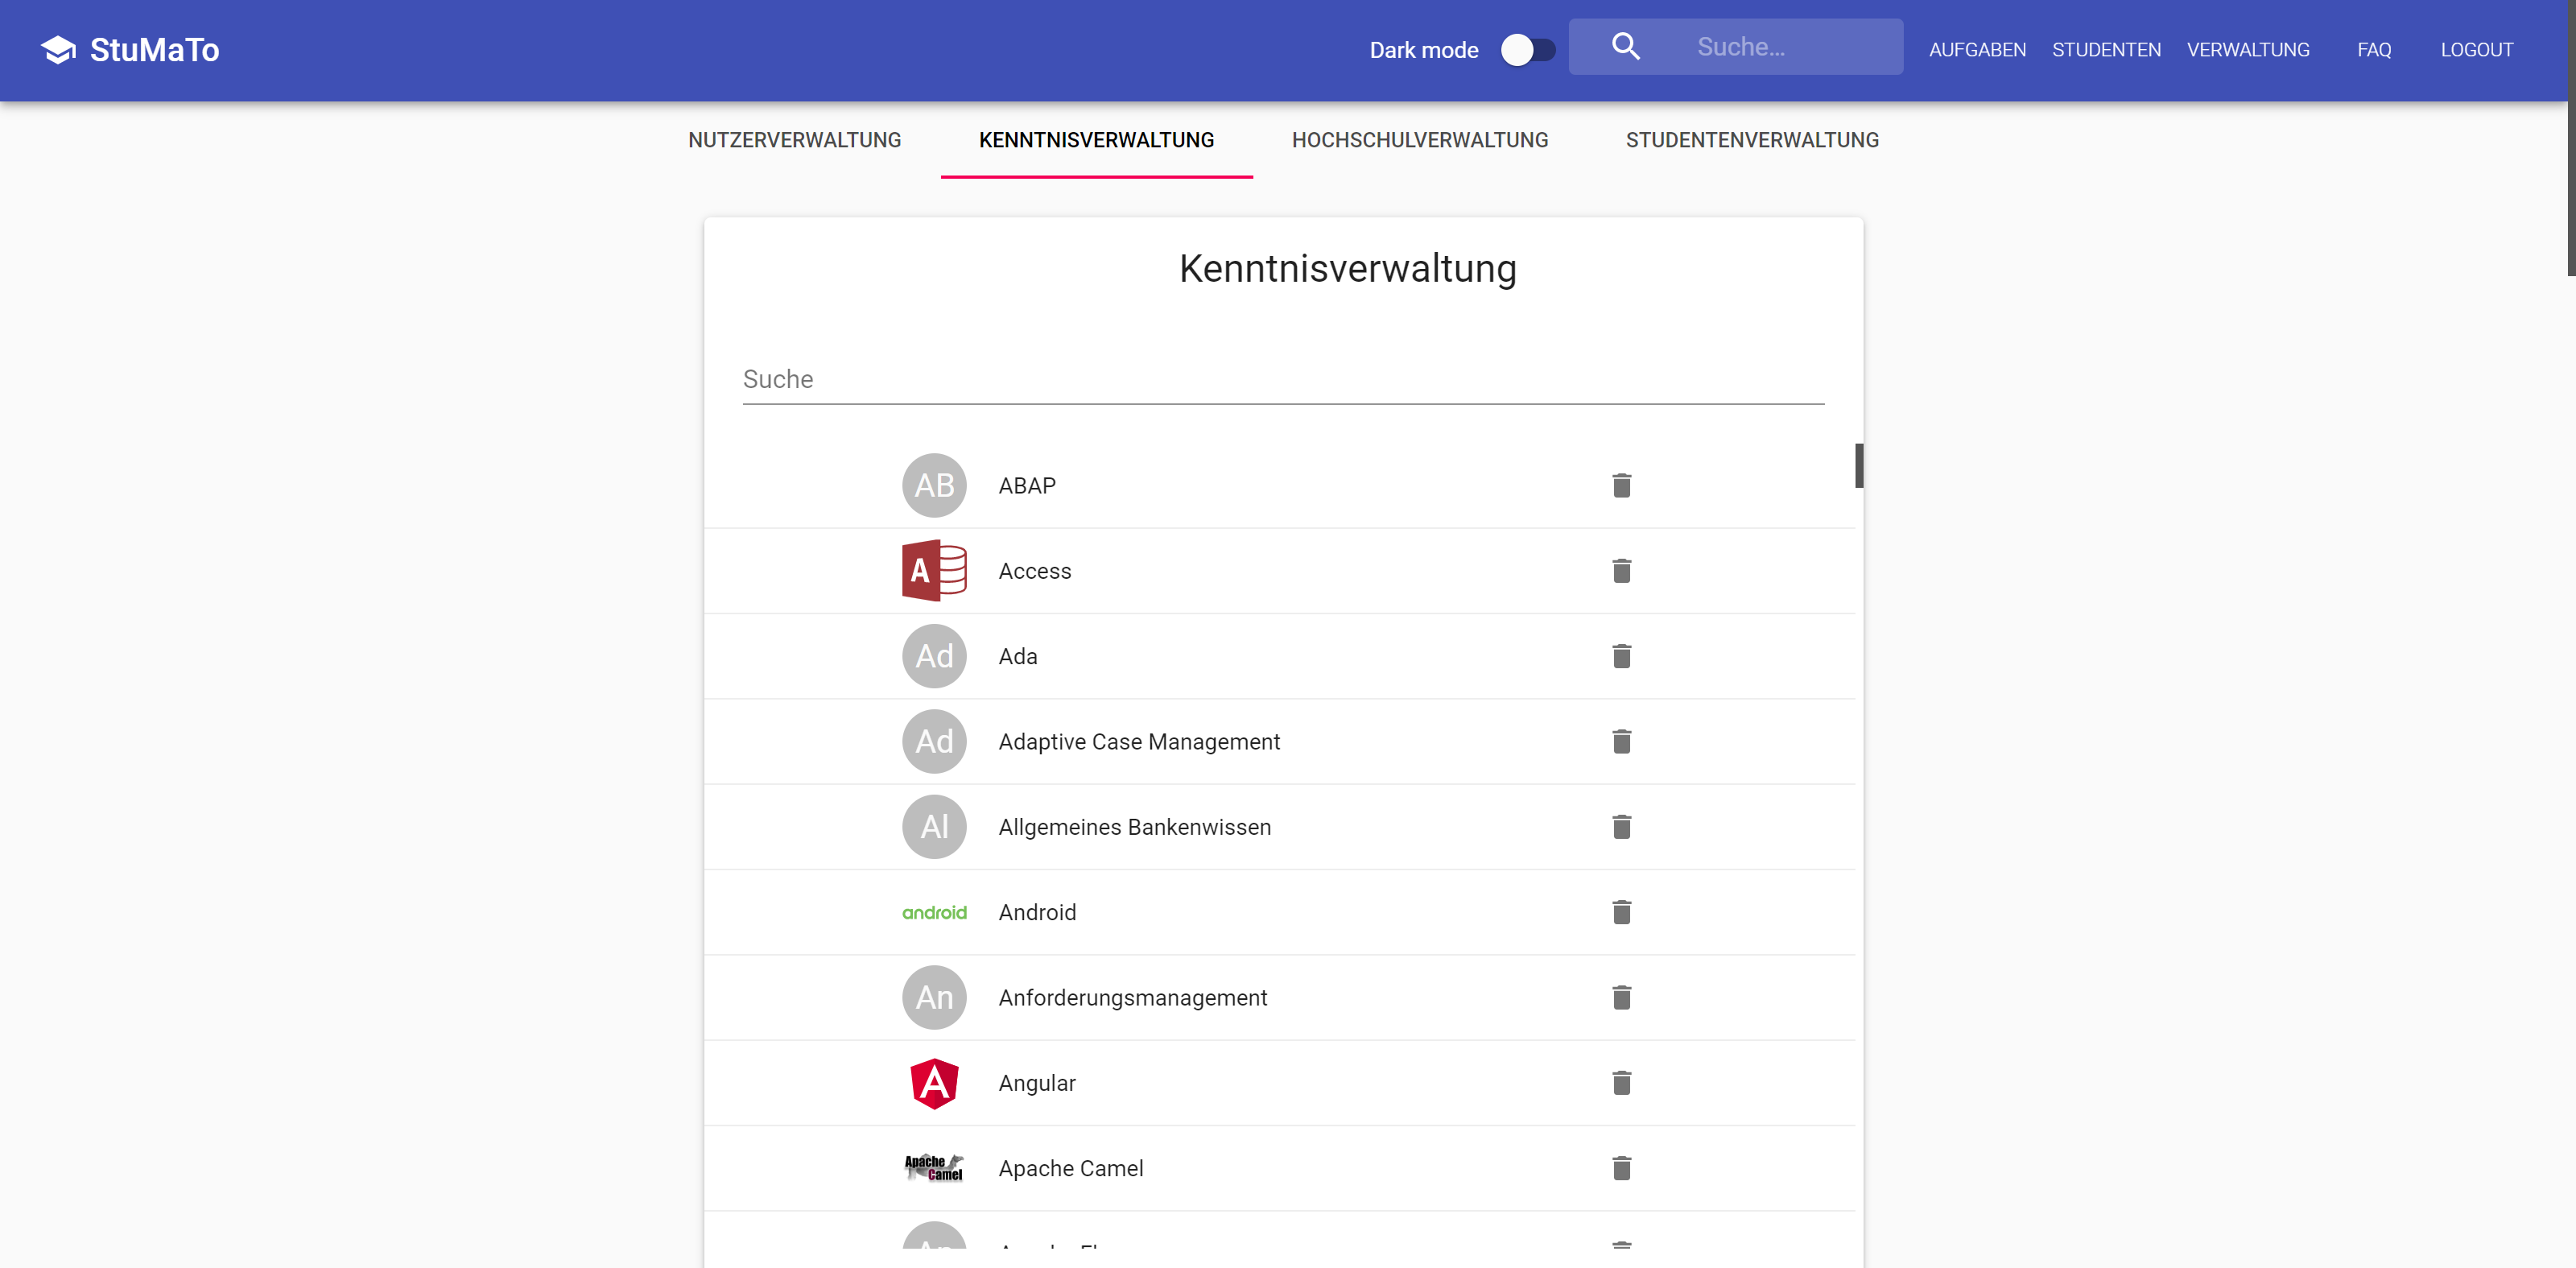
\includegraphics{./tex2pdf.-c803d322dfea80aa/ce3458428610c575dda494aa3efaffc445fa738a.png}
\caption{Ansicht MANAGE.SKILLS}
\end{figure}

\begin{figure}
\centering
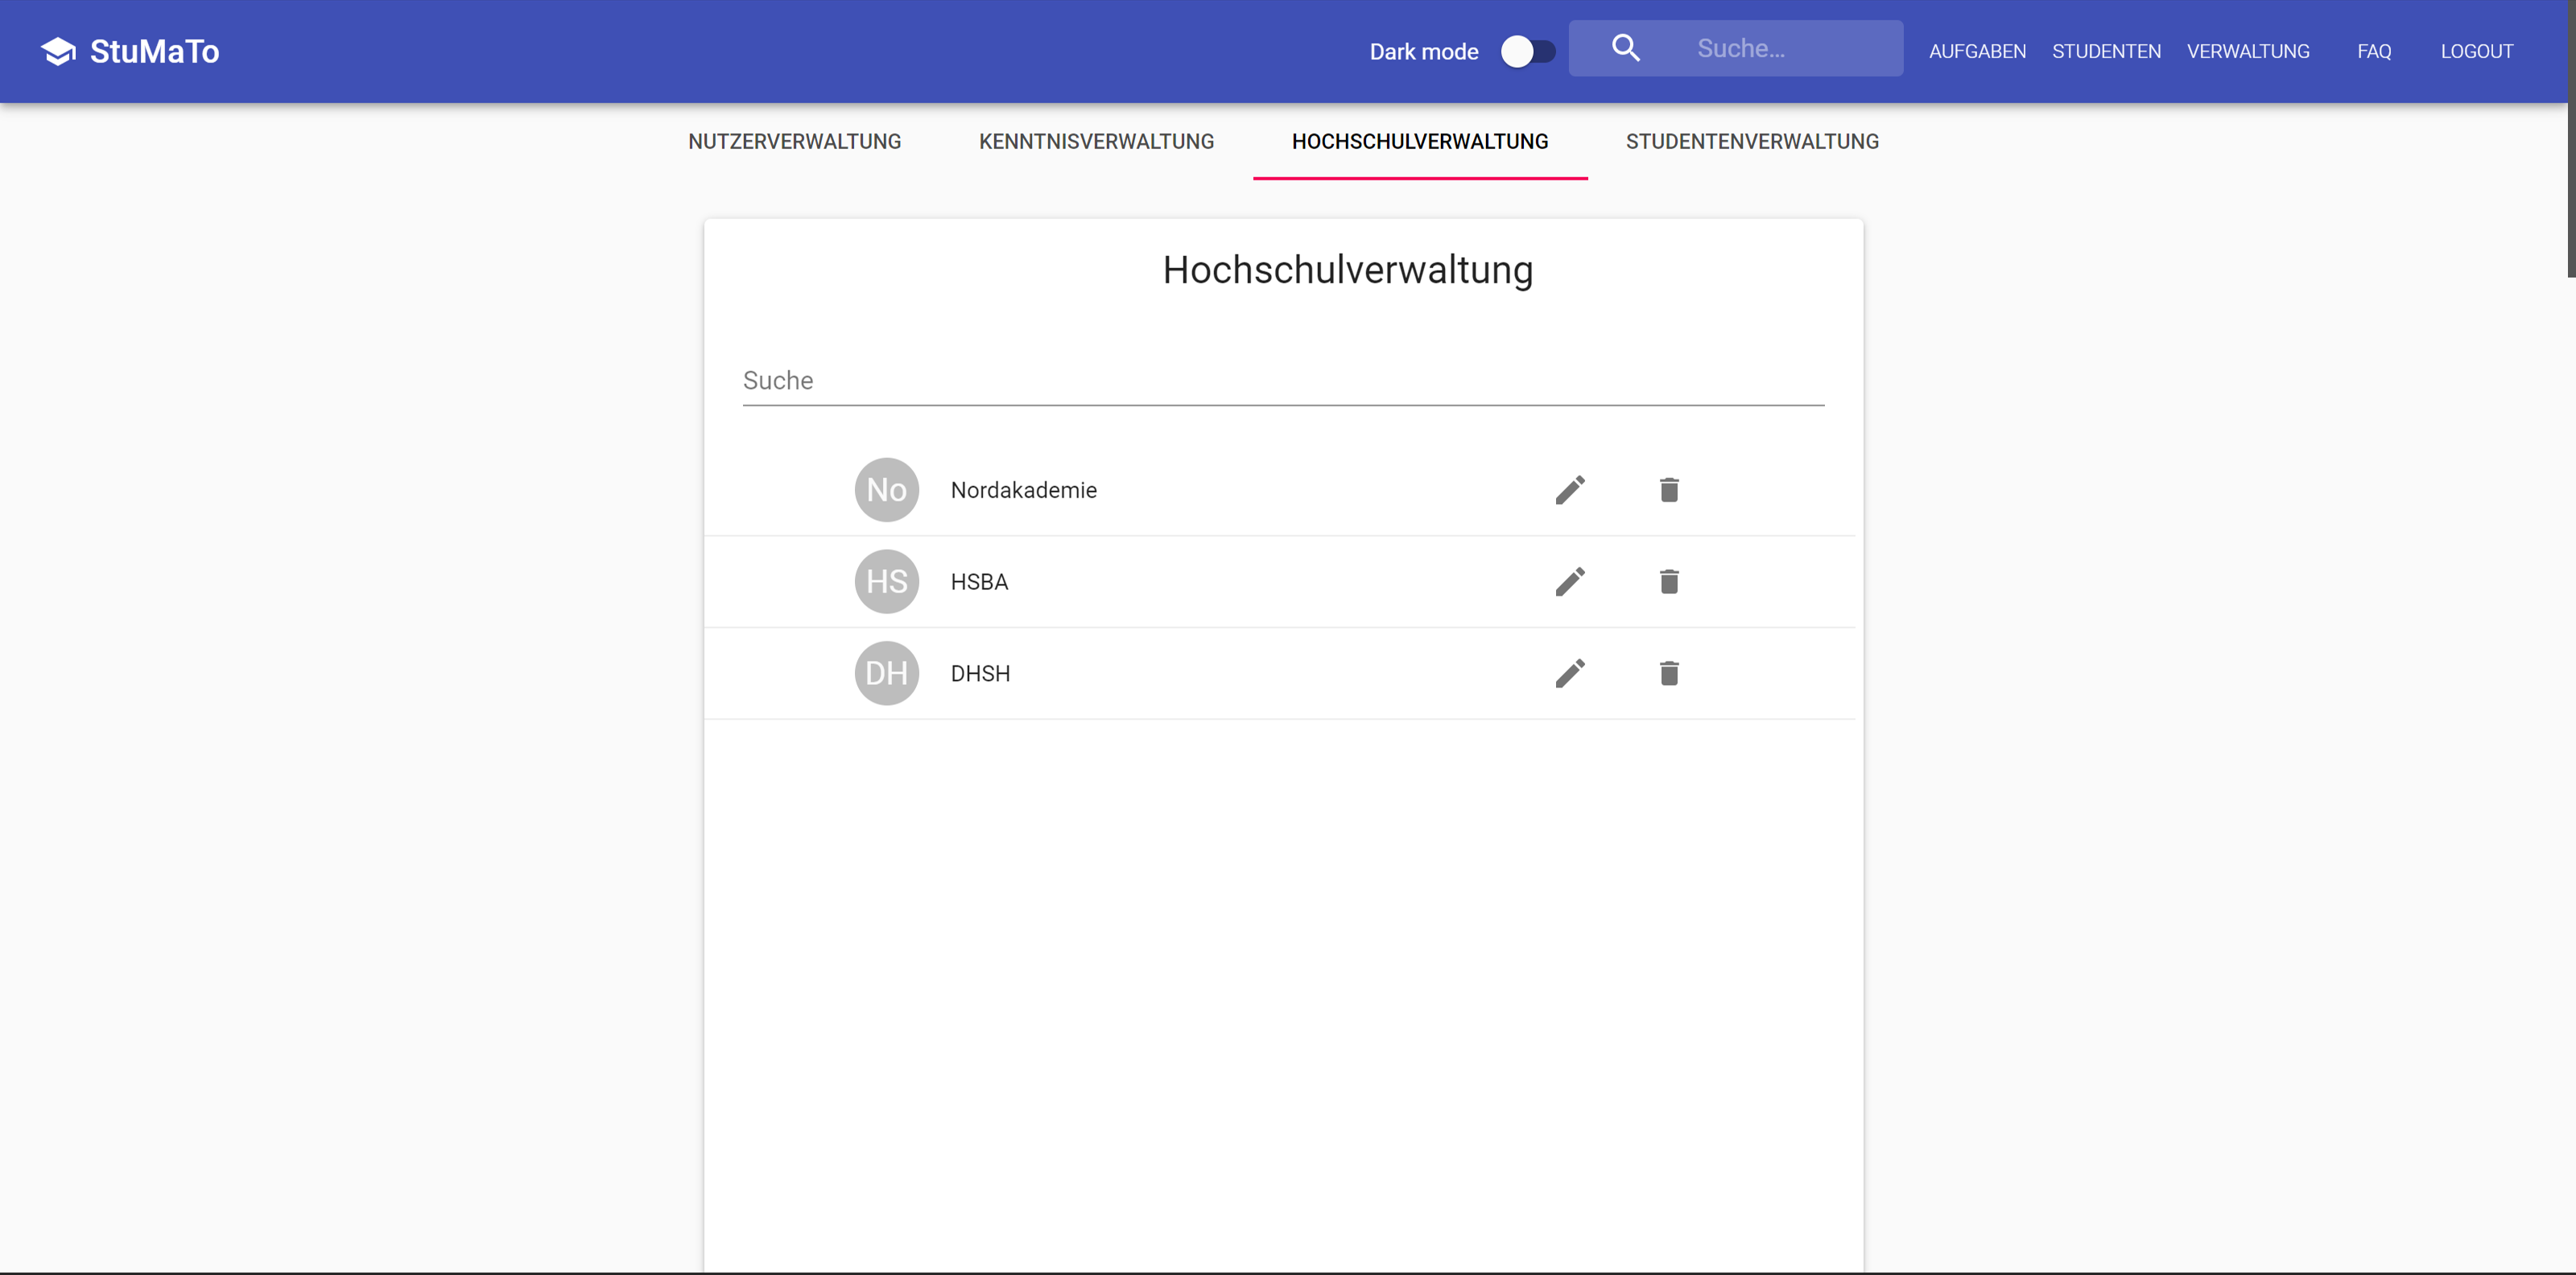
\includegraphics{./tex2pdf.-c803d322dfea80aa/84843a33decc9c7d289ff6cdcdf6eee152dcc7c0.png}
\caption{Ansicht MANAGE.UNI}
\end{figure}

\begin{figure}
\centering
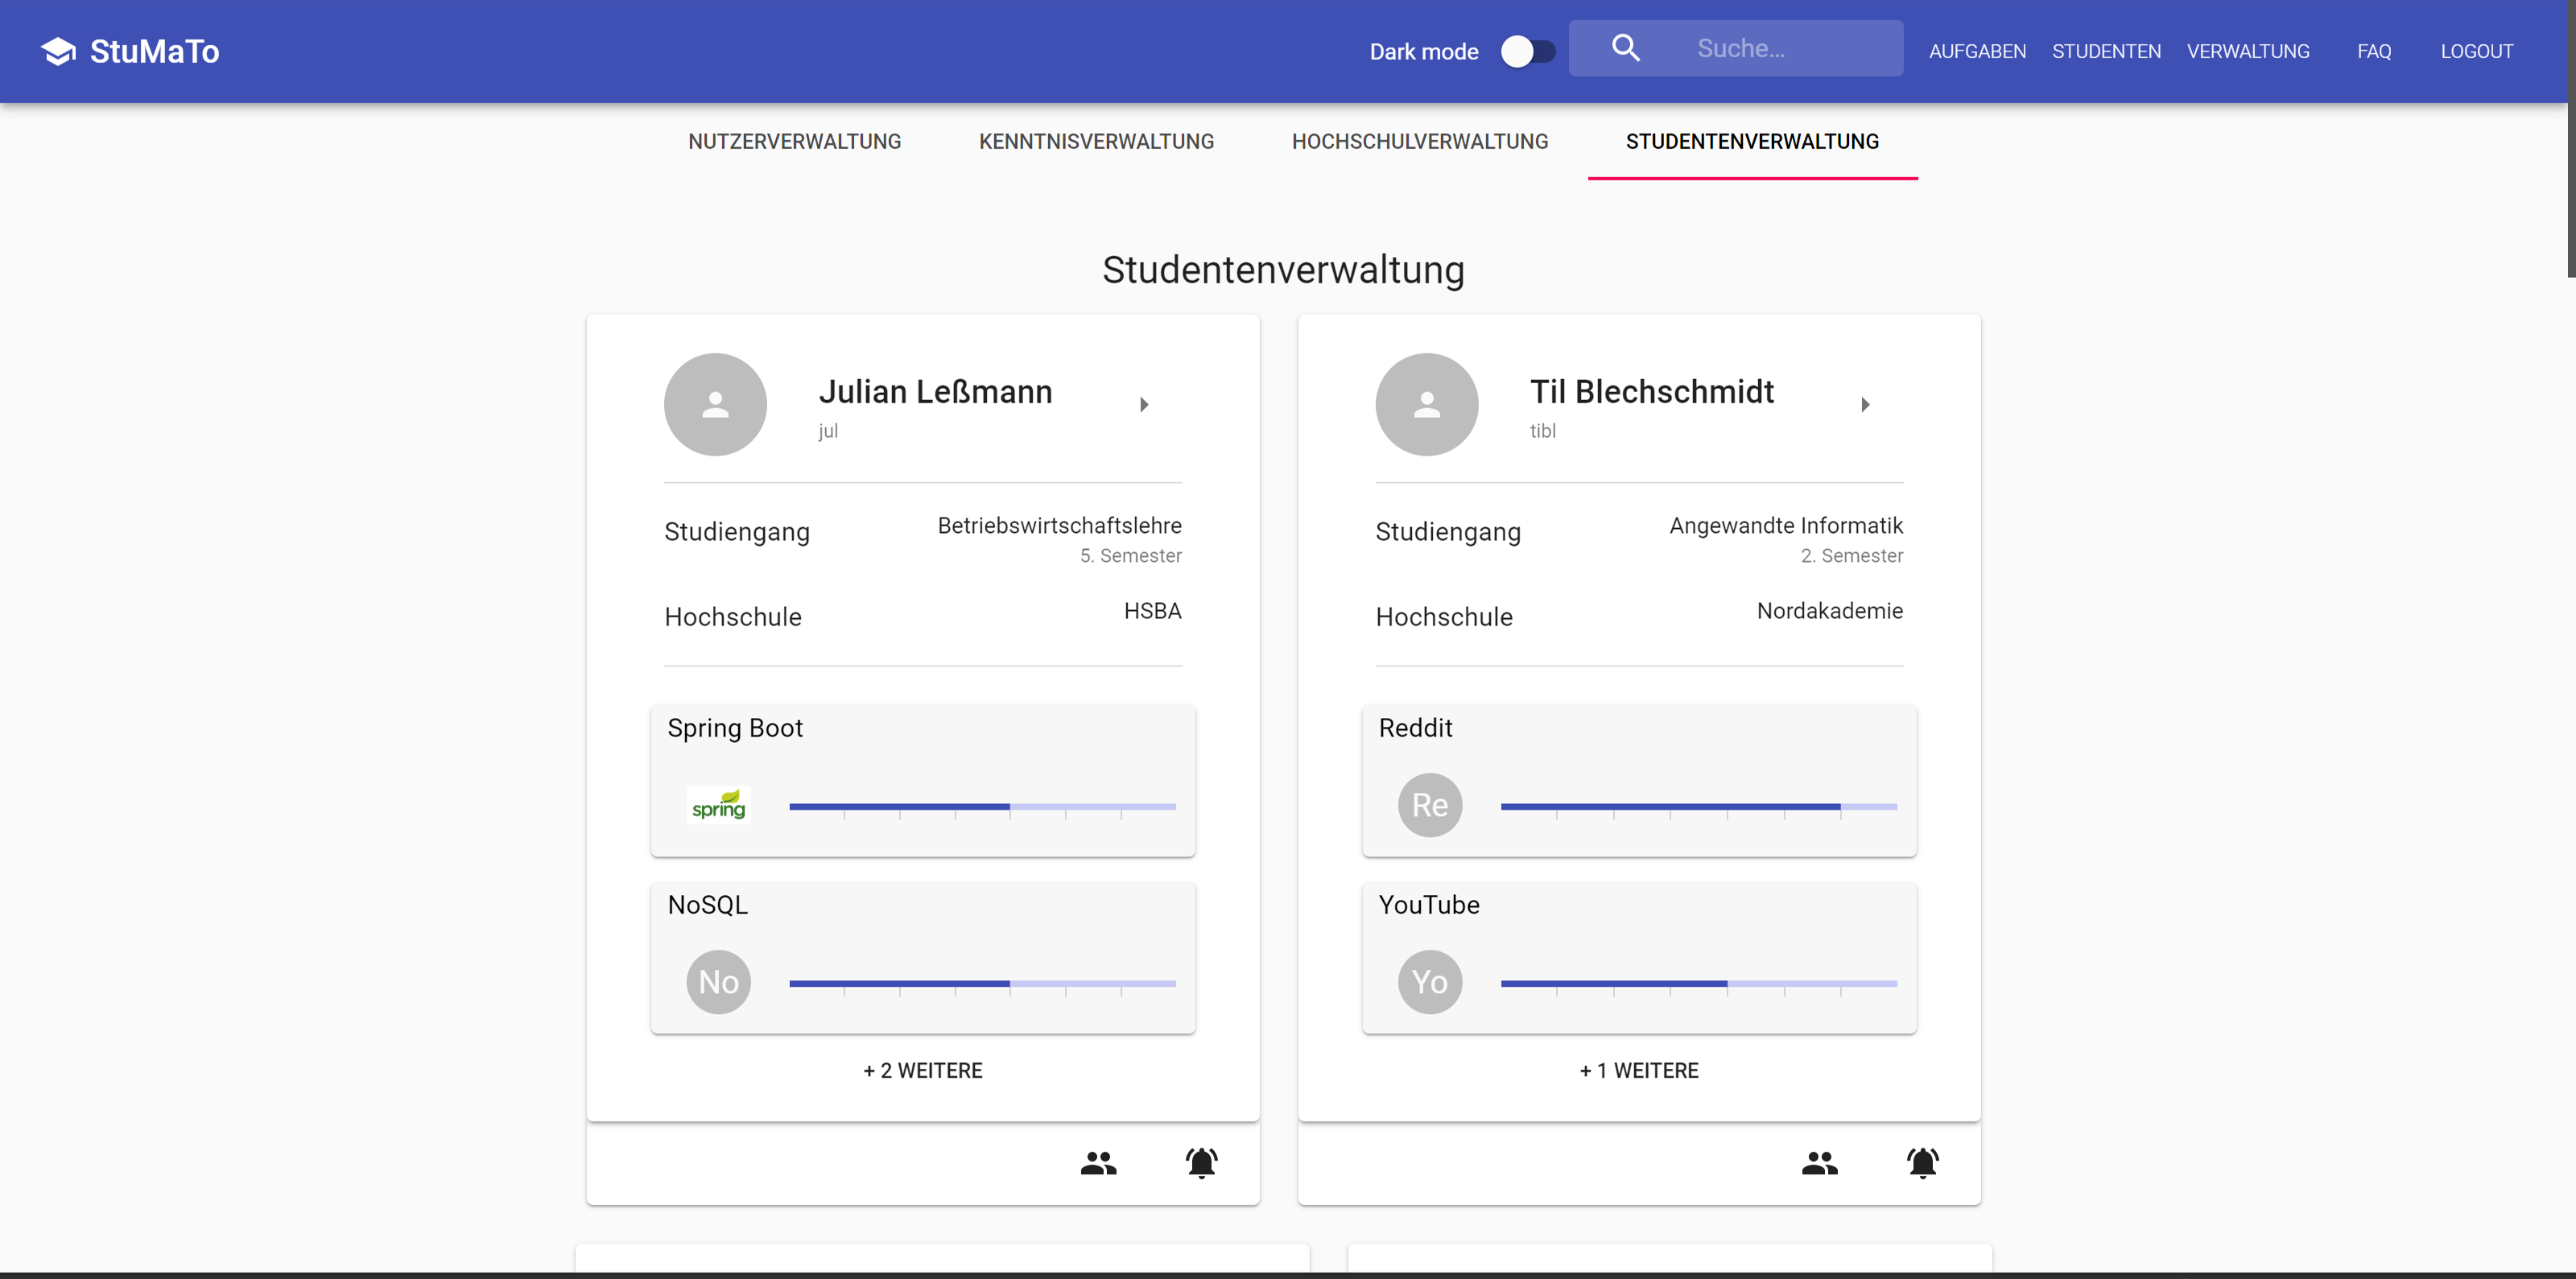
\includegraphics{./tex2pdf.-c803d322dfea80aa/829b0f3718891f438baaea67cf289ebd999fa92d.png}
\caption{Ansicht MANAGE.STUDENTS}
\end{figure}

\begin{figure}
\centering
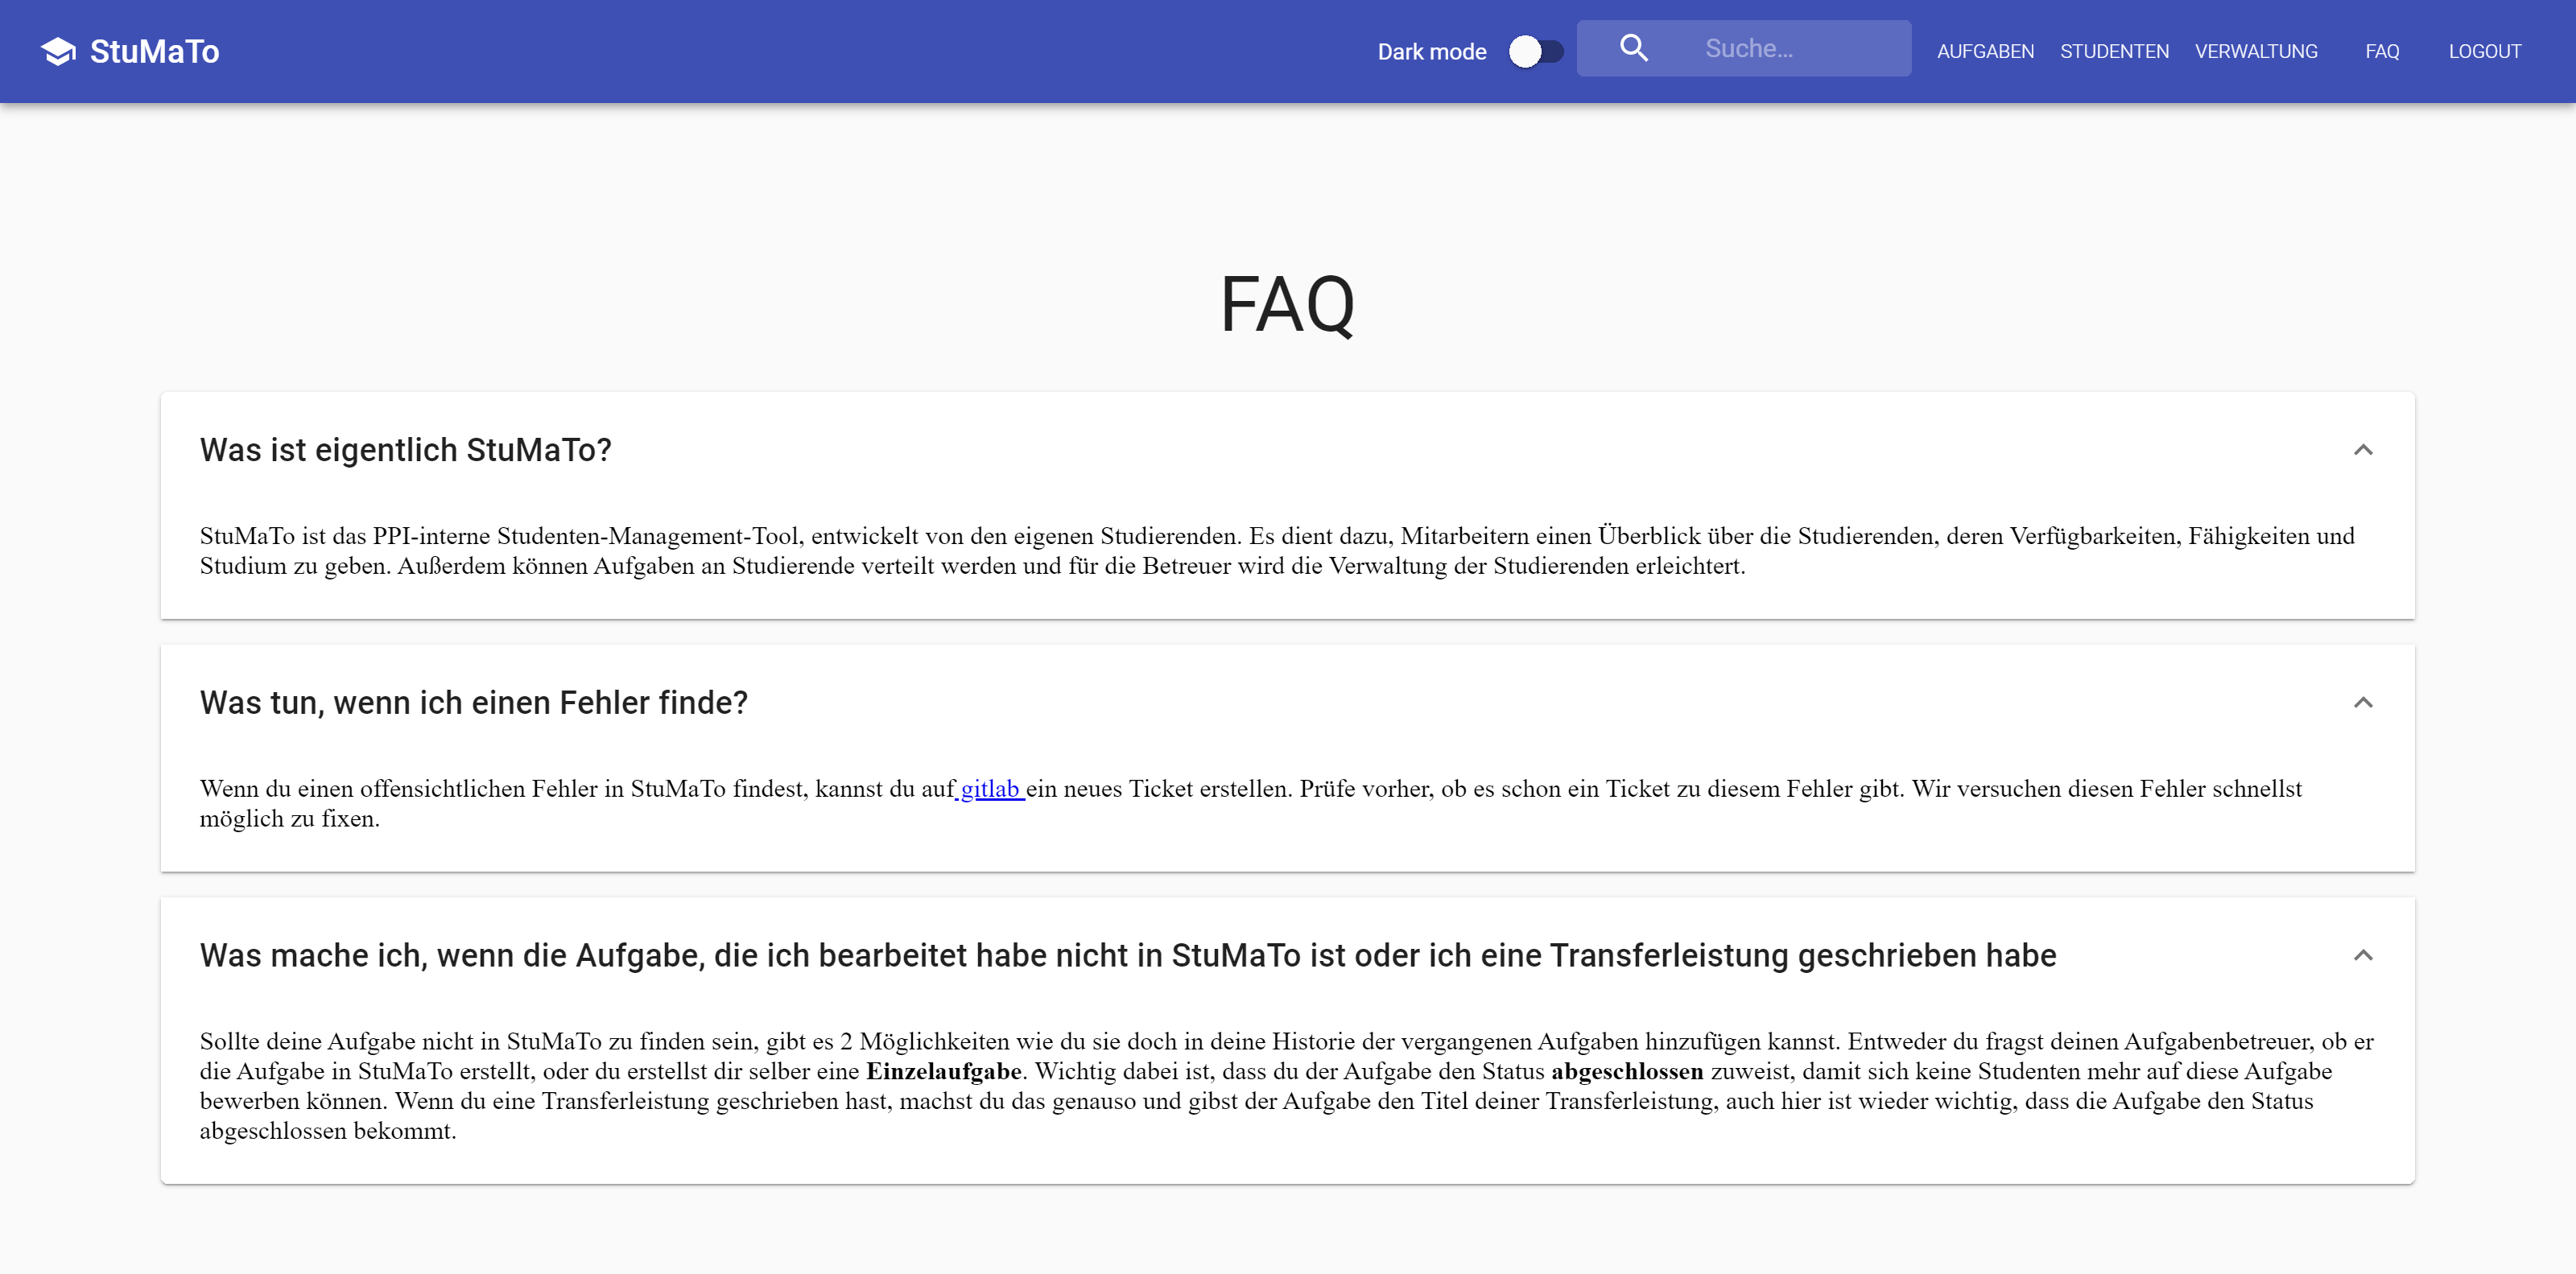
\includegraphics{./tex2pdf.-c803d322dfea80aa/9ec75c8fe138681c3d2ae6b2dae0f67a3a0aeba6.png}
\caption{Ansicht FAQ}
\end{figure}

\begin{figure}
\centering
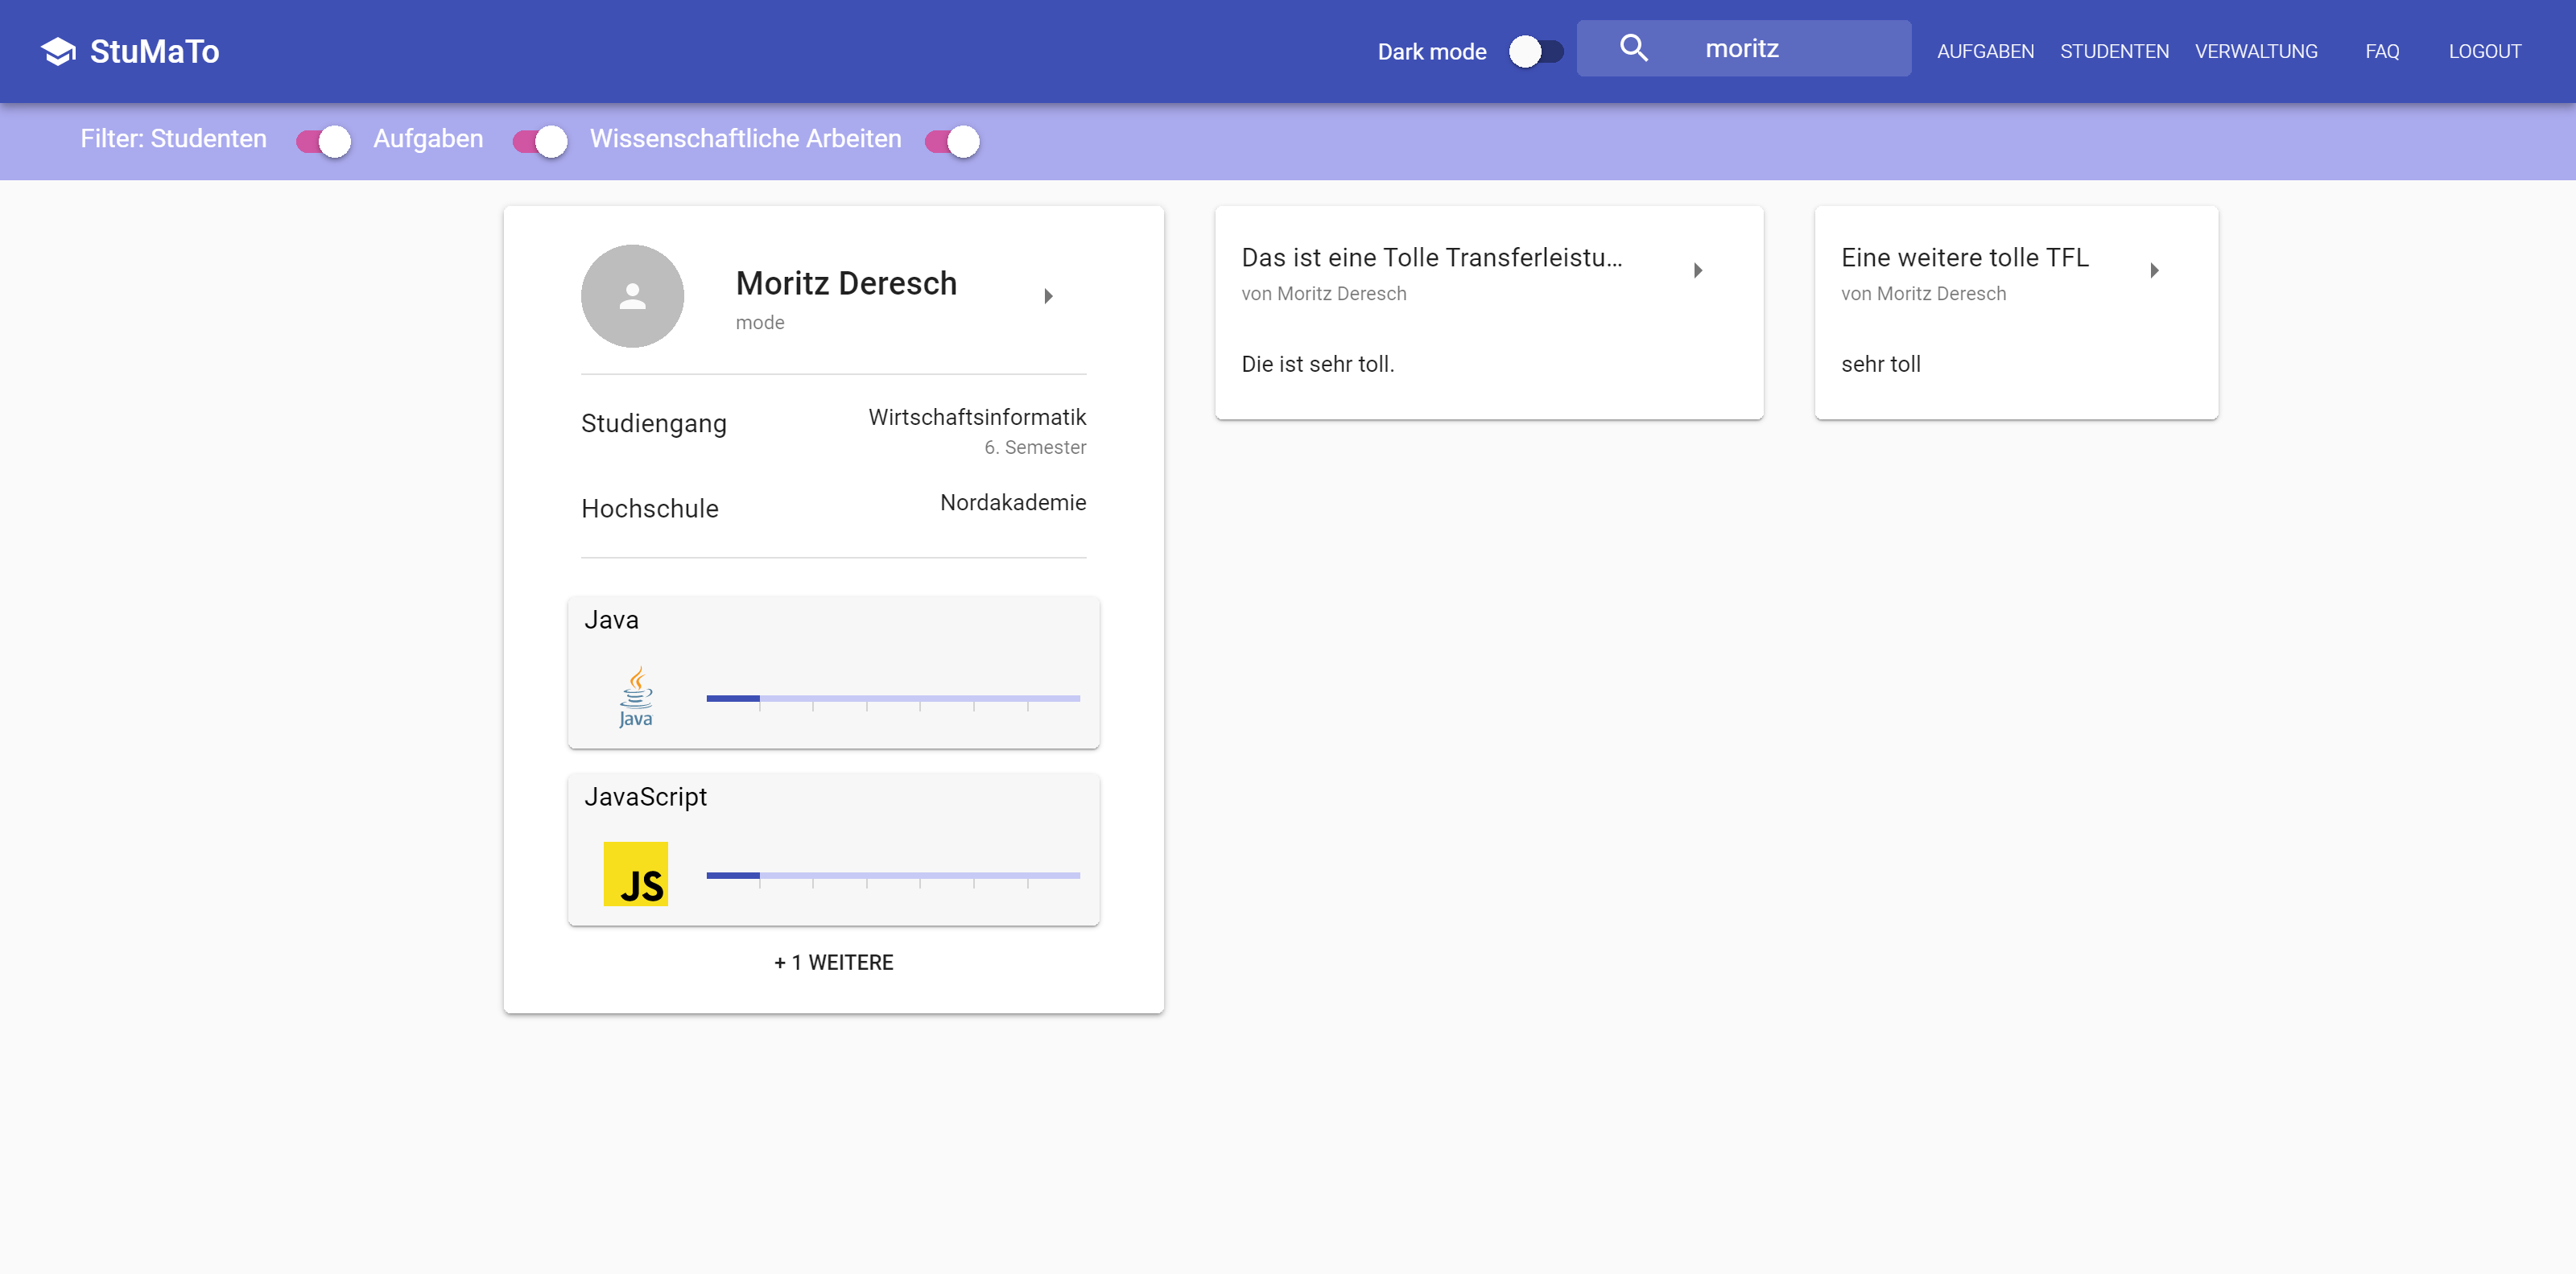
\includegraphics{./tex2pdf.-c803d322dfea80aa/b8df625acab593f077a2984960b30c10283f420a.png}
\caption{Ansicht SEARCH}
\end{figure}

\hypertarget{sec:heuristik-beschreibungen}{%
\subsection{Heuristik-Beschreibungen}\label{sec:heuristik-beschreibungen}}

\hypertarget{sec:heuristiken-shneiderman}{%
\subsubsection{Heuristiken nach
Shneiderman}\label{sec:heuristiken-shneiderman}}

Die folgenden Heuristiken nach Shneiderman wurden aus
{[}\protect\hyperlink{ref-heur:shneiderman}{2}{]} übernommen.

\begin{enumerate}
\def\labelenumi{\arabic{enumi}.}
\item
  \textbf{Strive for consistency.} Consistent sequences of actions
  should be required in similar situations; identical terminology should
  be used in prompts, menus, and help screens; and consistent color,
  layout, capitalization, fonts, and so on, should be employed
  throughout. Exceptions, such as required confirmation of the delete
  command or no echoing of passwords, should be comprehensible and
  limited in number
\item
  \textbf{Seek universal usability.} Recognize the needs of diverse
  users and design for plasticity, facilitating transformation of
  content. Novice to expert differences, age ranges, disabilities,
  international variations, and technological diversity each enrich the
  spectrum of requirements that guides design. Adding features for
  novices, such as explanations, and features for experts, such as
  shortcuts and faster pacing, enriches the interface design and
  improves perceived quality.
\item
  \textbf{Offer informative feedback.} For every user action, there
  should be an interface feedback. For frequent and minor actions, the
  response can be modest, whereas for infrequent and major actions, the
  response should be more substantial. Visual presentation of the
  objects of interest provides a convenient environment for showing
  changes explicitly (see the discussion of direct manipulation in
  Chapter 7).
\item
  \textbf{Design dialogs to yield closure.} Sequences of actions should
  be organized into groups with a beginning, middle, and end.
  Informative feedback at the completion of a group of actions gives
  users the satisfaction of accomplishment, a sense of relief, a signal
  to drop contingency plans from their minds, and an indicator to
  prepare for the next group of actions. For example, e-commerce
  websites move users from selecting products to the checkout, ending
  with a clear confirmation page that completes the transaction.
\item
  \textbf{Prevent errors.} As much as possible, design the interface so
  that users cannot make serious errors; for example, gray out menu
  items that are not appropriate and do not allow alphabetic characters
  in numeric entry fields (Section 3.3.5). If users make an error, the
  interface should offer simple, constructive, and specific instructions
  for recovery. For example, users should not have to retype an entire
  name-address form if they enter an invalid zip code but rather should
  be guided to repair only the faulty part. Erroneous actions should
  leave the interface state unchanged, or the interface should give
  instructions about restoring the state.
\item
  \textbf{Permit easy reversal of actions.} As much as possible, actions
  should be reversible. This feature relieves anxiety, since users know
  that errors can be undone, and encourages exploration of unfamiliar
  options. The units of reversibility may be a single action, a
  data-entry task, or a complete group of actions, such as entry of a
  name-address block.
\item
  \textbf{Keep users in control.} Experienced users strongly desire the
  sense that they are in charge of the interface and that the interface
  responds to their actions. They don't want surprises or changes in
  familiar behavior, and they are annoyed by tedious data-entry
  sequences, difficulty in obtaining necessary information, and
  inability to produce their desired result.
\item
  \textbf{Reduce short-term memory load.} Humans' limited capacity for
  information processing in short-term memory (the rule of thumb is that
  people can remember ``seven plus or minus two chunks'' of information)
  requires that designers avoid interfaces in which users must remember
  information from one display and then use that information on another
  display. It means that cellphones should not require reentry of phone
  numbers, website locations should remain visible, and lengthy forms
  should be compacted to fit a single display.
\end{enumerate}

\hypertarget{sec:heuristiken-nielsen}{%
\subsubsection{Heuristiken nach Nielsen}\label{sec:heuristiken-nielsen}}

Die folgenden Heuristiken nach Nielsen wurden aus
{[}\protect\hyperlink{ref-heur:nielsen}{3}{]} übernommen.

\begin{enumerate}
\def\labelenumi{\arabic{enumi}.}
\item
  \textbf{Visibility of system status} The system should always keep
  users informed about what is going on, through appropriate feedback
  within reasonable time.
\item
  \textbf{Match between system and the real world} The system should
  speak the users' language, with words, phrases and concepts familiar
  to the user, rather than system-oriented terms. Follow real-world
  conventions, making information appear in a natural and logical order.
\item
  \textbf{User control and freedom} Users often choose system functions
  by mistake and will need a clearly marked ``emergency exit'' to leave
  the unwanted state without having to go through an extended dialogue.
  Support undo and redo.
\item
  \textbf{Consistency and standards} Users should not have to wonder
  whether different words, situations, or actions mean the same thing.
  Follow platform conventions.
\item
  \textbf{Error prevention} Even better than good error messages is a
  careful design which prevents a problem from occurring in the first
  place. Either eliminate error-prone conditions or check for them and
  present users with a confirmation option before they commit to the
  action.
\item
  \textbf{Recognition rather than recall} Minimize the user's memory
  load by making objects, actions, and options visible. The user should
  not have to remember information from one part of the dialogue to
  another. Instructions for use of the system should be visible or
  easily retrievable whenever appropriate.
\item
  \textbf{Flexibility and efficiency of use} Accelerators -- unseen by
  the novice user -- may often speed up the interaction for the expert
  user such that the system can cater to both inexperienced and
  experienced users. Allow users to tailor frequent actions.
\item
  \textbf{Aesthetic and minimalist design} Dialogues should not contain
  information which is irrelevant or rarely needed. Every extra unit of
  information in a dialogue competes with the relevant units of
  information and diminishes their relative visibility.
\item
  \textbf{Help users recognize, diagnose, and recover from errors} Error
  messages should be expressed in plain language (no codes), precisely
  indicate the problem, and constructively suggest a solution.
\item
  \textbf{Help and documentation} Even though it is better if the system
  can be used without documentation, it may be necessary to provide help
  and documentation. Any such information should be easy to search,
  focused on the user's task, list concrete steps to be carried out, and
  not be too large.
\end{enumerate}

\hypertarget{sec:heuristik-rohergebnisse}{%
\subsection{Rohergebnisse der Heuristischen
Evaluation}\label{sec:heuristik-rohergebnisse}}

\hypertarget{problemfunde-je-evaluator}{%
\subsubsection{Problemfunde je
Evaluator}\label{problemfunde-je-evaluator}}

\hypertarget{hans}{%
\paragraph{Hans}\label{hans}}

\begin{longtable}[]{@{}lll@{}}
\caption{Problemfunde Hans \label{tbl:heur:hans}}\tabularnewline
\toprule
\begin{minipage}[b]{0.22\columnwidth}\raggedright
Kriterium\strut
\end{minipage} & \begin{minipage}[b]{0.52\columnwidth}\raggedright
Problem\strut
\end{minipage} & \begin{minipage}[b]{0.17\columnwidth}\raggedright
Fundort\strut
\end{minipage}\tabularnewline
\midrule
\endfirsthead
\toprule
\begin{minipage}[b]{0.22\columnwidth}\raggedright
Kriterium\strut
\end{minipage} & \begin{minipage}[b]{0.52\columnwidth}\raggedright
Problem\strut
\end{minipage} & \begin{minipage}[b]{0.17\columnwidth}\raggedright
Fundort\strut
\end{minipage}\tabularnewline
\midrule
\endhead
\begin{minipage}[t]{0.22\columnwidth}\raggedright
ADAPT\strut
\end{minipage} & \begin{minipage}[t]{0.52\columnwidth}\raggedright
Kontraste im dunklen Modus sind häufig schlecht, Beispiele dafür sind
der Dark-Mode-Schalter selbst, Lade-Spinner oder die Kennzeichnung
aktuell ausgewählter Tabs.\strut
\end{minipage} & \begin{minipage}[t]{0.17\columnwidth}\raggedright
*\strut
\end{minipage}\tabularnewline
\begin{minipage}[t]{0.22\columnwidth}\raggedright
ADAPT\strut
\end{minipage} & \begin{minipage}[t]{0.52\columnwidth}\raggedright
Viele UI-Elemente basieren pur auf Icons ohne Schrift, selbst ohne
Hovertexte. Das ist für Nutzer, die nicht mit der Symbolik vertraut
sind, oder sich aufgrund körperlicher Einschränkungen auf Screenreader
verlassen, ein Erschwernis. (Z.B. häufig hinzufügen, editieren,
etc.)\strut
\end{minipage} & \begin{minipage}[t]{0.17\columnwidth}\raggedright
z.B. TASKS.*\strut
\end{minipage}\tabularnewline
\begin{minipage}[t]{0.22\columnwidth}\raggedright
ADAPT\strut
\end{minipage} & \begin{minipage}[t]{0.52\columnwidth}\raggedright
Es gibt keine Anpassungsmöglichkeiten außerhalb des Farbschemas, der
Nutzer kann zum Beispiel Layouts, graphische Optionen oder ähnliches
nicht an sich anpassen.\strut
\end{minipage} & \begin{minipage}[t]{0.17\columnwidth}\raggedright
*\strut
\end{minipage}\tabularnewline
\begin{minipage}[t]{0.22\columnwidth}\raggedright
ADAPT\strut
\end{minipage} & \begin{minipage}[t]{0.52\columnwidth}\raggedright
Es existieren keine beschleunigenden Features für Experten. Es
existieren allgemein keine Tastaturkürzel für Aktionen.\strut
\end{minipage} & \begin{minipage}[t]{0.17\columnwidth}\raggedright
*\strut
\end{minipage}\tabularnewline
\begin{minipage}[t]{0.22\columnwidth}\raggedright
ADAPT\strut
\end{minipage} & \begin{minipage}[t]{0.52\columnwidth}\raggedright
Bei abweichender Bildschirmgröße sind Inhalte häufig außerhalb des
initialen Bildschirms und es muss gescrollt werden und die Anwendung ist
nicht für mobile Anwendungen optimiert.\strut
\end{minipage} & \begin{minipage}[t]{0.17\columnwidth}\raggedright
*\strut
\end{minipage}\tabularnewline
\begin{minipage}[t]{0.22\columnwidth}\raggedright
CLOSURE\strut
\end{minipage} & \begin{minipage}[t]{0.52\columnwidth}\raggedright
Das Speichern von Credit Points gibt wenig Feedback bei der Bestätigung
der Eingabe. Insgesamt ist es schwer ersichtlich, dass man die Eingabe
noch manuell abschließen muss, der Prozess ist nicht atomar.\strut
\end{minipage} & \begin{minipage}[t]{0.17\columnwidth}\raggedright
STUDENT.UNI\strut
\end{minipage}\tabularnewline
\begin{minipage}[t]{0.22\columnwidth}\raggedright
CLOSURE/STATUS\strut
\end{minipage} & \begin{minipage}[t]{0.52\columnwidth}\raggedright
Feedback zu erfolgreichen Aktionen teilweise schwer mitzubekommen oder
gar nicht existent. (z.B. Kenntnisse speichern)\strut
\end{minipage} & \begin{minipage}[t]{0.17\columnwidth}\raggedright
STUDENT.WORK\strut
\end{minipage}\tabularnewline
\begin{minipage}[t]{0.22\columnwidth}\raggedright
CONSIST\strut
\end{minipage} & \begin{minipage}[t]{0.52\columnwidth}\raggedright
FAQ und Dateinamen verwenden eine andere Schriftart als der Rest der
Anwendung.\strut
\end{minipage} & \begin{minipage}[t]{0.17\columnwidth}\raggedright
FAQ, STUDENT.UNI\strut
\end{minipage}\tabularnewline
\begin{minipage}[t]{0.22\columnwidth}\raggedright
CONSIST\strut
\end{minipage} & \begin{minipage}[t]{0.52\columnwidth}\raggedright
Einige GUI-Elemente, sind speziell für die Anwendung entwickelt worden
und sind nicht direkt intuitiv, sondern leicht verwirrend. (z.B. das
Widget zur Bearbeitung der Credit-Points)\strut
\end{minipage} & \begin{minipage}[t]{0.17\columnwidth}\raggedright
STUDENT.UNI\strut
\end{minipage}\tabularnewline
\begin{minipage}[t]{0.22\columnwidth}\raggedright
CONSIST\strut
\end{minipage} & \begin{minipage}[t]{0.52\columnwidth}\raggedright
Der Slider für Skills startet nicht ganz links und endet nicht ganz
rechts. Dies ist leicht irritierend, da man vermuten kann, ein
Bedienungsfehler wäre aufgetreten.\strut
\end{minipage} & \begin{minipage}[t]{0.17\columnwidth}\raggedright
STUDENT.WORK\strut
\end{minipage}\tabularnewline
\begin{minipage}[t]{0.22\columnwidth}\raggedright
CONTROL\strut
\end{minipage} & \begin{minipage}[t]{0.52\columnwidth}\raggedright
Die Verfügbarkeitssicht startet am Beginn der Aufzeichnung und nicht an
einem vom Nutzer bestimmten Punkt bzw. am heutigen Datum. Es muss jedes
Mal mühselig vorgescrollt werden.\strut
\end{minipage} & \begin{minipage}[t]{0.17\columnwidth}\raggedright
STUDENT.WORK\strut
\end{minipage}\tabularnewline
\begin{minipage}[t]{0.22\columnwidth}\raggedright
CONTROL\strut
\end{minipage} & \begin{minipage}[t]{0.52\columnwidth}\raggedright
Die Suchfilter sind nicht sofort verständlich in ihrer Bedeutung. Sie
setzen sich bei einer neuen Sucheingabe zurück.\strut
\end{minipage} & \begin{minipage}[t]{0.17\columnwidth}\raggedright
SEARCH\strut
\end{minipage}\tabularnewline
\begin{minipage}[t]{0.22\columnwidth}\raggedright
CONTROL\strut
\end{minipage} & \begin{minipage}[t]{0.52\columnwidth}\raggedright
Ein Klick auf einen Skill führt ohne Vorwarnung oder Kennzeichnung eine
Weiterleitung auf externe Websites, welche von Nutzern angegeben
werden.\strut
\end{minipage} & \begin{minipage}[t]{0.17\columnwidth}\raggedright
TASK.VIEW\strut
\end{minipage}\tabularnewline
\begin{minipage}[t]{0.22\columnwidth}\raggedright
CONTROL\strut
\end{minipage} & \begin{minipage}[t]{0.52\columnwidth}\raggedright
Eingetragene TFLs können nicht editiert, sondern nur neu angelegt
werden.\strut
\end{minipage} & \begin{minipage}[t]{0.17\columnwidth}\raggedright
STUDENT.UNI\strut
\end{minipage}\tabularnewline
\begin{minipage}[t]{0.22\columnwidth}\raggedright
ERR-HANDLE\strut
\end{minipage} & \begin{minipage}[t]{0.52\columnwidth}\raggedright
Wenn benötigte Felder in der Aufgabenerstellung ausgelassen werden, so
zeigt die Fehlermeldung nicht direkt, welche Felder noch gefüllt werden
müssen, sondern nur, dass Eingaben fehlen.\strut
\end{minipage} & \begin{minipage}[t]{0.17\columnwidth}\raggedright
TASK.EDIT\strut
\end{minipage}\tabularnewline
\begin{minipage}[t]{0.22\columnwidth}\raggedright
ERR-HANDLE\strut
\end{minipage} & \begin{minipage}[t]{0.52\columnwidth}\raggedright
Bei einem provozierten Fehler wurde kontinuierlich gespeichert, ein
Abbrechen war nicht möglich oder keine Fehlermeldung wurde angezeigt.
(Hochladen von Dateien)\strut
\end{minipage} & \begin{minipage}[t]{0.17\columnwidth}\raggedright
STUDENT.UNI.NEW-TFL\strut
\end{minipage}\tabularnewline
\begin{minipage}[t]{0.22\columnwidth}\raggedright
ERR-HANDLE / STATUS\strut
\end{minipage} & \begin{minipage}[t]{0.52\columnwidth}\raggedright
Bei dem Versuch der Erstellung einer Hochschule ohne Namen kommt ein
intransparenter, langer Ladevorgang ohne anschließende
Misserfolgsmeldung.\strut
\end{minipage} & \begin{minipage}[t]{0.17\columnwidth}\raggedright
MANAGE.UNI\strut
\end{minipage}\tabularnewline
\begin{minipage}[t]{0.22\columnwidth}\raggedright
ERR-PREV\strut
\end{minipage} & \begin{minipage}[t]{0.52\columnwidth}\raggedright
Benötigte Felder in der Aufgabenerstellung werden nicht vorher
gekennzeichnet.\strut
\end{minipage} & \begin{minipage}[t]{0.17\columnwidth}\raggedright
TASK.EDIT\strut
\end{minipage}\tabularnewline
\begin{minipage}[t]{0.22\columnwidth}\raggedright
ERR-PREV\strut
\end{minipage} & \begin{minipage}[t]{0.52\columnwidth}\raggedright
Kein Nachfragen wenn geänderte Aufgabe nicht gespeichert und dann
abgebrochen wird\strut
\end{minipage} & \begin{minipage}[t]{0.17\columnwidth}\raggedright
TASK.EDIT\strut
\end{minipage}\tabularnewline
\begin{minipage}[t]{0.22\columnwidth}\raggedright
ERR-PREV\strut
\end{minipage} & \begin{minipage}[t]{0.52\columnwidth}\raggedright
Notwendige Felder beim Anlegen von Aufgaben erst im Nachhinein
angezeigt\strut
\end{minipage} & \begin{minipage}[t]{0.17\columnwidth}\raggedright
TASK.EDIT\strut
\end{minipage}\tabularnewline
\begin{minipage}[t]{0.22\columnwidth}\raggedright
ERR-PREV\strut
\end{minipage} & \begin{minipage}[t]{0.52\columnwidth}\raggedright
Aktionsbuttons werden häufig mit Aktionen wie ``ok'' betitelt, eine
sprechende Bezeichnung der Aktion, die folgt, wäre besser.\strut
\end{minipage} & \begin{minipage}[t]{0.17\columnwidth}\raggedright
*\strut
\end{minipage}\tabularnewline
\begin{minipage}[t]{0.22\columnwidth}\raggedright
ERR-PREV\strut
\end{minipage} & \begin{minipage}[t]{0.52\columnwidth}\raggedright
Bei editierten Credit Points oder Kenntnissen im Profil keine Nachfrage
beim Verlassen der Seite\strut
\end{minipage} & \begin{minipage}[t]{0.17\columnwidth}\raggedright
STUDENT.WORK\strut
\end{minipage}\tabularnewline
\begin{minipage}[t]{0.22\columnwidth}\raggedright
HELP\strut
\end{minipage} & \begin{minipage}[t]{0.52\columnwidth}\raggedright
Kaum nützliche Hover-Texte.\strut
\end{minipage} & \begin{minipage}[t]{0.17\columnwidth}\raggedright
*\strut
\end{minipage}\tabularnewline
\begin{minipage}[t]{0.22\columnwidth}\raggedright
HELP\strut
\end{minipage} & \begin{minipage}[t]{0.52\columnwidth}\raggedright
Kein abrufbarer Hilfe-Dialog, FAQ ist dürftig.\strut
\end{minipage} & \begin{minipage}[t]{0.17\columnwidth}\raggedright
FAQ\strut
\end{minipage}\tabularnewline
\begin{minipage}[t]{0.22\columnwidth}\raggedright
HELP\strut
\end{minipage} & \begin{minipage}[t]{0.52\columnwidth}\raggedright
Es ist nicht immer klar beschrieben, welche Konsequenzen eine Aktion
hat.\strut
\end{minipage} & \begin{minipage}[t]{0.17\columnwidth}\raggedright
*\strut
\end{minipage}\tabularnewline
\begin{minipage}[t]{0.22\columnwidth}\raggedright
REAL\strut
\end{minipage} & \begin{minipage}[t]{0.52\columnwidth}\raggedright
Alumni \& Alumnae ist ein selten verwendeter Begriff, neue Studenten
können damit vielleicht nicht viel anfangen.\strut
\end{minipage} & \begin{minipage}[t]{0.17\columnwidth}\raggedright
STUDENT.LIST\strut
\end{minipage}\tabularnewline
\begin{minipage}[t]{0.22\columnwidth}\raggedright
REAL\strut
\end{minipage} & \begin{minipage}[t]{0.52\columnwidth}\raggedright
Icons für offene / angefangen Aufgaben sind unbekannt und transportieren
keine klare Nachricht.\strut
\end{minipage} & \begin{minipage}[t]{0.17\columnwidth}\raggedright
TASK.VIEW\strut
\end{minipage}\tabularnewline
\begin{minipage}[t]{0.22\columnwidth}\raggedright
REAL\strut
\end{minipage} & \begin{minipage}[t]{0.52\columnwidth}\raggedright
Die Bezeichnungen der Aufgabenkategorien haben keine klare Beziehung zum
echten Leben. Wie lange dauern Einzel- vs.~Daueraufgaben? Warum werden
nur offene Aufgaben angezeigt? Wo ist das Archiv? (AW: in ``Alle
Aufgaben'')\strut
\end{minipage} & \begin{minipage}[t]{0.17\columnwidth}\raggedright
TASK.*\strut
\end{minipage}\tabularnewline
\begin{minipage}[t]{0.22\columnwidth}\raggedright
RECOG\strut
\end{minipage} & \begin{minipage}[t]{0.52\columnwidth}\raggedright
Es ist z.B. nicht mehr klar, welches Profil gerade editiert wird, wenn
ein Editierdialog offen ist.\strut
\end{minipage} & \begin{minipage}[t]{0.17\columnwidth}\raggedright
STUDENT.*\strut
\end{minipage}\tabularnewline
\begin{minipage}[t]{0.22\columnwidth}\raggedright
RECOG / STATUS / ERR-PREV\strut
\end{minipage} & \begin{minipage}[t]{0.52\columnwidth}\raggedright
Nicht abzusehen ob eine editierte Aufgabe,CP,Kenntnisse bereits
gespeichert oder noch ``dirty'' ist.\strut
\end{minipage} & \begin{minipage}[t]{0.17\columnwidth}\raggedright
STUDENT.*\strut
\end{minipage}\tabularnewline
\begin{minipage}[t]{0.22\columnwidth}\raggedright
RELEV\strut
\end{minipage} & \begin{minipage}[t]{0.52\columnwidth}\raggedright
Die potentiell etwas längere Kurzbeschreibung bläht das Layout auf. Der
Titel würde hier reichen.\strut
\end{minipage} & \begin{minipage}[t]{0.17\columnwidth}\raggedright
STUDENT.UNI\strut
\end{minipage}\tabularnewline
\begin{minipage}[t]{0.22\columnwidth}\raggedright
RELEV\strut
\end{minipage} & \begin{minipage}[t]{0.52\columnwidth}\raggedright
Credit Points werden auch dann angezeigt, wenn keine Daten vorhanden
sind (auch auf fremden Profilen)\strut
\end{minipage} & \begin{minipage}[t]{0.17\columnwidth}\raggedright
STUDENT.UNI\strut
\end{minipage}\tabularnewline
\begin{minipage}[t]{0.22\columnwidth}\raggedright
RELEV\strut
\end{minipage} & \begin{minipage}[t]{0.52\columnwidth}\raggedright
Leere Timeline, leere Kenntnisse etc. werden angezeigt, ohne Mehrwert zu
erbringen.\strut
\end{minipage} & \begin{minipage}[t]{0.17\columnwidth}\raggedright
STUDENT.UNI\strut
\end{minipage}\tabularnewline
\begin{minipage}[t]{0.22\columnwidth}\raggedright
RELEV\strut
\end{minipage} & \begin{minipage}[t]{0.52\columnwidth}\raggedright
Aufgaben können nicht nach (eigenen) Kenntnissen gefiltert werden\strut
\end{minipage} & \begin{minipage}[t]{0.17\columnwidth}\raggedright
TASK.*, SEARCH\strut
\end{minipage}\tabularnewline
\begin{minipage}[t]{0.22\columnwidth}\raggedright
RELEV\strut
\end{minipage} & \begin{minipage}[t]{0.52\columnwidth}\raggedright
Zu jedem Studenten wird zusätzlich ein unnützes Nutzerkürzel
angezeigt.\strut
\end{minipage} & \begin{minipage}[t]{0.17\columnwidth}\raggedright
STUDENT.*, MANAGE.*\strut
\end{minipage}\tabularnewline
\begin{minipage}[t]{0.22\columnwidth}\raggedright
STATUS\strut
\end{minipage} & \begin{minipage}[t]{0.52\columnwidth}\raggedright
Es gibt keinen schnellen Indikator für den eingeloggten Benutzer.\strut
\end{minipage} & \begin{minipage}[t]{0.17\columnwidth}\raggedright
*\strut
\end{minipage}\tabularnewline
\begin{minipage}[t]{0.22\columnwidth}\raggedright
STATUS\strut
\end{minipage} & \begin{minipage}[t]{0.52\columnwidth}\raggedright
Es ist leicht zu übersehen, dass das Editieren von CP noch aktiv
ist.\strut
\end{minipage} & \begin{minipage}[t]{0.17\columnwidth}\raggedright
STUDENT.UNI\strut
\end{minipage}\tabularnewline
\begin{minipage}[t]{0.22\columnwidth}\raggedright
UNDO\strut
\end{minipage} & \begin{minipage}[t]{0.52\columnwidth}\raggedright
Keine Möglichkeit, Änderungen rückgängig zu machen oder auch nur
nachzuverfolgen\strut
\end{minipage} & \begin{minipage}[t]{0.17\columnwidth}\raggedright
*\strut
\end{minipage}\tabularnewline
\begin{minipage}[t]{0.22\columnwidth}\raggedright
UPTODATE / ERR-PREV\strut
\end{minipage} & \begin{minipage}[t]{0.52\columnwidth}\raggedright
Zeitlich abgelaufene Aufgaben wurden als verfügbar angezeigt, auch wenn
sie dezent als abgelaufen gekennzeichnet waren.\strut
\end{minipage} & \begin{minipage}[t]{0.17\columnwidth}\raggedright
TASK.*\strut
\end{minipage}\tabularnewline
\begin{minipage}[t]{0.22\columnwidth}\raggedright
UPTODATE / ERR-PREV\strut
\end{minipage} & \begin{minipage}[t]{0.52\columnwidth}\raggedright
Es existieren unmögliche Nutzerdaten, wie zum Beispiel ein Nutzer, der
seit 2017 Student, aber im 2. Semester ist, oder noch gravierender seit
2021 aber Student aber im 20. Semester. Hier fehlen Validierungen.\strut
\end{minipage} & \begin{minipage}[t]{0.17\columnwidth}\raggedright
STUDENT.*\strut
\end{minipage}\tabularnewline
\bottomrule
\end{longtable}

\hypertarget{hendrik}{%
\paragraph{Hendrik}\label{hendrik}}

\begin{longtable}[]{@{}lll@{}}
\caption{Problemfunde Hendrik \label{tbl:heur:hendrik}}\tabularnewline
\toprule
\begin{minipage}[b]{0.15\columnwidth}\raggedright
Kriterium\strut
\end{minipage} & \begin{minipage}[b]{0.49\columnwidth}\raggedright
Probleme\strut
\end{minipage} & \begin{minipage}[b]{0.27\columnwidth}\raggedright
Fundort\strut
\end{minipage}\tabularnewline
\midrule
\endfirsthead
\toprule
\begin{minipage}[b]{0.15\columnwidth}\raggedright
Kriterium\strut
\end{minipage} & \begin{minipage}[b]{0.49\columnwidth}\raggedright
Probleme\strut
\end{minipage} & \begin{minipage}[b]{0.27\columnwidth}\raggedright
Fundort\strut
\end{minipage}\tabularnewline
\midrule
\endhead
\begin{minipage}[t]{0.15\columnwidth}\raggedright
ADAPT\strut
\end{minipage} & \begin{minipage}[t]{0.49\columnwidth}\raggedright
Kontraste im Darkmode sind nicht gut, Elemente könnten übersehen
werden.\strut
\end{minipage} & \begin{minipage}[t]{0.27\columnwidth}\raggedright
MANAGE, TASK.*, FAQ, STUDENT.WORK\strut
\end{minipage}\tabularnewline
\begin{minipage}[t]{0.15\columnwidth}\raggedright
CLOSURE\strut
\end{minipage} & \begin{minipage}[t]{0.49\columnwidth}\raggedright
Bei Bearbeitung des Studentenprofils ist der Abschluss von Aufgaben
nicht klar, es kann ewig ohne klare Abfolge editiert werden.\strut
\end{minipage} & \begin{minipage}[t]{0.27\columnwidth}\raggedright
STUDENT.UNI, STUDENT.WORK\strut
\end{minipage}\tabularnewline
\begin{minipage}[t]{0.15\columnwidth}\raggedright
CLOSURE\strut
\end{minipage} & \begin{minipage}[t]{0.49\columnwidth}\raggedright
Das Verändern der Kenntnisse ruft keine Speicheroperation hervor und
durch eine Speicheroperation wird keine Rückmeldung hervorgerufen, die
die Aktion für den Nutzer abschließt\strut
\end{minipage} & \begin{minipage}[t]{0.27\columnwidth}\raggedright
STUDENT.WORK\strut
\end{minipage}\tabularnewline
\begin{minipage}[t]{0.15\columnwidth}\raggedright
CONSIST\strut
\end{minipage} & \begin{minipage}[t]{0.49\columnwidth}\raggedright
Die Webseite verwendet kein HTTPS, wodurch potentiell Unsicherheit
entsteht.\strut
\end{minipage} & \begin{minipage}[t]{0.27\columnwidth}\raggedright
*\strut
\end{minipage}\tabularnewline
\begin{minipage}[t]{0.15\columnwidth}\raggedright
CONSIST\strut
\end{minipage} & \begin{minipage}[t]{0.49\columnwidth}\raggedright
Aufgabenstatus sind auf Englisch, wenn der Rest der Anwendung auf
Deutsch ist\strut
\end{minipage} & \begin{minipage}[t]{0.27\columnwidth}\raggedright
TASK.*\strut
\end{minipage}\tabularnewline
\begin{minipage}[t]{0.15\columnwidth}\raggedright
CONSIST\strut
\end{minipage} & \begin{minipage}[t]{0.49\columnwidth}\raggedright
Studenten in den Aufgaben sehen aus, als könnte man sie anklicken, aber
nichts passiert danach\strut
\end{minipage} & \begin{minipage}[t]{0.27\columnwidth}\raggedright
TASK.VIEW\strut
\end{minipage}\tabularnewline
\begin{minipage}[t]{0.15\columnwidth}\raggedright
CONSIST\strut
\end{minipage} & \begin{minipage}[t]{0.49\columnwidth}\raggedright
Kenntnisse sehen beim Anlegen einer Aufgabe aus als wären sie
anklickbar.\strut
\end{minipage} & \begin{minipage}[t]{0.27\columnwidth}\raggedright
TASK.EDIT\strut
\end{minipage}\tabularnewline
\begin{minipage}[t]{0.15\columnwidth}\raggedright
CONTROL\strut
\end{minipage} & \begin{minipage}[t]{0.49\columnwidth}\raggedright
Die ``Verfügbarkeit''-Zeitlinie ist nicht auf das aktuelle Datum
gerichtet.\strut
\end{minipage} & \begin{minipage}[t]{0.27\columnwidth}\raggedright
STUDENT.UNI\strut
\end{minipage}\tabularnewline
\begin{minipage}[t]{0.15\columnwidth}\raggedright
CONTROL\strut
\end{minipage} & \begin{minipage}[t]{0.49\columnwidth}\raggedright
Es können nicht alle wissenschaftlichen Arbeiten auf einmal gesucht /
gefunden werden.\strut
\end{minipage} & \begin{minipage}[t]{0.27\columnwidth}\raggedright
*\strut
\end{minipage}\tabularnewline
\begin{minipage}[t]{0.15\columnwidth}\raggedright
CONTROL / RECOG\strut
\end{minipage} & \begin{minipage}[t]{0.49\columnwidth}\raggedright
Beim Anlegen eines neuen Kalendereintrags sind Aufgaben schwer
auffindbar und können nicht neu angelegt werden. Der Nutzer muss sich
den Namen der Aufgabe gemerkt haben.\strut
\end{minipage} & \begin{minipage}[t]{0.27\columnwidth}\raggedright
STUDENT.WORK.NEW-ENTRY\strut
\end{minipage}\tabularnewline
\begin{minipage}[t]{0.15\columnwidth}\raggedright
ERR-PREV\strut
\end{minipage} & \begin{minipage}[t]{0.49\columnwidth}\raggedright
Bei der Erstellung neuer Skills wird keine Validierung
vorgenommen.\strut
\end{minipage} & \begin{minipage}[t]{0.27\columnwidth}\raggedright
MANAGE.SKILLS\strut
\end{minipage}\tabularnewline
\begin{minipage}[t]{0.15\columnwidth}\raggedright
ERR-PREV / CONTROL\strut
\end{minipage} & \begin{minipage}[t]{0.49\columnwidth}\raggedright
Ich weiß nicht, was für eine Mail versendet wird, wenn ich auf Interesse
drücke.\strut
\end{minipage} & \begin{minipage}[t]{0.27\columnwidth}\raggedright
TASK.VIEW\strut
\end{minipage}\tabularnewline
\begin{minipage}[t]{0.15\columnwidth}\raggedright
HELP\strut
\end{minipage} & \begin{minipage}[t]{0.49\columnwidth}\raggedright
Bei Skills ist nicht klar, bei welchem Skill ich mich selber einordnen
soll, es existiert keine Dokumentation als Vergleichsreferenz.\strut
\end{minipage} & \begin{minipage}[t]{0.27\columnwidth}\raggedright
STUDENT.WORK\strut
\end{minipage}\tabularnewline
\begin{minipage}[t]{0.15\columnwidth}\raggedright
HELP\strut
\end{minipage} & \begin{minipage}[t]{0.49\columnwidth}\raggedright
Das FAQ ist nicht wirklich gut.\strut
\end{minipage} & \begin{minipage}[t]{0.27\columnwidth}\raggedright
FAQ\strut
\end{minipage}\tabularnewline
\begin{minipage}[t]{0.15\columnwidth}\raggedright
REAL\strut
\end{minipage} & \begin{minipage}[t]{0.49\columnwidth}\raggedright
Dauer-/Einzelaufgaben sind keine Worte aus der realen Welt, und sollen
eher Aufgaben vs.~Teams darstellen.\strut
\end{minipage} & \begin{minipage}[t]{0.27\columnwidth}\raggedright
TASK.SINGLE, TASK.PERM\strut
\end{minipage}\tabularnewline
\begin{minipage}[t]{0.15\columnwidth}\raggedright
REAL\strut
\end{minipage} & \begin{minipage}[t]{0.49\columnwidth}\raggedright
Creditpoints für ``Hausarbeiten'' stimmen nicht überein, da z.B. für
NAK-Studenten hier TFLs gemeint sind.\strut
\end{minipage} & \begin{minipage}[t]{0.27\columnwidth}\raggedright
STUDENT.UNI\strut
\end{minipage}\tabularnewline
\begin{minipage}[t]{0.15\columnwidth}\raggedright
RELEV\strut
\end{minipage} & \begin{minipage}[t]{0.49\columnwidth}\raggedright
Dashboardbuttons führen immer zum selben, wenn man nicht eingeloggt ist.
Die nicht funktionalen Buttons sind nicht notwendig.\strut
\end{minipage} & \begin{minipage}[t]{0.27\columnwidth}\raggedright
DASH1\strut
\end{minipage}\tabularnewline
\begin{minipage}[t]{0.15\columnwidth}\raggedright
STATUS\strut
\end{minipage} & \begin{minipage}[t]{0.49\columnwidth}\raggedright
Die Veränderung der Rolle eines Nutzers zieht keine Erfolgsmeldung nach
sich.\strut
\end{minipage} & \begin{minipage}[t]{0.27\columnwidth}\raggedright
MANAGE.USER\strut
\end{minipage}\tabularnewline
\begin{minipage}[t]{0.15\columnwidth}\raggedright
UNDO\strut
\end{minipage} & \begin{minipage}[t]{0.49\columnwidth}\raggedright
Ein Undo/Redo ist nicht möglich\strut
\end{minipage} & \begin{minipage}[t]{0.27\columnwidth}\raggedright
*\strut
\end{minipage}\tabularnewline
\begin{minipage}[t]{0.15\columnwidth}\raggedright
UPTODATE\strut
\end{minipage} & \begin{minipage}[t]{0.49\columnwidth}\raggedright
Keine Aufgaben sind im Startbereich zu sehen\strut
\end{minipage} & \begin{minipage}[t]{0.27\columnwidth}\raggedright
TASK.ALL\strut
\end{minipage}\tabularnewline
\begin{minipage}[t]{0.15\columnwidth}\raggedright
UPTODATE\strut
\end{minipage} & \begin{minipage}[t]{0.49\columnwidth}\raggedright
Ehemalige Studenten werden als Studenten geführt.\strut
\end{minipage} & \begin{minipage}[t]{0.27\columnwidth}\raggedright
STUDENT.LIST\strut
\end{minipage}\tabularnewline
\begin{minipage}[t]{0.15\columnwidth}\raggedright
UPTODSATE\strut
\end{minipage} & \begin{minipage}[t]{0.49\columnwidth}\raggedright
Profile sind wenig gepflegt.\strut
\end{minipage} & \begin{minipage}[t]{0.27\columnwidth}\raggedright
STUDENT.*\strut
\end{minipage}\tabularnewline
\begin{minipage}[t]{0.15\columnwidth}\raggedright
UPTODATE\strut
\end{minipage} & \begin{minipage}[t]{0.49\columnwidth}\raggedright
Standort von Aufgabe ist schlecht dokumentiert.\strut
\end{minipage} & \begin{minipage}[t]{0.27\columnwidth}\raggedright
TASK.*\strut
\end{minipage}\tabularnewline
\begin{minipage}[t]{0.15\columnwidth}\raggedright
UPTODATE\strut
\end{minipage} & \begin{minipage}[t]{0.49\columnwidth}\raggedright
Semesterangaben sind bei einigen Studenten um ein Semester
versetzt.\strut
\end{minipage} & \begin{minipage}[t]{0.27\columnwidth}\raggedright
STUDENT.UNI\strut
\end{minipage}\tabularnewline
\bottomrule
\end{longtable}

\hypertarget{til}{%
\paragraph{Til}\label{til}}

\begin{longtable}[]{@{}lll@{}}
\caption{Problemfunde Til \label{tbl:heur:til}}\tabularnewline
\toprule
\begin{minipage}[b]{0.14\columnwidth}\raggedright
Kriterium\strut
\end{minipage} & \begin{minipage}[b]{0.55\columnwidth}\raggedright
Probleme\strut
\end{minipage} & \begin{minipage}[b]{0.23\columnwidth}\raggedright
Fundort\strut
\end{minipage}\tabularnewline
\midrule
\endfirsthead
\toprule
\begin{minipage}[b]{0.14\columnwidth}\raggedright
Kriterium\strut
\end{minipage} & \begin{minipage}[b]{0.55\columnwidth}\raggedright
Probleme\strut
\end{minipage} & \begin{minipage}[b]{0.23\columnwidth}\raggedright
Fundort\strut
\end{minipage}\tabularnewline
\midrule
\endhead
\begin{minipage}[t]{0.14\columnwidth}\raggedright
ADAPT\strut
\end{minipage} & \begin{minipage}[t]{0.55\columnwidth}\raggedright
Keine Anpassbarkeit vorhanden.\strut
\end{minipage} & \begin{minipage}[t]{0.23\columnwidth}\raggedright
*\strut
\end{minipage}\tabularnewline
\begin{minipage}[t]{0.14\columnwidth}\raggedright
CONSIST\strut
\end{minipage} & \begin{minipage}[t]{0.55\columnwidth}\raggedright
Keine expliziten Speicher-Buttons an einigen Orten, an anderen
schon.\strut
\end{minipage} & \begin{minipage}[t]{0.23\columnwidth}\raggedright
STUDENT.*, MANAGE.*\strut
\end{minipage}\tabularnewline
\begin{minipage}[t]{0.14\columnwidth}\raggedright
CONSIST\strut
\end{minipage} & \begin{minipage}[t]{0.55\columnwidth}\raggedright
Layout (Spacings etc.) ist teilweise uneinheitlich.\strut
\end{minipage} & \begin{minipage}[t]{0.23\columnwidth}\raggedright
TASK.*\strut
\end{minipage}\tabularnewline
\begin{minipage}[t]{0.14\columnwidth}\raggedright
CONSIST\strut
\end{minipage} & \begin{minipage}[t]{0.55\columnwidth}\raggedright
Vertikale / Horizontale Einrückung nicht gleichmäßig / einheitlich in
der Anwendung.\strut
\end{minipage} & \begin{minipage}[t]{0.23\columnwidth}\raggedright
*\strut
\end{minipage}\tabularnewline
\begin{minipage}[t]{0.14\columnwidth}\raggedright
CONSIST\strut
\end{minipage} & \begin{minipage}[t]{0.55\columnwidth}\raggedright
Teilweise geringer Kontrast im Dark Mode.\strut
\end{minipage} & \begin{minipage}[t]{0.23\columnwidth}\raggedright
*\strut
\end{minipage}\tabularnewline
\begin{minipage}[t]{0.14\columnwidth}\raggedright
CONSIST\strut
\end{minipage} & \begin{minipage}[t]{0.55\columnwidth}\raggedright
Layout von Suchergebnissen ist nicht einheitlich.\strut
\end{minipage} & \begin{minipage}[t]{0.23\columnwidth}\raggedright
SEARCH\strut
\end{minipage}\tabularnewline
\begin{minipage}[t]{0.14\columnwidth}\raggedright
CONSIST\strut
\end{minipage} & \begin{minipage}[t]{0.55\columnwidth}\raggedright
Kein Such-Button, wenn ein vorherige Query noch drin steht\strut
\end{minipage} & \begin{minipage}[t]{0.23\columnwidth}\raggedright
SEARCH\strut
\end{minipage}\tabularnewline
\begin{minipage}[t]{0.14\columnwidth}\raggedright
CONSIST\strut
\end{minipage} & \begin{minipage}[t]{0.55\columnwidth}\raggedright
Suchfeld wird von Passwort Managern als Password Feld erkannt\strut
\end{minipage} & \begin{minipage}[t]{0.23\columnwidth}\raggedright
SEARCH\strut
\end{minipage}\tabularnewline
\begin{minipage}[t]{0.14\columnwidth}\raggedright
CONTROL\strut
\end{minipage} & \begin{minipage}[t]{0.55\columnwidth}\raggedright
Suchergebnis wird beim erstellen eines neuen Skills nicht
übernommen.\strut
\end{minipage} & \begin{minipage}[t]{0.23\columnwidth}\raggedright
TASK.EDIT, STUDENT.WORK\strut
\end{minipage}\tabularnewline
\begin{minipage}[t]{0.14\columnwidth}\raggedright
CONTROL\strut
\end{minipage} & \begin{minipage}[t]{0.55\columnwidth}\raggedright
Einsatze können nicht direkt gelöscht werden\strut
\end{minipage} & \begin{minipage}[t]{0.23\columnwidth}\raggedright
STUDENT.WORK\strut
\end{minipage}\tabularnewline
\begin{minipage}[t]{0.14\columnwidth}\raggedright
CONTROL / ADAPT\strut
\end{minipage} & \begin{minipage}[t]{0.55\columnwidth}\raggedright
Neuanordnung von Einsätzen ist nicht einfach möglich\strut
\end{minipage} & \begin{minipage}[t]{0.23\columnwidth}\raggedright
STUDENT.WORK\strut
\end{minipage}\tabularnewline
\begin{minipage}[t]{0.14\columnwidth}\raggedright
CONTROL / RECOG\strut
\end{minipage} & \begin{minipage}[t]{0.55\columnwidth}\raggedright
Bei Einsätzen können nur existierende Aufgaben eingetragen werden.\strut
\end{minipage} & \begin{minipage}[t]{0.23\columnwidth}\raggedright
STUDENT.WORK\strut
\end{minipage}\tabularnewline
\begin{minipage}[t]{0.14\columnwidth}\raggedright
ERR-HANDLE\strut
\end{minipage} & \begin{minipage}[t]{0.55\columnwidth}\raggedright
Keine Fehlermeldung beim Scheitern des Hochladens von TFLs\strut
\end{minipage} & \begin{minipage}[t]{0.23\columnwidth}\raggedright
STUDENT.UNI\strut
\end{minipage}\tabularnewline
\begin{minipage}[t]{0.14\columnwidth}\raggedright
ERR-PREV\strut
\end{minipage} & \begin{minipage}[t]{0.55\columnwidth}\raggedright
Der ``Speichern''-Button / -Prozess ist nicht offensichtlich und kann
übersehen werden.\strut
\end{minipage} & \begin{minipage}[t]{0.23\columnwidth}\raggedright
STUDENT.WORK\strut
\end{minipage}\tabularnewline
\begin{minipage}[t]{0.14\columnwidth}\raggedright
ERR-PREV\strut
\end{minipage} & \begin{minipage}[t]{0.55\columnwidth}\raggedright
Wenn man eine Kenntnis verändert, nicht speichert und dann eine neue
Kenntnis hinzufügt dann werden die Änderungen an der ersten Kenntnis
verworfen.\strut
\end{minipage} & \begin{minipage}[t]{0.23\columnwidth}\raggedright
STUDENT.WORK\strut
\end{minipage}\tabularnewline
\begin{minipage}[t]{0.14\columnwidth}\raggedright
ERR-PREV\strut
\end{minipage} & \begin{minipage}[t]{0.55\columnwidth}\raggedright
Wenn während des Editierens per Navigation die Seite gewechselt wird,
werden Änderungen nicht gespeichert und es erfolgt keine Warnung.\strut
\end{minipage} & \begin{minipage}[t]{0.23\columnwidth}\raggedright
TASK.EDIT\strut
\end{minipage}\tabularnewline
\begin{minipage}[t]{0.14\columnwidth}\raggedright
HELP\strut
\end{minipage} & \begin{minipage}[t]{0.55\columnwidth}\raggedright
FAQ ist vorhanden, Inhalt ist in Ordnung aber der Umfang ist zu
gering.\strut
\end{minipage} & \begin{minipage}[t]{0.23\columnwidth}\raggedright
FAQ\strut
\end{minipage}\tabularnewline
\begin{minipage}[t]{0.14\columnwidth}\raggedright
HELP\strut
\end{minipage} & \begin{minipage}[t]{0.55\columnwidth}\raggedright
Teilweise Tooltips vorhanden, teilweise aber auch nicht (z.B.
Icon-Buttons wie Editieren oder Löschen).\strut
\end{minipage} & \begin{minipage}[t]{0.23\columnwidth}\raggedright
z.B. TASK.* oder MANAGE.*\strut
\end{minipage}\tabularnewline
\begin{minipage}[t]{0.14\columnwidth}\raggedright
REAL\strut
\end{minipage} & \begin{minipage}[t]{0.55\columnwidth}\raggedright
Einzelaufgaben vs.~Daueraufgaben ist nicht sinnvoll\strut
\end{minipage} & \begin{minipage}[t]{0.23\columnwidth}\raggedright
TASK.SINGLE, TASK.PERM\strut
\end{minipage}\tabularnewline
\begin{minipage}[t]{0.14\columnwidth}\raggedright
REAL\strut
\end{minipage} & \begin{minipage}[t]{0.55\columnwidth}\raggedright
``Deine'' Aufgaben ist irreführend, da hier eingestellte Aufgaben
aufgeführt sind und nicht die, die ein User bearbeitet.\strut
\end{minipage} & \begin{minipage}[t]{0.23\columnwidth}\raggedright
TASK.YOUR\strut
\end{minipage}\tabularnewline
\begin{minipage}[t]{0.14\columnwidth}\raggedright
RELEV\strut
\end{minipage} & \begin{minipage}[t]{0.55\columnwidth}\raggedright
Die genaue Anzahl von Credit Points sind schwer zu pflegen und liefern
vermutlich keinen sinnvollen Nutzen.\strut
\end{minipage} & \begin{minipage}[t]{0.23\columnwidth}\raggedright
STUDENT.UNI\strut
\end{minipage}\tabularnewline
\begin{minipage}[t]{0.14\columnwidth}\raggedright
RELEV\strut
\end{minipage} & \begin{minipage}[t]{0.55\columnwidth}\raggedright
Die Informationsdichte ist zu gering\strut
\end{minipage} & \begin{minipage}[t]{0.23\columnwidth}\raggedright
TASK.VIEW\strut
\end{minipage}\tabularnewline
\begin{minipage}[t]{0.14\columnwidth}\raggedright
RELEV\strut
\end{minipage} & \begin{minipage}[t]{0.55\columnwidth}\raggedright
Die Suche nach Kenntnissen ist \textbf{zu} ``fuzzy'' und zeigt sehr
viele irrelevante Ergebnisse an, auch wenn lieber eine neue Kenntnis
erstellt werden soll.\strut
\end{minipage} & \begin{minipage}[t]{0.23\columnwidth}\raggedright
TASK.EDIT, STUDENT.WORK\strut
\end{minipage}\tabularnewline
\begin{minipage}[t]{0.14\columnwidth}\raggedright
RELEV\strut
\end{minipage} & \begin{minipage}[t]{0.55\columnwidth}\raggedright
Teilweise sind unnütze UI Elemente vorhanden. (z.B. Labels
``Kenntnisse'' oder ``Standort'', obwohl dort keine Daten hinterlegt
sind.)\strut
\end{minipage} & \begin{minipage}[t]{0.23\columnwidth}\raggedright
TASK.VIEW\strut
\end{minipage}\tabularnewline
\begin{minipage}[t]{0.14\columnwidth}\raggedright
UNDO\strut
\end{minipage} & \begin{minipage}[t]{0.55\columnwidth}\raggedright
UNDO nicht möglich und keine Nachvollziehbarkeit\strut
\end{minipage} & \begin{minipage}[t]{0.23\columnwidth}\raggedright
*\strut
\end{minipage}\tabularnewline
\begin{minipage}[t]{0.14\columnwidth}\raggedright
UPTODATE\strut
\end{minipage} & \begin{minipage}[t]{0.55\columnwidth}\raggedright
Die Nutzerprofile sind nicht aktuell.\strut
\end{minipage} & \begin{minipage}[t]{0.23\columnwidth}\raggedright
STUDENT.*\strut
\end{minipage}\tabularnewline
\begin{minipage}[t]{0.14\columnwidth}\raggedright
UPTODATE\strut
\end{minipage} & \begin{minipage}[t]{0.55\columnwidth}\raggedright
Es sind wenige Daten zu Transferleistungen verfügbar.\strut
\end{minipage} & \begin{minipage}[t]{0.23\columnwidth}\raggedright
STUDENT.UNI\strut
\end{minipage}\tabularnewline
\bottomrule
\end{longtable}

\hypertarget{gemeinsame-ergebnisliste}{%
\subsubsection{Gemeinsame
Ergebnisliste}\label{gemeinsame-ergebnisliste}}

\begin{longtable}[]{@{}cccccc@{}}
\caption{Finales Ergebnis der heuristischen Analyse
\label{tbl:heur:final}}\tabularnewline
\toprule
\begin{minipage}[b]{0.10\columnwidth}\centering
Bezeichner\strut
\end{minipage} & \begin{minipage}[b]{0.11\columnwidth}\centering
Kriterium\strut
\end{minipage} & \begin{minipage}[b]{0.29\columnwidth}\centering
Beschreibung\strut
\end{minipage} & \begin{minipage}[b]{0.28\columnwidth}\centering
Fundorte\strut
\end{minipage} & \begin{minipage}[b]{0.02\columnwidth}\centering
G\strut
\end{minipage} & \begin{minipage}[b]{0.04\columnwidth}\centering
\(\Delta\)\strut
\end{minipage}\tabularnewline
\midrule
\endfirsthead
\toprule
\begin{minipage}[b]{0.10\columnwidth}\centering
Bezeichner\strut
\end{minipage} & \begin{minipage}[b]{0.11\columnwidth}\centering
Kriterium\strut
\end{minipage} & \begin{minipage}[b]{0.29\columnwidth}\centering
Beschreibung\strut
\end{minipage} & \begin{minipage}[b]{0.28\columnwidth}\centering
Fundorte\strut
\end{minipage} & \begin{minipage}[b]{0.02\columnwidth}\centering
G\strut
\end{minipage} & \begin{minipage}[b]{0.04\columnwidth}\centering
\(\Delta\)\strut
\end{minipage}\tabularnewline
\midrule
\endhead
\begin{minipage}[t]{0.10\columnwidth}\centering
RESPON-SIVITY\strut
\end{minipage} & \begin{minipage}[t]{0.11\columnwidth}\centering
ADAPT\strut
\end{minipage} & \begin{minipage}[t]{0.29\columnwidth}\centering
Bei abweichender Bildschirmgröße sind Inhalte häufig außerhalb des
initialen Bildschirms und es muss gescrollt werden und die Anwendung ist
nicht für mobile Anwendungen optimiert.\strut
\end{minipage} & \begin{minipage}[t]{0.28\columnwidth}\centering
*\strut
\end{minipage} & \begin{minipage}[t]{0.02\columnwidth}\centering
1\strut
\end{minipage} & \begin{minipage}[t]{0.04\columnwidth}\centering
2\strut
\end{minipage}\tabularnewline
\begin{minipage}[t]{0.10\columnwidth}\centering
ACCELE-RATORS\strut
\end{minipage} & \begin{minipage}[t]{0.11\columnwidth}\centering
ADAPT\strut
\end{minipage} & \begin{minipage}[t]{0.29\columnwidth}\centering
Es existieren keine beschleunigenden Features für Experten. Es
existieren allgemein keine Tastaturkürzel für Aktionen.\strut
\end{minipage} & \begin{minipage}[t]{0.28\columnwidth}\centering
*\strut
\end{minipage} & \begin{minipage}[t]{0.02\columnwidth}\centering
1\strut
\end{minipage} & \begin{minipage}[t]{0.04\columnwidth}\centering
0\strut
\end{minipage}\tabularnewline
\begin{minipage}[t]{0.10\columnwidth}\centering
SETTINGS\strut
\end{minipage} & \begin{minipage}[t]{0.11\columnwidth}\centering
ADAPT\strut
\end{minipage} & \begin{minipage}[t]{0.29\columnwidth}\centering
Keine Einstellungen oder Anpassungsmöglichkeiten.\strut
\end{minipage} & \begin{minipage}[t]{0.28\columnwidth}\centering
*\strut
\end{minipage} & \begin{minipage}[t]{0.02\columnwidth}\centering
1\strut
\end{minipage} & \begin{minipage}[t]{0.04\columnwidth}\centering
2\strut
\end{minipage}\tabularnewline
\begin{minipage}[t]{0.10\columnwidth}\centering
ICONS\strut
\end{minipage} & \begin{minipage}[t]{0.11\columnwidth}\centering
ADAPT\strut
\end{minipage} & \begin{minipage}[t]{0.29\columnwidth}\centering
Viele UI-Elemente basieren pur auf Icons ohne Schrift oder Hovertexte.
Das ist für Nutzer, die nicht mit der Symbolik vertraut sind, oder sich
aufgrund körperlicher Einschränkungen auf Screenreader verlassen, ein
Erschwernis.\strut
\end{minipage} & \begin{minipage}[t]{0.28\columnwidth}\centering
z.B. TASKS.* (häufig hinzufügen, editieren)\strut
\end{minipage} & \begin{minipage}[t]{0.02\columnwidth}\centering
2\strut
\end{minipage} & \begin{minipage}[t]{0.04\columnwidth}\centering
2\strut
\end{minipage}\tabularnewline
\begin{minipage}[t]{0.10\columnwidth}\centering
DARK\strut
\end{minipage} & \begin{minipage}[t]{0.11\columnwidth}\centering
ADAPT, CONSIST\strut
\end{minipage} & \begin{minipage}[t]{0.29\columnwidth}\centering
Schlechte Kontraste im Darkmode.\strut
\end{minipage} & \begin{minipage}[t]{0.28\columnwidth}\centering
MANAGE, TASK.*, FAQ, STUDENT.WORK, Lade-Indikatoren,Tabs,\strut
\end{minipage} & \begin{minipage}[t]{0.02\columnwidth}\centering
2\strut
\end{minipage} & \begin{minipage}[t]{0.04\columnwidth}\centering
0\strut
\end{minipage}\tabularnewline
\begin{minipage}[t]{0.10\columnwidth}\centering
ENDLESS-PROFILE\strut
\end{minipage} & \begin{minipage}[t]{0.11\columnwidth}\centering
CLOSURE\strut
\end{minipage} & \begin{minipage}[t]{0.29\columnwidth}\centering
Bei Bearbeitung des Studentenprofils ist der Abschluss von Aufgaben
nicht klar, es kann ewig ohne klare Abfolge editiert werden.\strut
\end{minipage} & \begin{minipage}[t]{0.28\columnwidth}\centering
STUDENT.UNI, STUDENT.WORK\strut
\end{minipage} & \begin{minipage}[t]{0.02\columnwidth}\centering
3\strut
\end{minipage} & \begin{minipage}[t]{0.04\columnwidth}\centering
0\strut
\end{minipage}\tabularnewline
\begin{minipage}[t]{0.10\columnwidth}\centering
CP-FEEDBACK\strut
\end{minipage} & \begin{minipage}[t]{0.11\columnwidth}\centering
CLOSURE\strut
\end{minipage} & \begin{minipage}[t]{0.29\columnwidth}\centering
Das Speichern von Credit Points gibt wenig Feedback bei der Bestätigung
der Eingabe. Insgesamt ist es schwer ersichtlich, dass man die Eingabe
noch manuell abschließen muss, der Prozess ist nicht atomar.\strut
\end{minipage} & \begin{minipage}[t]{0.28\columnwidth}\centering
STUDENT.UNI\strut
\end{minipage} & \begin{minipage}[t]{0.02\columnwidth}\centering
3\strut
\end{minipage} & \begin{minipage}[t]{0.04\columnwidth}\centering
0\strut
\end{minipage}\tabularnewline
\begin{minipage}[t]{0.10\columnwidth}\centering
SKILLS-SAVED\strut
\end{minipage} & \begin{minipage}[t]{0.11\columnwidth}\centering
CLOSURE, STATUS\strut
\end{minipage} & \begin{minipage}[t]{0.29\columnwidth}\centering
Das Verändern der Kenntnisse ruft keine Speicheroperation hervor und
durch eine Speicheroperation wird keine Rückmeldung hervorgerufen, die
die Aktion für den Nutzer abschließt\strut
\end{minipage} & \begin{minipage}[t]{0.28\columnwidth}\centering
STUDENT.WORK\strut
\end{minipage} & \begin{minipage}[t]{0.02\columnwidth}\centering
3\strut
\end{minipage} & \begin{minipage}[t]{0.04\columnwidth}\centering
0\strut
\end{minipage}\tabularnewline
\begin{minipage}[t]{0.10\columnwidth}\centering
ENGLISH-STATUS\strut
\end{minipage} & \begin{minipage}[t]{0.11\columnwidth}\centering
CONSIST\strut
\end{minipage} & \begin{minipage}[t]{0.29\columnwidth}\centering
Aufgabenstatus sind auf Englisch, wenn der Rest der Anwendung auf
Deutsch ist\strut
\end{minipage} & \begin{minipage}[t]{0.28\columnwidth}\centering
TASK.*\strut
\end{minipage} & \begin{minipage}[t]{0.02\columnwidth}\centering
1\strut
\end{minipage} & \begin{minipage}[t]{0.04\columnwidth}\centering
0\strut
\end{minipage}\tabularnewline
\begin{minipage}[t]{0.10\columnwidth}\centering
SLIDER\strut
\end{minipage} & \begin{minipage}[t]{0.11\columnwidth}\centering
CONSIST\strut
\end{minipage} & \begin{minipage}[t]{0.29\columnwidth}\centering
Der Slider für Skills startet nicht ganz links und endet nicht ganz
rechts. Dies ist leicht irritierend, da man vermuten kann, ein
Bedienungsfehler wäre aufgetreten.\strut
\end{minipage} & \begin{minipage}[t]{0.28\columnwidth}\centering
STUDENT.WORK\strut
\end{minipage} & \begin{minipage}[t]{0.02\columnwidth}\centering
2\strut
\end{minipage} & \begin{minipage}[t]{0.04\columnwidth}\centering
4\strut
\end{minipage}\tabularnewline
\begin{minipage}[t]{0.10\columnwidth}\centering
HTTPS\strut
\end{minipage} & \begin{minipage}[t]{0.11\columnwidth}\centering
CONSIST\strut
\end{minipage} & \begin{minipage}[t]{0.29\columnwidth}\centering
Die Webseite verwendet kein HTTPS, wodurch potentiell Unsicherheit
entsteht.\strut
\end{minipage} & \begin{minipage}[t]{0.28\columnwidth}\centering
*\strut
\end{minipage} & \begin{minipage}[t]{0.02\columnwidth}\centering
1\strut
\end{minipage} & \begin{minipage}[t]{0.04\columnwidth}\centering
4\strut
\end{minipage}\tabularnewline
\begin{minipage}[t]{0.10\columnwidth}\centering
CUSTOM-UI\strut
\end{minipage} & \begin{minipage}[t]{0.11\columnwidth}\centering
CONSIST\strut
\end{minipage} & \begin{minipage}[t]{0.29\columnwidth}\centering
Einige GUI-Elemente, sind speziell für die Anwendung entwickelt worden
und sind nicht direkt intuitiv, sondern leicht verwirrend. (z.B. das
Widget zur Bearbeitung der Credit-Points)\strut
\end{minipage} & \begin{minipage}[t]{0.28\columnwidth}\centering
STUDENT.UNI\strut
\end{minipage} & \begin{minipage}[t]{0.02\columnwidth}\centering
2\strut
\end{minipage} & \begin{minipage}[t]{0.04\columnwidth}\centering
2\strut
\end{minipage}\tabularnewline
\begin{minipage}[t]{0.10\columnwidth}\centering
FONT\strut
\end{minipage} & \begin{minipage}[t]{0.11\columnwidth}\centering
CONSIST\strut
\end{minipage} & \begin{minipage}[t]{0.29\columnwidth}\centering
FAQ und Dateinamen verwenden eine andere Schriftart als der Rest der
Anwendung.\strut
\end{minipage} & \begin{minipage}[t]{0.28\columnwidth}\centering
FAQ, STUDENT.UNI\strut
\end{minipage} & \begin{minipage}[t]{0.02\columnwidth}\centering
1\strut
\end{minipage} & \begin{minipage}[t]{0.04\columnwidth}\centering
2\strut
\end{minipage}\tabularnewline
\begin{minipage}[t]{0.10\columnwidth}\centering
SEARCH-BUTTON\strut
\end{minipage} & \begin{minipage}[t]{0.11\columnwidth}\centering
CONSIST\strut
\end{minipage} & \begin{minipage}[t]{0.29\columnwidth}\centering
Kein Such-Button, wenn ein vorherige Query noch drin steht\strut
\end{minipage} & \begin{minipage}[t]{0.28\columnwidth}\centering
SEARCH\strut
\end{minipage} & \begin{minipage}[t]{0.02\columnwidth}\centering
3\strut
\end{minipage} & \begin{minipage}[t]{0.04\columnwidth}\centering
4\strut
\end{minipage}\tabularnewline
\begin{minipage}[t]{0.10\columnwidth}\centering
SAVE-CONCEPT\strut
\end{minipage} & \begin{minipage}[t]{0.11\columnwidth}\centering
CONSIST\strut
\end{minipage} & \begin{minipage}[t]{0.29\columnwidth}\centering
Keine expliziten Speicher-Buttons an einigen Orten, an anderen
schon.\strut
\end{minipage} & \begin{minipage}[t]{0.28\columnwidth}\centering
STUDENT.*, MANAGE.*\strut
\end{minipage} & \begin{minipage}[t]{0.02\columnwidth}\centering
3\strut
\end{minipage} & \begin{minipage}[t]{0.04\columnwidth}\centering
2\strut
\end{minipage}\tabularnewline
\begin{minipage}[t]{0.10\columnwidth}\centering
CLICK-SKILLS\strut
\end{minipage} & \begin{minipage}[t]{0.11\columnwidth}\centering
CONSIST\strut
\end{minipage} & \begin{minipage}[t]{0.29\columnwidth}\centering
Kenntnisse sehen beim Anlegen einer Aufgabe aus als wären sie
anklickbar.\strut
\end{minipage} & \begin{minipage}[t]{0.28\columnwidth}\centering
TASK.EDIT\strut
\end{minipage} & \begin{minipage}[t]{0.02\columnwidth}\centering
2\strut
\end{minipage} & \begin{minipage}[t]{0.04\columnwidth}\centering
2\strut
\end{minipage}\tabularnewline
\begin{minipage}[t]{0.10\columnwidth}\centering
SPACING\strut
\end{minipage} & \begin{minipage}[t]{0.11\columnwidth}\centering
CONSIST\strut
\end{minipage} & \begin{minipage}[t]{0.29\columnwidth}\centering
Layout (Spacings etc.) ist teilweise uneinheitlich.\strut
\end{minipage} & \begin{minipage}[t]{0.28\columnwidth}\centering
TASK.*\strut
\end{minipage} & \begin{minipage}[t]{0.02\columnwidth}\centering
2\strut
\end{minipage} & \begin{minipage}[t]{0.04\columnwidth}\centering
2\strut
\end{minipage}\tabularnewline
\begin{minipage}[t]{0.10\columnwidth}\centering
OFFSETS\strut
\end{minipage} & \begin{minipage}[t]{0.11\columnwidth}\centering
CONSIST\strut
\end{minipage} & \begin{minipage}[t]{0.29\columnwidth}\centering
Vertikale und Horizontale Einrückungen sind nicht einheitlich\strut
\end{minipage} & \begin{minipage}[t]{0.28\columnwidth}\centering
*\strut
\end{minipage} & \begin{minipage}[t]{0.02\columnwidth}\centering
2\strut
\end{minipage} & \begin{minipage}[t]{0.04\columnwidth}\centering
2\strut
\end{minipage}\tabularnewline
\begin{minipage}[t]{0.10\columnwidth}\centering
SEARCH-LAYOUT\strut
\end{minipage} & \begin{minipage}[t]{0.11\columnwidth}\centering
CONSIST\strut
\end{minipage} & \begin{minipage}[t]{0.29\columnwidth}\centering
Layout von Suchergebnissen ist nicht einheitlich.\strut
\end{minipage} & \begin{minipage}[t]{0.28\columnwidth}\centering
SEARCH\strut
\end{minipage} & \begin{minipage}[t]{0.02\columnwidth}\centering
2\strut
\end{minipage} & \begin{minipage}[t]{0.04\columnwidth}\centering
0\strut
\end{minipage}\tabularnewline
\begin{minipage}[t]{0.10\columnwidth}\centering
CLICK-STUDENTS\strut
\end{minipage} & \begin{minipage}[t]{0.11\columnwidth}\centering
CONSIST\strut
\end{minipage} & \begin{minipage}[t]{0.29\columnwidth}\centering
Studenten in den Aufgaben sehen aus, als könnte man sie anklicken, aber
nichts passiert danach\strut
\end{minipage} & \begin{minipage}[t]{0.28\columnwidth}\centering
TASK.VIEW\strut
\end{minipage} & \begin{minipage}[t]{0.02\columnwidth}\centering
1\strut
\end{minipage} & \begin{minipage}[t]{0.04\columnwidth}\centering
2\strut
\end{minipage}\tabularnewline
\begin{minipage}[t]{0.10\columnwidth}\centering
SEARCH-PASSWORD\strut
\end{minipage} & \begin{minipage}[t]{0.11\columnwidth}\centering
CONSIST\strut
\end{minipage} & \begin{minipage}[t]{0.29\columnwidth}\centering
Suchfeld wird von Passwort Managern als Password Feld erkannt\strut
\end{minipage} & \begin{minipage}[t]{0.28\columnwidth}\centering
SEARCH\strut
\end{minipage} & \begin{minipage}[t]{0.02\columnwidth}\centering
3\strut
\end{minipage} & \begin{minipage}[t]{0.04\columnwidth}\centering
4\strut
\end{minipage}\tabularnewline
\begin{minipage}[t]{0.10\columnwidth}\centering
FILTER-RESET\strut
\end{minipage} & \begin{minipage}[t]{0.11\columnwidth}\centering
CONTROL\strut
\end{minipage} & \begin{minipage}[t]{0.29\columnwidth}\centering
Die Suchfilter sind nicht sofort verständlich in ihrer Bedeutung. Sie
setzen sich bei einer neuen Sucheingabe zurück.\strut
\end{minipage} & \begin{minipage}[t]{0.28\columnwidth}\centering
SEARCH\strut
\end{minipage} & \begin{minipage}[t]{0.02\columnwidth}\centering
3\strut
\end{minipage} & \begin{minipage}[t]{0.04\columnwidth}\centering
2\strut
\end{minipage}\tabularnewline
\begin{minipage}[t]{0.10\columnwidth}\centering
TIMELINE\strut
\end{minipage} & \begin{minipage}[t]{0.11\columnwidth}\centering
CONTROL\strut
\end{minipage} & \begin{minipage}[t]{0.29\columnwidth}\centering
Die Verfügbarkeitssicht startet am Beginn der Aufzeichnung und nicht an
einem vom Nutzer bestimmten Punkt bzw. am heutigen Datum. Es muss jedes
Mal mühselig vorgescrollt werden.\strut
\end{minipage} & \begin{minipage}[t]{0.28\columnwidth}\centering
STUDENT.WORK\strut
\end{minipage} & \begin{minipage}[t]{0.02\columnwidth}\centering
3\strut
\end{minipage} & \begin{minipage}[t]{0.04\columnwidth}\centering
2\strut
\end{minipage}\tabularnewline
\begin{minipage}[t]{0.10\columnwidth}\centering
EXTERNAL-WEBSITES\strut
\end{minipage} & \begin{minipage}[t]{0.11\columnwidth}\centering
CONTROL\strut
\end{minipage} & \begin{minipage}[t]{0.29\columnwidth}\centering
Ein Klick auf einen Skill führt ohne Vorwarnung oder Kennzeichnung eine
Weiterleitung auf externe Websites, welche von Nutzern angegeben
werden.\strut
\end{minipage} & \begin{minipage}[t]{0.28\columnwidth}\centering
TASK.VIEW\strut
\end{minipage} & \begin{minipage}[t]{0.02\columnwidth}\centering
2\strut
\end{minipage} & \begin{minipage}[t]{0.04\columnwidth}\centering
2\strut
\end{minipage}\tabularnewline
\begin{minipage}[t]{0.10\columnwidth}\centering
TFL-EDIT\strut
\end{minipage} & \begin{minipage}[t]{0.11\columnwidth}\centering
CONTROL\strut
\end{minipage} & \begin{minipage}[t]{0.29\columnwidth}\centering
Eingetragene TFLs können nicht editiert, sondern nur neu angelegt
werden.\strut
\end{minipage} & \begin{minipage}[t]{0.28\columnwidth}\centering
STUDENT.UNI\strut
\end{minipage} & \begin{minipage}[t]{0.02\columnwidth}\centering
3\strut
\end{minipage} & \begin{minipage}[t]{0.04\columnwidth}\centering
0\strut
\end{minipage}\tabularnewline
\begin{minipage}[t]{0.10\columnwidth}\centering
DELETE-CALENDAR\strut
\end{minipage} & \begin{minipage}[t]{0.11\columnwidth}\centering
CONTROL\strut
\end{minipage} & \begin{minipage}[t]{0.29\columnwidth}\centering
Einsatze können nicht direkt gelöscht werden\strut
\end{minipage} & \begin{minipage}[t]{0.28\columnwidth}\centering
STUDENT.WORK\strut
\end{minipage} & \begin{minipage}[t]{0.02\columnwidth}\centering
3\strut
\end{minipage} & \begin{minipage}[t]{0.04\columnwidth}\centering
2\strut
\end{minipage}\tabularnewline
\begin{minipage}[t]{0.10\columnwidth}\centering
ALL-TFLS\strut
\end{minipage} & \begin{minipage}[t]{0.11\columnwidth}\centering
CONTROL\strut
\end{minipage} & \begin{minipage}[t]{0.29\columnwidth}\centering
Es können nicht alle wissenschaftlichen Arbeiten auf einmal gesucht /
gefunden werden.\strut
\end{minipage} & \begin{minipage}[t]{0.28\columnwidth}\centering
*\strut
\end{minipage} & \begin{minipage}[t]{0.02\columnwidth}\centering
3\strut
\end{minipage} & \begin{minipage}[t]{0.04\columnwidth}\centering
4\strut
\end{minipage}\tabularnewline
\begin{minipage}[t]{0.10\columnwidth}\centering
NEW-SKILL-REENTRY\strut
\end{minipage} & \begin{minipage}[t]{0.11\columnwidth}\centering
CONTROL\strut
\end{minipage} & \begin{minipage}[t]{0.29\columnwidth}\centering
Suchergebnis wird beim erstellen eines neuen Skills nicht
übernommen.\strut
\end{minipage} & \begin{minipage}[t]{0.28\columnwidth}\centering
TASK.EDIT, STUDENT.WORK\strut
\end{minipage} & \begin{minipage}[t]{0.02\columnwidth}\centering
2\strut
\end{minipage} & \begin{minipage}[t]{0.04\columnwidth}\centering
0\strut
\end{minipage}\tabularnewline
\begin{minipage}[t]{0.10\columnwidth}\centering
REORDER-CALENDAR\strut
\end{minipage} & \begin{minipage}[t]{0.11\columnwidth}\centering
CONTROL, ADAPT\strut
\end{minipage} & \begin{minipage}[t]{0.29\columnwidth}\centering
Neuanordnung von Einsätzen ist nicht einfach möglich\strut
\end{minipage} & \begin{minipage}[t]{0.28\columnwidth}\centering
STUDENT.WORK\strut
\end{minipage} & \begin{minipage}[t]{0.02\columnwidth}\centering
1\strut
\end{minipage} & \begin{minipage}[t]{0.04\columnwidth}\centering
6\strut
\end{minipage}\tabularnewline
\begin{minipage}[t]{0.10\columnwidth}\centering
TASK-FOR-CALENDAR\strut
\end{minipage} & \begin{minipage}[t]{0.11\columnwidth}\centering
CONTROL, RECOG\strut
\end{minipage} & \begin{minipage}[t]{0.29\columnwidth}\centering
Beim Anlegen eines neuen Kalendereintrags sind Aufgaben schwer
auffindbar und können nicht neu angelegt werden. Der Nutzer muss sich
den Namen der Aufgabe gemerkt haben.\strut
\end{minipage} & \begin{minipage}[t]{0.28\columnwidth}\centering
STUDENT.WORK.NEW-ENTRY\strut
\end{minipage} & \begin{minipage}[t]{0.02\columnwidth}\centering
3\strut
\end{minipage} & \begin{minipage}[t]{0.04\columnwidth}\centering
0\strut
\end{minipage}\tabularnewline
\begin{minipage}[t]{0.10\columnwidth}\centering
NO-ERROR-TFL-UPLOAD\strut
\end{minipage} & \begin{minipage}[t]{0.11\columnwidth}\centering
ERR-HANDLE\strut
\end{minipage} & \begin{minipage}[t]{0.29\columnwidth}\centering
Bei einem provozierten Fehler wurde kontinuierlich gespeichert, ein
Abbrechen war nicht möglich oder keine Fehlermeldung wurde angezeigt.
(Hochladen von Dateien)\strut
\end{minipage} & \begin{minipage}[t]{0.28\columnwidth}\centering
STUDENT.UNI.NEW-TFL\strut
\end{minipage} & \begin{minipage}[t]{0.02\columnwidth}\centering
3\strut
\end{minipage} & \begin{minipage}[t]{0.04\columnwidth}\centering
0\strut
\end{minipage}\tabularnewline
\begin{minipage}[t]{0.10\columnwidth}\centering
WHICH-REQUIRED\strut
\end{minipage} & \begin{minipage}[t]{0.11\columnwidth}\centering
ERR-HANDLE\strut
\end{minipage} & \begin{minipage}[t]{0.29\columnwidth}\centering
Wenn benötigte Felder in der Aufgabenerstellung ausgelassen werden, so
zeigt die Fehlermeldung nicht direkt, welche Felder noch gefüllt werden
müssen, sondern nur, dass Eingaben fehlen.\strut
\end{minipage} & \begin{minipage}[t]{0.28\columnwidth}\centering
TASK.EDIT\strut
\end{minipage} & \begin{minipage}[t]{0.02\columnwidth}\centering
2\strut
\end{minipage} & \begin{minipage}[t]{0.04\columnwidth}\centering
0\strut
\end{minipage}\tabularnewline
\begin{minipage}[t]{0.10\columnwidth}\centering
OK-BUTTON\strut
\end{minipage} & \begin{minipage}[t]{0.11\columnwidth}\centering
ERR-PREV\strut
\end{minipage} & \begin{minipage}[t]{0.29\columnwidth}\centering
Aktionsbuttons werden häufig mit Aktionen wie ``ok'' betitelt, eine
sprechende Bezeichnung der Aktion, die folgt, wäre besser.\strut
\end{minipage} & \begin{minipage}[t]{0.28\columnwidth}\centering
*\strut
\end{minipage} & \begin{minipage}[t]{0.02\columnwidth}\centering
1\strut
\end{minipage} & \begin{minipage}[t]{0.04\columnwidth}\centering
2\strut
\end{minipage}\tabularnewline
\begin{minipage}[t]{0.10\columnwidth}\centering
SKILLS-VALIDATION\strut
\end{minipage} & \begin{minipage}[t]{0.11\columnwidth}\centering
ERR-PREV\strut
\end{minipage} & \begin{minipage}[t]{0.29\columnwidth}\centering
Bei der Erstellung neuer Skills wird keine Validierung
vorgenommen.\strut
\end{minipage} & \begin{minipage}[t]{0.28\columnwidth}\centering
MANAGE.SKILLS\strut
\end{minipage} & \begin{minipage}[t]{0.02\columnwidth}\centering
2\strut
\end{minipage} & \begin{minipage}[t]{0.04\columnwidth}\centering
0\strut
\end{minipage}\tabularnewline
\begin{minipage}[t]{0.10\columnwidth}\centering
DIRTY-PROFILE-LEAVE\strut
\end{minipage} & \begin{minipage}[t]{0.11\columnwidth}\centering
ERR-PREV\strut
\end{minipage} & \begin{minipage}[t]{0.29\columnwidth}\centering
Bei editierten Credit Points oder Kenntnissen im Profil keine Nachfrage
beim Verlassen der Seite\strut
\end{minipage} & \begin{minipage}[t]{0.28\columnwidth}\centering
STUDENT.WORK\strut
\end{minipage} & \begin{minipage}[t]{0.02\columnwidth}\centering
3\strut
\end{minipage} & \begin{minipage}[t]{0.04\columnwidth}\centering
0\strut
\end{minipage}\tabularnewline
\begin{minipage}[t]{0.10\columnwidth}\centering
REQUIRED\strut
\end{minipage} & \begin{minipage}[t]{0.11\columnwidth}\centering
ERR-PREV\strut
\end{minipage} & \begin{minipage}[t]{0.29\columnwidth}\centering
Benötigte Felder in der Aufgabenerstellung werden nicht vorher
gekennzeichnet.\strut
\end{minipage} & \begin{minipage}[t]{0.28\columnwidth}\centering
TASK.EDIT\strut
\end{minipage} & \begin{minipage}[t]{0.02\columnwidth}\centering
2\strut
\end{minipage} & \begin{minipage}[t]{0.04\columnwidth}\centering
0\strut
\end{minipage}\tabularnewline
\begin{minipage}[t]{0.10\columnwidth}\centering
CANCEL-TASK-EDIT\strut
\end{minipage} & \begin{minipage}[t]{0.11\columnwidth}\centering
ERR-PREV\strut
\end{minipage} & \begin{minipage}[t]{0.29\columnwidth}\centering
Kein Nachfragen wenn geänderte Aufgabe nicht gespeichert und dann
abgebrochen oder die Seite verlassen wird\strut
\end{minipage} & \begin{minipage}[t]{0.28\columnwidth}\centering
TASK.EDIT\strut
\end{minipage} & \begin{minipage}[t]{0.02\columnwidth}\centering
3\strut
\end{minipage} & \begin{minipage}[t]{0.04\columnwidth}\centering
0\strut
\end{minipage}\tabularnewline
\begin{minipage}[t]{0.10\columnwidth}\centering
ADD-SKILL-WITH-DIRTY\strut
\end{minipage} & \begin{minipage}[t]{0.11\columnwidth}\centering
ERR-PREV\strut
\end{minipage} & \begin{minipage}[t]{0.29\columnwidth}\centering
Wenn man eine Kenntnis verändert, nicht speichert und dann eine neue
Kenntnis hinzufügt dann werden die Änderungen an der ersten Kenntnis
verworfen.\strut
\end{minipage} & \begin{minipage}[t]{0.28\columnwidth}\centering
STUDENT.WORK\strut
\end{minipage} & \begin{minipage}[t]{0.02\columnwidth}\centering
3\strut
\end{minipage} & \begin{minipage}[t]{0.04\columnwidth}\centering
0\strut
\end{minipage}\tabularnewline
\begin{minipage}[t]{0.10\columnwidth}\centering
UNCLEAR-MAIL\strut
\end{minipage} & \begin{minipage}[t]{0.11\columnwidth}\centering
ERR-PREV, CONTROL\strut
\end{minipage} & \begin{minipage}[t]{0.29\columnwidth}\centering
Ich weiß nicht, was für eine Mail versendet wird, wenn ich auf Interesse
drücke.\strut
\end{minipage} & \begin{minipage}[t]{0.28\columnwidth}\centering
TASK.VIEW\strut
\end{minipage} & \begin{minipage}[t]{0.02\columnwidth}\centering
1\strut
\end{minipage} & \begin{minipage}[t]{0.04\columnwidth}\centering
4\strut
\end{minipage}\tabularnewline
\begin{minipage}[t]{0.10\columnwidth}\centering
SKILLS-UNCLEAR\strut
\end{minipage} & \begin{minipage}[t]{0.11\columnwidth}\centering
HELP\strut
\end{minipage} & \begin{minipage}[t]{0.29\columnwidth}\centering
Bei Skills ist nicht klar, bei welchem Skill ich mich selber einordnen
soll, es existiert keine Dokumentation als Vergleichsreferenz.\strut
\end{minipage} & \begin{minipage}[t]{0.28\columnwidth}\centering
STUDENT.WORK\strut
\end{minipage} & \begin{minipage}[t]{0.02\columnwidth}\centering
1\strut
\end{minipage} & \begin{minipage}[t]{0.04\columnwidth}\centering
0\strut
\end{minipage}\tabularnewline
\begin{minipage}[t]{0.10\columnwidth}\centering
HOVER\strut
\end{minipage} & \begin{minipage}[t]{0.11\columnwidth}\centering
HELP\strut
\end{minipage} & \begin{minipage}[t]{0.29\columnwidth}\centering
Es fehlen des Öfteren Hover-Texte\strut
\end{minipage} & \begin{minipage}[t]{0.28\columnwidth}\centering
*, bspw. TASK.* für Icon-Buttons\strut
\end{minipage} & \begin{minipage}[t]{0.02\columnwidth}\centering
2\strut
\end{minipage} & \begin{minipage}[t]{0.04\columnwidth}\centering
0\strut
\end{minipage}\tabularnewline
\begin{minipage}[t]{0.10\columnwidth}\centering
CONSEQUENCES\strut
\end{minipage} & \begin{minipage}[t]{0.11\columnwidth}\centering
HELP\strut
\end{minipage} & \begin{minipage}[t]{0.29\columnwidth}\centering
Es ist nicht immer klar beschrieben, welche Konsequenzen eine Aktion
hat.\strut
\end{minipage} & \begin{minipage}[t]{0.28\columnwidth}\centering
*\strut
\end{minipage} & \begin{minipage}[t]{0.02\columnwidth}\centering
1\strut
\end{minipage} & \begin{minipage}[t]{0.04\columnwidth}\centering
2\strut
\end{minipage}\tabularnewline
\begin{minipage}[t]{0.10\columnwidth}\centering
FAQ\strut
\end{minipage} & \begin{minipage}[t]{0.11\columnwidth}\centering
HELP\strut
\end{minipage} & \begin{minipage}[t]{0.29\columnwidth}\centering
FAQ ist vorhanden, Inhalt ist in Ordnung aber der Umfang ist zu
gering.\strut
\end{minipage} & \begin{minipage}[t]{0.28\columnwidth}\centering
FAQ\strut
\end{minipage} & \begin{minipage}[t]{0.02\columnwidth}\centering
1\strut
\end{minipage} & \begin{minipage}[t]{0.04\columnwidth}\centering
0\strut
\end{minipage}\tabularnewline
\begin{minipage}[t]{0.10\columnwidth}\centering
ALUMNAE\strut
\end{minipage} & \begin{minipage}[t]{0.11\columnwidth}\centering
REAL\strut
\end{minipage} & \begin{minipage}[t]{0.29\columnwidth}\centering
Alumni \& Alumnae ist ein selten verwendeter Begriff, neue Studenten
können damit vielleicht nicht viel anfangen.\strut
\end{minipage} & \begin{minipage}[t]{0.28\columnwidth}\centering
STUDENT.LIST\strut
\end{minipage} & \begin{minipage}[t]{0.02\columnwidth}\centering
1\strut
\end{minipage} & \begin{minipage}[t]{0.04\columnwidth}\centering
2\strut
\end{minipage}\tabularnewline
\begin{minipage}[t]{0.10\columnwidth}\centering
TASK-TABS\strut
\end{minipage} & \begin{minipage}[t]{0.11\columnwidth}\centering
REAL\strut
\end{minipage} & \begin{minipage}[t]{0.29\columnwidth}\centering
Die Bezeichnungen der Aufgabenkategorien haben keine klare Beziehung zum
echten Leben. Wie lange dauern Einzel- vs.~Daueraufgaben? Warum werden
nur offene Aufgaben angezeigt? Wo ist das Archiv? (AW: in ``Alle
Aufgaben'')\strut
\end{minipage} & \begin{minipage}[t]{0.28\columnwidth}\centering
TASK.*\strut
\end{minipage} & \begin{minipage}[t]{0.02\columnwidth}\centering
2\strut
\end{minipage} & \begin{minipage}[t]{0.04\columnwidth}\centering
2\strut
\end{minipage}\tabularnewline
\begin{minipage}[t]{0.10\columnwidth}\centering
MISLEADING-YOUR\strut
\end{minipage} & \begin{minipage}[t]{0.11\columnwidth}\centering
REAL\strut
\end{minipage} & \begin{minipage}[t]{0.29\columnwidth}\centering
Deine Aufgaben ist irreführend, da hier eingestellte Aufgaben aufgeführt
sind und nicht die, die ein User bearbeitet.\strut
\end{minipage} & \begin{minipage}[t]{0.28\columnwidth}\centering
TASK.YOUR\strut
\end{minipage} & \begin{minipage}[t]{0.02\columnwidth}\centering
2\strut
\end{minipage} & \begin{minipage}[t]{0.04\columnwidth}\centering
4\strut
\end{minipage}\tabularnewline
\begin{minipage}[t]{0.10\columnwidth}\centering
CP-MEANING\strut
\end{minipage} & \begin{minipage}[t]{0.11\columnwidth}\centering
REAL\strut
\end{minipage} & \begin{minipage}[t]{0.29\columnwidth}\centering
Creditpoints für ``Hausarbeiten'' stimmen nicht überein, da z.B. für
NAK-Studenten hier TFLs gemeint sind.\strut
\end{minipage} & \begin{minipage}[t]{0.28\columnwidth}\centering
STUDENT.UNI\strut
\end{minipage} & \begin{minipage}[t]{0.02\columnwidth}\centering
1\strut
\end{minipage} & \begin{minipage}[t]{0.04\columnwidth}\centering
0\strut
\end{minipage}\tabularnewline
\begin{minipage}[t]{0.10\columnwidth}\centering
TASK-STATUS-ICON\strut
\end{minipage} & \begin{minipage}[t]{0.11\columnwidth}\centering
REAL\strut
\end{minipage} & \begin{minipage}[t]{0.29\columnwidth}\centering
Icons für offene / angefangen Aufgaben sind unbekannt und transportieren
keine klare Nachricht.\strut
\end{minipage} & \begin{minipage}[t]{0.28\columnwidth}\centering
TASK.VIEW\strut
\end{minipage} & \begin{minipage}[t]{0.02\columnwidth}\centering
2\strut
\end{minipage} & \begin{minipage}[t]{0.04\columnwidth}\centering
2\strut
\end{minipage}\tabularnewline
\begin{minipage}[t]{0.10\columnwidth}\centering
WHICH-PROFILE\strut
\end{minipage} & \begin{minipage}[t]{0.11\columnwidth}\centering
RECOG\strut
\end{minipage} & \begin{minipage}[t]{0.29\columnwidth}\centering
Es ist z.B. nicht mehr klar, welches Profil gerade editiert wird, wenn
ein Editierdialog offen ist.\strut
\end{minipage} & \begin{minipage}[t]{0.28\columnwidth}\centering
STUDENT.*\strut
\end{minipage} & \begin{minipage}[t]{0.02\columnwidth}\centering
2\strut
\end{minipage} & \begin{minipage}[t]{0.04\columnwidth}\centering
2\strut
\end{minipage}\tabularnewline
\begin{minipage}[t]{0.10\columnwidth}\centering
UNSEEN-DIRTY\strut
\end{minipage} & \begin{minipage}[t]{0.11\columnwidth}\centering
RECOG, STATUS, ERR-PREV\strut
\end{minipage} & \begin{minipage}[t]{0.29\columnwidth}\centering
Nicht abzusehen ob eine editierte Aufgabe,CP,Kenntnisse bereits
gespeichert oder noch ``dirty'' ist.\strut
\end{minipage} & \begin{minipage}[t]{0.28\columnwidth}\centering
STUDENT.*\strut
\end{minipage} & \begin{minipage}[t]{0.02\columnwidth}\centering
3\strut
\end{minipage} & \begin{minipage}[t]{0.04\columnwidth}\centering
0\strut
\end{minipage}\tabularnewline
\begin{minipage}[t]{0.10\columnwidth}\centering
DASH-REDUNDANT\strut
\end{minipage} & \begin{minipage}[t]{0.11\columnwidth}\centering
RELEV\strut
\end{minipage} & \begin{minipage}[t]{0.29\columnwidth}\centering
Dashboardbuttons führen immer zum selben, wenn man nicht eingeloggt ist.
Die nicht funktionalen Buttons sind nicht notwendig.\strut
\end{minipage} & \begin{minipage}[t]{0.28\columnwidth}\centering
DASH1\strut
\end{minipage} & \begin{minipage}[t]{0.02\columnwidth}\centering
2\strut
\end{minipage} & \begin{minipage}[t]{0.04\columnwidth}\centering
0\strut
\end{minipage}\tabularnewline
\begin{minipage}[t]{0.10\columnwidth}\centering
SEARCH-FUZZY\strut
\end{minipage} & \begin{minipage}[t]{0.11\columnwidth}\centering
RELEV\strut
\end{minipage} & \begin{minipage}[t]{0.29\columnwidth}\centering
Die Suche nach Kenntnissen ist zu ``fuzzy'' und zeigt sehr viele
irrelevante Ergebnisse an, auch wenn lieber eine neue Kenntnis erstellt
werden soll.\strut
\end{minipage} & \begin{minipage}[t]{0.28\columnwidth}\centering
TASK.EDIT, STUDENT.WORK\strut
\end{minipage} & \begin{minipage}[t]{0.02\columnwidth}\centering
3\strut
\end{minipage} & \begin{minipage}[t]{0.04\columnwidth}\centering
4\strut
\end{minipage}\tabularnewline
\begin{minipage}[t]{0.10\columnwidth}\centering
USELESS-LABELS\strut
\end{minipage} & \begin{minipage}[t]{0.11\columnwidth}\centering
RELEV\strut
\end{minipage} & \begin{minipage}[t]{0.29\columnwidth}\centering
Teilweise sind unnütze UI Elemente vorhanden. (z.B. Labels
``Kenntnisse'' oder ``Standort'', obwohl dort keine Daten hinterlegt
sind.)\strut
\end{minipage} & \begin{minipage}[t]{0.28\columnwidth}\centering
TASK.VIEW\strut
\end{minipage} & \begin{minipage}[t]{0.02\columnwidth}\centering
2\strut
\end{minipage} & \begin{minipage}[t]{0.04\columnwidth}\centering
2\strut
\end{minipage}\tabularnewline
\begin{minipage}[t]{0.10\columnwidth}\centering
CP-USELESS\strut
\end{minipage} & \begin{minipage}[t]{0.11\columnwidth}\centering
RELEV\strut
\end{minipage} & \begin{minipage}[t]{0.29\columnwidth}\centering
Die genaue Anzahl von Credit Points sind schwer zu pflegen und liefern
vermutlich keinen sinnvollen Nutzen.\strut
\end{minipage} & \begin{minipage}[t]{0.28\columnwidth}\centering
TASK.VIEW\strut
\end{minipage} & \begin{minipage}[t]{0.02\columnwidth}\centering
3\strut
\end{minipage} & \begin{minipage}[t]{0.04\columnwidth}\centering
4\strut
\end{minipage}\tabularnewline
\begin{minipage}[t]{0.10\columnwidth}\centering
TAKS-DENSITY\strut
\end{minipage} & \begin{minipage}[t]{0.11\columnwidth}\centering
RELEV\strut
\end{minipage} & \begin{minipage}[t]{0.29\columnwidth}\centering
Die Informationsdichte ist zu gering\strut
\end{minipage} & \begin{minipage}[t]{0.28\columnwidth}\centering
TASK.EDIT, STUDENT.WORK\strut
\end{minipage} & \begin{minipage}[t]{0.02\columnwidth}\centering
1\strut
\end{minipage} & \begin{minipage}[t]{0.04\columnwidth}\centering
4\strut
\end{minipage}\tabularnewline
\begin{minipage}[t]{0.10\columnwidth}\centering
TFL-DESCRIPTION\strut
\end{minipage} & \begin{minipage}[t]{0.11\columnwidth}\centering
RELEV\strut
\end{minipage} & \begin{minipage}[t]{0.29\columnwidth}\centering
Die potentiell etwas längere Kurzbeschreibung von wissenschaftlichen
Arbeiten bläht das Layout auf. Der Titel würde hier reichen.\strut
\end{minipage} & \begin{minipage}[t]{0.28\columnwidth}\centering
STUDENT.UNI\strut
\end{minipage} & \begin{minipage}[t]{0.02\columnwidth}\centering
2\strut
\end{minipage} & \begin{minipage}[t]{0.04\columnwidth}\centering
2\strut
\end{minipage}\tabularnewline
\begin{minipage}[t]{0.10\columnwidth}\centering
EMPTY-CP\strut
\end{minipage} & \begin{minipage}[t]{0.11\columnwidth}\centering
RELEV\strut
\end{minipage} & \begin{minipage}[t]{0.29\columnwidth}\centering
Credit Points werden auch dann angezeigt, wenn keine Daten vorhanden
sind (auch auf fremden Profilen)\strut
\end{minipage} & \begin{minipage}[t]{0.28\columnwidth}\centering
STUDENT.UNI\strut
\end{minipage} & \begin{minipage}[t]{0.02\columnwidth}\centering
2\strut
\end{minipage} & \begin{minipage}[t]{0.04\columnwidth}\centering
2\strut
\end{minipage}\tabularnewline
\begin{minipage}[t]{0.10\columnwidth}\centering
EMPTY-TIMELINE\strut
\end{minipage} & \begin{minipage}[t]{0.11\columnwidth}\centering
RELEV\strut
\end{minipage} & \begin{minipage}[t]{0.29\columnwidth}\centering
Leere Timeline, leere Kenntnisse etc. werden angezeigt, ohne Mehrwert zu
erbringen.\strut
\end{minipage} & \begin{minipage}[t]{0.28\columnwidth}\centering
STUDENT.UNI\strut
\end{minipage} & \begin{minipage}[t]{0.02\columnwidth}\centering
2\strut
\end{minipage} & \begin{minipage}[t]{0.04\columnwidth}\centering
0\strut
\end{minipage}\tabularnewline
\begin{minipage}[t]{0.10\columnwidth}\centering
SKILL-FILTER\strut
\end{minipage} & \begin{minipage}[t]{0.11\columnwidth}\centering
RELEV\strut
\end{minipage} & \begin{minipage}[t]{0.29\columnwidth}\centering
Aufgaben können nicht nach (eigenen) Kenntnissen gefiltert werden\strut
\end{minipage} & \begin{minipage}[t]{0.28\columnwidth}\centering
TASK.*, SEARCH\strut
\end{minipage} & \begin{minipage}[t]{0.02\columnwidth}\centering
3\strut
\end{minipage} & \begin{minipage}[t]{0.04\columnwidth}\centering
2\strut
\end{minipage}\tabularnewline
\begin{minipage}[t]{0.10\columnwidth}\centering
USER-SHORTCUT\strut
\end{minipage} & \begin{minipage}[t]{0.11\columnwidth}\centering
RELEV\strut
\end{minipage} & \begin{minipage}[t]{0.29\columnwidth}\centering
Zu jedem Studenten wird zusätzlich ein unnützes Nutzerkürzel
angezeigt.\strut
\end{minipage} & \begin{minipage}[t]{0.28\columnwidth}\centering
STUDENT.*, MANAGE.*\strut
\end{minipage} & \begin{minipage}[t]{0.02\columnwidth}\centering
1\strut
\end{minipage} & \begin{minipage}[t]{0.04\columnwidth}\centering
4\strut
\end{minipage}\tabularnewline
\begin{minipage}[t]{0.10\columnwidth}\centering
USER-ROLE-FEEDBACK\strut
\end{minipage} & \begin{minipage}[t]{0.11\columnwidth}\centering
STATUS\strut
\end{minipage} & \begin{minipage}[t]{0.29\columnwidth}\centering
Die Veränderung der Rolle eines Nutzers zieht keine Erfolgsmeldung nach
sich.\strut
\end{minipage} & \begin{minipage}[t]{0.28\columnwidth}\centering
MANAGE.USER\strut
\end{minipage} & \begin{minipage}[t]{0.02\columnwidth}\centering
2\strut
\end{minipage} & \begin{minipage}[t]{0.04\columnwidth}\centering
2\strut
\end{minipage}\tabularnewline
\begin{minipage}[t]{0.10\columnwidth}\centering
LOGGED-IN\strut
\end{minipage} & \begin{minipage}[t]{0.11\columnwidth}\centering
STATUS\strut
\end{minipage} & \begin{minipage}[t]{0.29\columnwidth}\centering
Es gibt keinen schnellen Indikator für den eingeloggten Benutzer.\strut
\end{minipage} & \begin{minipage}[t]{0.28\columnwidth}\centering
*\strut
\end{minipage} & \begin{minipage}[t]{0.02\columnwidth}\centering
1\strut
\end{minipage} & \begin{minipage}[t]{0.04\columnwidth}\centering
2\strut
\end{minipage}\tabularnewline
\begin{minipage}[t]{0.10\columnwidth}\centering
UNDO\strut
\end{minipage} & \begin{minipage}[t]{0.11\columnwidth}\centering
UNDO\strut
\end{minipage} & \begin{minipage}[t]{0.29\columnwidth}\centering
Keine Möglichkeit, Änderungen rückgängig zu machen oder auch nur
nachzuverfolgen\strut
\end{minipage} & \begin{minipage}[t]{0.28\columnwidth}\centering
*\strut
\end{minipage} & \begin{minipage}[t]{0.02\columnwidth}\centering
3\strut
\end{minipage} & \begin{minipage}[t]{0.04\columnwidth}\centering
0\strut
\end{minipage}\tabularnewline
\begin{minipage}[t]{0.10\columnwidth}\centering
OLD-STUDENTS\strut
\end{minipage} & \begin{minipage}[t]{0.11\columnwidth}\centering
UPTODATE\strut
\end{minipage} & \begin{minipage}[t]{0.29\columnwidth}\centering
Ehemalige Studenten werden als Studenten geführt.\strut
\end{minipage} & \begin{minipage}[t]{0.28\columnwidth}\centering
STUDENT.LIST\strut
\end{minipage} & \begin{minipage}[t]{0.02\columnwidth}\centering
1\strut
\end{minipage} & \begin{minipage}[t]{0.04\columnwidth}\centering
4\strut
\end{minipage}\tabularnewline
\begin{minipage}[t]{0.10\columnwidth}\centering
NO-TFL\strut
\end{minipage} & \begin{minipage}[t]{0.11\columnwidth}\centering
UPTODATE\strut
\end{minipage} & \begin{minipage}[t]{0.29\columnwidth}\centering
Es sind wenige Daten zu Transferleistungen verfügbar.\strut
\end{minipage} & \begin{minipage}[t]{0.28\columnwidth}\centering
STUDENT.UNI\strut
\end{minipage} & \begin{minipage}[t]{0.02\columnwidth}\centering
2\strut
\end{minipage} & \begin{minipage}[t]{0.04\columnwidth}\centering
2\strut
\end{minipage}\tabularnewline
\begin{minipage}[t]{0.10\columnwidth}\centering
NO-TASKS\strut
\end{minipage} & \begin{minipage}[t]{0.11\columnwidth}\centering
UPTODATE\strut
\end{minipage} & \begin{minipage}[t]{0.29\columnwidth}\centering
Keine Aufgaben sind im Startbereich zu sehen\strut
\end{minipage} & \begin{minipage}[t]{0.28\columnwidth}\centering
TASK.ALL\strut
\end{minipage} & \begin{minipage}[t]{0.02\columnwidth}\centering
3\strut
\end{minipage} & \begin{minipage}[t]{0.04\columnwidth}\centering
0\strut
\end{minipage}\tabularnewline
\begin{minipage}[t]{0.10\columnwidth}\centering
PROFILES\strut
\end{minipage} & \begin{minipage}[t]{0.11\columnwidth}\centering
UPTODATE\strut
\end{minipage} & \begin{minipage}[t]{0.29\columnwidth}\centering
Profile sind wenig gepflegt und nicht aktuell.\strut
\end{minipage} & \begin{minipage}[t]{0.28\columnwidth}\centering
STUDENT.*\strut
\end{minipage} & \begin{minipage}[t]{0.02\columnwidth}\centering
3\strut
\end{minipage} & \begin{minipage}[t]{0.04\columnwidth}\centering
0\strut
\end{minipage}\tabularnewline
\begin{minipage}[t]{0.10\columnwidth}\centering
SEMESTERS-WRONG\strut
\end{minipage} & \begin{minipage}[t]{0.11\columnwidth}\centering
UPTODATE\strut
\end{minipage} & \begin{minipage}[t]{0.29\columnwidth}\centering
Semesterangaben sind bei einigen Studenten um ein Semester
versetzt.\strut
\end{minipage} & \begin{minipage}[t]{0.28\columnwidth}\centering
STUDENT.UNI\strut
\end{minipage} & \begin{minipage}[t]{0.02\columnwidth}\centering
2\strut
\end{minipage} & \begin{minipage}[t]{0.04\columnwidth}\centering
2\strut
\end{minipage}\tabularnewline
\begin{minipage}[t]{0.10\columnwidth}\centering
LOCATION\strut
\end{minipage} & \begin{minipage}[t]{0.11\columnwidth}\centering
UPTODATE\strut
\end{minipage} & \begin{minipage}[t]{0.29\columnwidth}\centering
Standort von Aufgabe ist schlecht dokumentiert.\strut
\end{minipage} & \begin{minipage}[t]{0.28\columnwidth}\centering
TASK.*\strut
\end{minipage} & \begin{minipage}[t]{0.02\columnwidth}\centering
2\strut
\end{minipage} & \begin{minipage}[t]{0.04\columnwidth}\centering
2\strut
\end{minipage}\tabularnewline
\begin{minipage}[t]{0.10\columnwidth}\centering
IMPOSSIBLE-STUDENTS\strut
\end{minipage} & \begin{minipage}[t]{0.11\columnwidth}\centering
UPTODATE, ERR-PREV\strut
\end{minipage} & \begin{minipage}[t]{0.29\columnwidth}\centering
Es existieren unmögliche Nutzerdaten, wie zum Beispiel ein Nutzer, der
seit 2017 Student, aber im 2. Semester ist, oder noch gravierender seit
2021 aber Student aber im 20. Semester. Hier fehlen Validierungen.\strut
\end{minipage} & \begin{minipage}[t]{0.28\columnwidth}\centering
STUDENT.*\strut
\end{minipage} & \begin{minipage}[t]{0.02\columnwidth}\centering
2\strut
\end{minipage} & \begin{minipage}[t]{0.04\columnwidth}\centering
2\strut
\end{minipage}\tabularnewline
\begin{minipage}[t]{0.10\columnwidth}\centering
EXPIRED-TASKS\strut
\end{minipage} & \begin{minipage}[t]{0.11\columnwidth}\centering
UPTODATE, ERR-PREV\strut
\end{minipage} & \begin{minipage}[t]{0.29\columnwidth}\centering
Zeitlich abgelaufene Aufgaben wurden als verfügbar angezeigt, auch wenn
sie dezent als abgelaufen gekennzeichnet waren.\strut
\end{minipage} & \begin{minipage}[t]{0.28\columnwidth}\centering
TASK.*\strut
\end{minipage} & \begin{minipage}[t]{0.02\columnwidth}\centering
2\strut
\end{minipage} & \begin{minipage}[t]{0.04\columnwidth}\centering
0\strut
\end{minipage}\tabularnewline
\bottomrule
\end{longtable}

\hypertarget{gewichtung-der-evaluatoren}{%
\subsubsection{Gewichtung der
Evaluatoren}\label{gewichtung-der-evaluatoren}}

\begin{longtable}[]{@{}cccccc@{}}
\caption{Gewichtete Problemfunde
\label{tbl:heur:weighted}}\tabularnewline
\toprule
Problembezeichner & Hans & Hendrik & Til & Einigung &
Abweichungen\tabularnewline
\midrule
\endfirsthead
\toprule
Problembezeichner & Hans & Hendrik & Til & Einigung &
Abweichungen\tabularnewline
\midrule
\endhead
RESPONSIVITY & 1 & 1 & 0 & 1 & 2\tabularnewline
ACCELERATORS & 1 & 1 & 1 & 1 & 0\tabularnewline
SETTINGS & 1 & 1 & 0 & 1 & 2\tabularnewline
ICONS & 2 & 2 & 1 & 2 & 2\tabularnewline
DARK & 2 & 2 & 2 & 2 & 0\tabularnewline
ENDLESS-PROFILE & 3 & 3 & 3 & 3 & 0\tabularnewline
CP-FEEDBACK & 3 & 3 & 3 & 3 & 0\tabularnewline
SKILLS-SAVED & 3 & 3 & 3 & 3 & 0\tabularnewline
ENGLISH-STATUS & 1 & 1 & 1 & 1 & 0\tabularnewline
SLIDER & 2 & 2 & 0 & 2 & 4\tabularnewline
HTTPS & 1 & 3 & 1 & 1 & 4\tabularnewline
CUSTOM-UI & 3 & 2 & 2 & 2 & 2\tabularnewline
FONT & 2 & 1 & 1 & 1 & 2\tabularnewline
SEARCH-BUTTON & 1 & 3 & 3 & 3 & 4\tabularnewline
SAVE-CONCEPT & 3 & 2 & 3 & 3 & 2\tabularnewline
CLICK-SKILLS & 2 & 1 & 2 & 2 & 2\tabularnewline
SPACING & 2 & 1 & 2 & 2 & 2\tabularnewline
OFFSETS & 2 & 1 & 2 & 2 & 2\tabularnewline
SEARCH-LAYOUT & 2 & 2 & 2 & 2 & 0\tabularnewline
CLICK-STUDENTS & 2 & 1 & 1 & 1 & 2\tabularnewline
SEARCH-PASSWORD & 1 & 2 & 3 & 3 & 4\tabularnewline
FILTER-RESET & 3 & 2 & 3 & 3 & 2\tabularnewline
TIMELINE & 3 & 3 & 2 & 3 & 2\tabularnewline
EXTERNAL-WEBSITES & 3 & 2 & 2 & 2 & 2\tabularnewline
TFL-EDIT & 3 & 3 & 3 & 3 & 0\tabularnewline
DELETE-CALENDAR & 3 & 3 & 2 & 3 & 2\tabularnewline
ALL-TFLS & 1 & 3 & 3 & 3 & 4\tabularnewline
NEW-SKILL-REENTRY & 2 & 2 & 2 & 2 & 0\tabularnewline
REORDER-CALENDAR & 3 & 2 & 0 & 1 & 6\tabularnewline
TASK-FOR-CALENDAR & 3 & 3 & 3 & 3 & 0\tabularnewline
NO-ERROR-TFL-UPLOAD & 3 & 3 & 3 & 3 & 0\tabularnewline
WHICH-REQUIRED & 2 & 2 & 2 & 2 & 0\tabularnewline
OK-BUTTON & 1 & 2 & 1 & 1 & 2\tabularnewline
SKILLS-VALIDATION & 2 & 2 & 2 & 2 & 0\tabularnewline
DIRTY-PROFILE-LEAVE & 3 & 3 & 3 & 3 & 0\tabularnewline
REQUIRED & 2 & 2 & 2 & 2 & 0\tabularnewline
CANCEL-TASK-EDIT & 3 & 3 & 3 & 3 & 0\tabularnewline
ADD-SKILL-WITH-DIRTY & 3 & 3 & 3 & 3 & 0\tabularnewline
UNCLEAR-MAIL & 1 & 3 & 1 & 1 & 4\tabularnewline
SKILLS-UNCLEAR & 1 & 1 & 1 & 1 & 0\tabularnewline
HOVER & 2 & 2 & 2 & 2 & 0\tabularnewline
CONSEQUENCES & 1 & 1 & 2 & 1 & 2\tabularnewline
FAQ & 1 & 1 & 1 & 1 & 0\tabularnewline
ALUMNAE & 1 & 1 & 0 & 1 & 2\tabularnewline
TASK-TABS & 3 & 2 & 2 & 2 & 2\tabularnewline
MISLEADING-YOUR & 3 & 1 & 2 & 2 & 4\tabularnewline
CP-MEANING & 1 & 1 & 1 & 1 & 0\tabularnewline
TASK-STATUS-ICON & 2 & 1 & 2 & 2 & 2\tabularnewline
WHICH-PROFILE & 3 & 2 & 2 & 2 & 2\tabularnewline
UNSEEN-DIRTY & 3 & 3 & 3 & 3 & 0\tabularnewline
DASH-REDUNDANT & 2 & 2 & 2 & 2 & 0\tabularnewline
SEARCH-FUZZY & 1 & 3 & 3 & 3 & 4\tabularnewline
USELESS-LABELS & 2 & 1 & 2 & 2 & 2\tabularnewline
CP-USELESS & 3 & 1 & 3 & 3 & 4\tabularnewline
TAKS-DENSITY & 0 & 1 & 2 & 1 & 4\tabularnewline
TFL-DESCRIPTION & 1 & 2 & 2 & 2 & 2\tabularnewline
EMPTY-CP & 2 & 1 & 2 & 2 & 2\tabularnewline
EMPTY-TIMELINE & 2 & 2 & 2 & 2 & 0\tabularnewline
SKILL-FILTER & 3 & 2 & 3 & 3 & 2\tabularnewline
USER-SHORTCUT & 2 & 0 & 0 & 1 & 4\tabularnewline
USER-ROLE-FEEDBACK & 2 & 1 & 2 & 2 & 2\tabularnewline
LOGGED-IN & 1 & 1 & 2 & 1 & 2\tabularnewline
UNDO & 3 & 3 & 3 & 3 & 0\tabularnewline
OLD-STUDENTS & 3 & 1 & 1 & 1 & 4\tabularnewline
NO-TFL & 3 & 2 & 2 & 2 & 2\tabularnewline
NO-TASKS & 3 & 3 & 3 & 3 & 0\tabularnewline
PROFILES & 3 & 3 & 3 & 3 & 0\tabularnewline
SEMESTERS-WRONG & 2 & 2 & 3 & 2 & 2\tabularnewline
LOCATION & 2 & 2 & 1 & 2 & 2\tabularnewline
IMPOSSIBLE-STUDENTS & 3 & 2 & 2 & 2 & 2\tabularnewline
EXPIRED-TASKS & 2 & 2 & 2 & 2 & 0\tabularnewline
\bottomrule
\end{longtable}

\hypertarget{aktivituxe4tsdesign-todo-place-somewhere-reasonable}{%
\section{Aktivitätsdesign (TODO Place somewhere
reasonable)}\label{aktivituxe4tsdesign-todo-place-somewhere-reasonable}}

\hypertarget{leitbild}{%
\subsection{Leitbild}\label{leitbild}}

Als Methodik um ein Leitbild zu finden wurde ein Brainstorming zwischen
allen Autoren durchgeführt. Dabei sind mehrere Vorschläge aufgekommen,
welche nach einiger Überlegung verworfen wurden. Das Leitbild ``Hotel''
wurde abgelehnt, da hier keine Arbeit von dem Besucher verrichtet wird.
Als nächstes kam der Vorschlag eines Kanban-Board, welches jedoch passiv
ist und daher eher das aktuelle System repräsentiert als ein Leitbild
für ein Zielsystem darzustellen. Ein weiteres Leitbild war
Projektmanagement/ein Projektmanager, welches nicht gewählt wurde, da es
in dem Zielsystem kein Team gibt sondern es lediglich eine Person ist,
die ein Ziel erreichen will.

Auf Basis dieser letzten Idee ist das Leitbild eines Talent-Agenten
gewählt worden. Hierbei sind die Studenten Talente, welche sich noch in
der Ausbildung befinden und Bekanntschaft gewinnen müssen. Dabei ist
StuMaTo der Agent, welcher die Errungenschaften des Talents sammelt und
diesen nach außen präsentiert. Außerdem sorgt er für die Kommunikation
mit Headhuntern (dazu später mehr) und unterstützt bei der Suche nach
neuen Herausforderungen. Die Metapher des Headhunter beschreibt dabei
Mitarbeiter, Studentenbetreuer und auch Studenten selbst, welche nach
Talenten suchen um eine Herausforderung zu meistern. Diese stellt dabei
die Projekte, Aufgaben und sonstige Leistungen in der Firma dar. Sie
kann jedoch auch verwendet werden um Leistungen aus dem Kontext der
Hochschule zu repräsentieren.

Das Gestaltungsziel ist die bestmögliche Darstellung der Talenten in der
Firma. Es soll die Auffindbarkeit von diesen sicherstellen und
Herausforderungen einfach auffindbar machen. Die Entwickler stellen
dabei die Agentur dar, welche sicherstellt, dass die Agenten ihre Arbeit
so gut wie möglich verrichten können. Die Anwender sind in zwei Gruppen
geteilt, welche teilweise auch auf ein und die selbe Person zutreffen
können. Auf der einen Seite haben wir die zuvor erwähnten Talente. Diese
sind noch keine großen Stars und müssen entsprechend weitergebildet
werden, Errungenschaften sammeln und auf sich aufmerksam machen. Ihnen
stehen die Headhunter gegenüber. Diese suchen nach Talenten, die ihre
Herausforderungen lösen können. Dabei greifen sie auf die Agenten
zurück.

\hypertarget{metaphern}{%
\subsection{Metaphern}\label{metaphern}}

Zu Beginn haben wir den Begriff der Phasen. Dieser ist selbst keine
Metapher und stellt einen Oberbegriff für Theorie-/Praxisphasen dar.
Einer Phase können mehrere Herausforderungen und Errungenschaften
zugeordnet werden. Dann gibt es die Metapher von Talenten, welche im
Laufe ihrer Ausbildung zu Stars werden. Sie stellen sich verschiedenen
Herausforderungen (Klausuren, Projektaufgaben, Hausarbeiten, TFLs etc.)
und sammeln dabei Errungenschaften (Bestandene Herausforderungen oder
anderweitige Leistungen). Es gibt verschiedene \textless{}HIER BEGRIFF
EINFÜGEN (Berufungen, Schools, Gilden, Kategorien, Haus)\textgreater{}
in denen Talente wachsen können. . Des Weiteren gibt es noch den zuvor
bereits eingeführten Begriff des Agenten, welcher die Talente nach ihren
Errungenschaften in ihren vergangenen Phasen befragt. Sie kümmern sich
sozusagen um die Talente. Der Begriff von Aufgaben aus dem alten System
wurde durch die bereits genannte Metapher von Herausforderungen ersetzt.
Diese umfassen dabei ein breiteres Spektrum als der alte Begriff es tat.
Sie können dadurch auch Dinge wie Workshops in der Firma oder sonstige
Angebote abdecken. Ein Talent nimmt eine Herausforderung an statt wie
bisher Interesse an einer Aufgabe zu melden. Das Konzept von
wissenschaftlichen Arbeiten und Einsätzen wird durch die Metapher von
Errungenschaften ersetzt. Diese Generalisierung erlaubt eine bessere
Integration von Sonderfällen wie der Anbindung externer Datenquellen
(z.B. JIRA, Git, Nordakademie CIS) und ermöglicht die Abbildung von den
Inhalten der Theoriephasen.

  \bibliography{src/bibliography.json}


\printnoidxglossary[sort=word]

\end{document}
